\documentclass[oneside]{book}\usepackage[]{graphicx}\usepackage[svgnames]{xcolor}
% maxwidth is the original width if it is less than linewidth
% otherwise use linewidth (to make sure the graphics do not exceed the margin)
\makeatletter
\def\maxwidth{ %
  \ifdim\Gin@nat@width>\linewidth
    \linewidth
  \else
    \Gin@nat@width
  \fi
}
\makeatother

\definecolor{fgcolor}{rgb}{0.345, 0.345, 0.345}
\newcommand{\hlnum}[1]{\textcolor[rgb]{0.686,0.059,0.569}{#1}}%
\newcommand{\hlstr}[1]{\textcolor[rgb]{0.192,0.494,0.8}{#1}}%
\newcommand{\hlcom}[1]{\textcolor[rgb]{0.678,0.584,0.686}{\textit{#1}}}%
\newcommand{\hlopt}[1]{\textcolor[rgb]{0,0,0}{#1}}%
\newcommand{\hlstd}[1]{\textcolor[rgb]{0.345,0.345,0.345}{#1}}%
\newcommand{\hlkwa}[1]{\textcolor[rgb]{0.161,0.373,0.58}{\textbf{#1}}}%
\newcommand{\hlkwb}[1]{\textcolor[rgb]{0.69,0.353,0.396}{#1}}%
\newcommand{\hlkwc}[1]{\textcolor[rgb]{0.333,0.667,0.333}{#1}}%
\newcommand{\hlkwd}[1]{\textcolor[rgb]{0.737,0.353,0.396}{\textbf{#1}}}%
\let\hlipl\hlkwb

\usepackage{framed}
\makeatletter
\newenvironment{kframe}{%
 \def\at@end@of@kframe{}%
 \ifinner\ifhmode%
  \def\at@end@of@kframe{\end{minipage}}%
  \begin{minipage}{\columnwidth}%
 \fi\fi%
 \def\FrameCommand##1{\hskip\@totalleftmargin \hskip-\fboxsep
 \colorbox{shadecolor}{##1}\hskip-\fboxsep
     % There is no \\@totalrightmargin, so:
     \hskip-\linewidth \hskip-\@totalleftmargin \hskip\columnwidth}%
 \MakeFramed {\advance\hsize-\width
   \@totalleftmargin\z@ \linewidth\hsize
   \@setminipage}}%
 {\par\unskip\endMakeFramed%
 \at@end@of@kframe}
\makeatother

\definecolor{shadecolor}{rgb}{.97, .97, .97}
\definecolor{messagecolor}{rgb}{0, 0, 0}
\definecolor{warningcolor}{rgb}{1, 0, 1}
\definecolor{errorcolor}{rgb}{1, 0, 0}
\newenvironment{knitrout}{}{} % an empty environment to be redefined in TeX

\usepackage{alltt}
\usepackage[svgnames]{xcolor}
\usepackage[british]{babel}
\usepackage[protrusion,expansion,babel,final]{microtype}
\usepackage[margin=1in]{geometry}
\usepackage[pdfversion=1.7]{hyperref}
\usepackage[shortlabels]{enumitem}
\usepackage{graphicx}
\usepackage{mathtools}
\usepackage{cleveref}
\usepackage{booktabs}
\usepackage{nicematrix}
\usepackage{derivative}
\usepackage{etoolbox}
\usepackage{siunitx}
\usepackage{lmodern}
\usepackage[T1]{fontenc}
\usepackage[scaled=.98]{XCharter}
\usepackage[scaled=1.04,varqu,varl]{inconsolata}% inconsolata typewriter
\usepackage{amssymb}
\makeatletter
\@namedef{T1/zi4/m/it}{<->ssub*lmr/m/it}
\makeatother

\usepackage{bm}
\usepackage{tikz}
\usepackage{float}

% Functions
\providecommand\given{} % just to make sure it exists
\DeclarePairedDelimiterXPP{\E}[1]{\operatorname{\mathbb{E}}}[]{}{%
    \renewcommand\given{\nonscript\:\delimsize\vert\nonscript\:\mathopen{}}%
    \ifblank{#1}{\:\cdot\:}%
    #1}%
\DeclarePairedDelimiterXPP{\V}[1]{\operatorname{\textsf{V}}}(){}{%
    \renewcommand\given{\nonscript\:\delimsize\vert\nonscript\:\mathopen{}}%
    \ifblank{#1}{\:\cdot\:}%
    #1}%
\DeclarePairedDelimiterXPP{\Var}[1]{\operatorname{\textsf{Var}}}(){}{%
    \renewcommand\given{\nonscript\:\delimsize\vert\nonscript\:\mathopen{}}%
    \ifblank{#1}{\:\cdot\:}%
    #1}%
\DeclarePairedDelimiterXPP{\Cov}[1]{\operatorname{\textsf{Cov}}}(){}{%
    \renewcommand\given{\nonscript\:\delimsize\vert\nonscript\:\mathopen{}}%
    \ifblank{#1}{\:\cdot\:}%
    #1}%
\DeclarePairedDelimiterXPP{\Corr}[1]{\operatorname{\textsf{Corr}}}(){}{%
    \renewcommand\given{\nonscript\:\delimsize\vert\nonscript\:\mathopen{}}%
    \ifblank{#1}{\:\cdot\:}%
    #1}%
\DeclarePairedDelimiterXPP{\Covadj}[1]{\operatorname{\textsf{Cov}_{\text{adj}}}}(){}{%
    \renewcommand\given{\nonscript\:\delimsize\vert\nonscript\:\mathopen{}}%
    \ifblank{#1}{\:\cdot\:}%
    #1}%
\DeclarePairedDelimiterXPP\Prob[1]{\operatorname{\mathbb{P}}}(){}{%
    \renewcommand\given{\nonscript\:\delimsize\vert\nonscript\:\mathopen{}}%
    \ifblank{#1}{\:\cdot\:}%
    #1}%
\DeclarePairedDelimiterXPP\Ind[1]{\operatorname{\mathbb{I}}}\{\}{}{%
    \renewcommand\given{\nonscript\:\delimsize\vert\nonscript\:\mathopen{}}%
    \ifblank{#1}{\:\cdot\:}%
    #1}%
\DeclarePairedDelimiterXPP{\se}[1]{\operatorname{\textsf{se}}}(){}{%
    \ifblank{#1}{\:\cdot\:}%
    #1}%
\DeclarePairedDelimiterXPP{\seadj}[1]{\operatorname{\textsf{se}_{\text{adj}}}}(){}{%
    \renewcommand\given{\nonscript\:\delimsize\vert\nonscript\:\mathopen{}}%
    \ifblank{#1}{\:\cdot\:}%
    #1}%
\DeclarePairedDelimiterXPP{\estseadj}[1]{\operatorname{\widehat{\textsf{se}}_{\text{adj}}}}(){}{%
    \renewcommand\given{\nonscript\:\delimsize\vert\nonscript\:\mathopen{}}%
    \ifblank{#1}{\:\cdot\:}%
    #1}%
\DeclarePairedDelimiterXPP{\estse}[1]{\widehat{\operatorname{\textsf{se}}}}(){}{%
    \ifblank{#1}{\:\cdot\:}%
    #1}%
\DeclarePairedDelimiterXPP{\estV}[1]{\widehat{\operatorname{\textsf{V}}}}(){}{
    \renewcommand\given{\nonscript\:\delimsize\vert\nonscript\:\mathopen{}}%
    \ifblank{#1}{\:\cdot\:}%
    #1}%
\DeclarePairedDelimiterXPP{\estVar}[1]{\widehat{\operatorname{\textsf{Var}}}}(){}{
    \renewcommand\given{\nonscript\:\delimsize\vert\nonscript\:\mathopen{}}%
    \ifblank{#1}{\:\cdot\:}%
    #1}%
\let\exp\relax%
\let\log\relax%
\let\ln\relax%
\DeclarePairedDelimiterXPP{\exp}[1]{\operatorname{\textsf{exp}}}\{\}{}{#1}%
\DeclarePairedDelimiterXPP{\log}[1]{\operatorname{\textsf{log}}}(){}{#1}%
\DeclarePairedDelimiterXPP{\ln}[1]{\operatorname{\textsf{ln}}}(){}{#1}%
\DeclarePairedDelimiterXPP{\diag}[1]{\operatorname{\textsf{diag}}}(){}{#1}%
\DeclarePairedDelimiterXPP{\sign}[1]{\operatorname{\textsf{sign}}}(){}{#1}%

\DeclarePairedDelimiterXPP{\expit}[1]{\operatorname{\textsf{expit}}}(){}{#1}%
\DeclarePairedDelimiterXPP{\logit}[1]{\operatorname{\textsf{logit}}}(){}{#1}%
\newcommand{\HN}{\textsl{H}_{\textsl{0}}}%
\newcommand{\HA}{\textsl{H}_{\textsl{A}}}%

% Distributions
\DeclarePairedDelimiterXPP{\N}[1]{\mathcal{N}}(){}{#1}%
\DeclarePairedDelimiterXPP{\POI}[1]{\text{POI}}(){}{#1}%
\DeclarePairedDelimiterXPP{\BIN}[1]{\text{BIN}}(){}{#1}%
\DeclarePairedDelimiterXPP{\BERN}[1]{\text{BERN}}(){}{#1}%
\DeclarePairedDelimiterXPP{\MVN}[1]{\text{MVN}}(){}{#1}%
\DeclarePairedDelimiterXPP{\NB}[1]{\text{NB}}(){}{#1}%
\DeclarePairedDelimiterXPP{\GAM}[1]{\text{GAM}}(){}{#1}%
\DeclarePairedDelimiterXPP{\BetaDist}[1]{\text{Beta}}(){}{#1}%

\newcommand{\iid}{\overset{\text{iid}}{\sim}}%
\newcommand{\ind}{\overset{\text{ind}}{\sim}}%
\newcommand{\OR}{\text{OR}}%
\newcommand{\RR}{\text{RR}}%
\newcommand{\cOR}{\text{cOR}}%

\DeclarePairedDelimiter\abs{\lvert}{\rvert}
% can be useful to refer to this outside \Set
\newcommand\SetSymbol[1][]{%
    \nonscript\:#1\vert{}
    \allowbreak\nonscript\:
    \mathopen{}}
\DeclarePairedDelimiterX\Set[1]\{\}{%
    \renewcommand\given{:}
    #1
}
\DeclareMathOperator*{\argmax}{arg\,max}
\DeclareMathOperator*{\argmin}{arg\,min}
\DeclareMathOperator*{\arginf}{arg\,inf}
\DeclareMathOperator*{\argsup}{arg\,sup}

\providecommand{\RandomVector}[1]{\bm{#1}}% general vectors in bold italic
\providecommand{\Vector}[1]{\bm{#1}}% general vectors in bold italic
\providecommand{\Matrix}[1]{\bm{#1}}
\providecommand{\MatrixCal}[1]{\bm{\mathcal{#1}}}
\providecommand{\Field}[1]{\bm{#1}}

\usepackage{stackengine}
\usepackage[british]{isodate}
\newcommand{\makeheading}[2]%
{%
\begin{center}%
    \makebox[\linewidth]{\raisebox{-.5ex}[0cm][0cm]{\stackanchor{\textcolor{Gray}{\textsc{#1}}}{\scriptsize\itshape\printyearoff#2}\;}\color{Crimson!50}\hrulefill}%
\end{center}%
}%

\usepackage[breakable]{tcolorbox}
\tcbset{
    regular/.style={
        boxrule=0pt,
        breakable,
        sharp corners
    }
}

\newtcolorbox{Example}[1]{regular,colframe=Green!20!white,colback=Green!10!white,coltitle=Green,title={#1}}%
\newtcolorbox{Regular}[1]{regular,colframe=Navy!15!white,colback=Navy!5!white,coltitle=Navy,title={#1}}%
\newtcolorbox{Result}[1]{regular,colframe=Red!15!white,colback=Red!5!white,coltitle=Red,title={#1}}%

\hypersetup{colorlinks=true,%
linkcolor=[rgb]{0,0.5,1},%
pdftitle={Generalized Linear Models and their Applications (STAT 431/STAT 831)},%
pdfauthor={Cameron Roopnarine, Leilei Zeng},%
pdfsubject={Statistics},%
pdfkeywords={University of Waterloo, Fall 2021 (1219)}}%

\title{%
\LARGE Generalized Linear Models and their Applications\\%
\large STAT 431/STAT 831\thanks{STAT 431 $ \equiv $ STAT 831}\\%
\normalsize Fall 2021 (1219)\thanks{Online Course}}%
\author{Cameron Roopnarine\thanks{\LaTeX{}er}\and Leilei Zeng\thanks{Instructor}}%
\date{\today}%
\usepackage{pgfplots}
\pgfplotsset{compat=1.18}
\usetikzlibrary{petri,decorations.pathreplacing,calc}
\IfFileExists{upquote.sty}{\usepackage{upquote}}{}
\begin{document}


\maketitle
\tableofcontents

\makeheading{Week 1}{\daterange{2021-09-08}{2021-09-10}}
\section*{Topic 1a: Review of Linear Regression}
\addcontentsline{toc}{section}{Topic 1a: Review of Linear Regression}
\subsection*{Review of Linear Regression (Stat 331/371)}
\begin{Regular}{The Model Fitting Process}
      \begin{enumerate}[start=0]
            \item \textcolor{red}{Exploratory Data Analysis}.
            \item \textcolor{red}{Model Specification} --- Select a probability distribution for the response variable
                  and an equation linking the response to the explanatory variables.
            \item \textcolor{red}{Estimation} of the parameters of the model.
            \item \textcolor{red}{Model checking} --- How well does the model fit the data?
            \item \textcolor{red}{Inference} --- Interpret the fitted model, calculate confidence intervals, conduct
                  hypothesis tests.
      \end{enumerate}
\end{Regular}
See Dunn \& Smyth Chapters 2 \& 3 or your Stat 331 notes for a thorough review.
\subsection*{Example: Dobson's Birthweight Data}
\begin{Example}{Dobson's Birthweight Data}{}
      For $ n=24 $ babies, we have observed:
      \begin{itemize}
            \item $ Y_i= $ birthweight for baby $ i $ (in grams).
            \item $ x_{i1}= $ sex of baby $ i $ ($ =0 $ female, $ =1 $ male).
            \item $ x_{i2}= $ gestational age (in weeks) of baby $ i $.
      \end{itemize}
      We wish to model the relationship between the explanatory variables and the
      birthweight.
\end{Example}
\subsection*{0. Exploratory Data Analysis}
% \begin{noindent}
\begin{knitrout}
\definecolor{shadecolor}{rgb}{0.969, 0.969, 0.969}\color{fgcolor}

{\centering \includegraphics[width=\maxwidth]{figure/unnamed-chunk-22-1} 

}


\end{knitrout}
% \end{noindent}
\subsection*{1. Model Specification}
\begin{Regular}{Notation}
      For each subject $ i=1,2,\ldots,n $, we have:
      \begin{itemize}
            \item $ Y_i= $ random variable representing the response.
            \item $ \Vector{x}_i=(1,x_{i1},\ldots,x_{ip})^\top $ vector of explanatory variables.
      \end{itemize}
\end{Regular}
\begin{Regular}{Specification for Multiple Linear Regression}
      \begin{itemize}[leftmargin=*]
            \item $ Y_i $ are independent $ \N{\mu_i,\sigma^2} $ random variables.
            \item Regression equation links the response to the explanatory variables:
                  \[ \E{Y_i}=\mu_i=\beta_0+\beta_1x_{i1}+\cdots+\beta_p x_{ip}=\Vector{x}_i^\top \Vector{\beta} \]
            \item Putting these together, our regression model is:
                  \[ Y_i=\beta_0+\beta_1x_{i1}+\cdots+\beta_p x_{ip}+\varepsilon_i\qquad\text{where $\varepsilon_i\iid\N{0,\sigma^2}$} \]
            \item Alternatively, we can write our linear regression model in matrix form as:
                  \[ \RandomVector{Y}=\Matrix{X}\Vector{\beta}+\RandomVector{\varepsilon} \]
                  where
                  \[ \RandomVector{Y}=\begin{bmatrix}
                              Y_1    \\
                              Y_2    \\
                              \vdots \\
                              Y_n
                        \end{bmatrix},\quad
                        \Matrix{X}=\begin{bmatrix}
                              1      & x_{11} & \cdots & x_{1p} \\
                              1      & x_{21} & \cdots & x_{2p} \\
                              \vdots & \vdots & \ddots & \vdots \\
                              1      & x_{n1} & \cdots & x_{np}
                        \end{bmatrix},\quad
                        \Vector{\beta}=\begin{bmatrix}
                              \beta_0 \\
                              \beta_1 \\
                              \vdots  \\
                              \beta_p
                        \end{bmatrix},\quad
                        \RandomVector{\varepsilon}=
                        \begin{bmatrix}
                              \varepsilon_1 \\
                              \varepsilon_2 \\
                              \vdots        \\
                              \varepsilon_n
                        \end{bmatrix} \]
                  and
                  \[ \RandomVector{\varepsilon} \sim \MVN{\Vector{0},\sigma^2 \Matrix{I}} \]
      \end{itemize}
\end{Regular}
\subsection*{2. Estimation/Model Fitting}
\begin{Regular}{Least Squares}
      We wish to minimize the expression:
      \[ S(\Vector{\beta})=\sum_{i=1}^{n} (y_i-\hat{y}_i)^2=\sum_{i=1}^{n} \bigl(y_i-(\beta_0+\beta_1x_{i1}+\cdots+\beta_p x_{ip})\bigr)^2 \]
      The least squares estimates (LSE) are the solutions to the equations:
      \[ \pdv{S}{\beta_0}=-2 \sum_{i=1}^{n}\bigl(y_i-(\beta_0+\beta_1x_{i1}+\cdots+\beta_p x_{ip})\bigr) \]
      \[ \pdv{S}{\beta_j}=-2 \sum_{i=1}^{n}x_{ij}\bigl(y_i-(\beta_0+\beta_1x_{i1}+\cdots+\beta_p x_{ip})\bigr) \]
\end{Regular}
\begin{Regular}{Maximum Likelihood Estimation}
      The likelihood function for $ \Vector{\beta} $ is:
      \[ \mathcal{L}(\Vector{\beta};\Vector{y})=\prod_{i=1}^n \frac{1}{\sqrt{2\pi\sigma^2}} \exp*{-\frac{1}{2\sigma^2} \bigl(y_i-\Vector{x}_i^\top \Vector{\beta}\bigr)^2} \]
      The log-likelihood function for $ \Vector{\beta} $ is therefore:
      \begin{align*}
            \ell(\Vector{\beta};\Vector{y})
             & =\sum_{i=1}^{n} \biggl(-\frac{1}{2} \log{2\pi\sigma^2}-\frac{1}{2\sigma^2} \bigl(y_i-\Vector{x}_i^\top \Vector{\beta}\bigr)^2\biggr) \\
             & =-\frac{n}{2} \log{2\pi\sigma^2}-\frac{1}{2\sigma^2} \sum_{i=1}^{n} \bigl(y_i-\Vector{x}_i^\top \Vector{\beta}\bigr)^2
      \end{align*}
      We find the maximum likelihood estimate (MLE) of $ \Vector{\beta} $ by maximizing $ \ell(\Vector{\beta};\Vector{y}) $ treating $ \sigma^2 $ as fixed.
\end{Regular}
\begin{itemize}
      \item \textcolor{Blue}{Regression estimates}: For Linear Regression, the LSE and MLE of $ \Vector{\beta} $ are the same:
            \[ \hat{\RandomVector{\beta}}=(\Matrix{X}^\top \Matrix{X})^{-1}\Matrix{X}^\top \RandomVector{Y}\qquad\text{provided $ (\Matrix{X}^\top \Matrix{X}) $ is full rank} \]
      \item \textcolor{Blue}{Fitted values}: $ \hat{\RandomVector{Y}}=\Matrix{X}\hat{\RandomVector{\beta}} $ or $ \hat{y}_i=\hat{\beta}_0+\hat{\beta}_1x_{i1}+\cdots+\hat{\beta}_p x_{ip} $.
      \item \textcolor{Blue}{Residuals}: $ \hat{r}_i=(y_i-\hat{y}_i) $.
      \item \textcolor{Blue}{Variance estimates}:
            \begin{itemize}
                  \item An unbiased estimate of $ \sigma^2 $ is: $ \displaystyle \hat{\sigma}^2=\frac{1}{n-(p+1)} \sum_{i=1}^{n} \hat{r}_i^2 $.
                  \item An estimate of the variance of $ \hat{\RandomVector{\beta}} $ is:
                        $ \estV{\hat{\RandomVector{\beta}}}=\hat{\sigma}^2(\Matrix{X}^\top \Matrix{X})^{-1} $.
            \end{itemize}
\end{itemize}
\subsection*{Example: Dobson's Birthweight Data}
\begin{Example}{Dobson's Birthweight Data}{}
      For $ n=24 $ babies, we have observed:
      \begin{itemize}
            \item $ Y_i= $ birthweight for baby $ i $ (in grams).
            \item $ x_{i1}= $ sex of baby $ i $ ($ =0 $ female, $ =1 $ male).
            \item $ x_{i2}= $ gestational age (in weeks) of baby $ i $.
      \end{itemize}
      We wish to model the relationship between the explanatory variables and the
      birthweight.
\end{Example}
\begin{itemize}
      \item \textcolor{red}{Assume}: $ Y_i \iid\N{\mu_i,\sigma^2} $.
      \item Consider a multiple linear regression model:
            \[ Y_i=\beta_0+\beta_1x_{i1}+\beta_2 x_{i2}+\varepsilon_i \]
\end{itemize}
\subsection*{Example: R Code}
% \begin{noindent}
\begin{knitrout}
\definecolor{shadecolor}{rgb}{0.969, 0.969, 0.969}\color{fgcolor}\begin{kframe}
\begin{alltt}
\hlcom{# Input Dobson's Birthweight Data}
\hlstd{age} \hlkwb{=} \hlkwd{c}\hlstd{(}\hlnum{40}\hlstd{,} \hlnum{38}\hlstd{,} \hlnum{40}\hlstd{,} \hlnum{35}\hlstd{,} \hlnum{36}\hlstd{,} \hlnum{37}\hlstd{,} \hlnum{41}\hlstd{,} \hlnum{40}\hlstd{,} \hlnum{37}\hlstd{,} \hlnum{38}\hlstd{,} \hlnum{40}\hlstd{,} \hlnum{38}\hlstd{,} \hlnum{40}\hlstd{,} \hlnum{36}\hlstd{,}
  \hlnum{40}\hlstd{,} \hlnum{38}\hlstd{,} \hlnum{42}\hlstd{,} \hlnum{39}\hlstd{,} \hlnum{40}\hlstd{,} \hlnum{37}\hlstd{,} \hlnum{36}\hlstd{,} \hlnum{38}\hlstd{,} \hlnum{39}\hlstd{,} \hlnum{40}\hlstd{)}
\hlstd{birthw} \hlkwb{=} \hlkwd{c}\hlstd{(}\hlnum{2968}\hlstd{,} \hlnum{2795}\hlstd{,} \hlnum{3163}\hlstd{,} \hlnum{2925}\hlstd{,} \hlnum{2625}\hlstd{,} \hlnum{2847}\hlstd{,} \hlnum{3292}\hlstd{,} \hlnum{3473}\hlstd{,} \hlnum{2628}\hlstd{,}
  \hlnum{3176}\hlstd{,} \hlnum{3421}\hlstd{,} \hlnum{2975}\hlstd{,} \hlnum{3317}\hlstd{,} \hlnum{2729}\hlstd{,} \hlnum{2935}\hlstd{,} \hlnum{2754}\hlstd{,} \hlnum{3210}\hlstd{,} \hlnum{2817}\hlstd{,} \hlnum{3126}\hlstd{,}
  \hlnum{2539}\hlstd{,} \hlnum{2412}\hlstd{,} \hlnum{2991}\hlstd{,} \hlnum{2875}\hlstd{,} \hlnum{3231}\hlstd{)}
\hlstd{sex} \hlkwb{=} \hlkwd{as.factor}\hlstd{(}\hlkwd{c}\hlstd{(}\hlkwd{rep}\hlstd{(}\hlstr{"M"}\hlstd{,} \hlnum{12}\hlstd{),} \hlkwd{rep}\hlstd{(}\hlstr{"F"}\hlstd{,} \hlnum{12}\hlstd{)))}
\hlcom{# Exploratory Data Analysis}
\hlkwd{plot}\hlstd{(age, birthw,} \hlkwc{pch} \hlstd{=} \hlnum{1} \hlopt{+} \hlnum{18} \hlopt{*} \hlkwd{as.numeric}\hlstd{(sex} \hlopt{==} \hlstr{"F"}\hlstd{),} \hlkwc{ylab} \hlstd{=} \hlstr{"Birthweight"}\hlstd{,}
  \hlkwc{xlab} \hlstd{=} \hlstr{"Gestational Age"}\hlstd{,} \hlkwc{main} \hlstd{=} \hlstr{"Dobson's Birthweight Data"}\hlstd{)}
\hlkwd{lines}\hlstd{(}\hlkwd{lowess}\hlstd{(age[sex} \hlopt{==} \hlstr{"M"}\hlstd{], birthw[sex} \hlopt{==} \hlstr{"M"}\hlstd{]))}
\hlkwd{lines}\hlstd{(}\hlkwd{lowess}\hlstd{(age[sex} \hlopt{==} \hlstr{"F"}\hlstd{], birthw[sex} \hlopt{==} \hlstr{"F"}\hlstd{]),} \hlkwc{lty} \hlstd{=} \hlnum{2}\hlstd{)}
\hlkwd{legend}\hlstd{(}\hlstr{"bottomright"}\hlstd{,} \hlkwc{legend} \hlstd{=} \hlkwd{c}\hlstd{(}\hlstr{"Male"}\hlstd{,} \hlstr{"Female"}\hlstd{),} \hlkwc{pch} \hlstd{=} \hlkwd{c}\hlstd{(}\hlnum{1}\hlstd{,}
  \hlnum{19}\hlstd{),} \hlkwc{lty} \hlstd{=} \hlkwd{c}\hlstd{(}\hlnum{1}\hlstd{,} \hlnum{2}\hlstd{))}
\hlcom{# Model 1: Main Effects Linear Regression Model}
\hlstd{m1} \hlkwb{=} \hlkwd{lm}\hlstd{(birthw} \hlopt{~} \hlstd{sex} \hlopt{+} \hlstd{age)}
\hlkwd{summary}\hlstd{(m1)}
\hlkwd{plot}\hlstd{(age, birthw,} \hlkwc{pch} \hlstd{=} \hlnum{1} \hlopt{+} \hlnum{18} \hlopt{*} \hlkwd{as.numeric}\hlstd{(sex} \hlopt{==} \hlstr{"F"}\hlstd{),} \hlkwc{ylab} \hlstd{=} \hlstr{"Birthweight"}\hlstd{,}
  \hlkwc{xlab} \hlstd{=} \hlstr{"Gestational's Birthweight Data"}\hlstd{,} \hlkwc{main} \hlstd{=} \hlstr{"Fitted Regression Lines (m1)"}\hlstd{)}
\hlkwd{abline}\hlstd{(m1}\hlopt{$}\hlstd{coeff[}\hlnum{1}\hlstd{]} \hlopt{+} \hlstd{m1}\hlopt{$}\hlstd{coeff[}\hlnum{2}\hlstd{], m1}\hlopt{$}\hlstd{coeff[}\hlnum{3}\hlstd{])}
\hlkwd{abline}\hlstd{(m1}\hlopt{$}\hlstd{coeff[}\hlnum{1}\hlstd{], m1}\hlopt{$}\hlstd{coeff[}\hlnum{3}\hlstd{],} \hlkwc{lty} \hlstd{=} \hlnum{2}\hlstd{)}
\hlcom{# Residual Plots}
\hlkwd{plot}\hlstd{(m1}\hlopt{$}\hlstd{fitted.values,} \hlkwd{rstandard}\hlstd{(m1),} \hlkwc{main} \hlstd{=} \hlstr{"Residuals vs Fitted Values"}\hlstd{,}
  \hlkwc{ylim} \hlstd{=} \hlkwd{c}\hlstd{(}\hlopt{-}\hlnum{2.5}\hlstd{,} \hlnum{2.5}\hlstd{),} \hlkwc{ylab} \hlstd{=} \hlstr{"Standardized Residuals"}\hlstd{,} \hlkwc{xlab} \hlstd{=} \hlstr{"Fitted Values"}\hlstd{)}
\hlkwd{abline}\hlstd{(}\hlkwc{h} \hlstd{=} \hlnum{0}\hlstd{)}
\hlkwd{abline}\hlstd{(}\hlkwc{h} \hlstd{=} \hlnum{1.96}\hlstd{,} \hlkwc{lty} \hlstd{=} \hlnum{3}\hlstd{)}
\hlkwd{abline}\hlstd{(}\hlkwc{h} \hlstd{=} \hlopt{-}\hlnum{1.96}\hlstd{,} \hlkwc{lty} \hlstd{=} \hlnum{3}\hlstd{)}
\hlkwd{lines}\hlstd{(}\hlkwd{lowess}\hlstd{(m1}\hlopt{$}\hlstd{fitted.values,} \hlkwd{rstandard}\hlstd{(m1)),} \hlkwc{col} \hlstd{=} \hlstr{"red"}\hlstd{)}
\hlkwd{qqnorm}\hlstd{(}\hlkwd{rstandard}\hlstd{(m1))}
\hlkwd{abline}\hlstd{(}\hlnum{0}\hlstd{,} \hlnum{1}\hlstd{)}
\end{alltt}
\end{kframe}
\end{knitrout}

% \end{noindent}

\subsection*{Example: R Output}
% \begin{noindent}
\begin{knitrout}
\definecolor{shadecolor}{rgb}{0.969, 0.969, 0.969}\color{fgcolor}\begin{kframe}
\begin{alltt}
\hlkwd{summary}\hlstd{(m1)}
\end{alltt}
\begin{verbatim}

Call:
lm(formula = birthw ~ sex + age)

Residuals:
    Min      1Q  Median      3Q     Max 
-257.49 -125.28  -58.44  169.00  303.98 

Coefficients:
            Estimate Std. Error t value Pr(>|t|)    
(Intercept) -1773.32     794.59  -2.232   0.0367 *  
sexM          163.04      72.81   2.239   0.0361 *  
age           120.89      20.46   5.908 7.28e-06 ***
---
Signif. codes:  0 '***' 0.001 '**' 0.01 '*' 0.05 '.' 0.1 ' ' 1

Residual standard error: 177.1 on 21 degrees of freedom
Multiple R-squared:   0.64,	Adjusted R-squared:  0.6057 
F-statistic: 18.67 on 2 and 21 DF,  p-value: 2.194e-05
\end{verbatim}
\end{kframe}
\end{knitrout}
% \end{noindent}

\subsection*{Interpretation of Regression Parameters}
The main effect multiple linear regression model:
\[ Y_i=\beta_0+\beta_1x_{i1}+\beta_2x_{i2}+\varepsilon_i\qquad\text{where $\varepsilon_i \iid\N{0,\sigma^2}$} \]
So the expected value of the response is:
\[ \E{Y_i}=\beta_0+\beta_1x_{i1}+\beta_2x_{i2} \]
\begin{itemize}
      \item To interpret $ \beta_0 $, set $ x_{i1}=x_{i2}=0 $:
            \[ \E{Y_i}=\beta_0+\beta_1(0)+\beta_2(0)=\beta_0 \]
            $ \beta_0= $ Expected birthweight of female baby ($ x_{i1}=0 $) born a gestational age zero ($ x_{i2}=0 $).
      \item To interpret $ \beta_1 $ consider the difference in the model with $ x_{i1}=1 $ versus $ x_{i1}=0 $
            as seen in~\Cref{interpretb1}.
            \begin{table}[!htbp]
                  \centering
                  \begin{NiceTabular}{ccc}
                        $ x_{i1} $ & $ x_{i2} $ & $ \E{Y_i} $\\
                        \midrule
                        $ 1 $ & $ x_2 $ & $ \beta_0+\beta_1(1)+\beta_2x_{i2} $\\
                        $ 0 $ & $ x_2 $ & $ \beta_0+\beta_1(0)+\beta_2x_{i2} $\\
                        \midrule
                        && $ \beta_1 $
                  \end{NiceTabular}
                  \caption{Interpretation of $ \beta_1 $.}\label{interpretb1}
            \end{table}

            $ \beta_1 = $ Expected change in birthweight for male babies ($ x_{i1}=1 $) versus female
            babies ($ x_{i1}=0 $) at a fixed gestational age.
      \item To interpret $ \beta_2 $ consider the difference in the model with $ x_{i2}+1 $ versus $ x_{i2} $
            as seen in~\Cref{interpretb2}.
            \begin{table}[!htbp]
                  \centering
                  \begin{NiceTabular}{ccc}
                        $ x_{i1} $ & $ x_{i2} $ & $ \E{Y_i} $\\
                        \midrule
                        $ x_1 $ & $ x_2+1 $ & $ \beta_0+\beta_1x_{i1}+\beta_2(x_{i2}+1) $\\
                        $ x_1 $ & $ x_2 $ & $ \beta_0+\beta_1x_{i1}+\beta_2x_{i2} $\\
                        \midrule
                        && $ \beta_2 $
                  \end{NiceTabular}
                  \caption{Interpretation of $ \beta_2 $.}\label{interpretb2}
            \end{table}

            $ \beta_2 = $ Expected change in birthweight associated with a one unit increase in gestational age ($ x_{i2} $) adjusted for sex.
\end{itemize}
% \begin{noindent}
\begin{knitrout}
\definecolor{shadecolor}{rgb}{0.969, 0.969, 0.969}\color{fgcolor}

{\centering \includegraphics[width=\maxwidth]{figure/unnamed-chunk-26-1} 

}


\end{knitrout}
% \end{noindent}

\subsection*{3. Model Checking}
If the model provides a good fit to the data then asymptotic theory tells us that we
should expect that the \textcolor{Blue}{Standardized Residuals}:
\[ d_i=\frac{r_i}{\sqrt{\hat{\sigma}^2(1-h_{ii})}} \iid\N{0,1}\qquad\text{(approximately)}  \]
Note that $ h_{ii} $ is the $ (i,i) $ element of $ \Matrix{H}= \Matrix{X}(\Matrix{X}^\top \Matrix{X})^{-1} \Matrix{X}^\top $.

We visually check this by examining residual plots such as:
\begin{enumerate}[1.]
      \item Standardized residuals versus the fitted values.
      \item Standardized residuals versus the explanatory variable(s).
      \item Normal probability plot (QQ plot) of the standardized residuals.
      \item Added variable plots.
\end{enumerate}
% \begin{noindent}
\begin{knitrout}
\definecolor{shadecolor}{rgb}{0.969, 0.969, 0.969}\color{fgcolor}

{\centering \includegraphics[width=\maxwidth]{figure/unnamed-chunk-27-1} 

}




{\centering \includegraphics[width=\maxwidth]{figure/unnamed-chunk-27-2} 

}


\end{knitrout}
% \end{noindent}

\subsection*{4. Inference}
Under suitable assumptions, the fitted regression parameters are asymptotically
normally distributed:
\[ \hat{\RandomVector{\beta}} \sim \MVN[\big]{\Vector{\beta},\sigma^2 (\Matrix{X}^\top \Matrix{X})^{-1}} \]
\[ \hat{\beta}_j \sim \N{\beta_j,\sigma^2 v_{jj}} \]
Note that $ v_{jj} $ is the $ (j,j) $ element of $ (\Matrix{X}^\top \Matrix{X})^{-1} $.
\begin{Regular}{Confidence interval for $ \beta_j $}
      \[ \hat{\beta}_j\pm 1.96\sqrt{\sigma^2v_{jj}} \]
      Since $ \sigma^2 $ is generally unknown, we replace it with an unbiased estimate $ \hat{\sigma}^2 $ and use
      $ \estse{\hat{\beta}_j}=\sqrt{\hat{\sigma}^2 v_{jj}} $.
      \[ \hat{\beta}_j\pm t_{n-p-1,\alpha/2}\estse{\hat{\beta}_j} \]
\end{Regular}
\begin{Regular}{Hypothesis Tests for $ \beta_j $}
      To test:
      \begin{center}
            $ \HN $: $ \beta_j=\beta_j^\star $ vs $ \HA $: $ \beta_j\ne \beta_j^\star $
      \end{center}
      we use the $ t $-statistic:
      \[ t=\frac{\hat{\beta}_j-\beta_j^\star}{\estse{\hat{\beta_j}}}  \]
      which has a $ t_{n-p-1} $ distribution when $ \HN  $ is true. That is, we reject
      $ \HN  $ if $ \abs{t}>t_{n-p-1,\alpha/2} $.
\end{Regular}
\subsection*{Example: Hypothesis Test and Confidence Interval}
% \begin{noindent}
\begin{knitrout}
\definecolor{shadecolor}{rgb}{0.969, 0.969, 0.969}\color{fgcolor}\begin{kframe}
\begin{verbatim}
             Estimate Std. Error t value Pr(>|t|)
(Intercept) -1773.322    794.586  -2.232    0.037
sexM          163.039     72.808   2.239    0.036
age           120.894     20.463   5.908    0.000
\end{verbatim}
\end{kframe}
\end{knitrout}
% \end{noindent}
\[ \hat{\beta}_1\pm t_{24-3}\se{\hat{\beta}_1}=163.039\pm 2.08(72.808)=(11.60,314.48) \]
\begin{itemize}
      \item After adjustment for gestational age, male babies are on average $\qty{163.04}{\gram}$ heavier
            than female babies. A \qty{95}{\percent} confidence interval for this estimate is $ (11.60,314.48) $.
      \item We reject the null hypothesis that $ \beta_1=0 $:
            \[ p\text{-value}=\Prob[\big]{\abs{t_{24-2-1}}>\abs{t^\star}}=2\Prob{t_{21}>2.239}=2\bigl(1-\Prob{t_{21}<2.239}\bigr)=0.036<0.05 \]
      \item We also reject the null hypothesis that $ \beta_2=0 $ since $ p<0.001 $.
\end{itemize}
\subsection*{Example: Interaction Model}
\begin{itemize}
      \item Is the rate of increase of birthweight with gestational age the same for boys as for
            girls?
            \[ Y_i=\beta_0+\beta_1x_{i1}+\beta_2x_{i2}+\beta_3x_{i1}x_{i2}+\varepsilon_i \]
\begin{knitrout}
\definecolor{shadecolor}{rgb}{0.969, 0.969, 0.969}\color{fgcolor}\begin{kframe}
\begin{alltt}
\hlstd{m2} \hlkwb{=} \hlkwd{lm}\hlstd{(birthw} \hlopt{~} \hlstd{sex} \hlopt{*} \hlstd{age)}
\hlkwd{round}\hlstd{(}\hlkwd{summary}\hlstd{(m2)}\hlopt{$}\hlstd{coeff,} \hlnum{3}\hlstd{)}
\end{alltt}
\begin{verbatim}
             Estimate Std. Error t value Pr(>|t|)
(Intercept) -2141.667   1163.601  -1.841    0.081
sexM          872.994   1611.331   0.542    0.594
age           130.400     29.998   4.347    0.000
sexM:age      -18.417     41.756  -0.441    0.664
\end{verbatim}
\end{kframe}
\end{knitrout}
      \item What is the interpretation of $ \beta_3 $?
\end{itemize}
\subsection*{Limitations of Linear Regression}
Linear regression models can be very useful but may not be appropriate to use when:
\begin{itemize}
      \item We cannot assume $ Y $ is normally distributed.
            \begin{itemize}
                  \item Binary data ($ Y=0 $ or $ Y=1 $).
                  \item Count data ($ Y=0,1,2,3,\ldots $).
            \end{itemize}
      \item The variance of $ Y $ depends on the mean $ \mu $.
\end{itemize}
\textcolor{Blue}{Generalized Linear Models} (GLM) extend the linear regression framework to address
both of these issues.
\begin{itemize}
      \item Normal/Gaussian linear regression is a special case of GLM\@.
      \item Inference based on maximum likelihood methods (review next --- 431 Appendix,
            Stat 330 notes).
\end{itemize}

\makeheading{Week 2}{\daterange{2021-09-13}{2021-09-17}}
\section*{Topic 1b: A Brief Review of Likelihood Methods}
\addcontentsline{toc}{section}{Topic 1b: A Brief Review of Likelihood Methods}
\subsection*{Likelihood Methods for Scalar Parameters}
\addcontentsline{toc}{subsection}{Likelihood Methods for Scalar}
\begin{Regular}{Setup}
      \begin{itemize}
            \item $ Y $ is a random variable with a probability density or mass function $ f(y\mid \theta) $, where
                  $ \theta\in\Omega $ is a continuous parameter.
            \item The true value of $ \theta $ is unknown
            \item We wish to make inferences about $ \theta $ (i.e., we may want to estimate $ \theta $, or carry out
                  tests of hypotheses regarding $ \theta $).
      \end{itemize}
\end{Regular}
\begin{itemize}
      \item Today's material: Appendix A1 \& A2 of Stat 431 course notes, Dunn \& Smyth Chapter 4, Stat 330 notes.
\end{itemize}
\subsection*{Likelihood Function}
\begin{itemize}
      \item The \textcolor{Blue}{Likelihood function} is any function which is proportional to the probability of
            observing the data you actually obtained:
            \[ \mathcal{L}(\theta\mid y)=c\Prob{Y=y\mid\theta}=cf(y\mid\theta) \]
      \item $ c $ is a \emph{proportionality constant} which may be any positive function that does not
            depend on $ \theta $.
      \item $ \mathcal{L}(\theta\mid y) $ contains all the information regarding $ \theta $ from the data.
      \item $ \mathcal{L}(\theta\mid y) $ ranks the parameter values of their consistency with the data.
      \item Since $ \mathcal{L}(\theta\mid y) $ is defined in terms of the random variable $ y $, it is
            itself a random variable.
\end{itemize}
\subsection*{Maximum Likelihood Estimator}
\begin{itemize}
      \item For the purposes of estimation we typically want to find the parameter value that
            makes the observed data the most likely (hence the term \textcolor{Blue}{maximum likelihood}).
      \item The \textcolor{Blue}{maximum likelihood estimator} (MLE) of $ \theta $ is the value $ \hat{\theta} $ that maximizes the
            likelihood function, that is:
            \[ \mathcal{L}(\hat{\theta}\mid y)\ge \mathcal{L}(\theta\mid y)\qquad\forall \theta\in \Omega \]
      \item Estimation is a simple optimization problem.
      \item Equivalently, since the log function is monotonic, $ \hat{\theta} $ maximizes the \textcolor{Blue}{log-likelihood function}:
            $ \ell(\theta\mid y)=\log[\big]{\mathcal{L}(\theta\mid y)} $.
      \item Often it is easier to work with $ \ell(\theta\mid y) $ rather than $ \mathcal{L}(\theta\mid y) $.
      \item For simplicity drop the $ y $ and use $ \mathcal{L}(\theta)=\mathcal{L}(\theta\mid y) $.
\end{itemize}
\subsection*{Other Important Functions}
\begin{itemize}
      \item $ \ell(\theta)=\log[\big]{\mathcal{L}(\theta)} $ be the \textcolor{Blue}{log-likelihood function}.
      \item $ S(\theta)=\ell^\prime(\theta) $ be the first derivative of the log-likelihood function which is called
            the \textcolor{Blue}{Score function}.
      \item $ I(\theta)=-\ell^{\prime\prime}(\theta) $ be the negative second derivative of the log-likelihood function
            which is called the \textcolor{Blue}{Information function}.
      \item $ \mathcal{I}(\theta)=\E{I(\theta)} $ be the \textcolor{Blue}{Expected information function}.
      \item $ R(\theta)=\mathcal{L}(\theta)/\mathcal{L}(\hat{\theta}) $ be the \textcolor{Blue}{Relative likelihood function}, which is the likelihood
            function standardized by its maximum value so that the relative likelihood will
            have a maximum value of $ 1 $ ($ 0\le R(\theta)\le 1 $).
      \item $ r(\theta)=\log[\big]{\mathcal{L}(\theta)/\mathcal{L}(\hat{\theta})} $ be the \textcolor{Blue}{log relative likelihood function} which
            will have a maximum value of $ 0 $.
\end{itemize}
\subsection*{Maximum Likelihood Estimation}
\begin{itemize}
      \item Want $ \theta $ that maximizes $ \ell(\theta) $, or equivalently solves $ S(\theta)=0 $.
      \item Sometimes $ S(\theta)=0 $ can be solved explicitly (easy in this case), but often we must solve iteratively.
      \item Check that the solution corresponds to a maxima of $ \ell(\theta) $ by verifying the value of
            the second derivative at $ \hat{\theta} $ is negative, or:
            \[ I(\hat{\theta})=-\ell^{\prime\prime}(\hat{\theta})>0 \]
      \item Should also check if there are any values of $ \theta $ at the edges of $ \Omega $ that give
            a local maxima of $ \ell(\theta) $.
      \item \textcolor{Blue}{Invariance property of MLEs}: if $ g(\theta) $ is any function of the parameter
            $ \theta $, then the MLE of $ g(\theta) $ is $ g(\hat{\theta}) $.
\end{itemize}
\subsection*{Example: Poisson Distribution}
\begin{Example}{Example: Poisson Distribution}
      Let $ Y_1,Y_2,\ldots,Y_n $ be iid Poisson random variables with
      \[ f(y_i\mid \theta)=\frac{\theta^{y_i}e^{-\theta}}{y_i!},\qquad \theta>0,y_i=0,1,2,\ldots \]
      with unknown parameter $ \theta $. \textcolor{Green}{Find the MLE of $ \theta $}.
\end{Example}
\begin{itemize}
      \item \textcolor{Blue}{Likelihood function}:
            \[ \mathcal{L}(\theta\mid y)=\prod_{i=1}^n f(y_i\mid \theta)=\prod_{i=1}^n \frac{\theta^{y_i}\exp{-\theta}}{y_i!}=\frac{\theta^{\sum_i y_i}\exp{-n\theta}}{\prod_{i}y_i!}  \]
      \item \textcolor{Blue}{log-likelihood function}:
            \[ \ell(\theta\mid y)=\Bigl(\sum y_i \Bigr)\log{\theta}-n\theta-\sum\bigl(\log{y_i!}\bigr)  \]
      \item \textcolor{Blue}{Score function}:
            \[ S(\theta)=\odv{\ell}{\theta}=\frac{1}{\theta}\sum y_i-n \]
      \item \textcolor{Green}{Maximum likelihood estimate}:
            \[ 0=\frac{1}{\hat{\theta}}\sum y_i-n\implies \hat{\theta}=\frac{\sum y_i}{n}=\bar{y}  \]
      \item Second derivative test using \textcolor{Blue}{Information function}:
            \[ I(\theta)=-\odv[order=2]{\ell}{\theta}=\frac{1}{\theta^2}\sum y_i>0\qquad\forall \theta>0  \]
            Confirms that $ \hat{\theta}=\bar{y} $ is the \textcolor{Green}{maximum likelihood estimate}.
      \item See Appendix A2 for a Binomial example.
\end{itemize}
\subsection*{Example: Topical cyclones}
\begin{Example}{Tropical cyclones}
      Number of tropical cyclones in Northeastern Australia for the 13 successive seasons
      1956-57 through 1968-69 (Dobson §1.6.5)
      \begin{center}
            \begin{NiceTabular}{cccccccccccccc}
                  \toprule
                  Season & 1 & 2 & 3 & 4 & 5 & 6 & 7 & 8 & 9 & 10 & 11 & 12 & 13\\
                  Cyclones  & 6 & 5 & 4 & 6 & 6 & 3 & 12 & 7 & 4 & 2 & 6 & 7 & 4\\
                  \bottomrule
            \end{NiceTabular}
      \end{center}
\end{Example}
\begin{itemize}
      \item Let $ Y_i= $ number of cyclones in season $ i $.
      \item Assume the $ Y_i $'s are iid Poisson random variables with unknown parameter $ \theta $.
      \item The \textcolor{Green}{maximum likelihood estimate} of $ \theta $ is:
            \[ \hat{\theta}=\bar{y}=\frac{\sum y_i}{n}=\frac{72}{13} =5.538  \]
\end{itemize}
\subsection*{Example: Plot of log relative likelihood function}
\[ r(\theta)=\ell(\theta)-\ell(\hat{\theta})=\Bigl(\sum y_i\Bigr)\log*{\frac{\theta}{\hat{\theta}}}-n(\theta-\hat{\theta}) \]
% \begin{noindent}
\begin{knitrout}
\definecolor{shadecolor}{rgb}{0.969, 0.969, 0.969}\color{fgcolor}

{\centering \includegraphics[width=\maxwidth]{figure/unnamed-chunk-30-1} 

}


\end{knitrout}
% \end{noindent}
\subsection*{Newton Raphson Algorithm}
\addcontentsline{toc}{subsection}{Newton Raphson}
\begin{itemize}
      \item Sometimes we need to solve $ S(\theta) $ iteratively.
      \item \textcolor{Blue}{Taylor Series} expansion of a differentiable function $ f(x) $:
            \[ f(x)=f(a)+\frac{f^\prime(a)}{1!}(x-a)+\frac{f^{\prime\prime}(a)}{2!}(x-a)^2+\cdots+\frac{f^{(n)}(a)}{n!}(x-a)^n+\cdots  \]
      \item Now suppose we wish to find $ \hat{\theta} $, the root of $ S(\theta)=0 $, and $ \theta_0 $ is a guess that is ``close to $ \hat{\theta} $.''
      \item Consider the Taylor series expansion of $ S(\theta) $ about $ \theta_0 $:
            \[ S(\theta)=S(\theta_0)+\frac{S^\prime(\theta_0)}{1!}(\theta-\theta_0)+\frac{S^{\prime\prime}(\theta_0)}{2!}(\theta-\theta_0)^2+\cdots \]
      \item For $ \abs{\theta-\theta_0} $ small, we can drop the second and higher order terms and to a good approximation we have:
            \begin{align*}
                  S(\theta) & \simeq S(\theta_0)+S^\prime(\theta_0)(\theta-\theta_0) \\
                  S(\theta) & \simeq S(\theta_0)-I(\theta_0)(\theta-\theta_0)
            \end{align*}
      \item We are approximating $ S(\theta) $ with a linear function that has the same value and slope as $ S(\theta) $
            at $ \theta=\theta_0 $. Then at $ \theta=\hat{\theta} $,
            \begin{align*}
                  S(\hat{\theta})                    & \simeq S(\theta_0)-I(\theta_0)(\hat{\theta}-\theta_0) \\
                  I(\theta_0)(\hat{\theta}-\theta_0) & \simeq S(\theta_0)                                    \\
                  (\hat{\theta}-\theta_0)            & \simeq I^{-1}(\theta_0)S(\theta_0)                    \\
                  \hat{\theta}                       & \simeq \theta_0+I^{-1}(\theta_0)S(\theta_0)
            \end{align*}
      \item This suggests a revised guess for $ \hat{\theta} $ is:
            \[ \theta_1=\theta_0+I^{-1}(\theta_0)S(\theta_0) \]
\end{itemize}
\begin{Regular}{Newton Raphson Algorithm for finding the MLE}
      We wish to maximize the function $ \ell(\theta) $ by solving $ S(\theta)=0 $.
      \begin{itemize}
            \item Begin with an initial estimate $ \theta_0 $.
            \item Iteratively obtain estimates $ \theta_1,\theta_2,\theta_3,\ldots $ using:
                  \[ \theta_{i+1}=\theta_i+I^{-1}(\theta_i)S(\theta_i) \]
            \item Iteration should continue until $ \theta_{i+1}\simeq \theta_i $. (i.e., $ \abs{\theta_{i+1}-\theta_i} $ is within a specified tolerance).
            \item Then set $ \hat{\theta}=\theta_{i+1} $.
            \item To determine if it is a maxima of $ \ell(\theta) $, check that $ I(\hat{\theta})>0 $.
      \end{itemize}
\end{Regular}
\subsection*{Example: Newton Raphson for Cyclone Data}
% \begin{noindent}
\begin{knitrout}
\definecolor{shadecolor}{rgb}{0.969, 0.969, 0.969}\color{fgcolor}\begin{kframe}
\begin{alltt}
\hlcom{# Input the Cyclone data, define the score and information}
\hlcom{# function}
\hlstd{y} \hlkwb{=} \hlkwd{c}\hlstd{(}\hlnum{6}\hlstd{,} \hlnum{5}\hlstd{,} \hlnum{4}\hlstd{,} \hlnum{6}\hlstd{,} \hlnum{6}\hlstd{,} \hlnum{3}\hlstd{,} \hlnum{12}\hlstd{,} \hlnum{7}\hlstd{,} \hlnum{4}\hlstd{,} \hlnum{2}\hlstd{,} \hlnum{6}\hlstd{,} \hlnum{7}\hlstd{,} \hlnum{4}\hlstd{)}
\hlstd{Score} \hlkwb{=} \hlkwa{function}\hlstd{(}\hlkwc{theta}\hlstd{,} \hlkwc{y}\hlstd{) \{}
  \hlkwd{sum}\hlstd{(y)}\hlopt{/}\hlstd{theta} \hlopt{-} \hlkwd{length}\hlstd{(y)}
\hlstd{\}}
\hlstd{Info} \hlkwb{=} \hlkwa{function}\hlstd{(}\hlkwc{theta}\hlstd{,} \hlkwc{y}\hlstd{) \{}
  \hlkwd{sum}\hlstd{(y)}\hlopt{/}\hlstd{(theta}\hlopt{^}\hlnum{2}\hlstd{)}
\hlstd{\}}
\hlcom{# Run one-parameter Newton Raphson algorithm (track each}
\hlcom{# iteration)}
\hlstd{theta.old} \hlkwb{=} \hlnum{0}
\hlstd{theta.new} \hlkwb{=} \hlnum{5}
\hlstd{track} \hlkwb{=} \hlkwd{c}\hlstd{(theta.new,} \hlkwd{Score}\hlstd{(theta.new, y))}
\hlkwa{while} \hlstd{((theta.new} \hlopt{-} \hlstd{theta.old)}\hlopt{^}\hlnum{2} \hlopt{>} \hlnum{10}\hlopt{^}\hlstd{(}\hlopt{-}\hlnum{3}\hlstd{)) \{}
  \hlstd{theta.old} \hlkwb{=} \hlstd{theta.new}
  \hlstd{theta.new} \hlkwb{=} \hlstd{theta.old} \hlopt{+} \hlkwd{Score}\hlstd{(theta.old, y)}\hlopt{/}\hlkwd{Info}\hlstd{(theta.old,}
    \hlstd{y)}
  \hlstd{track} \hlkwb{=} \hlkwd{rbind}\hlstd{(track,} \hlkwd{c}\hlstd{(theta.new,} \hlkwd{Score}\hlstd{(theta.new, y)))}
\hlstd{\}}
\hlstd{track}
\end{alltt}
\begin{verbatim}
          [,1]         [,2]
track 5.000000 1.400000e+00
      5.486111 1.240506e-01
      5.537967 1.161567e-03
      5.538461 1.037690e-07
\end{verbatim}
\begin{alltt}
\hlkwd{mean}\hlstd{(y)}
\end{alltt}
\begin{verbatim}
[1] 5.538462
\end{verbatim}
\end{kframe}
\end{knitrout}
% \end{noindent}
\subsection*{Inference for Scalar Parameters}
\addcontentsline{toc}{subsection}{Inference for Scalar}
\begin{itemize}
      \item So far we have discussed estimation of $ \hat{\theta} $.
      \item Next, we want to conduct inference (carry out hypothesis tests and construct
            confidence intervals).
      \item Several techniques are available, all based to varying degrees on the likelihood
            function.
\end{itemize}
\begin{Regular}{Useful asymptotic distributional results}
      \begin{itemize}
            \item \textcolor{Blue}{(log) Likelihood ratio statistic}: $ -2\log[\big]{R(\theta)}=-2r(\theta)\sim \chi^2_{(1)} $.
            \item \textcolor{Blue}{Score statistic}: $ \bigl(S(\theta)\bigr)^2/I(\theta) \sim \chi^2_{(1)} $.
            \item \textcolor{Blue}{Wald statistic}: $ (\hat{\theta}-\theta)^2 I(\hat{\theta}) \sim \chi^2_{(1)} $.
      \end{itemize}
      (approximations improve as sample size increases)
\end{Regular}
\subsection*{Confidence Intervals}
\addcontentsline{toc}{subsubsection}{Confidence Intervals}
Suppose we want a $ \SI[parse-numbers = false]{100(1-\alpha)}{\percent} $ confidence interval for $ \theta $.
\begin{itemize}
      \item The \textcolor{Blue}{Likelihood ratio} (LR) based pivotal gives a confidence interval:
            \[ \Set*{\theta\given -2r(\theta)<\chi^2_{(1)}(1-\alpha)} \]
      \item The \textcolor{Blue}{Wald}-based pivotal gives an interval:
            \[ \Set*{\theta\given (\hat{\theta}-\theta)I(\hat{\theta})<\chi^2_{(1)}(1-\alpha)} \]
            where $ \chi^2_{(1)}(1-\alpha) $ is the upper $ \alpha $ percentage point of the $ \chi^2_{(1)} $ distribution.
      \item The \textcolor{Blue}{Wald}-based interval should actually be familiar to you:
      \item Recall if $ Z \sim \N{0,1} $ then $ Z^2 \sim \chi^2_{(1)} $.
      \item So we have:
            \begin{align*}
                  \Set*{\theta\given (\hat{\theta}-\theta)^2 I(\hat{\theta})<\chi^2_{(1)}(1-\alpha)}
                   & =\Set*{\theta\given \abs*{(\hat{\theta}-\theta)I^{1/2}(\hat{\theta})}<z_{(1-\alpha/2)}}                                     \\
                   & =\Set*{\theta\given \abs*{\hat{\theta}-\theta}<I^{-1/2}z_{(1-\alpha/2)}}                &  & \text{since }I(\hat{\theta})>0 \\
                   & =\hat{\theta}\pm z_{(1-\alpha/2)}I^{-1/2}(\hat{\theta})
            \end{align*}
      \item This is the ``standard'' normal based confidence interval with $ \se{\hat{\theta}}=I^{-1/2}(\hat{\theta}) $.
\end{itemize}
\subsection*{Example: LR Confidence Interval for Cyclone Data}
\textcolor{Blue}{Likelihood Ratio} based interval: $ \Set*{\theta\given -2r(\theta)<\chi^2_{(1)}(1-\alpha)} $.
\begin{itemize}
      \item For the Poisson distribution $ \hat{\theta}=\bar{y} $ so:
            \[ r(\theta)=\ell(\theta)-\ell(\hat{\theta})=n\bar{y}\log*{\frac{\theta}{\bar{y}}}-n(\theta-\bar{y}) \]
      \item To find the interval find the roots of $ -2r(\theta)-\chi^2_{(1)}(1-\alpha) $.
\end{itemize}
%\begin{noindent}
\begin{knitrout}
\definecolor{shadecolor}{rgb}{0.969, 0.969, 0.969}\color{fgcolor}\begin{kframe}
\begin{alltt}
\hlstd{ybar} \hlkwb{=} \hlkwd{mean}\hlstd{(y)}
\hlstd{n} \hlkwb{=} \hlkwd{length}\hlstd{(y)}
\hlstd{LRest} \hlkwb{=} \hlkwa{function}\hlstd{(}\hlkwc{theta}\hlstd{,} \hlkwc{ybar}\hlstd{,} \hlkwc{n}\hlstd{) \{}
  \hlopt{-}\hlnum{2} \hlopt{*} \hlstd{(n} \hlopt{*} \hlstd{ybar} \hlopt{*} \hlkwd{log}\hlstd{(theta}\hlopt{/}\hlstd{ybar)} \hlopt{-} \hlstd{n} \hlopt{*} \hlstd{(theta} \hlopt{-} \hlstd{ybar))} \hlopt{-}
    \hlkwd{qchisq}\hlstd{(}\hlnum{0.95}\hlstd{,} \hlnum{1}\hlstd{)}
\hlstd{\}}
\hlkwd{uniroot}\hlstd{(LRest,} \hlkwc{interval} \hlstd{=} \hlkwd{c}\hlstd{(}\hlnum{3}\hlstd{, ybar),} \hlkwc{ybar} \hlstd{= ybar,} \hlkwc{n} \hlstd{= n)}\hlopt{$}\hlstd{root}
\end{alltt}
\begin{verbatim}
[1] 4.355715
\end{verbatim}
\begin{alltt}
\hlkwd{uniroot}\hlstd{(LRest,} \hlkwc{interval} \hlstd{=} \hlkwd{c}\hlstd{(ybar,} \hlnum{8}\hlstd{),} \hlkwc{ybar} \hlstd{= ybar,} \hlkwc{n} \hlstd{= n)}\hlopt{$}\hlstd{root}
\end{alltt}
\begin{verbatim}
[1] 6.918103
\end{verbatim}
\end{kframe}
\end{knitrout}
%\end{noindent}
The likelihood ratio based \qty{95}{\percent} confidence interval is $ (4.36,6.92) $.
% \begin{noindent}
\begin{knitrout}
\definecolor{shadecolor}{rgb}{0.969, 0.969, 0.969}\color{fgcolor}

{\centering 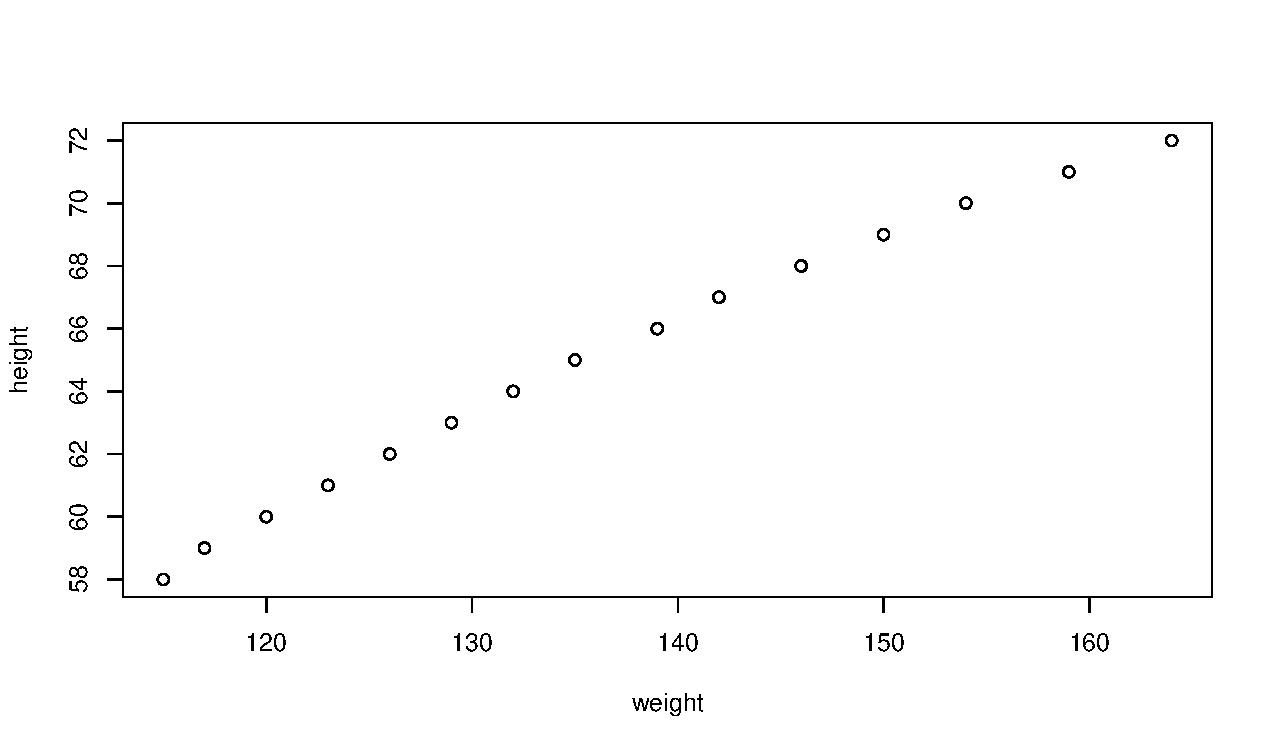
\includegraphics[width=\maxwidth]{figure/unnamed-chunk-33-1} 

}


\end{knitrout}
% \end{noindent}
\subsection*{Example: Wald Confidence Interval for Cyclone Data}
\textcolor{Blue}{Wald} based interval: $ \Set*{\theta\given (\hat{\theta}-\theta)I(\hat{\theta})<\chi^2_{(1)}(1-\alpha)} $.
\begin{itemize}
      \item For the Poisson distribution $ \hat{\theta}=\bar{y} $ and
            \[ I(\hat{\theta})=\frac{1}{\hat{\theta}^2}\sum y_i=\frac{n\bar{y}}{\bar{y}^2} =\frac{n}{\bar{y}} \]
      \item So we solve:
            \begin{align*}
                  \hat{\theta}\pm 1.96\bigl(I(\hat{\theta})\bigr)^{-1/2}
                   & =\bar{y}\pm 1.96(n/\bar{y})^{-1/2} \\
                   & = 5.538462\pm 1.96(0.652714)       \\
                   & = (4.2591, 6.8178)
            \end{align*}
\end{itemize}
The likelihood ratio based \qty{95}{\percent} confidence interval is $(4.36, 6.92)$.

The Wald based \qty{95}{\percent} confidence interval is $(4.26, 6.82)$.
% \begin{noindent}
\begin{knitrout}
\definecolor{shadecolor}{rgb}{0.969, 0.969, 0.969}\color{fgcolor}

{\centering 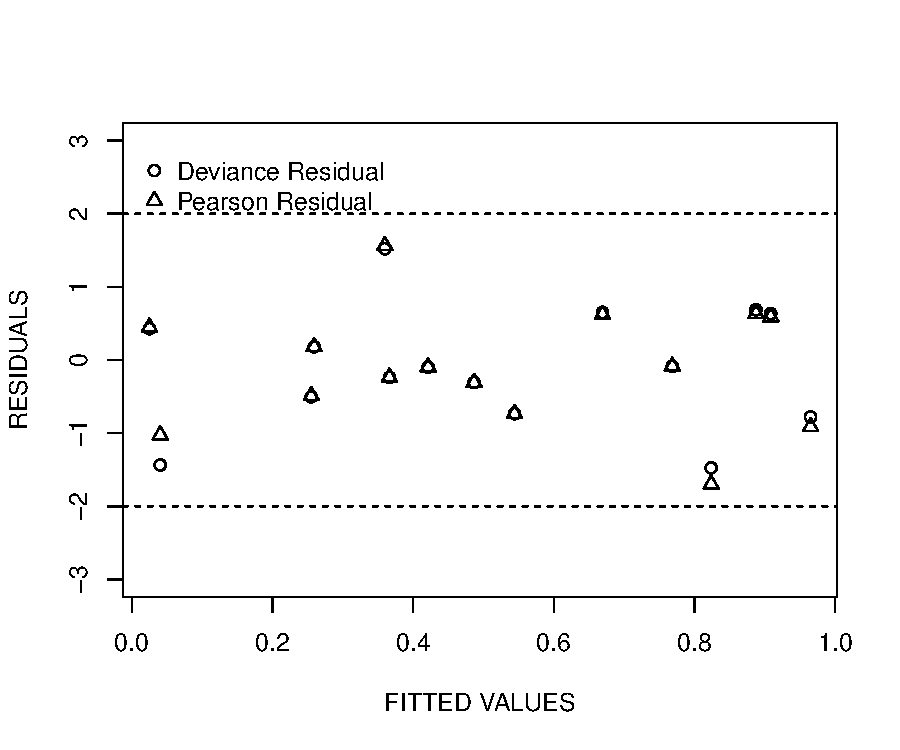
\includegraphics[width=\maxwidth]{figure/unnamed-chunk-34-1} 

}


\end{knitrout}
% \end{noindent}
\subsection*{Testing Hypotheses}
\begin{center}
      $ \HN $: $ \theta=\theta_0 $ vs. $ \HA $: $ \theta\ne \theta_0 $.
\end{center}
\begin{itemize}
      \item \textcolor{Blue}{Likelihood ratio (LR) test}:
            \[ p=\Prob*{\chi^2_{(1)}>-2r(\theta_0)} \]
      \item \textcolor{Blue}{Score test}:
            \[ p=\Prob*{\chi^2_{(1)}>\bigl(S(\theta_0)\bigr)^2/I(\theta_0)} \]
      \item \textcolor{Blue}{Wald test}:
            \[ p=\Prob*{\chi^2_{(1)}>(\hat{\theta}-\theta_0)^2 I(\hat{\theta})} \]
            or
            \[ p=\Prob*{\abs{Z}>\abs*{\theta-\theta_0}\sqrt{I(\hat{\theta})}} \]
\end{itemize}
\subsection*{Example: Hypothesis Tests for Cyclone Data}
Suppose we wish to test whether there were an average of 5 cyclones per year
\begin{center}
      $ \HN $: $ \theta=5 $ vs. $ \HA $: $ \theta\ne 5 $.
\end{center}
\begin{itemize}
      \item \textcolor{Blue}{Likelihood Ratio} based test:
            \[ r(\theta_0=5)=n\bar{y}\log*{\frac{5}{\bar{y}}}-n(5-\bar{y})=-0.3641 \]
            The $ p $-value for this test is:
            \[ p=\Prob*{\chi^2_{(1)}>-2r(5)}=\Prob*{\chi^2_{(1)}>0.7282}=0.3934 \]
            Therefore we \emph{do not reject} $ \HN $.
\end{itemize}
\subsection*{Notes on Asymptotic Inference}
\begin{itemize}
      \item Asymptotic results: approximation improves as sample size increases.
      \item Results are exact for a Normal linear model if $ \theta $ is the mean parameter and $ \sigma^2 $ is
            known.
      \item \textcolor{Blue}{LR approach}:
            \begin{itemize}
                  \item Need to evaluate (log) likelihood at two locations.
                  \item Not always a closed from solution for a CI\@.
                  \item Usually the best approach.
            \end{itemize}
      \item \textcolor{Blue}{Score approach}:
            \begin{itemize}
                  \item Usually the least powerful test.
                  \item Don't actually need to find MLE to use.
            \end{itemize}
      \item \textcolor{Blue}{Wald's approach}:
            \begin{itemize}
                  \item Always get a closed form solution for a CI\@.
                  \item May not behave well for skewed likelihoods (transform?).
            \end{itemize}
      \item All three are asymptotically equivalent!
\end{itemize}
\subsection*{Likelihood Methods for Parameter Vectors (A3)}
\addcontentsline{toc}{subsection}{Likelihood Methods for Vector}
Suppose $ \Vector{\theta}\in \Omega $ is a continuous $ p\times 1 $ parameter vector indexing a probability density
or mass function $ f(\Vector{y}\mid\Vector{\theta}) $.
\begin{itemize}
      \item $ \mathcal{L}( \Vector{\theta}) $ is the \textcolor{Blue}{Likelihood function}.
      \item $ \ell( \Vector{\theta})=\log[\big]{\mathcal{L}(\Vector{\theta})} $ is the \textcolor{Blue}{log-likelihood function}.
      \item $ \Vector{S}(\Vector{\theta})=\pdv{\ell( \Vector{\theta})}{ \Vector{\theta}} $ is the $ p\times 1 $ \textcolor{Blue}{Score vector}.
      \item $ \Matrix{I}(\Vector{\theta})=-\pdv{\ell(\Vector{\theta})}{ \Vector{\theta}^\top,\Vector{\theta}} $ is the $ p\times p $ \textcolor{Blue}{Information matrix}.
      \item $ R(\Vector{\theta})=\mathcal{L}(\Vector{\theta})/\mathcal{L}(\hat{ \Vector{\theta}}) $ is the \textcolor{Blue}{Relative likelihood function}.
      \item $ r(\Vector{\theta})=\log[\big]{\mathcal{L}(\Vector{\theta})/\mathcal{L}(\hat{\Vector{\theta}})}=\ell(\Vector{\theta})-\ell(\hat{\Vector{\theta}}) $ is the
            \textcolor{Blue}{log relative likelihood function}.
\end{itemize}
\begin{itemize}
      \item The Newton Raphson algorithm applies as before, but with vectors and matrices
            as follows:
            \[ \Vector{\theta}_{i+1}=\Vector{\theta}_i+\bigl(\Matrix{I}(\Vector{\theta})\bigr)^{-1}\Vector{S}(\Vector{\theta}) \]
      \item Again, we apply iteratively until we obtain convergence, but now check to
            see if $ \Matrix{I}(\Vector{\theta}) $ is a positive definite matrix.
      \item Analogs to the LR, Score and Wald results apply based on partitioning the
            Information matrix by $ \Vector{\theta}=(\Vector{\alpha},\Vector{\beta})^\top $,
            where $ \Vector{\alpha} $ is a $ p\times 1 $ vector of nuisance parameters and $ \Vector{\beta} $ is a $ q\times 1 $ vector of parameters of interest:
            \[ \Matrix{I}=\Matrix{I}(\Vector{\alpha},\Vector{\beta})=\begin{pmatrix}
                        \Matrix{I}_{\Vector{\alpha}\Vector{\alpha}}(\Vector{\alpha},\Vector{\beta}) & \Matrix{I}_{\Vector{\alpha}\Vector{\beta}}(\Vector{\alpha},\Vector{\beta}) \\
                        \Matrix{I}_{\Vector{\beta}\Vector{\alpha}}(\Vector{\alpha},\Vector{\beta})  & \Matrix{I}_{\Vector{\beta}\Vector{\beta}}(\Vector{\alpha},\Vector{\beta})
                  \end{pmatrix} \]
            where
            $ \Matrix{I}_{\Vector{\alpha}\Vector{\alpha}}(\Vector{\alpha},\Vector{\beta})=-\pdv{\ell}{\Vector{\alpha},\Vector{\alpha}^\top} $ is $ p\times p $,
            $ \Matrix{I}_{\Vector{\alpha}\Vector{\beta}}(\Vector{\alpha},\Vector{\beta})=-\pdv{\ell}{\Vector{\alpha},\Vector{\beta}^\top} $ is $ p\times q $,
            $ \Matrix{I}_{\Vector{\beta}\Vector{\alpha}}(\Vector{\alpha},\Vector{\beta})=-\pdv{\ell}{\Vector{\beta},\Vector{\alpha}^\top} $ is $ q\times p $, and
            $ \Matrix{I}_{\Vector{\beta}\Vector{\beta}}(\Vector{\alpha},\Vector{\beta})=-\pdv{\ell}{\Vector{\beta},\Vector{\beta}^\top} $ is $ q\times q $.
\end{itemize}

\makeheading{Week 3}{\daterange{2021-09-20}{2021-09-24}}
\section*{Topic 1c: Likelihood for Generalized Linear Models}
\addcontentsline{toc}{section}{Topic 1c: Likelihood for Generalized Linear Models}
\subsection*{Likelihood for Generalized Linear Models}
Recall Stat 331/371: Assume $ Y_i \sim \N{\mu_i,\sigma^2} $ independently. For linear regression:
\[ \E{Y_i}=\Vector{x}_i^\top \Vector{\beta} \]
How can we do regression analysis if the distribution of $Y_i$ is not Normal?
\begin{enumerate}[1.]
      \item Definition of the \textcolor{Blue}{Exponential Family}.
            \begin{itemize}
                  \item Derivation of general likelihood results for the Score and Information.
                  \item Application of general results to the Exponential Family.
                  \item Definition of the canonical link.
                  \item Poisson example.
            \end{itemize}
      \item Definition of a \textcolor{Blue}{Generalized Linear Model}.
\end{enumerate}
\subsection*{The Exponential Family}
\addcontentsline{toc}{subsection}{Exponential Family}
\begin{Regular}{Definition (Exponential Family)}
      Consider a random variable $ Y_i $ with p.d.f.\ $ f(y_i\mid \theta_i,\phi) $, $ \theta_i $
      unknown, $ \phi $ known. We say that
      the distribution is a member of the \textcolor{Blue}{exponential family} if we can write the p.d.f.\ in the
      form:
      \[ f(y_i\mid \theta_i,\phi)=\exp[\bigg]{\frac{\bigl(y_i\theta_i-b(\theta_i)\bigr)}{a_i(\phi)}+c(y_i\mid \phi)} \]
      for some specific functions $ a_i(\:\cdot\:) $, $ b(\:\cdot\:) $, and $ c(\:\cdot\:) $.
\end{Regular}
\begin{itemize}
      \item The parameter $ \theta_i $ is called the \textcolor{Blue}{canonical parameter}.
      \item The parameter $ \phi $, termed the \textcolor{Blue}{scale/dispersion parameter}, is constant and assumed
            to be known.
\end{itemize}
\subsection*{Likelihood for the Exponential Family}
Consider a single observation $ y_i $ from the exponential family.
\begin{itemize}
      \item \textcolor{Blue}{Likelihood}:
            \[ \mathcal{L}_i(\theta_i,\phi\mid y_i)=f(y_i\mid \theta_i,\phi)=\exp[\bigg]{\frac{\bigl(y_i\theta_i-b(\theta_i)\bigr)}{a_i(\phi)}+c(y_i\mid \phi)} \]
      \item \textcolor{Blue}{Log-likelihood}:
            \[ \ell_i(\theta_i,\phi\mid y_i)=\log[\big]{f(y_i\mid \theta_i,\phi)}=\frac{\bigl(y_i\theta_i-b(\theta_i)\bigr)}{a_i(\phi)}+c(y_i\mid \phi) \]
      \item \textcolor{Blue}{Score}:
            \[ S_i(\theta_i)=\pdv{\ell_i}{\theta_i}=\frac{y_i-b^\prime(\theta_i)}{a_i(\phi)} \]
      \item \textcolor{Blue}{Observed Information}:
            \[ I_i(\theta_i)=\pdv[order=2]{\ell_i}{\theta_i}=\frac{b^{\prime\prime}(\theta_i)}{a_i(\phi)} \]
      \item \textcolor{Blue}{Fisher/Expected Info}:
            \[ \mathcal{I}_i(\theta_i)=\E*{-\pdv[order=2]{\ell_i}{\theta_i}} \]
\end{itemize}
\subsection*{Aside: General Results for the Score and Information}
\textcolor{Blue}{Fact}: Probability density functions integrate to 1. Using this,
\begin{align*}
      \int f(y_i\mid \theta_i,\phi)\odif{y_i}                  & =1                         \\
      \pdv*{\int f(y_i\mid \theta_i,\phi)\odif{y_i}}{\theta_i} & =\pdv{1}{\theta_i}         \\
      \int \pdv*{f(y_i\mid \theta_i,\phi)}{\theta_i}\odif{y_i} & =0\label{1c:eq1}\tag*{(1)}
\end{align*}
When differentiating the log-likelihood we have:
\begin{align*}
      \pdv*{\log[\big]{f(y_i\mid \theta_i,\phi)}}{\theta_i}                         & =\frac{1}{f(y_i\mid \theta_i,\phi)}\pdv*{f(y_i\mid \theta_i,\phi)}{\theta_i} \\
      f(y_i\mid \theta_i,\phi)\pdv*{\log[\big]{f(y_i\mid \theta_i,\phi)}}{\theta_i} & =\pdv*{f(y_i\mid \theta_i,\phi)}{\theta_i}\label{1c:eq2}\tag*{(2)}
\end{align*}
Substituting~\ref{1c:eq2} into~\ref{1c:eq1} we get:
\begin{align*}
      \int f(y_i\mid \theta_i,\phi)\pdv*{\log[\big]{f(y_i\mid \theta_i,\phi)}}{\theta_i}\odif{y_i} & =0\label{1c:eq3}\tag*{(3)} \\
      \int f(y_i\mid \theta_i,\phi)S_i(\theta_i)\odif{y_i}                                         & =0                         \\
      \textcolor{Red}{\E*{S_i(\theta_i)}}                                                          & =0
\end{align*}
since by definition $ \displaystyle \E*{g(X)}=\int g(x)f(x\mid \theta)\odif{x} $.
\begin{Result}{Result \# 1}
      The expectation of the score function is zero.
      \[ \E*{S_i(\theta_i)}=0 \]
\end{Result}
Differentiate~\ref{1c:eq3} again:
\begin{align*}
      0                 & =\int f(y_i\mid \theta_i,\phi)\pdv*{\log[\big]{f(y_i\mid \theta_i,\phi)}}{\theta_i}\odif{y_i}                                                                                                                                                                                                          \\
      \pdv{0}{\theta_i} & =\pdv*{\int f(y_i\mid \theta_i,\phi)\pdv*{\log[\big]{f(y_i\mid \theta_i,\phi)}}{\theta_i}\odif{y_i}}{\theta_i}                                                                                                                                                                                         \\
      0                 & =\int \biggl[\pdv*[order=2]{\log[\big]{f(y_i\mid \theta_i,\phi)}}{\theta_i}\biggr]f(y_i\mid \theta_i,\phi)\odif{y_i}+\int \pdv*{\log[\big]{f(y_i\mid \theta_i,\phi)}}{\theta_i}\biggl[\textcolor{Blue}{\pdv*{f(y_i\mid \theta_i,\phi)}{\theta_i}}\biggr]\odif{y_i}                                     \\
      0                 & =\int \pdv*[order=2]{\log[\big]{f(y_i\mid \theta_i,\phi)}}{\theta_i}f(y_i\mid \theta_i,\phi)\odif{y_i}+\int \biggl(\pdv*{\log[\big]{f(y_i\mid \theta_i,\phi)}}{\theta_i}\biggr)^{\!2}f(y_i\mid \theta_i,\phi)\odif{y_i}                                                   &  & \text{Sub~\ref{1c:eq2}} \\
      0                 & =\E*{\pdv*[order=2]{\log[\big]{f(y_i\mid \theta_i,\phi)}}{\theta_i}}+\E*{\biggl(\pdv*{\log[\big]{f(y_i\mid \theta_i,\phi)}}{\theta_i}\biggr)^{\!2}}                                                                                              \label{1c:eq4}\tag*{(4)}
\end{align*}
Examining~\ref{1c:eq4} we get:
\begin{align*}
      \E*{\pdv*[order=2]{\log[\big]{f(y_i\mid \theta_i,\phi)}}{\theta_i}}+\E*{\biggl(\pdv*{\log[\big]{f(y_i\mid \theta_i,\phi)}}{\theta_i}\biggr)^{\!2}} & =0                                                           \\
      \E*{-I_i(\theta_i)}+\E*{S_i(\theta_i)^2}                                                                                                           & =0                                                           \\
      \textcolor{Red}{\E*{S_i(\theta_i)^2}}                                                                                                              & =\textcolor{Red}{\E*{I_i(\theta_i)}=\mathcal{I}_i(\theta_i)}
\end{align*}
\begin{Result}{Result \# 2}
      The expectation of the score function squared is the expected information.
      \[  \E*{S_i(\theta_i)^2}=\E*{I_i(\theta_i)}=\mathcal{I}_i(\theta_i) \]
\end{Result}
Recall that $ \Var*{X}=\E*{X^2}-\bigl(\E{X}\bigr)^2 $. Using Results \#1 and \#2 we have:
\begin{align*}
      \Var*{S_i(\theta_i)} & =\E*{S_i(\theta_i)^2}-\E*{S_i(\theta_i)}^2 \\
                           & =\mathcal{I}_i(\theta_i)-0^2               \\
                           & =\mathcal{I}_i(\theta_i)
\end{align*}
\begin{Result}{Result \# 3}
      The variance of the score function is the expected information:
      \[ \Var*{S_i(\theta_i)}=\mathcal{I}_i(\theta_i) \]
\end{Result}
\subsection*{Applying these Results to the Exponential Family}
\begin{align*}
      \E{S_i(\theta_i)}                             & =0                                     \\
      \E*{\frac{Y_i-b^\prime(\theta_i)}{a_i(\phi)}} & =0                                     \\
      \textcolor{Green}{\E{Y_i}}                    & =\textcolor{Green}{b^\prime(\theta_i)} \\
\end{align*}
\begin{align*}
      \E*{S_i(\theta_i)^2}                                              & =\E*{I_i(\theta_i)}                                      \\
      \E*{\biggl(\frac{Y_i-b^\prime(\theta_i)}{a_i(\phi)}\biggr)^{\!2}} & =\E*{\frac{b^{\prime\prime}(\theta_i)}{a_i(\phi)}}       \\
      \frac{1}{a_i(\phi)^2}\E*{(Y_i-\E*{Y_i})^2}                        & = \frac{b^{\prime\prime}(\theta_i)}{a_i(\phi)}           \\
      \textcolor{Green}{\Var{Y_i}}                                      & = \textcolor{Green}{b^{\prime\prime}(\theta_i)a_i(\phi)}
\end{align*}
\subsection*{Properties of the Exponential Family}
For a random variable $Y_i$ with a distribution in the exponential family, $ \theta_i $ unknown, $ \phi $
known:
\[ \mathcal{L}_i(\theta_i,\phi\mid y_i)=f(y_i\mid \theta_i,\phi)=\exp[\bigg]{\frac{\bigl(y_i\theta_i-b(\theta_i)\bigr)}{a_i(\phi)}+c(y_i\mid \phi)} \]
\begin{Regular}{Mean and Variance for the Exponential Family}
      \begin{itemize}
            \item Mean: $ \E{Y_i}=b^\prime(\theta_i)=\mu_i $.
            \item Variance: $ \Var{Y_i}=b^{\prime\prime}(\theta_i)a_i(\phi) $
      \end{itemize}
\end{Regular}
\begin{itemize}
      \item $ \V{\mu_i}=b^{\prime\prime}(\theta_i) $ is called the \textcolor{Blue}{Variance function}.
      \item $ b^{\prime\prime}(\theta_i) $ is a function of the \textcolor{Blue}{canonical parameter} $ \theta_i $ and hence a function of the mean
            (mean-variance relationship)
      \item $ a_i(\phi) $ is a known function of the \textcolor{Blue}{dispersion parameter} $ \phi $.
      \item Often we can write $ a_i(\phi)=\phi/w_i $ where $ w_i $ is a weight.
\end{itemize}
\subsection*{Link Functions}
\begin{Regular}{Definition (Link Function)}
      The \textcolor{Blue}{link function} $ g(\mu_i) $ relates the \textcolor{Blue}{linear predictor} $ \eta_i=\Vector{x}^\top\Vector{\beta} $ to the expected value $ \mu_i $ of the random variable $ Y_i $.
      \[ g(\mu_i)=\eta_i=\Vector{x}_i^\top\Vector{\beta} \]
\end{Regular}
\begin{Regular}{Definition (Canonical Link Function)}
      When $Y_i$ is a member of the \textcolor{Blue}{exponential family} we define the \textcolor{Blue}{canonical link function} to be:
      \[ g(\mu_i)=\theta_i=\eta_i=\Vector{x}_i^\top\Vector{\beta} \]
      (i.e., canonical parameter = linear predictor)
\end{Regular}
\subsection*{Examples}
Many well known distributions belong to the exponential family:
\begin{itemize}
      \item \textcolor{Blue}{Normal distribution}: $ Y \sim \N{\mu,\sigma^2} $, $ \sigma^2 $ known.
            \[ f(y\mid \theta,\phi)=\frac{1}{\sqrt{2\pi\sigma^2}} \exp*{-\frac{(y-\mu)^2}{2\sigma^2}},\qquad y\in(-\infty,\infty) \]
      \item \textcolor{Blue}{Poisson Distribution}: $ Y \sim \POI{\lambda} $.
            \[ f(y\mid \lambda)=\frac{\lambda^y e^{-\lambda}}{y!},\qquad y=0,1,2,\ldots  \]
      \item \textcolor{Blue}{Binomial Distribution}: $ Y \sim \BIN{m,\pi} $.
            \[ f(y\mid \pi)=\binom{m}{y}\pi^y(1-\pi)^{m-y},\qquad y=0,1,\ldots,m \]
\end{itemize}
\begin{Example}{The Poisson Distribution}
      Let $ Y_i $, $ i=1,2,\ldots,n $ be iid $ \POI{\lambda_i} $.
      \[ f(y_i\mid \lambda_i)=\frac{\lambda_i^{y_i} e^{-\lambda_i}}{y_i!},\qquad y_i=0,1,2,\ldots \]
      Show that the distribution of $ Y_i $ is a member of the exponential family and find the
      mean, variance, variance function and canonical link function.
\end{Example}
\subsection*{Exponential Family: Full Disclosure}
The definition of the exponential family used in the Stat 431 course notes is actually a
special case of:
\begin{Regular}{Definition (General Exponential Family)}
      A distribution is a member of the \textcolor{Blue}{General Exponential Family} if it can be expressed as:
      \[ f(y\mid \Vector{\theta})=\exp[\bigg]{\sum_{i=1}^{k} w_i(\Vector{\theta})t_i(y)+b(\Vector{\theta})+h(y)} \]
      for $ t_1(y),\ldots,t_k(y) $ real-valued function of $ y $, and $ w_1(\Vector{\theta}),\ldots,w_k(\Vector{\theta}) $ real-valued
      functions of the possibly vector-valued parameter $ \Vector{\theta} $.
\end{Regular}
\subsection*{Random Sample from the Exponential Family}
Now suppose $ Y_i $, $ i=1,2,\ldots,n $ are iid with a distribution that is a member of the
\textcolor{Blue}{exponential family}. Then:
\[ \mathcal{L}(\Vector{\theta},\phi\mid \Vector{y})=\prod_{i=1}^n f(y_i\mid \theta_i,\phi)=\prod_{i=1}^n\exp[\bigg]{\frac{\bigl(y_i\theta_i-b(\theta_i)\bigr)}{a_i(\phi)}+c(y_i\mid \phi)} \]
\[ \ell(\Vector{\theta},\phi\mid \Vector{y})=\sum_{i=1}^n \log[\big]{f(y_i\mid \theta_i,\phi)}=\sum_{i=1}^n \biggl(\frac{\bigl(y_i\theta_i-b(\theta_i)\bigr)}{a_i(\phi)}+c(y_i\mid \phi)\biggr) \]
In a regression context, we are interested in estimating $ \Vector{\beta} $ under the \textcolor{Blue}{link function}:
\[ g(\mu_i)=\Vector{x}_i^\top\Vector{\beta} \]
where $ \Vector{x}_i $ is a vector of explanatory variables for subject $ i=1,2,\ldots, n $.
\subsection*{Generalized Linear Models}
\addcontentsline{toc}{subsection}{Generalized Linear Models}
\begin{Regular}{Definition (Generalized Linear Model (GLM))}
      A \textcolor{Blue}{Generalized Linear Model (GLM)} is composed of:
      \begin{itemize}
            \item The \textcolor{Blue}{Random Component}: The distribution of the iid response variables $ Y_i $ is
                  assumed to come from a parametric distribution that is a member of the
                  exponential family.
            \item The \textcolor{Blue}{Systematic Component} or linear predictor $ \eta_i=\Vector{x}_i^\top\Vector{\beta} $, a linear combination of
                  explanatory variables $ \Vector{x}_i $ and regression parameters $ \Vector{\beta} $.
            \item The \textcolor{Blue}{Link function} that relates the mean of the distribution of $ Y_i $ to the linear
                  predictor through:
                  \[ g(\mu_i)=\eta_i=\Vector{x}_i^\top\Vector{\beta} \]
      \end{itemize}
\end{Regular}
\subsection*{Topic Summary: Likelihood for Generalized Linear Models}
\begin{enumerate}[1.]
      \item Definition of the \textcolor{Blue}{Exponential Family}.
            \begin{itemize}
                  \item Derivation of general likelihood results for the Score and Information.
                  \item Application of general results to the Exponential Family.
                  \item Definition of the canonical link.
                  \item Poisson example.
            \end{itemize}
      \item Definition of a \textcolor{Blue}{Generalized Linear Model}.
\end{enumerate}
\textcolor{Blue}{Next Topic: Estimation for Generalized Linear Models}.
\begin{itemize}[label={}]
      \item Estimation of $ \Vector{\beta} $ from a GLM through Iteratively Reweighted Least Squares
            (IRWLS).
\end{itemize}

\section*{Topic 1d: Estimation for GLMs}
\addcontentsline{toc}{section}{Topic 1d: Estimation for GLMs}
\subsection*{Generalized Linear Models}
\addcontentsline{toc}{subsection}{GLM Definition}
\begin{Regular}{Definition}
    A \textcolor{Blue}{Generalized Linear Model (GLM)} is composed of:
    \begin{enumerate}[1.]
        \item The \textcolor{Blue}{Random Component}: The distribution of the response variables $ Y_i $ is
              assumed to come from a parametric distribution that is a member of the
              exponential family \textcolor{Blue}{Systematic Component} or linear predictor $ \eta_i =\Vector{x}_i^\top\Vector{\beta} $, a linear
              combination of explanatory variables $ \Vector{x}_i $ and regression parameters $ \Vector{\beta} $
              that relates the mean of the distribution of $ Y_i $ to the linear predictor through
              \[ g(\mu_i)=\eta_i=\Vector{x}_i^\top\Vector{\beta} \]
    \end{enumerate}
\end{Regular}
\subsection*{Estimation of $ \Vector{\beta} $ from a GLM through IRWLS}
\addcontentsline{toc}{subsection}{Iteratively Reweighted Least Squares}
Consider the log-likelihood for a single observation from the exponential family:
\[ \ell_i(\theta_i,\phi\mid y_i)=\frac{y_i\theta_i-b(\theta_i)}{a_i(\phi)}+c(y_i;\phi) \]
\begin{itemize}
    \item $ \ell_i $ is a function of $ \theta_i $ (assume that $ \phi $ is known).
    \item $ \mu_i $ can be expressed in terms of $ \theta_i $ through the mean:
          \[ \mu_i=b^\prime(\theta_i) \]
    \item $ \eta_i $ can be expressed in terms of $ \mu_i $ through the link function:
          \[ \eta_i=g(\mu_i) \]
    \item $ \Vector{\beta} $ can be expressed in terms of $ \Vector{\eta} $ through the linear predictor:
          \[ \Vector{x}_i^\top \Vector{\beta}=\eta_i \]
\end{itemize}
Thus, $ \ell_i(\theta_i,\phi\mid y_i) $ depends on $ \theta_i $, so $ \theta_i $ depends on $ \mu_i $, so $ \mu_i $ depends on $ \eta_i $, and so $ \eta_i $ depends on $ \beta_j $.
Therefore, we will use the chain rule on:
\[ \ell_i(\beta_j)=f\biggr(\theta_i\Bigl(\mu_i\bigl(\eta_i(\beta_j)\bigr)\Bigr)\biggr) \]
\subsection*{The Score Vector}
\addcontentsline{toc}{subsubsection}{The Score Vector}
Using \textcolor{Blue}{Maximum Likelihood} to estimate $ \Vector{\beta} $, we must solve $ \Vector{S}(\Vector{\beta})=\Vector{0}_p $.
Consider the $ j^{\text{th}} $ element of the score vector:
\[ \pdv{\ell_i}{\beta_j}=\pdv{\ell_i}{\theta_i}\pdv{\theta_i}{\mu_i}\pdv{\mu_i}{\eta_i}\pdv{\eta_i}{\beta_j} \]
where
\begin{align*}
    \pdv{\ell_i}{\theta_i} & =\frac{y_i-b^\prime(\theta_i)}{a_i(\phi)}=\frac{y_i-\mu_i}{a_i(\phi)}                                            &  & \text{since $b^\prime(\theta_i)=\mu_i$}                                                                  \\
    \pdv{\theta_i}{\mu_i}  & =\biggl(\pdv{\mu_i}{\theta_i}\biggr)^{\!-1}  =\frac{1}{b^{\prime\prime}(\theta_i)}=\frac{a_i(\phi)}{\Var{\mu_i}} &  & \text{since $\mu_i=b^{\prime}(\theta_i)$, $\Var{\mu_i}=b^{\prime\prime}(\theta_i)a_i(\phi)$}             \\
    \pdv{\mu_i}{\eta_i}    & =\pdv{\mu_i}{\eta_i}                                                                                             &  & \text{(depends on selected link)}                                                                        \\
    \pdv{\eta_i}{\beta_j}  & =x_{ij}                                                                                                          &  & \text{since $\Vector{x}_i^\top \Vector{\beta}=\eta_i=\sum_{j=0}^{p-1}x_{ij}\beta_j$, for $i=1,\ldots,n$}
\end{align*}
So we have
\begin{align*}
    \pdv{\ell_i}{\beta_j}
     & =\frac{y_i-\mu_i}{a_i(\phi)}\frac{a_i(\phi)}{\Var{\mu_i}}\pdv{\mu_i}{\eta_i}x_{ij}                                                                              \\
     & =\frac{y_i-\mu_i}{\Var{y_i}}\biggl(\pdv{\mu_i}{\eta_i}\biggr)^{\!2}\pdv{\eta_i}{\mu_i}x_{ij} &  & \text{multiply by $1=\pdv{\mu_i}{\eta_i}\pdv{\eta_i}{\mu_i}$} \\
     & =(y_i-\mu_i)w_i\pdv{\eta_i}{\mu_i}x_{ij}
\end{align*}
where $ w_i=\frac{1}{\Var{Y_i}(\pdv{\eta_i}{\mu_i})^2} $. Note that generally $ \pdv{\eta_i}{\mu_i} $ is easier to calculate than $ \pdv{\mu_i}{\eta_i} $
since we define the link as $ \eta_i=g(\mu_i) $.

With $ n $ iid observations, the $ j^{\text{th}} $ element of the score vector is:
\begin{Regular}{}
    \[ \bigl[ \Vector{S}(\Vector{\beta})\bigr]_j=\sum_{i=1}^{n} \pdv{\ell_i}{\beta_j}=\sum_{i=1}^{n} (y_i-\mu_i)w_i\pdv{\eta_i}{\mu_i}x_{ij}\quad\text{for $j=0,1,\ldots,p-1$} \]
\end{Regular}
In vector form we can write:
\begin{Regular}{}
    \[ \Vector{S}(\Vector{\beta})=\Matrix{X}\Matrix{W}(\Vector{y}-\Vector{\mu})\circ \pdv{\Vector{\eta}}{\Vector{\mu}} \]
\end{Regular}
where $ \Vector{y}=(y_1,\ldots,y_n)^\top $ and $ \Vector{\mu}=(\mu_1,\ldots,\mu_n)^\top $ are $ n\times 1 $ vectors, $ \Matrix{X}=(\Vector{x}_1,\ldots,\Vector{x}_n) $
is a $ p\times n $ matrix, $ \Matrix{W} $ denotes the $ n\times n $ diagonal matrix with $ \Matrix{W}=\diag{w_1,w_2,\ldots,w_n} $,
$ \circ $ denotes an element-wise product, and $ \pdv{\Vector{\eta}}{\Vector{\mu}}=\bigl(\pdv{\eta_1}{\mu_1},\pdv{\eta_2}{\mu_2},\ldots,\pdv{\eta_n}{\mu_n}\bigr)^\top $.
\subsection*{}
\addcontentsline{toc}{subsection}{Poisson Example}
\begin{Example}{Example: The Poisson Distribution (Problem 1.4)}
    Let $ Y_i $, $ i=1,\ldots,n $ be independent Poisson random variables with $ \E{Y_i}=\lambda_i $. Suppose
    that associated with each $ y_i $ is a $ p\times 1 $ vector of explanatory variables $ \Vector{x}_i $. A Poisson
    regression model with the canonical link takes the form:
    \[ \log{\lambda_i}=\beta_0+\beta_1x_{i1}+\cdots+\beta_{p-1}x_{i(p-1)}=\Vector{x}_i^\top \Vector{\beta} \]
    To answer the following you may either calculate the derivatives using standard
    methods, or use the general results derived in class for the exponential family.
    \begin{enumerate}[a.]
        \item Write down the score vector for the regression coefficients $ \Vector{\beta} $.
    \end{enumerate}
\end{Example}
\subsection*{Newton Raphson and Fisher Scoring}
To solve $ \Vector{S}(\Vector{\beta})=\Vector{0}_p $, the \textcolor{Blue}{Newton Raphson} update equation is:
\[ \hat{\Vector{\beta}}^{(r+1)}=\hat{\Vector{\beta}}^{(r)}+\Matrix{I}^{-1}\bigl(\hat{\Vector{\beta}}^{(r)}\bigr)\Vector{S}\bigl(\hat{\Vector{\beta}}^{(r)}\bigr) \]
where $ \Matrix{I}(\:\cdot\:) $ is the observed information matrix.
\begin{itemize}
    \item This requires us to find and repeatedly evaluate the Information $ \Matrix{I}(\:\cdot\:) $ (possibly computational intensive).
    \item Fisher suggested using the expected information matrix $ \mathcal{I}(\:\cdot\:) $ rather than the observed information matrix.
\end{itemize}
The \textcolor{Blue}{Fisher Scoring} update equation is:
\[ \hat{\Vector{\beta}}^{(r+1)}=\hat{\Vector{\beta}}^{(r)}+\mathcal{I}^{-1}\bigl(\hat{\Vector{\beta}}^{(r)}\bigr)\Vector{S}\bigl(\hat{\Vector{\beta}}^{(r)}\bigr) \]
\subsection*{The Information Matrix}
Consider the $(j, k)$ element of the Information matrix:
\begin{align*}
    I_{jk} & =-\pdv{\ell_i}{\beta_j,\beta_k}                                                                                                                                                           \\
           & =-\pdv*{\pdv{\ell_i}{\beta_j}}{\beta_k}                                                                                                                                                   \\
           & =-\pdv*{\biggl[(y_i-\mu_i)w_i\biggl(\pdv{\eta_i}{\mu_i}\biggr)x_{ij}\biggr]}{\beta_k}                                                                                                     \\
           & =-(y_i-\mu_i)\Biggl\{\pdv*{\biggl[w_i\biggl(\pdv{\eta_i}{\mu_i}\biggr)x_{ij}\biggr]}{\beta_k}\Biggr\}-w_i\biggl(\pdv{\eta_i}{\mu_i}\biggr)x_{ij}\biggl[\pdv*{(y_i-\mu_i)}{\beta_k}\biggr] \\
           & =-(y_i-\mu_i)\Biggl\{\pdv*{\biggl[w_i\biggl(\pdv{\eta_i}{\mu_i}\biggr)x_{ij}\biggr]}{\beta_k}\Biggr\}+w_i\biggl(\pdv{\eta_i}{\mu_i}\biggr)x_{ij}\pdv{\mu_i}{\eta_i}x_{ik}                 \\
           & =-(y_i-\mu_i)\pdv*{\biggl[w_i\biggl(\pdv{\eta_i}{\mu_i}\biggr)x_{ij}\biggr]}{\beta_k}+x_{ij}w_i x_{ik}
\end{align*}
Where the above holds since
\[ g(\mu_i)=\eta_i=\Vector{x}_i^\top \Vector{\beta}\implies \pdv{\mu_i}{\beta_k}=\pdv{\mu_i}{\eta_i}\pdv{\eta_i}{\beta_k}=\pdv{\mu_i}{\eta_i}x_{ik} \]
\subsection*{Fisher Scoring}
To get an element of the Expected/Fisher Information matrix:
\begin{align*}
    \mathcal{I}_{jk}
     & =\E*{-\pdv{\ell_i}{\beta_j,\beta_k}}                                                                                                               \\
     & =\E*{-(y_i-\mu_i)\pdv*{\biggl[w_i\biggl(\pdv{\eta_i}{\mu_i}\biggr)x_{ij}\biggr]}{\beta_k}+x_{ij}w_i x_{ik}}                                        \\
     & =\pdv*{\biggl[w_i\biggl(\pdv{\eta_i}{\mu_i}\biggr)x_{ij}\biggr]}{\beta_k}\E*{(y_i-\mu_i)}+x_{ij}w_i x_{ik}                                         \\
     & =x_{ij}w_i x_{ik}                                                                                           &  & \text{since $\E*{(y_i-\mu_i)}=0$}
\end{align*}
Therefore, for $ n $ observations we can write:
\begin{Regular}{}
    \[ \mathcal{I}_{jk}=\sum_{i=1}^{n}x_{ij}w_i x_{ik}=\bigl(\Matrix{X}\Matrix{W}\Matrix{X}^\top\bigr)_{jk} \]
\end{Regular}
where again, $ \Matrix{W}=\diag{w_1,w_2,\ldots,w_n} $ and $ w_i=\frac{1}{\Var{Y_i}(\pdv{\eta_i}{\mu_i})^2} $.
\subsection*{When is Fisher Scoring Equivalent to Newton Raphson?}
Fisher Scoring is equivalent to Newton Raphson when the expected information matrix is equal to the observed information matrix. Recall:
\[ I_{jk}=-(y_i-\mu_i)\pdv*{\biggl[w_i\biggl(\pdv{\eta_i}{\mu_i}\biggr)x_{ij}\biggr]}{\beta_k}+x_{ij}w_i x_{ik} \]
Now examine:
\begin{align*}
    w_i
     & =\frac{1}{\Var{Y_i}} \biggl(\pdv{\mu_i}{\eta_i}\biggr)^{\!2}                                                                                                                                                             \\
     & =\frac{1}{a_i(\phi)b^{\prime\prime}(\theta_i)} \biggl(\pdv{\mu_i}{\eta_i}\biggr) \biggl(\pdv{\mu_i}{\eta_i}\biggr) &  & \text{since $\Var{Y_i}=b^{\prime\prime}(\theta_i)a_i(\phi)$}                                     \\
     & =\frac{1}{a_i(\phi)}\pdv{\theta_i}{\mu_i} \biggl(\pdv{\mu_i}{\eta_i}\biggr) \biggl(\pdv{\mu_i}{\eta_i}\biggr)      &  & \text{and $b^{\prime\prime}(\theta_i)=\pdv{b^\prime(\theta_i)}{\theta_i}=\pdv{\mu_i}{\theta_i}$} \\
     & =\frac{1}{a_i(\phi)} \pdv{\mu_i}{\eta_i}                                                                           &  & \text{under the canonical link $\theta_i=\eta_i$}
\end{align*}
So under the canonical link:
\begin{align*}
    \pdv*{\biggl[w_i\biggl(\pdv{\eta_i}{\mu_i}\biggr)x_{ij}\biggr]}{\beta_k}
     & =\pdv*{\biggl[\frac{1}{a_i(\phi)} \pdv{\mu_i}{\eta_i}\biggl(\pdv{\eta_i}{\mu_i}\biggr)x_{ij}\biggr]}{\beta_k} \\
     & =\pdv*{\biggl(\frac{x_{ij}}{a_i(\phi)}\biggr)}{\beta_k}                                                       \\
     & =0
\end{align*}
We then have:
\[ I_{jk}=-(y_i-\mu_i)\underbracket{\pdv*{\biggl[w_i\biggl(\pdv{\eta_i}{\mu_i}\biggr)x_{ij}\biggr]}{\beta_k}}_{=0}+x_{ij}w_i x_{ik}=x_{ij}w_ix_{ik}=\mathcal{I}_{jk} \]
Therefore under the canonical link, the expected information matrix equals the
observed information matrix and Fisher Scoring is equivalent to Newton Raphson.
\subsection*{Iteratively Reweighted Least Squares (IRWLS)}
Why is this called the iteratively reweighted least squares?
The Fisher Scoring update equation:
\[ \hat{\Vector{\beta}}^{(r+1)}=\hat{\Vector{\beta}}^{(r)}+\mathcal{I}^{-1}\bigl(\hat{\Vector{\beta}}^{(r)}\bigr)\Vector{S}\bigl(\hat{\Vector{\beta}}^{(r)}\bigr) \]
can actually be rewritten as:
\[ \hat{\Vector{\beta}}^{(r+1)}=\Bigl[\Matrix{X}\Matrix{W}\bigl(\hat{\Vector{\beta}}^{(r)}\bigr)\Matrix{X}^\top\Bigr]^{-1}\Matrix{X}\Matrix{W}\bigl(\hat{\Vector{\beta}}^{(r)}\bigr)\Vector{z}\bigl(\hat{\Vector{\beta}}^{(r)}\bigr) \]
\begin{itemize}
    \item See manipulation in Section 1.2.3 of course notes with: $ \Vector{z}=\Vector{\eta}+(\Vector{y}-\Vector{\mu})\circ\pdv{\Vector{\eta}}{\Vector{\mu}} $.
    \item Same form as weighted LS estimate of $ \Vector{\beta} $ with dependent variable $ \Vector{z}\bigl(\hat{\Vector{\beta}}^{(r)}\bigr) $ and weight matrix
          $\Matrix{W}\bigl(\hat{\Vector{\beta}}^{(r)}\bigr) $.
\end{itemize}
\subsection*{Summary}
\begin{itemize}
    \item When $ Y_i $ come from a distribution in the exponential family we can use the theory
          of Generalized Linear Models to fit the regression equations of the form:
          \[ g(\mu_i)=\Vector{x}_i^\top \Vector{\beta} \]
    \item The link function $ g(\:\cdot\:) $ may be the canonical link, but its choice should come from
          model interpretation and fit.
    \item Can use IRWLS to estimate the regression parameters $ \Vector{\beta} $ from any GLM based on
          general forms for $ \Matrix{I}(\Vector{\beta}) $ and $ \Vector{S}(\Vector{\beta}) $.
    \item Practice: Assignment 1 \& Chapter 1 review problems.
\end{itemize}
\begin{Example}{Example: The Poisson Distribution (Problem 1.4)}
    Let $ Y_i $, $ i=1,\ldots,n $ be independent Poisson random variables with $ \E{Y_i}=\lambda_i $. Suppose
    that associated with each $ y_i $ is a $ p\times 1 $ vector of explanatory variables $ \Vector{x}_i $. A Poisson
    regression model with the canonical link takes the form:
    \[ \log{\lambda_i}=\beta_0+\beta_1x_{i1}+\cdots+\beta_{p-1}x_{i(p-1)}=\Vector{x}_i^\top \Vector{\beta} \]
    To answer the following you may either calculate the derivatives using standard
    methods, or use the general results derived in class for the exponential family.
    \begin{enumerate}[a.]
        \item Write down the score vector for the regression coefficients $ \Vector{\beta} $.
        \item Write down the observed and expected information matrix for $ \Vector{\beta} $. Are they the same or different? Why?
        \item What is the form of the weight function? What types of observations will have
              the largest and smallest weights?
    \end{enumerate}
\end{Example}

\section*{Topic 2a: Binary Data: Estimation of the Odds Ratio}
\addcontentsline{toc}{section}{Topic 2a: Binary Data: Estimation of the Odds Ratio}
\begin{enumerate}[1.]
    \item Definition of the Odds Ratio as a measure of association.
    \item Likelihood based estimation of the Odds Ratio.
    \item Inference for the Odds Ratio (Wald based confidence interval).
    \item Example: Prenatal Care.
\end{enumerate}
\subsection*{2.1 Introduction to the Analysis of Binary Data}
\addcontentsline{toc}{subsection}{Odds Ratios}
\begin{itemize}
    \item \textcolor{Blue}{Outcome/Response}: Binary (yes/no, diseased/healthy).
    \item \textcolor{Blue}{Explanatory Variable}: Binary (yes/no, treatment/control).
    \item Use a $ 2\times 2 $ table to summarize the data:
          \begin{table}[!htbp]
              \centering
              \begin{NiceTabular}{l|cc|c}
                  & \multicolumn{2}{c}{\emph{Disease}}                                                 \\
                  & Present                            & Absent                                        \\
                  \midrule
                  Treatment & $ y_1 $                            & $ m_1-y_1 $                 & $ m_1 $         \\
                  Control   & $ y_2 $                            & $ m_2-y_2 $                 & $ m_2 $         \\
                  \midrule
                  & $ y_{\bullet} $                    & $ m_{\bullet}-y_{\bullet} $ & $ m_{\bullet} $
              \end{NiceTabular}
          \end{table}
    \item Treat $ m_1 $ and $ m_2 $ as fixed.
    \item Assume $ Y_k $ are independent binomial random variables:
          \[ \textcolor{Blue}{Y_k \sim \BIN{m_k,\pi_k}\qquad\text{where $0<\pi_k<1$ for $k=1,2$}} \]
    \item $ \pi_k=\Prob*{\text{response}\given \text{group $k$}} $.
\end{itemize}
\subsection*{Definition: Odds}
How do we measure the association between treatment and response?
\begin{Regular}{Definition}
    The \textcolor{Blue}{Odds} is the ratio of the probability
    that an event occurs ($ \pi $) to the
    probability that it does not occur:
    \[ \text{Odds}=\frac{\pi}{1-\pi} \]
\end{Regular}
The odds is a one-to-one monotonically increasing function of $ \pi $ which takes on values on the
non-negative real line.
\subsection*{Measures of Association}
\begin{Regular}{Definition}
    The \textcolor{Blue}{Odds Ratio} is the ratio of the odds of an event occurring in one group to the odds
    of the event occurring in another group:
    \[ \text{Odds Ratio}=\psi=\frac{\pi_1/(1-\pi_2)}{\pi_2/(1-\pi_2)} \]
\end{Regular}
\begin{Regular}{Definition}
    The \textcolor{Blue}{Relative Risk} is the ratio of the probability of an event occurring in one group
    versus another group:
    \[ \text{Relative Risk}=\frac{\pi_1}{\pi_2} \]
\end{Regular}
\begin{itemize}
    \item In the case of a rare disease (i.e., when $ \pi_1 $ and $ \pi_2 $ are very small), then:
          \[ \text{OR}\approx \text{RR} \]
    \item This can be seen by noting that:
          \[ \text{OR}=\psi=\frac{\pi_1/(1-\pi_2)}{\pi_2/(1-\pi_2)}=\frac{\pi_1}{\pi_2} \underbracket{\biggl(\frac{1-\pi_2}{1-\pi_1}\biggr)}_{\approx 1}\approx \frac{\pi_1}{\pi_2} \approx \text{RR}  \]
    \item \textcolor{Blue}{Interpretation of OR}:
          \[ \begin{array}{lcl}
                  \pi_1=\pi_2  \implies & \text{OR}=1   & \implies  \text{equal risk}             \\
                  \pi_1>\pi_2  \implies & \text{OR}>1   & \implies  \text{higher risk in group 1} \\
                  \pi_1<\pi_2  \implies & 0<\text{OR}<1 & \implies  \text{higher risk in group 2}
              \end{array} \]
\end{itemize}
\subsection*{Odds Ratio Example Calculations}
\begin{Example}{}
    \begin{itemize}
        \item $ \pi_1=0.50 $, $ \pi_2=0.25 $, so $ \text{RR}=0.50/0.25=2 $ and $ \text{OR}=\bigl(0.50/0.50\bigr)/\bigl(0.25/0.75\bigr)=3 $.
        \item $ \pi_1=0.10 $, $ \pi_2=0.05 $, so $ \text{RR}=0.10/0.05=2 $ and $ \text{OR}=\bigl(0.10/0.90\bigr)/\bigl(0.05/0.95\bigr)=2.11 $.
        \item  $ \pi_1=0.25 $, $ \pi_2=0.10 $, so $ \text{RR}=0.25/0.10=2.5 $ and $ \text{OR}=\bigl(0.25/0.75\bigr)/\bigl(0.10/0.90\bigr)=3 $.
    \end{itemize}
\end{Example}
\subsection*{2.2 (Likelihood Based) Estimation of the Odds Ratio}
\addcontentsline{toc}{subsection}{Estimation of the Odds Ratio}
\begin{itemize}
    \item \textcolor{Blue}{Goal}: Use Likelihood Theory to estimate $ \text{OR}=\psi=\frac{\pi_1/(1-\pi_1)}{\pi_2/(1-\pi_2)} $.
    \item Assumption: \textcolor{Blue}{$ Y_k \sim \BIN{m_k,\pi_k} $, $ k=1,2 $} independently.
\end{itemize}
\begin{align*}
    \mathcal{L}(\pi_1,\pi_2)
     & =\Prob*{Y_1=y_1,Y_2=y_2\given \pi_1,\pi_2}                                                                                                                                                                  \\
     & =\Prob*{Y_1=y_1\given \pi_1}\Prob*{Y_2=y_2\given \pi_2}                                                                                                                                                     \\
     & =\binom{m_1}{y_1}\pi_1^{y_1}(1-\pi_1)^{m_1-y_1}\binom{m_2}{y_2}\pi_2^{y_2}(1-\pi_2)^{m_2-y_2}                                                                                                               \\
     & \propto \biggl(\frac{\pi_1}{1-\pi_1}\biggr)^{\!y_1}(1-\pi_1)^{m_1}\biggl(\frac{\pi_2}{1-\pi_2}\biggr)^{\!y_2}(1-\pi_2)^{m_2}\textcolor{Blue}{\biggl(\frac{\pi_2/(1-\pi_2)}{\pi_2/(1-\pi_2)}\biggr)^{\!y_1}} \\
     & \propto \biggl(\frac{\pi_1/(1-\pi_1)}{\pi_2/(1-\pi_2)}\biggr)^{\!y_1}\biggl(\frac{\pi_2}{1-\pi_2} \biggr)^{\!y_2+y_1}(1-\pi_1)^{m_1}(1-\pi_2)^{m_2}
\end{align*}
\subsection*{Estimation of the Odds Ratio}
\begin{itemize}
    \item Since we want to estimate $ \psi $, we can \textcolor{Blue}{reparameterize} using:
          \[ \theta_1=\log*{\frac{\pi_1/(1-\pi_1)}{\pi_2/(1-\pi_2)}}=\log{\psi},\qquad \theta_2=\log*{\frac{\pi_2}{1-\pi_2}}  \]
    \item Note that $ \pi_1,\pi_2\in(0,1) $ but $ \theta_1,\theta_2\in(-\infty,\infty) $.
    \item Our reparameterization implies:
          \[ \pi_2=\frac{e^{\theta_2}}{1+e^{\theta_2}},\qquad \pi_1=\frac{e^{\theta_1+\theta_2}}{1+e^{\theta_1+\theta_2}} \]
    \item Now the likelihood becomes:
          \begin{align*}
              \mathcal{L}(\pi_1,\pi_2)       & \propto \biggl(\frac{\pi_1/(1-\pi_1)}{\pi_2/(1-\pi_2)}\biggr)^{\!y_1}\biggl(\frac{\pi_2}{1-\pi_2} \biggr)^{\!y_2+y_1}(1-\pi_1)^{m_1}(1-\pi_2)^{m_2} \\
              \mathcal{L}(\theta_1,\theta_2) & =(e^{\theta_1})^{y_1}(e^{\theta_2})^{y_1+y_2}(1+e^{\theta_1+\theta_2})^{-m_1}(1+e^{\theta_2})^{-m_2}
          \end{align*}
    \item Recall our goal was to estimate $ \text{OR}=\psi=e^{\theta_1} $.
          \begin{align*}
              \mathcal{L}(\theta_1,\theta_2) & =(e^{\theta_1})^{y_1}(e^{\theta_2})^{y_1+y_2}(1+e^{\theta_1+\theta_2})^{-m_1}(1+e^{\theta_2})^{-m_2}                                 \\
              \ell(\theta_1,\theta_2)        & =y_1\theta_1+(y_1+y_2)\theta_2-m_1\log{1+e^{\theta_1+\theta_2}}-m_2\log{1+e^{\theta_2}}                                              \\
              S_1(\theta_1,\theta_2)         & =y_1-m_1\biggl(\frac{e^{\theta_1+\theta_2}}{1+e^{\theta_1+\theta_2}}\biggr)                                                          \\
              S_2(\theta_1,\theta_2)         & =y_1+y_2-m_1\biggl(\frac{e^{\theta_1+\theta_2}}{1+e^{\theta_1+\theta_2}}\biggr)-m_2\biggl(\frac{e^{\theta_2}}{1+e^{\theta_2}}\biggr)
          \end{align*}
    \item Solving $ \Vector{S}(\theta_1,\theta_2)=\Vector{0} $ gives us the MLEs:
          \[ \hat{\theta}_1=\log*{\frac{y_1/(m_1-y_1)}{y_2/(m_2-y_2)}},\qquad \hat{\theta}_2=\log*{\frac{y_2}{m_2-y_2}} \]
    \item So by the invariance property of MLEs we have:
          \[ \hat{\psi}=\frac{\hat{\pi}_1/(1-\hat{\pi}_1)}{\hat{\pi}_2/(1-\hat{\pi}_2)},\qquad\hat{\pi}=\frac{y_1}{m_1},\qquad\hat{\pi}=\frac{y_2}{m_2}  \]
\end{itemize}
\begin{Example}{Example: Prenatal Care Data from Two Clinics}
    Consider the data below describing the relationship between the level of prenatal care
    and fetal mortality.
    \begin{center}
        \begin{NiceTabular}{l|cc|c}
            Level of Care & Died                            & Survived & Total                                        \\
            \midrule
            Intensive & $ 20 $                            & $ 316 $                 & $ 336 $         \\
            Regular   & $ 46 $                            & $ 373 $                 & $ 419 $         \\
            \midrule
            & $ 66 $                    & $ 689 $ & $ 755 $
        \end{NiceTabular}
    \end{center}
\end{Example}
\[ \hat{\theta}_1=\log*{\frac{y_1/(m_1-y_1)}{y_2/(m_2-y_2)}}=\log*{\frac{y_1(m_2-y_2)}{y_2(m_1-y_1)}}=\log*{\frac{(20)(373)}{(46)(316)}}=-0.6670729 \]
\[ \widehat{\text{OR}}=\hat{\psi}=\frac{y_1(m_2-y_2)}{y_2(m_1-y_1)}=\frac{(20)(373)}{(46)(316)}=0.5132086 \]
\subsection*{Inference for the Odds Ratio}
\addcontentsline{toc}{subsection}{Inference of the Odds Ratio}
\begin{itemize}
    \item In order to do inference we will need the Information Matrix:
          \[ \Matrix{I}(\theta_1,\theta_2)=\begin{bmatrix}
                  I_{11} & I_{12} \\
                  I_{21} & I_{22}
              \end{bmatrix},\quad\text{where $I_{jk}=-\pdv*{\ell(\theta_1,\theta_2)}{\theta_j,\theta_k}$} \]
    \item Differentiating we have:
          \begin{align*}
              I_{11}          & =m_1\biggl(\frac{e^{\theta_1+\theta_2}}{(1+e^{\theta_1+\theta_2})^{2}} \biggr)=\textcolor{Blue}{m_1\pi_1(1-\pi_1)}                                                                                                 \\
              I_{12}  =I_{21} & =m_1\biggl(\frac{e^{\theta_1+\theta_2}}{(1+e^{\theta_1+\theta_2})^{2}} \biggr)=\textcolor{Blue}{m_1\pi_1(1-\pi_1)}                                                                                                 \\
              I_{22}          & =m_1\biggl(\frac{e^{\theta_1+\theta_2}}{(1+e^{\theta_1+\theta_2})^{2}} \biggr)=m_1\pi_1(1-\pi_1)+m_2\biggl(\frac{e^{\theta_2}}{(1+e^{\theta_2})^{2}} \biggr)=\textcolor{Blue}{m_1\pi_1(1-\pi_1)+m_2\pi_2(1-\pi_2)}
          \end{align*}
\end{itemize}
\subsection*{Asymptotic Distribution of a Multidimensional MLE (A.3)}
\begin{itemize}
    \item We are interested in doing inference on $ \theta_1=\log{\psi} $ while $ \theta_2 $ can be viewed as a nuisance parameter.
    \item Recall the Wald Result for a scalar parameter $ \theta $ is $ (\hat{\theta}-\theta)I(\hat{\theta}) \sim \chi^2_1 $.
\end{itemize}
\begin{Regular}{Wald Result for a scalar parameter from a vector}
    For the vector $ \Vector{\theta}=(\theta_1,\theta_2)^\top $, where $ \theta_1 $ is a scalar parameter of interest:
    \[ (\hat{\theta}_1-\theta_1)^2\bigl(I^{11}(\hat{\theta}_1,\hat{\theta}_2)\bigr)^{-1} \sim \chi^2_1 \]
    asymptotically, where $ I^{11} $ is the $ (1,1) $ element of $ \Matrix{I}^{-1}(\hat{\theta}_1,\hat{\theta}_2) $ (i.e., the inverse of the information at the MLE)
    given by:
    \[ I^{11}=(I_{11}-I_{12}I_{22}^{-1}I_{21})^{-1} \]
\end{Regular}
\begin{itemize}
    \item General result $ \Matrix{I} $ is a $ p\times p $ partitioned matrix.
          \begin{itemize}
              \item \textcolor{Blue}{Information Matrix}:
                    \[ \Matrix{I}(\theta_1,\theta_2)=\begin{bmatrix}
                            \Matrix{I}_{11} & \Matrix{I}_{12} \\
                            \Matrix{I}_{21} & \Matrix{I}_{22}
                        \end{bmatrix} \]
              \item \textcolor{Blue}{Inverse Information Matrix}:
                    \[ \Matrix{I}^{-1}(\theta_1,\theta_2)=\begin{bmatrix}
                            \textcolor{Red}{I^{11}} & I^{12} \\
                            I^{21}                  & I^{22}
                        \end{bmatrix} \]
                    where $ \textcolor{Red}{I^{11}}=(\Matrix{I}_{11}-\Matrix{I}_{12}\Matrix{I}_{22}^{-1}\Matrix{I}_{21})^{-1} $.
          \end{itemize}
    \item Consider the $ 2\times 2 $ matrix case:
          \[ \Matrix{A}=\begin{bmatrix}
                  a & b \\
                  c & d
              \end{bmatrix}\implies \Matrix{A}^{-1}=\frac{1}{ad-bc} \begin{bmatrix}
                  d  & -b \\
                  -c & a
              \end{bmatrix}=\begin{bmatrix}
                  \textcolor{Red}{A^{11}} & A^{12} \\
                  A^{21}                  & A^{22}
              \end{bmatrix} \]
          where $ \textcolor{Red}{A^{11}}=\frac{d}{ad-bc}=\frac{1}{a-(bc)/d}=(a-bd^{-1}c)^{-1} $.
\end{itemize}
\subsection*{Confidence Interval for the Odds Ratio}
\begin{itemize}
    \item We will use this result to find the confidence interval for $ \theta_1=\log{\psi} $.
    \item First, we need to find $ I^{11}(\theta_1,\theta_2) $.
          \begin{align*}
              I^{11}
               & =(I_{11}-I_{12}I_{22}^{-1}I_{21})^{-1}                                                                               \\
               & =\biggl(m_1\pi_1(1-\pi_1)-\frac{\bigl(m_1\pi_1(1-\pi_1)\bigr)^2}{m_1\pi_1(1-\pi_1)+m_2\pi_2(1-\pi_2)} \biggr)^{\!-1} \\
               & =\biggl(\frac{m_1\pi_1(1-\pi_1)m_2\pi_2(1-\pi_2)}{m_1\pi_1(1-\pi_1)+m_2\pi_2(1-\pi_2)} \biggr)^{\!-1}                \\
               & =\frac{1}{m_1\pi_1(1-\pi_1)}+\frac{1}{m_2\pi_2(1-\pi_2)}                                                             \\
               & =\frac{1}{m_1\pi_1} +\frac{1}{m_1(1-\pi_1)}+\frac{1}{m_2\pi_2} +\frac{1}{m_2(1-\pi_2)}
          \end{align*}
\end{itemize}
\subsection*{Confidence Interval for the Odds Ratio}
\begin{itemize}
    \item Now we can calculate $ I^{11}(\hat{\theta}_1,\hat{\theta}_2) $ using the invariance property of MLEs:
          \begin{align*}
              I^{11}(\hat{\theta}_1,\hat{\theta}_2)
               & =\frac{1}{m_1\hat{\pi}_1} +\frac{1}{m_1(1-\hat{\pi}_1)}+\frac{1}{m_2\hat{\pi}_2} +\frac{1}{m_2(1-\hat{\pi}_2)} \\
               & =\frac{1}{y_1} +\frac{1}{m_1-y_1} +\frac{1}{y_2} +\frac{1}{m_2-y_2}
          \end{align*}
    \item Thus a Wald-based \qty{95}{\percent} confidence interval for $ \theta_1=\log{\psi} $ is:
          \[ \hat{\theta}_1\pm 1.96\sqrt{\frac{1}{y_1} +\frac{1}{m_1-y_1} +\frac{1}{y_2} +\frac{1}{m_2-y_2}}=(\hat{\theta}_{1\text{L}},\hat{\theta}_{1\text{U}}) \]
    \item A \qty{95}{\percent} confidence interval for the Odds Ratio $ \psi $ is:
          \[ \bigl(\exp{\hat{\theta}_{1\text{L}}},\exp{\hat{\theta}_{1\text{U}}}\bigr) \]
\end{itemize}
\subsection*{Example: Prenatal Care Data from Two Clinics}
\addcontentsline{toc}{subsection}{Example: Prenatal Care}
\begin{Example}{Example: Prenatal Care Data from Two Clinics}
    \begin{center}
        \begin{NiceTabular}{l|cc|c}
            Level of Care & Died                            & Survived & Total                                        \\
            \midrule
            Intensive & $ 20 $                            & $ 316 $                 & $ 336 $         \\
            Regular   & $ 46 $                            & $ 373 $                 & $ 419 $         \\
            \midrule
            & $ 66 $                    & $ 689 $ & $ 755 $
        \end{NiceTabular}
    \end{center}
\end{Example}
\[ I^{11}(\hat{\theta}_1,\hat{\theta}_2)=\Var{\hat{\theta}_1}=\frac{1}{20} +\frac{1}{316} +\frac{1}{46}+\frac{1}{373}=0.07758465 \]
\qty{95}{\percent} confidence interval for $ \theta_1=\log{\psi} $:
\[ \hat{\theta}_1\pm 1.96\sqrt{I^{11}(\hat{\theta}_1,\hat{\theta}_2)}=-0.6671\pm 1.96\sqrt{0.07758}=(-1.2130,-0.1211) \]
\qty{95}{\percent} confidence interval for the Odds Ratio $ \psi $:
\[ \exp*{\hat{\theta}_1\pm 1.96\sqrt{I^{11}(\hat{\theta}_1,\hat{\theta}_2)}}=\exp[\big]{-1.2130,-0.1211}=(0.2973, 0.8859) \]
\begin{itemize}
    \item \textcolor{Blue}{Outcome}: Fetal death vs Survival.
    \item \textcolor{Blue}{Explanatory Variable}: Level of Care: Intensive vs Regular.
          \begin{itemize}
              \item Using results from the previous section we have: $ \hat{\psi}=0.51 $, and a \qty{95}{\percent} confidence interval for $ \psi $ was $ (0.30,0.89) $.
          \end{itemize}
    \item \textcolor{Blue}{Additional Explanatory Variable}: Clinic: A vs B.
\end{itemize}
\begin{Example}{Prenatal Care Data Stratified by Clinic}
    \begin{center}
        \begin{NiceTabular}{l|cc|c|cc|c}
            & \multicolumn{3}{c}{\emph{Clinic A}} & \multicolumn{3}{c}{\emph{Clinic B}} \\
            Level of Care & Died                            & Survived & Total    & Died & Survived & Total                                    \\
            \midrule
            Intensive & $ 16 $                            & $ 293 $                 & $ 309 $ & $ 4 $ & $ 23 $ & $ 27 $        \\
            Regular   & $ 12 $                            & $ 176 $                 & $ 188 $ & $ 34 $ & $ 197 $ & $ 231 $        \\
            \midrule
            & $ 28 $                    & $ 469 $ & $ 497 $ & $ 38 $ & $ 220 $ & $ 258 $
        \end{NiceTabular}
    \end{center}
\end{Example}
\begin{itemize}
    \item $ \hat{\psi}_\text{A}=0.80 $, and a \qty{95}{\percent} confidence interval for $ \psi_\text{A} $ is $ (0.37,1.73) $.
    \item $ \hat{\psi}_\text{B}=1.01 $, and a \qty{95}{\percent} confidence interval for $ \psi_\text{B} $ is $ (0.33,3.10) $.
    \item These results do not agree with the results from the pooled analysis on the
          previous slide.
\end{itemize}
\begin{Example}{Association Between Clinic and Level of Care}
    \begin{center}
        \begin{NiceTabular}{l|cc|c}
            & A                            & B &                                         \\
            \midrule
            Intensive & $ 309 $                            & $ 27 $                 & $ 336 $         \\
            Regular   & $ 118 $                            & $ 231 $                 & $ 419 $         \\
            \midrule
            & $ 497 $                    & $ 258 $ & $ 755 $
        \end{NiceTabular}
    \end{center}
    $ \hat{\psi}=14.06 $, and a \qty{95}{\percent} confidence interval for $ \psi $ is $ (9.12,21.76) $.
\end{Example}
\begin{Example}{Association Between Clinic and Mortality}
    \begin{center}
        \begin{NiceTabular}{l|cc|c}
            & A                            & B &                                         \\
            \midrule
            Died & $ 28 $                            & $ 38 $                 & $ 66 $         \\
            Survived   & $ 469 $                            & $ 220 $                 & $ 689 $         \\
            \midrule
            & $ 497 $                    & $ 258 $ & $ 755 $
        \end{NiceTabular}
    \end{center}
    $ \hat{\psi}=0.35 $, and a \qty{95}{\percent} confidence interval for $ \psi $ is $ (0.21,0.58) $.
\end{Example}
\begin{itemize}
    \item The initial strong association between Level of Care and Fetal Mortality ($ \hat{\psi}=0.51 $)
          disappeared when we stratified by clinic ($ \hat{\psi}_\text{A}=0.80 $ and $ \hat{\psi}_\text{B}=1.01 $).
    \item Instead of having to examine multiple $ 2\times 2 $ tables we'd like to estimate the OR
          and compute associations using a regression model.
    \item I.e., OR for the association between Level of Care and Mortality \textcolor{Blue}{adjusted} for Clinic.
    \item One way to do this by fitting a Binomial GLM to the data.
\end{itemize}
\subsection*{2.3 Multiple Regression (GLM) for Binary Responses}
\begin{itemize}
    \item Our previous derivations held for a binary response with a single binary
          explanatory variable.
    \item More often we need multiple regression methodology since we may:
          \begin{enumerate}[a.]
              \item Want to be able to control for confounding variables and hence want to examine the
                    effect of several (possibly related collinear) variables simultaneously.
              \item Want to examine the effect of categorical covariates ($ >2 $ levels) or continuous
                    covariates.
              \item Want to develop sophisticated models that describe complex relationships.
          \end{enumerate}
\end{itemize}

\makeheading{Week 4}{\daterange{2021-09-27}{2021-10-01}}
\section*{Topic 2b: Binomial (Logistic) Regression Models}
\addcontentsline{toc}{section}{Topic 2b: Binomial (Logistic) Regression Models}
\subsection*{2.4 Setting Up a Binomial Regression Model}
\begin{enumerate}[1.]
      \item Introduction and Notation.
      \item Interpretation of $ \beta $ from logistic regression models as log odds ratios.
      \item Logistic regression analysis of to the Prenatal Care example.
            \begin{itemize}
                  \item R Data and Code for fitting GLMs.
                  \item Hypothesis tests for $ \beta_k $.
                  \item Confidence Intervals for the OR $ \exp{\beta_k} $.
            \end{itemize}
\end{enumerate}
\subsection*{Introduction and Notation}
\addcontentsline{toc}{subsection}{Introduction and Notation}
\begin{itemize}
      \item \textcolor{Blue}{Outcome/Response variable}: $ \textcolor{Red}{Y_i \sim \BIN{m_i,\pi_i}} $, $ \textcolor{Red}{i=1,2,\ldots,n} $ independently.
      \item \textcolor{Blue}{Explanatory variables}: $ \Vector{x}_i=(x_{i0},x_{i1},\ldots,x_{i(p-1)})^\top $ with $ x_{i0}=1 $.
      \item \textcolor{Blue}{Regression parameters}: $ \Vector{\beta}=(\beta_0,\beta_1,\ldots,\beta_{p-1})^\top $.
      \item \textcolor{Blue}{Linear predictor}: $ \eta_i=\Vector{x}_i^\top \Vector{\beta}=\beta_0+\beta_1x_{i1}+\cdots+\beta_px_{i(p-1)} $.
      \item Recall multiple linear regression ($ Y_i \sim \N{\mu_i,\sigma^2} $):
            \[ \E{Y_i}=\mu_i=\eta_i=\Vector{x}_i^\top \Vector{\beta} \]
      \item Now with the Binomial data this would suggest we use:
            \[ \E*{\frac{Y_i}{m_i}}=\pi_i=\mu_i=\Vector{x}_i^\top \Vector{\beta} \]
      \item But this is a bad idea because $ 0<\pi_i<1 $ and we'd have to do constrained maximization to find $ \hat{\pi}_i $.
      \item We want a \textcolor{Blue}{link function}: $ g(\pi_i)=g(\mu_i)=\Vector{x}_i^\top \Vector{\beta} $ that maps:
            \[ g\colon(0,1)\to(-\infty,\infty) \]
      \item Here are some link functions we might consider:
            \begin{table}[!htbp]
                  \centering
                  \begin{NiceTabular}{cl}
                        \toprule
                        Identity & $ g(\pi_i)=\pi_i $\\
                        log-log & $ g(\pi_i)=\log[\big]{-\log{\pi_i}} $\\
                        complementary log-log & $ g(\pi_i)=\log[\big]{-\log{1-\pi_i}} $\\
                        $ \text{Probit}^{\dagger} $ & $ g(\pi_i)=\Phi^{-1}(\pi_i) $\\
                        $ \text{Logit}^{\star} $ & $ g(\pi_i)=\log[\big]{\pi_i/(1-\pi_i)} $\\
                        \bottomrule
                        \multicolumn{2}{l}{\footnotesize{$ {}^\dagger $: $ \Phi $ is the cdf for a standard normal random variable.}}\\
                        \multicolumn{2}{l}{\footnotesize{$ {}^\star $: the canonical link for the Binomial (see Chapter 1).}}
                  \end{NiceTabular}
            \end{table}
\end{itemize}
\subsection*{Link Functions for the Binomial Distribution}
% \begin{noindent}
\begin{knitrout}
\definecolor{shadecolor}{rgb}{0.969, 0.969, 0.969}\color{fgcolor}

{\centering 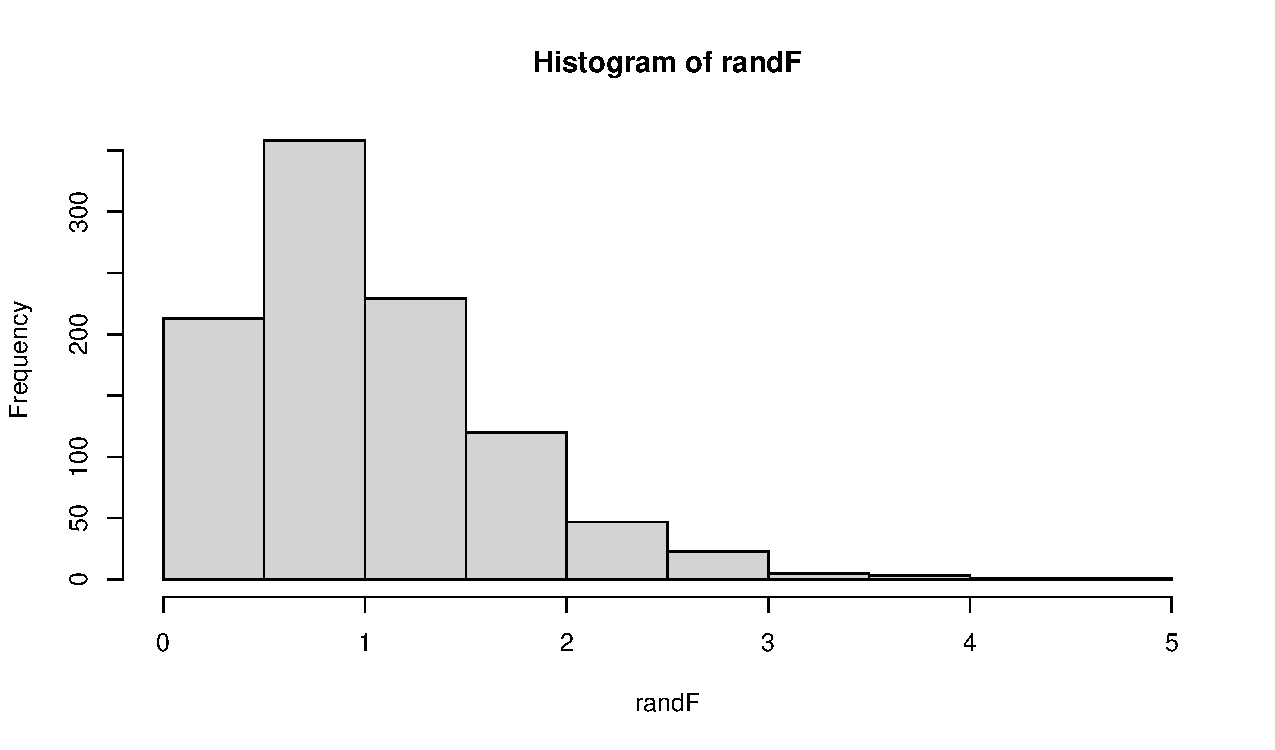
\includegraphics[width=\maxwidth]{figure/unnamed-chunk-35-1} 

}


\end{knitrout}
% \end{noindent}
\subsection*{The Logit Link and Odds Ratios}
\addcontentsline{toc}{subsection}{The Logit Link and Odds Ratios}
\begin{itemize}
      \item The \textcolor{Blue}{Logit link} is the canonical link for the Binomial (see Chapter 1).
      \item This leads us to a \textcolor{Blue}{Logistic Regression Model}:
            \[ \log*{\frac{\pi_i}{1-\pi_i}}=\Vector{x}_i^\top \Vector{\beta} \]
      \item Aside: The inverse of the logit function is called the expit function:
            \[ \logit{a}=\log*{\frac{a}{1-a}}=b\iff a=\frac{\exp{b}}{1+\exp{b}}=\expit{b} \]
      \item Next: What is the interpretation of the $ \Vector{\beta} $ parameters in this model?
\end{itemize}
\subsection*{Simple Logistic Regression}
\begin{itemize}
      \item Consider a simple case of a binomial outcome $ Y_i \sim \BIN{m_i,\pi_i} $ for $ i=0,1 $ and a single binary explanatory variable:
            \[ x_{i1}=\begin{cases*}
                        0 & group 0 \\
                        1 & group 1
                  \end{cases*} \]
      \item The simple logistic regression model equation is:
            \[ \log*{\frac{\pi_i}{1-\pi_i}}=\beta_0+\beta_1x_{i1} \]
      \item When $ x_{i1}=0 $ for $ i=0 $, the model becomes:
            \[ \log*{\frac{\pi_0}{1-\pi_0}}=\beta_0+\beta_1(0)=\beta_0 \]
      \item \textcolor{Blue}{$ \beta_0 = $ log odds of response for subjects with $ x_{i1}=0 $}.
      \item Now let's compare the model with $ x_{i1}=1 $ versus $ x_{i1}=0 $.
            \begin{table}[!htbp]
                  \centering
                  \begin{NiceTabular}{ccrl}
                        Group & $ (1,x_{i1})^\top $ & $ \eta_i $ & $ =\log[\big]{\pi_i/(1-\pi_i)} $\\
                        \midrule
                        1 & $ (1,1)^\top $ & $ \beta_0+\beta_1 $ & $ =\log[\big]{\pi_1/(1-\pi_1)} $\\
                        0 & $ (1,0)^\top $ & $ \beta_0 $ & $ =\log[\big]{\pi_0/(1-\pi_0)} $\\
                        \midrule
                        &&$ \beta_1 $ & $ =\log*{\frac{\pi_1/(1-\pi_1)}{\pi_0/(1-\pi_0)}} $
                  \end{NiceTabular}
            \end{table}
      \item We subtract line 2 from line 1 to isolate $ \beta_1 $ and find its interpretation.
      \item \textcolor{Blue}{$ \beta_1= $ log odds ratio of response for subjects with $ x_{i1}=1 $ vs $ x_{i1}=0 $}.
\end{itemize}
\subsection*{Logistic Regression Models for Prenatal Care Example}
\begin{itemize}
      \item \textcolor{Blue}{Response} $ = $ Fetal mortality
            \[ \textcolor{Blue}{Y_i \sim \BIN{m_i,\pi_i}}\qquad\text{$i=1,2,\ldots,n$ independently} \]
      \item \textcolor{Blue}{Explanatory Variables}:
            \begin{align*}
                  x_{i1} & =\begin{cases*}
                                  1 & Clinic A \\
                                  0 & Clinic B
                            \end{cases*}                                         \\
                  x_{i2} & =\begin{cases*}
                                  1 & Intensive level of care \\
                                  0 & Regular level of care   \\
                            \end{cases*}                           \\
                  x_{i3} & =x_{i1}x_{i2}=\begin{cases*}
                                               1 & Intensive level of care and Clinic A \\
                                               0 & Otherwise
                                         \end{cases*}
            \end{align*}
      \item We will use the context of this example to interpret regression parameters from
            multiple logistic regression models.
      \item See Section 2.4.2 for general interpretations.
\end{itemize}
\subsection*{Model 1: Clinic only model}
\[ \textcolor{Green}{\log*{\frac{\pi_i}{1-\pi_i}}=\beta_0+\beta_1x_{i1}} \]
\begin{table}[!htbp]
      \centering
      \begin{NiceTabular}{cccl}
            Clinic & Level of Care & $ (1,x_{i1})^\top $ & $ \log[\big]{\pi_i/(1-\pi_i)} $\\
            \midrule
            A & --- & $ (1,1)^\top $ & $ \beta_0+\beta_1 $\\
            B & --- & $ (1,0)^\top $ & $ \beta_0 $
      \end{NiceTabular}
      \caption{Clinic only model}
\end{table}
\begin{itemize}
      \item $ \beta_0 $ is the \textcolor{Blue}{log odds} of infant mortality for babies born to mothers treated at Clinic B.
      \item $ \beta_1 $ is the \textcolor{Blue}{log odds ratio} of mortality for babies born to mothers treated at Clinic A
            versus Clinic B.
\end{itemize}
\subsection*{Model 2: Main effects model}
\[ \textcolor{Green}{\log*{\frac{\pi_i}{1-\pi_i}}=\beta_0+\beta_1x_{i1}+\beta_2x_{i2}} \]
\begin{table}[!htbp]
      \centering
      \begin{NiceTabular}{cccl}
            Clinic & Level of Care & $ (1,x_{i1},x_{i2})^\top $ & $ \log[\big]{\pi_i/(1-\pi_i)} $\\
            \midrule
            A & Intensive & $ (1,1,1)^\top $ & $ \beta_0+\beta_1+\beta_2 $\\
            A & Regular & $ (1,1,0)^\top $ & $ \beta_0+\beta_1 $\\
            B & Intensive & $ (1,0,1)^\top $ & $ \beta_0+\beta_2 $\\
            B & Regular & $ (1,0,0)^\top $ & $ \beta_0 $
      \end{NiceTabular}
      \caption{Main effects model}
\end{table}
\begin{itemize}
      \item $ \beta_0 $ is the \textcolor{Blue}{log odds} of infant mortality for babies born to mothers treated at Clinic
            B with Regular care.
      \item $ \beta_1 $ is the \textcolor{Blue}{log odds ratio} of mortality for babies born to mothers treated at Clinic A
            versus Clinic B at the same level of care.
      \item $ \beta_2 $ is the \textcolor{Blue}{log odds ratio} of mortality for babies born to mothers treated with
            Intensive versus Regular care at the same clinic \textcolor{Red}{(*OR of interest*)}.
\end{itemize}
\subsection*{Model 3: Interaction model}
\[ \textcolor{Green}{\log*{\frac{\pi_i}{1-\pi_i}}=\beta_0+\beta_1x_{i1}+\beta_2x_{i2}+\beta_3x_{i3}} \]
\begin{table}[!htbp]
      \centering
      \begin{NiceTabular}{cccl}
            Clinic & Level of Care & $ (1,x_{i1},x_{i2},x_{i3})^\top $ & $ \log[\big]{\pi_i/(1-\pi_i)} $\\
            \midrule
            A & Intensive & $ (1,1,1,1)^\top $ & $ \beta_0+\beta_1+\beta_2+\beta_3 $\\
            A & Regular & $ (1,1,0,0)^\top $ & $ \beta_0+\beta_1 $\\
            B & Intensive & $ (1,0,1,0)^\top $ & $ \beta_0+\beta_2 $\\
            B & Regular & $ (1,0,0,0)^\top $ & $ \beta_0 $
      \end{NiceTabular}
      \caption{Interaction model}
\end{table}
\begin{itemize}
      \item $ \beta_1 $ is the \textcolor{Blue}{log odds ratio} of mortality for babies born to mothers treated at Clinic A
            versus Clinic B at Regular care.
      \item $ \beta_1+\beta_3 $ is the \textcolor{Blue}{log odds ratio} of mortality for babies born to mothers treated at
            Clinic A versus Clinic B at Intensive care.
      \item $ \beta_2 $ is the \textcolor{Blue}{log odds ratio} of mortality for babies born to mothers treated with
            Intensive versus Regular care at Clinic B.
      \item $ \beta_2+\beta_3 $ is the \textcolor{Blue}{log odds ratio} of mortality for babies born to mothers treated with
            Intensive versus Regular care at Clinic A.
      \item $ \beta_3 $ is a \textcolor{Blue}{difference is log ratio odds}.
      \item If $ \beta_3=0 $, then the association between mortality and level of care does not depend on Clinic.
      \item Equivalently, if $ \beta_3 = 0 $, then the association between mortality and Clinic does not depend on level of care.
\end{itemize}
\subsection*{Prediction from Logistic Regression}
\[ \logit{\pi_i}=\log*{\frac{\pi_i}{1-\pi_i}}=\eta_i\iff \pi_i=\frac{\exp{\eta_i}}{1+\exp{\eta_i}}=\expit{\eta_i} \]
\begin{itemize}
      \item Assume we have found $ \hat{\Vector{\beta}} $ using Fisher scoring (R \texttt{glm()} function).
      \item The fitted value for the \textcolor{Blue}{probability of response} $ \pi_i=\E{Y_i/m_i} $ for explanatory
            variable(s) $ \Vector{x}_i $ is:
            \[ \hat{\pi}_i=\hat{\pi}(\Vector{x}_i)=\frac{\exp{\Vector{x}_i^\top \hat{\Vector{\beta}}}}{1+\exp{\Vector{x}_i^\top \hat{\Vector{\beta}}}}=\expit{\Vector{x}_i^\top \hat{\Vector{\beta}}}  \]
      \item The \textcolor{Blue}{predicted number of responses} is: $ \hat{Y}_i=m_i\hat{\pi}_i $.
\end{itemize}
\subsection*{Logistic Regression Analysis of Prenatal Care Data}
\addcontentsline{toc}{subsection}{Logistic Regression Analysis of Prenatal Care Data}
\begin{itemize}
      \item \textcolor{Blue}{Previously}: Analysis using likelihood for $ 2\times 2 $ tables:
            \begin{table}[!htbp]
                  \centering
                  \begin{NiceTabular}{ll}
                        Odds Ratio (outcome = mortality) & Estimate and \qty{95}{\percent} CI\\
                        \midrule
                        Intensive vs Regular & $ 0.51\; (0.30,0.89) $\\
                        Intensive vs Regular at Clinic A & $ 0.80\; (0.37,1.73) $\\
                        Intensive vs Regular at Clinic B & $ 1.01\; (0.33,3.10) $\\
                        \midrule
                  \end{NiceTabular}
            \end{table}
      \item \textcolor{Blue}{Now}:
            \begin{enumerate}[1.]
                  \item Use \texttt{glm()} function in R to fit logistic regression models and estimate $ \hat{\Vector{\beta}} $.
                  \item Extract estimates $ \beta_k $ with $ \log{\text{OR}} $ interpretations.
                  \item Conduct hypothesis tests for $ \HN $: $ \beta_k=\beta_{k0} $.
                  \item Calculate \qty{95}{\percent} confidence intervals for $ \beta_k $ and $ \psi=\exp{\beta_k} $.
                  \item Try to find best fitting model with fewest parameters.
            \end{enumerate}
\end{itemize}
\subsection*{R Data and Code}
\begin{Example}{Data file \texttt{prenatal.dat}}
\begin{knitrout}
\definecolor{shadecolor}{rgb}{0.969, 0.969, 0.969}\color{fgcolor}\begin{kframe}
\begin{verbatim}
  clinic loc  y   m
1      0   0 34 231
2      0   1  4  27
3      1   0 12 188
4      1   1 16 309
\end{verbatim}
\end{kframe}
\end{knitrout}
\end{Example}
\begin{itemize}
      \item The first line contains the variable names/labels.
      \item We are using indicator variables for the explanatory variables.
            \begin{itemize}
                  \item $ x_{i1}=\texttt{clinic}=\Ind{\text{Clinic A}} $.
                  \item $ x_{i2}=\texttt{loc}=\Ind{\text{Intensive care}} $.
            \end{itemize}
      \item The response variable \texttt{y} is the number of events (deaths).
      \item \texttt{m} is the number of binomial trials (number of mothers).
\end{itemize}
% \begin{noindent}
\begin{knitrout}
\definecolor{shadecolor}{rgb}{0.969, 0.969, 0.969}\color{fgcolor}\begin{kframe}
\begin{alltt}
\hlcom{# R program for analysis of prenatal care data}
\hlstd{prenatal.dat} \hlkwb{<-} \hlkwd{read.table}\hlstd{(}\hlstr{"prenatal.dat"}\hlstd{,} \hlkwc{header} \hlstd{= T)}
\hlcom{# here we construct the response variable for the logistic}
\hlcom{# regression analysis}
\hlstd{prenatal.dat}\hlopt{$}\hlstd{resp} \hlkwb{<-} \hlkwd{cbind}\hlstd{(prenatal.dat}\hlopt{$}\hlstd{y, prenatal.dat}\hlopt{$}\hlstd{m} \hlopt{-} \hlstd{prenatal.dat}\hlopt{$}\hlstd{y)}
\hlstd{prenatal.dat}
\hlcom{# now we fit the model using the glm function and store the}
\hlcom{# result in 'model 1' we indicate 'resp' contains a}
\hlcom{# binomial response and that we are using the logistic link}
\hlcom{# function}
\hlstd{model1} \hlkwb{<-} \hlkwd{glm}\hlstd{(resp} \hlopt{~} \hlstd{loc,} \hlkwc{family} \hlstd{=} \hlkwd{binomial}\hlstd{(}\hlkwc{link} \hlstd{= logit),} \hlkwc{data} \hlstd{= prenatal.dat)}
\hlkwd{summary}\hlstd{(model1)}
\hlcom{# the 'names' function lists the contents of the object}
\hlcom{# 'model1' and following this statement we examine some of}
\hlcom{# the contents of these objects (try it)}
\hlkwd{names}\hlstd{(model1)}
\hlstd{model1}\hlopt{$}\hlstd{family}
\hlstd{model1}\hlopt{$}\hlstd{formula}
\hlstd{model1}\hlopt{$}\hlstd{coefficients}
\hlstd{model1}\hlopt{$}\hlstd{deviance}
\hlstd{model1}\hlopt{$}\hlstd{fitted.values}
\hlstd{model1}\hlopt{$}\hlstd{residuals}
\hlcom{# now we fit a model to examine the relationship between}
\hlcom{# level of care and mortality adjusting for clinic}
\hlstd{model2} \hlkwb{<-} \hlkwd{glm}\hlstd{(resp} \hlopt{~} \hlstd{clinic} \hlopt{+} \hlstd{loc,} \hlkwc{family} \hlstd{=} \hlkwd{binomial}\hlstd{(}\hlkwc{link} \hlstd{= logit),}
  \hlkwc{data} \hlstd{= prenatal.dat)}
\hlkwd{summary}\hlstd{(model2)}
\hlcom{# here we examine whether the association between loc and}
\hlcom{# mortality depends on the clinic}
\hlstd{model3} \hlkwb{<-} \hlkwd{glm}\hlstd{(resp} \hlopt{~} \hlstd{loc} \hlopt{+} \hlstd{clinic} \hlopt{+} \hlstd{loc} \hlopt{*} \hlstd{clinic,} \hlkwc{family} \hlstd{=} \hlkwd{binomial}\hlstd{(}\hlkwc{link} \hlstd{= logit),}
  \hlkwc{data} \hlstd{= prenatal.dat)}
\hlkwd{summary}\hlstd{(model3)}
\hlcom{# now we examine the marginal relationship between}
\hlcom{# mortality and clinic}
\hlstd{model4} \hlkwb{<-} \hlkwd{glm}\hlstd{(resp} \hlopt{~} \hlstd{clinic,} \hlkwc{family} \hlstd{=} \hlkwd{binomial}\hlstd{(}\hlkwc{link} \hlstd{= logit),}
  \hlkwc{data} \hlstd{= prenatal.dat)}
\hlkwd{summary}\hlstd{(model4)}
\end{alltt}
\end{kframe}
\end{knitrout}
% \end{noindent}
\subsection*{Selected R Output}
Print the augmented dataframe to see what the \textcolor{Blue}{\texttt{resp} variable} $ (Y_i,m_i-Y_i) $ looks like:
% \begin{noindent}
\begin{knitrout}
\definecolor{shadecolor}{rgb}{0.969, 0.969, 0.969}\color{fgcolor}\begin{kframe}
\begin{alltt}
\hlcom{# here we construct the response variable for the logistic}
\hlcom{# regression analysis}
\hlstd{prenatal.dat}\hlopt{$}\hlstd{resp} \hlkwb{<-} \hlkwd{cbind}\hlstd{(prenatal.dat}\hlopt{$}\hlstd{y, prenatal.dat}\hlopt{$}\hlstd{m} \hlopt{-} \hlstd{prenatal.dat}\hlopt{$}\hlstd{y)}
\hlstd{prenatal.dat}
\end{alltt}
\begin{verbatim}
  clinic loc  y   m resp.1 resp.2
1      0   0 34 231     34    197
2      0   1  4  27      4     23
3      1   0 12 188     12    176
4      1   1 16 309     16    293
\end{verbatim}
\end{kframe}
\end{knitrout}
% \end{noindent}
The \textcolor{Blue}{logistic regression} models are fit using the \texttt{glm} commands like:
% \begin{noindent}
\begin{knitrout}
\definecolor{shadecolor}{rgb}{0.969, 0.969, 0.969}\color{fgcolor}\begin{kframe}
\begin{alltt}
\hlcom{# now we fit the model using the glm function and store the}
\hlcom{# result in 'model 1' we indicate 'resp' contains a}
\hlcom{# binomial response and that we are using the logistic link}
\hlcom{# function}
\hlstd{model1} \hlkwb{<-} \hlkwd{glm}\hlstd{(resp} \hlopt{~} \hlstd{loc,} \hlkwc{family} \hlstd{=} \hlkwd{binomial}\hlstd{(}\hlkwc{link} \hlstd{= logit),} \hlkwc{data} \hlstd{= prenatal.dat)}
\hlkwd{summary}\hlstd{(model1)}
\end{alltt}
\end{kframe}
\end{knitrout}
% \end{noindent}
\subsection*{Fit of Model 1: Level of Care Model}
\[ \log*{\frac{\pi_i}{1-\pi_i}}=\beta_0+\beta_2x_{i2} \]
% \begin{noindent}
\begin{knitrout}
\definecolor{shadecolor}{rgb}{0.969, 0.969, 0.969}\color{fgcolor}\begin{kframe}
\begin{alltt}
\hlstd{model1} \hlkwb{<-} \hlkwd{glm}\hlstd{(resp} \hlopt{~} \hlstd{loc,} \hlkwc{family} \hlstd{=} \hlkwd{binomial}\hlstd{(}\hlkwc{link} \hlstd{= logit),} \hlkwc{data} \hlstd{= prenatal.dat)}
\hlkwd{summary}\hlstd{(model1)}\hlopt{$}\hlstd{coefficients}
\end{alltt}
\begin{verbatim}
              Estimate Std. Error    z value     Pr(>|z|)
(Intercept) -2.0929370  0.1562692 -13.393150 6.630754e-41
loc         -0.6670729  0.2785400  -2.394891 1.662530e-02
\end{verbatim}
\end{kframe}
\end{knitrout}
% \end{noindent}
\subsection*{Components of the \texttt{summary()} output for \texttt{glm} objects}
\begin{itemize}
      \item \textcolor{Blue}{\texttt{Estimate}}: the maximum likelihood estimates of the regression coefficients $ \hat{\beta}_k $.
      \item \textcolor{Blue}{\texttt{Std Error}}: estimated standard errors based on the inverse of the information.
            \[ \se{\hat{\beta}_k}=\sqrt{\bigl(\Matrix{I}^{-1}(\hat{\Vector{\beta}})\bigr)_{kk}}=\sqrt{I^{kk}(\hat{\Vector{\beta}})} \]
      \item \textcolor{Blue}{\texttt{z value}}: Wald-based test statistics for the hypothesis test:
            \begin{center}
                  $ \HN $: $ \beta_k=0 $ vs $ \HA $: $ \beta_k\ne 0 $.
            \end{center}
      \item \textcolor{Blue}{\texttt{Pr(>|z|)}}: $ p $-value for the above test.
\end{itemize}
\textcolor{Blue}{For this model}:
\begin{itemize}
      \item $ \beta_2 $ is the log odds ratio of mortality for babies born to mothers treated with
            Intensive versus Regular care.
            \[ \hat{\psi}=\exp{\hat{\beta}_2}=\exp{-0.6670729}=0.51 \]
\end{itemize}
\subsection*{Hypothesis test for $ \beta_k $}
\begin{itemize}
      \item We may wish to test:
            \begin{center}
                  $ \HN $: $ \beta_k=\beta_{k0} $ versus $ \HA $: $ \beta_k\ne \beta_{k0} $
            \end{center}
      \item The general \textcolor{Blue}{Wald Result} for scalar $ \beta_k $ is:
            \[ (\hat{\beta}_k-\beta_{k0})^2\bigl(I^{kk}(\hat{\Vector{\beta}})\bigr)^{-1} \sim \chi^2_1 \]
            equivalently $ \displaystyle \frac{\hat{\beta}_k-\beta_{k0}}{\se{\hat{\beta}_k}}\sim \N{0,1} $ where $ \se{\hat{\beta}_k}=\sqrt{I^{kk}(\hat{\Vector{\beta}})} $.
      \item And we can find the $ p $-value of this test using
            \[ p=2\Prob*{Z>\frac{\abs{\hat{\beta}_k-\beta_{k0}}}{\se{\hat{\beta}_k}}}\qquad\text{where $ Z \sim \N{0,1} $} \]
      \item The \texttt{summary()} output gives the test statistics and $p$-values for testing
            \begin{center}
                  \begin{center}
                        $ \HN $: $ \beta_k=0 $ vs $ \HA $: $ \beta_k\ne 0 $
                  \end{center}
            \end{center}
\end{itemize}
\subsection*{Hypothesis test for $ \beta_2 $ from Model 1: Level of Care Model}
% \begin{noindent}
\begin{knitrout}
\definecolor{shadecolor}{rgb}{0.969, 0.969, 0.969}\color{fgcolor}\begin{kframe}
\begin{alltt}
\hlkwd{summary}\hlstd{(model1)}\hlopt{$}\hlstd{coefficients}
\end{alltt}
\begin{verbatim}
              Estimate Std. Error    z value     Pr(>|z|)
(Intercept) -2.0929370  0.1562692 -13.393150 6.630754e-41
loc         -0.6670729  0.2785400  -2.394891 1.662530e-02
\end{verbatim}
\end{kframe}
\end{knitrout}
          % \end{noindent}
\begin{itemize}
      \item We wish to test:
            \begin{center}
                  $ \HN $: $ \beta_2=0 $ vs $ \HA $: $ \beta_2\ne 0 $
            \end{center}
      \item The Wald-based test statistic is:
            \[ z^\star=\frac{\hat{\beta}_2-0}{\se{\hat{\beta}_2}}=\frac{-0.6671}{0.2785}=-2.3949   \]
      \item And we can find the $ p $-value of this test using:
            \[ p=2\Prob{Z>\abs{-2.3949}}=0.0166<0.05 \]
      \item Therefore, we reject the null hypothesis that $ \beta_2=0 $.
      \item Equivalently, we reject the null hypothesis that $ \text{OR}=1 $.
\end{itemize}
\subsection*{Confidence Interval for the OR}
\begin{itemize}
      \item Calculate CI for $ \beta_k=\log{\psi} $ and then exponentiate.
      \item Recall the \textcolor{Blue}{Wald-based} confidence interval:
            \[ \hat{\beta}_k\pm 1.96\se{\hat{\beta}_k} \]
      \item The \textcolor{Blue}{\texttt{Std Error}} from the \texttt{summary()} output is the square root of the diagonal of
            the inverse of the Information matrix.
            % \begin{noindent}
\begin{knitrout}
\definecolor{shadecolor}{rgb}{0.969, 0.969, 0.969}\color{fgcolor}\begin{kframe}
\begin{alltt}
\hlkwd{summary}\hlstd{(model1)}\hlopt{$}\hlstd{coefficients}
\end{alltt}
\begin{verbatim}
              Estimate Std. Error    z value     Pr(>|z|)
(Intercept) -2.0929370  0.1562692 -13.393150 6.630754e-41
loc         -0.6670729  0.2785400  -2.394891 1.662530e-02
\end{verbatim}
\begin{alltt}
\hlkwd{summary}\hlstd{(model1)}\hlopt{$}\hlstd{cov.unscaled}  \hlcom{# The inverse of the Information Matrix}
\end{alltt}
\begin{verbatim}
            (Intercept)         loc
(Intercept)  0.02442007 -0.02442007
loc         -0.02442007  0.07758452
\end{verbatim}
\begin{alltt}
\hlkwd{sqrt}\hlstd{(}\hlkwd{diag}\hlstd{(}\hlkwd{summary}\hlstd{(model1)}\hlopt{$}\hlstd{cov.unscaled))}  \hlcom{# The se of the betas}
\end{alltt}
\begin{verbatim}
(Intercept)         loc 
  0.1562692   0.2785400 
\end{verbatim}
\end{kframe}
\end{knitrout}
    % \end{noindent}
\end{itemize}
\subsection*{Confidence Interval for $ \exp{\beta_2} $ from Model 1: Level of Care Model}
% \begin{noindent}
\begin{knitrout}
\definecolor{shadecolor}{rgb}{0.969, 0.969, 0.969}\color{fgcolor}\begin{kframe}
\begin{alltt}
\hlkwd{summary}\hlstd{(model1)}\hlopt{$}\hlstd{coefficients}
\end{alltt}
\begin{verbatim}
              Estimate Std. Error    z value     Pr(>|z|)
(Intercept) -2.0929370  0.1562692 -13.393150 6.630754e-41
loc         -0.6670729  0.2785400  -2.394891 1.662530e-02
\end{verbatim}
\end{kframe}
\end{knitrout}
% \end{noindent}
\begin{itemize}
      \item The \qty{95}{\percent} confidence interval for the OR is:
            \begin{align*}
                  \exp[\big]{\hat{\beta}_k\pm 1.96\se{\hat{\beta}_k}}
                   & =\exp{-0.6671\pm 1.96(0.2785)} \\
                   & =(\exp{-1.2130},\exp{-0.1211}) \\
                   & =(0.30,0.89)
            \end{align*}
      \item Note: The estimate and \qty{95}{\percent} confidence interval here match those found
            previously from the $ 2\times 2 $ table analysis.
\end{itemize}
\subsection*{Fit of Model 2: Main Effects Model}
\[ \textcolor{Green}{\log*{\frac{\pi_i}{1-\pi_i}}=\beta_0+\beta_1x_{i1}+\beta_2x_{i2}} \]
% \begin{noindent}
\begin{knitrout}
\definecolor{shadecolor}{rgb}{0.969, 0.969, 0.969}\color{fgcolor}\begin{kframe}
\begin{alltt}
\hlstd{model2} \hlkwb{<-} \hlkwd{glm}\hlstd{(resp} \hlopt{~} \hlstd{clinic} \hlopt{+} \hlstd{loc,} \hlkwc{family} \hlstd{=} \hlkwd{binomial}\hlstd{(}\hlkwc{link} \hlstd{= logit),}
  \hlkwc{data} \hlstd{= prenatal.dat)}
\hlkwd{summary}\hlstd{(model2)}\hlopt{$}\hlstd{coefficients}
\end{alltt}
\begin{verbatim}
              Estimate Std. Error    z value     Pr(>|z|)
(Intercept) -1.7410476  0.1784691 -9.7554560 1.748132e-22
clinic      -0.9862793  0.3089322 -3.1925427 1.410261e-03
loc         -0.1503053  0.3301670 -0.4552402 6.489365e-01
\end{verbatim}
\end{kframe}
\end{knitrout}
% \end{noindent}
\begin{itemize}
      \item \textcolor{Blue}{Odds Ratio for mortality for Intensive versus Regular care, controlling for clinic}:
            \[ \exp{\hat{\beta}_2}=\exp{-0.1503}=0.860 \]
\end{itemize}
\subsection*{Fit of Model 3: Interaction Model}
\[ \textcolor{Green}{\log*{\frac{\pi_i}{1-\pi_i}}=\beta_0+\beta_1x_{i1}+\beta_2x_{i2}+\beta_3x_{i3}} \]
% \begin{noindent}
\begin{knitrout}
\definecolor{shadecolor}{rgb}{0.969, 0.969, 0.969}\color{fgcolor}\begin{kframe}
\begin{alltt}
\hlstd{model3} \hlkwb{<-} \hlkwd{glm}\hlstd{(resp} \hlopt{~} \hlstd{loc} \hlopt{+} \hlstd{clinic} \hlopt{+} \hlstd{loc} \hlopt{*} \hlstd{clinic,} \hlkwc{family} \hlstd{=} \hlkwd{binomial}\hlstd{(}\hlkwc{link} \hlstd{= logit),}
  \hlkwc{data} \hlstd{= prenatal.dat)}
\hlkwd{summary}\hlstd{(model3)}\hlopt{$}\hlstd{coefficients}
\end{alltt}
\begin{verbatim}
                Estimate Std. Error     z value     Pr(>|z|)
(Intercept) -1.756843204  0.1857092 -9.46018403 3.074017e-21
loc          0.007643349  0.5726827  0.01334657 9.893513e-01
clinic      -0.928734141  0.3514300 -2.64272868 8.224091e-03
loc:clinic  -0.229649891  0.6949054 -0.33047646 7.410400e-01
\end{verbatim}
\end{kframe}
\end{knitrout}
% \end{noindent}
\subsection*{Interpretation of Model 3: Interaction Model}
\begin{table}[!htbp]
      \centering
      \begin{NiceTabular}{cccl}
            Clinic & Level of Care & $ (1,x_{i1},x_{i2},x_{i3})^\top $ & $ \log[\big]{\pi_i/(1-\pi_i)} $\\
            \midrule
            A & Intensive & $ (1,1,1,1)^\top $ & $ \beta_0+\beta_1+\beta_2+\beta_3 $\\
            A & Regular & $ (1,1,0,0)^\top $ & $ \beta_0+\beta_1 $\\
            B & Intensive & $ (1,0,1,0)^\top $ & $ \beta_0+\beta_2 $\\
            B & Regular & $ (1,0,0,0)^\top $ & $ \beta_0 $
      \end{NiceTabular}
\end{table}
\begin{itemize}
      \item \textcolor{Blue}{Odds Ratio for mortality for Intensive vs Regular care, Clinic A}:
            \[ \exp{\hat{\beta}_2+\hat{\beta}_3}=\exp{0.007643-0.229650}=0.80=\hat{\psi}_\text{A} \]
      \item \textcolor{Blue}{Odds Ratio for mortality for Intensive vs Regular care, Clinic B}:
            \[ \exp{\hat{\beta}_2}=\exp{0.007643}=1.01=\hat{\psi}_\text{B} \]
\end{itemize}
\subsection*{Fit of Model 4: Clinic Only Model}
\[ \textcolor{Green}{\log*{\frac{\pi_i}{1-\pi_i}}=\beta_0+\beta_1x_{i1}} \]
% \begin{noindent}
\begin{knitrout}
\definecolor{shadecolor}{rgb}{0.969, 0.969, 0.969}\color{fgcolor}\begin{kframe}
\begin{alltt}
\hlstd{model4} \hlkwb{<-} \hlkwd{glm}\hlstd{(resp} \hlopt{~} \hlstd{clinic,} \hlkwc{family} \hlstd{=} \hlkwd{binomial}\hlstd{(}\hlkwc{link} \hlstd{= logit),}
  \hlkwc{data} \hlstd{= prenatal.dat)}
\hlkwd{summary}\hlstd{(model4)}\hlopt{$}\hlstd{coefficients}
\end{alltt}
\begin{verbatim}
             Estimate Std. Error   z value     Pr(>|z|)
(Intercept) -1.756041  0.1756737 -9.996041 1.586117e-23
clinic      -1.062357  0.2621216 -4.052916 5.058308e-05
\end{verbatim}
\end{kframe}
\end{knitrout}
% \end{noindent}
\begin{itemize}
      \item \textcolor{Blue}{Odds Ratio for mortality in Clinic A versus Clinic B}:
            \[ \exp{\hat{\beta}_1}=\exp{-1.0624}=0.35 \]
\end{itemize}
\subsection*{Prenatal Care Wrap-up}
\begin{itemize}
      \item Model 4 provides the best fit to the data with the fewest parameters.
      \item However, the original research question was about the level of care therefore we
            select \textcolor{Blue}{Model 2} as our final model.
      \item Odds Ratio for mortality for Intensive versus Regular care, controlling for clinic:
            \[ \exp{\hat{\beta}_2}=\exp{-0.1503}=0.860 \]
      \item Exercises:
            \begin{enumerate}[1.]
                  \item Conduct a formal hypothesis test of $ \HN $: $ \beta_2=0 $ and confirm $ p $-value in the R output.
                  \item Show that the \qty{95}{\percent} confidence interval for the OR is $ (0.450,1.643) $.
                  \item Show that the Odds Ratio for mortality for Clinic B versus Clinic A, controlling for
                        level of care is:
                        \[ \exp{-\hat{\beta}_1}=\exp{0.9863}=2.68 \]
            \end{enumerate}
\end{itemize}

\section*{Topic 2c: Likelihood Ratio (Deviance) Tests}
\addcontentsline{toc}{section}{Topic 2c: Likelihood Ratio (Deviance) Tests}
\subsection*{Major Developments From Last Topic: Logistic Regression Models}
\begin{Regular}{Binomial GLM / Logistic Regression Model}
      $ Y_i \sim \BIN{m_i,\pi_i} $, $ i=1,\ldots,n $ independently with explanatory variables $ \Vector{x}_i $:
      \[ \log*{\frac{\pi_i}{1-\pi_i}}=\Vector{x}_i^\top \Vector{\beta} \]
\end{Regular}
\begin{itemize}
      \item \textcolor{Blue}{Estimation}: $ \hat{\Vector{\beta}} $ come from Fisher Scoring using R function \texttt{glm()}.
      \item \textcolor{Blue}{Interpretation}: $ \beta_k $ have log OR interpretations ($ k>0 $).
      \item \textcolor{Blue}{Hypothesis Tests} of $ \HN $: $ \beta_k=\beta_{k0} $ versus $ \HA $: $ \beta_k\ne \beta_{k0} $.
      \item \textcolor{Blue}{Confidence Intervals}: $ \hat{\beta}_k\pm z_{1-\alpha/2}\se{\hat{\beta}_k} $ where $ \se{\hat{\beta}_k}=\sqrt{I^{kk}(\hat{\Vector{\beta}})} $.
\end{itemize}
\subsection*{Topic 2c: Logistic Regression: Likelihood Ratio (Deviance) Tests}
\begin{enumerate}[1.]
      \item Likelihood for Binary (Logistic) Regression:
            \[ \ell(\Vector{\beta}\mid \Vector{y})=\sum_{i=1}^{n} \biggl(y_i(\Vector{x}_i^\top \Vector{\beta})-m_i\log[\big]{1+\exp{\Vector{x}_i^\top \Vector{\beta}}}\biggr) \]
      \item Likelihood Ratio Tests:
            \begin{align*}
                  -2\log[\big]{R(\theta)}          & =-2r(\theta)                  \sim \chi^2_1 &  & \text{Scalar $\theta$}                      \\
                  -2\log[\big]{R(\Vector{\theta})} & =-2r(\Vector{\theta})  \sim \chi^2_{n-p}    &  & \text{$ p $-dim Vector $ \Vector{\theta} $}
            \end{align*}
      \item Testing Nested Non-saturated Models:
            \begin{center}
                  $ \HN $: $ \beta_p=\cdots=\beta_{q-1}=0 $ vs $ \HA $: at least one of $ \beta_p,\ldots,\beta_{q-1}\ne 0 $
            \end{center}
\end{enumerate}
\subsection*{2.5 Likelihood for Binary (Logistic) Regression}
\addcontentsline{toc}{subsection}{Likelihood for Logistic Regression}
\begin{itemize}
      \item \textcolor{Blue}{Outcome/Response variable}: $ Y_i \sim \BIN{m_i,\pi_i} $, $ i=1,\ldots, n $.
            \begin{align*}
                  \mathcal{L}(\Vector{\pi}\mid \Vector{y}) & =\prod_{i=1}^n \pi_i^{y_i}(1-\pi_i)^{m_i-y_i}                     \\
                  \ell(\Vector{\pi}\mid \Vector{y})        & =\sum_{i=1}^{n} \bigl(y_i\log{\pi_i}+(m_i-y_i)\log{1-\pi_i}\bigr)
            \end{align*}
      \item \textcolor{Blue}{Explanatory variables}: $ \Vector{x}_i=(x_{i0},x_{i1},\ldots,x_{i(p-1)})^\top $.
      \item \textcolor{Blue}{Regression parameters}: $ \Vector{\beta}=(\beta_0,\beta_1,\ldots,\beta_{p-1})^\top $.
      \item \textcolor{Blue}{Link function}: logistic link
            \[ g(\pi_i)=\log*{\frac{\pi_i}{1-\pi_i}}=\Vector{x}_i^\top \Vector{\beta} \]
\end{itemize}
\subsection*{Likelihood for Logistic Regression}
\begin{itemize}
      \item Log likelihood for Binomial distribution:
            \[ \ell(\Vector{\pi}\mid \Vector{y})=\sum_{i=1}^{n} \Biggl(y_i\log*{\frac{\pi_i}{1-\pi_i}}+m_i\log{1-\pi_i}\Biggr) \]
      \item Using logit link we can reparameterize the log-likelihood in terms of $ \Vector{\beta} $:
            \[ \log*{\frac{\pi_i}{1-\pi_i}}=\Vector{x}_i^\top \Vector{\beta},\qquad \pi_i=\frac{\exp{\Vector{x}_i^\top \Vector{\beta}}}{1+\exp{\Vector{x}_i^\top \Vector{\beta}}}   \]
            \[ \log{1-\pi_i}=\log*{\frac{\exp{\Vector{x}_i^\top \Vector{\beta}}}{1+\exp{\Vector{x}_i^\top \Vector{\beta}}}}=\log*{\frac{1}{1+\exp{\Vector{x}_i^\top \Vector{\beta}}}}=-\log[\big]{1+\exp{\Vector{x}_i^\top \Vector{\beta}}} \]
      \item Log likelihood for logistic regression:
            \[ \ell(\Vector{\beta}\mid \Vector{y})=\sum_{i=1}^{n} \Bigl(y_i(\Vector{x}_i^\top \Vector{\beta})-m_i\log[\big]{1+\exp{\Vector{x}_i^\top \Vector{\beta}}}\Bigr) \]
      \item If $ \dim(\Vector{\beta})=p<n $, the model is said to be \textcolor{Blue}{unsaturated}.
      \item If $ p=n $, we have a \textcolor{Blue}{saturated} model.
      \item Maximize $ \ell(\Vector{\beta}\mid \Vector{y}) $ to obtain the MLE's $ \hat{\Vector{\beta}} $ (i.e., using Fisher Scoring in R \texttt{glm()}).
      \item Transform to get estimates $ \hat{\pi}_i=\expit{\Vector{x}_i^\top \hat{\Vector{\beta}}} $.
      \item For a saturated model, $ \expit{\Vector{x}_i^\top \hat{\Vector{\beta}}} $ will equal the Binomial MLE $ y_i/m_i $, and we will have $ m_i\hat{\pi}_i=y_i $ (i.e., a perfect fit).
\end{itemize}
\subsection*{Hypothesis Tests for Logistic Regression}
\begin{itemize}
      \item We want to ask: \textcolor{Red}{how good is the model?}
      \item How well do the $ m_i\hat{\pi}_i $ approximate the data $ y_i $?
      \item How much worse is the fit of a particular unsaturated model versus the saturated
            model?
      \item \textcolor{Blue}{Previously}: Wald-based tests of:
            \begin{center}
                  $ \HN $: $ \beta_k=\beta_{k0} $ versus $ \HA $: $ \beta_k\ne \beta_{k0} $.
            \end{center}
      \item \textcolor{Blue}{Today}: Likelihood Ratio based tests for:
            \begin{center}
                  $ \HN $: $ \beta_k=\beta_{k+1}=0 $ versus $ \HA $: $ \beta_k\ne 0 $ or $ \beta_{k+1}\ne 0 $.
            \end{center}
      \item This will allow us to test the overall fit of \textcolor{Green}{nested models}.
\end{itemize}
\subsection*{Likelihood Ratio Tests --- General Setting}
\addcontentsline{toc}{subsection}{Likelihood Ratio Tests}
\begin{itemize}
      \item Suppose $ \mathcal{L}(\Vector{\theta}) $ is the likelihood of a $ q $-dim parameter vector $ \Vector{\theta} $.
            \begin{itemize}
                  \item Let $ \tilde{\Vector{\theta}} $ be the $ q $-dim MLE (unconstrained/\textcolor{Blue}{saturated}, $ q=n $).
                  \item Let $ \hat{\Vector{\theta}} $ be the $ p $-dim MLE (constrained/\textcolor{Blue}{unsaturated}, $ p<q $).
            \end{itemize}
      \item $ \HN $: the unsaturated $ p $-dim model is adequate.
      \item $ \HA $: the $ p $-dim model is not adequate.
      \item Recall the \textcolor{Blue}{Likelihood Ratio result}. Under $ \HN $,
            \[ \textcolor{Blue}{-2\log[\big]{R(\Vector{\theta})}=-2\log*{\frac{\mathcal{L}(\hat{\Vector{\theta}})}{\mathcal{L}(\tilde{\Vector{\theta}})}}=-2\bigl(\ell(\hat{\Vector{\theta}})-\ell(\tilde{\Vector{\theta}})\bigr) \sim \chi^2_{q-p}} \]
      \item This is often referred to as the \textcolor{Blue}{Deviance}: $ D=-2\log[\big]{R(\Vector{\theta})} $.
      \item Reject $ \HN $ at significance level $ \theta $ if:
            \[ \Prob[\Big]{\chi^2_{q-p}>-2\log[\big]{R(\Vector{\theta})}}<\alpha \]
\end{itemize}
\subsection*{Likelihood Ratio Tests --- Logistic Regression}
\begin{itemize}
      \item \textcolor{Blue}{Saturated} model MLEs: $ \tilde{\pi}_i=y_i/m_i $, $ i=1,\ldots,n $.
      \item \textcolor{Blue}{Unsaturated} model MLEs: $ \hat{\pi}=\expit{\Vector{x}_i^\top \hat{\Vector{\beta}}} $.
            \begin{itemize}
                  \item Regression models are a way of imposing constraints on the estimation of $ \Vector{\pi} $ (through $ p $-dim $ \Vector{\beta} $).
            \end{itemize}
      \item $ \HN $: The $ p $-dim model $ \logit{\pi_i}=\Vector{x}_i^\top \Vector{\beta} $ is adequate.
      \item $ \HA $: The $ p $-dim model is not adequate compared to the $n$-dim saturated model.
      \item For the binomial with logit link the \textcolor{Blue}{LR/Deviance} test statistic is:
            \begin{align*}
                  D
                   & =-2\bigl(\ell(\hat{\Vector{\pi}})-\ell(\tilde{\Vector{\pi}})\bigr)                                                                                                                      \\
                   & =2\bigl(\ell(\tilde{\Vector{\pi}})-\ell(\hat{\Vector{\pi}})\bigr)                                                                                                                       \\
                   & =2\biggl[\sum_{i=1}^{n} \bigl(y_i\log{\tilde{\pi}_i}+(m_i-y_i)\log{1-\tilde{\pi}_i}\bigr)-\sum_{i=1}^{n} \bigl(y_i\log{\hat{\pi}_i}+(m_i-y_i)\log{1-\hat{\pi}_i}\bigr) \biggr]          \\
                   & =2\Biggl[\sum_{i=1}^{n} \Biggl(y_i\log*{\frac{y_i}{m_i}}+(m_i-y_i)\log*{\frac{m_i-y_i}{m_i}}\Biggr)-\sum_{i=1}^{n} \bigl(y_i\log{\hat{\pi}_i}+(m_i-y_i)\log{1-\hat{\pi}_i}\bigr)\Biggr] \\
                   & =2\Biggl[\sum_{i=1}^{n} \Biggl(y_i\log*{\frac{y_i}{m_i\hat{\pi}_i}}+(m_i-y_i)\log*{\frac{m_i-y_i}{m_i(1-\hat{\pi}_i)}}\Biggr)\Biggr]
            \end{align*}
      \item \textcolor{Blue}{Aside}: Note that $ D $ has the general form: $ D=2\sum\sum O_{ij}\log*{\frac{O_{jj}}{E_{ij}}} $.
\end{itemize}
\subsection*{Likelihood Ratio Tests --- Logistic Regression}
\begin{itemize}
      \item We expect $ D \sim \chi^2_{n-p} $ under $ \HN $.
            \begin{itemize}
                  \item Unfortunately, this is not a good approximation.
                  \item Approximation is much better for tested nested unsaturated models though.
            \end{itemize}
      \item In R, the $ D $ is reported as the \textcolor{Blue}{\texttt{Residual Deviance}}.
            % \begin{noindent}
\begin{knitrout}
\definecolor{shadecolor}{rgb}{0.969, 0.969, 0.969}\color{fgcolor}\begin{kframe}
\begin{alltt}
\hlstd{model3}\hlopt{$}\hlstd{deviance}
\end{alltt}
\begin{verbatim}
[1] -4.352074e-14
\end{verbatim}
\begin{alltt}
\hlstd{model4}\hlopt{$}\hlstd{deviance}
\end{alltt}
\begin{verbatim}
[1] 0.3148411
\end{verbatim}
\end{kframe}
\end{knitrout}
            % \end{noindent}
      \item $ \HN $: Model 4 is adequate, $ \HA $: Model 4 is not adequate compared to Model 3.
            \[ p=\Prob{\chi^2_{2}>0.3148}=0.85 \]
      \item Therefore do not reject the null hypothesis that Model 4 (Clinic only) is adequate.
\end{itemize}
\subsection*{Pearson Statistic --- Logistic Regression}
\begin{itemize}
      \item The \textcolor{Blue}{Pearson statistic} is another statistic one can use for assessing ``overall'' fit of a model.
            \[ \textcolor{Blue}{P=\sum_{i=1}^{n} \frac{(y_i-m_i\hat{\pi}_i)^2}{m_i\hat{\pi}_i(1-\hat{\pi}_i)}}  \]
      \item As with $ D $, $ P \sim \chi^2_{n-p} $ under $ \HN $: the model provides a reasonable fit to the data.
      \item Note: $ P $ has the general form $ P=\sum \frac{(O_i-E_i)^2}{V_i} $.
      \item The $ \chi^2 $ approximation is a bit better than for deviance statistics.
      \item Both are poor if sample size ($ m_i $) are small though.
\end{itemize}
\subsection*{2.6 Testing Nested Non-saturated Models}
\addcontentsline{toc}{subsection}{Testing Nested Models}
\begin{itemize}
      \item The previous LR/Deviance test was for an unsaturated model vs a saturated model.
      \item Now consider two unsaturated models and one saturated model ($ p<q<n $).
            \begin{align*}
                  \logit{\pi_i} & =\beta_0+\beta_1x_{i1}+\cdots+\beta_{p-1}x_{i(p-1)}\tag*{(1)}\label{2.6M1}                                                           \\
                  \logit{\pi_i} & =\beta_0+\beta_1x_{i1}+\cdots+\beta_{p-1}x_{i(p-1)}+\cdots+\beta_{q-1}x_{i(q-1)}\tag*{(2)}\label{2.6M2}                              \\
                  \logit{\pi_i} & =\beta_0+\beta_1x_{i1}+\cdots+\beta_{p-1}x_{i(p-1)}+\cdots+\beta_{q-1}x_{i(q-1)}+\cdots+\beta_{n-1}x_{i(n-1)}\tag*{(3)}\label{2.6M3}
            \end{align*}
      \item Model~\ref{2.6M1} is \textcolor{Blue}{nested} within Model~\ref{2.6M2}.
      \item $ \HN $: The $ p $-dim Model~\ref{2.6M1} fits the data as well as Model~\ref{2.6M2}.
            \begin{itemize}
                  \item $ \HN $: $ \beta_p=\cdots=\beta_{q-1}=0 $.
            \end{itemize}
      \item $ \HA $: Model~\ref{2.6M1} is inadequate compared to Model~\ref{2.6M2}.
            \begin{itemize}
                  \item $ \HA $: at least one of $ \beta_p,\ldots,\beta_{q-1}\ne 0 $.
            \end{itemize}
\end{itemize}
\subsection*{Testing Nested Non-saturated Models}
\begin{table}[!htbp]
      \centering
      \begin{NiceTabular}{lcc}
            \textcolor{Blue}{Model} & \textcolor{Blue}{Dimension} & \textcolor{Blue}{MLEs}\\
            \midrule
            \ref{2.6M1} Reduced model & $ p $ & $ \hat{\pi}_i $\\
            \ref{2.6M2} Full model & $ q $ & $ \tilde{\pi}_i $\\
            \ref{2.6M3} Saturated model & $ n $ & $ \tilde{\tilde{\pi}_i} $\\
            \bottomrule
      \end{NiceTabular}
\end{table}
\begin{itemize}
      \item Previously, found the LR/Deviance test vs saturated models.
      \item LR/Deviance test of~\ref{2.6M1} vs~\ref{2.6M3}:
            \[ \textcolor{Blue}{D_0=-2\bigl(\ell(\hat{\Vector{\pi}})-\ell(\tilde{\tilde{\Vector{\pi}}})\bigr)\sim \chi^2_{n-p}} \]
      \item LR/Deviance test of~\ref{2.6M2} vs~\ref{2.6M3}:
            \[ \textcolor{Blue}{D_\text{A}=-2\bigl(\ell(\tilde{\Vector{\pi}})-\ell(\tilde{\tilde{\Vector{\pi}}})\bigr)\sim \chi^2_{n-q}} \]
      \item Now we wish to conduct an LR/Deviance test of~\ref{2.6M1} vs~\ref{2.6M2}:
            \begin{align*}
                  \Delta D
                   & =-2\bigl(\ell(\hat{\Vector{\pi}})-\ell(\tilde{\Vector{\pi}})\bigr)                                                                                    \\
                   & =-2\bigl(\ell(\hat{\Vector{\pi}})-\ell(\tilde{\tilde{\Vector{\pi}}})\bigr)+2\bigl(\ell(\tilde{\Vector{\pi}})-\ell(\tilde{\tilde{\Vector{\pi}}})\bigr) \\
                   & =\textcolor{Blue}{D_0-D_\text{A}}
            \end{align*}
      \item Fact: If $ X_i \sim \chi^2_{r_i} $, then $ X_1+X_2 \sim \chi^2_{r_1+r_2} $.
      \item Therefore, under $ \HN $: $ \Delta D \sim \chi^2_{q-p} $.
            \begin{itemize}
                  \item This approximation is much better than when testing an unsaturated model versus
                        the saturated model.
            \end{itemize}
      \item If $ p=\Prob{\chi^2_{q-p}>\Delta D}<\alpha $ then reject $ \HN $: This implies:
            \begin{itemize}
                  \item Reduced model does not fit the data as well as Full model.
                  \item One or more of $ x_{ip},\ldots,x_{i(q-1)} $ is important (i.e., associated with the outcome).
            \end{itemize}
\end{itemize}
\subsection*{Testing Non-Saturated Models in Prenatal Care Example}
\begin{itemize}
      \item Summary of Deviance (``\texttt{Residual deviance}'') from R output:
            \begin{table}[!htbp]
                  \centering
                  \begin{NiceTabular}{cllc}
                        Model & Variables & Deviance & Parameters\\
                        \midrule
                        1 & \texttt{loc} & $10.81438$ & 2\\
                        2 & \texttt{clinic + loc} & $0.1069281$ & 3\\
                        3 & \texttt{clinic + loc + loc*clinic} & $\approx 0$ & 4\\
                        4 & \texttt{clinic} & $0.3148411$ & 2
                  \end{NiceTabular}
            \end{table}
      \item Is level of care associated with fetal mortality?
            \begin{center}
                  $ \HN $: $ \beta_2=0 $ versus $ \HA $: $ \beta_2\ne 0 $
            \end{center}
            % \begin{noindent}
\begin{knitrout}
\definecolor{shadecolor}{rgb}{0.969, 0.969, 0.969}\color{fgcolor}\begin{kframe}
\begin{alltt}
\hlcom{# Deviance/LR test H_0: Model 4 is adequate compared to}
\hlcom{# Model 2}
\hlstd{model4}\hlopt{$}\hlstd{deviance} \hlopt{-} \hlstd{model2}\hlopt{$}\hlstd{deviance}
\end{alltt}
\begin{verbatim}
[1] 0.207913
\end{verbatim}
\begin{alltt}
\hlnum{1} \hlopt{-} \hlkwd{pchisq}\hlstd{(model4}\hlopt{$}\hlstd{deviance} \hlopt{-} \hlstd{model2}\hlopt{$}\hlstd{deviance, model4}\hlopt{$}\hlstd{df.residual} \hlopt{-}
  \hlstd{model2}\hlopt{$}\hlstd{df.residual)}
\end{alltt}
\begin{verbatim}
[1] 0.6484081
\end{verbatim}
\begin{alltt}
\hlcom{# Reprint the fitted Model 2: Main Effects Only model}
\hlstd{model2} \hlkwb{<-} \hlkwd{glm}\hlstd{(resp} \hlopt{~} \hlstd{clinic} \hlopt{+} \hlstd{loc,} \hlkwc{family} \hlstd{=} \hlkwd{binomial}\hlstd{(}\hlkwc{link} \hlstd{= logit),}
  \hlkwc{data} \hlstd{= prenatal.dat)}
\hlkwd{summary}\hlstd{(model2)}
\end{alltt}
\begin{verbatim}

Call:
glm(formula = resp ~ clinic + loc, family = binomial(link = logit), 
    data = prenatal.dat)

Deviance Residuals: 
       1         2         3         4  
-0.08521   0.25805   0.13909  -0.11719  

Coefficients:
            Estimate Std. Error z value Pr(>|z|)    
(Intercept)  -1.7410     0.1785  -9.755  < 2e-16 ***
clinic       -0.9863     0.3089  -3.193  0.00141 ** 
loc          -0.1503     0.3302  -0.455  0.64894    
---
Signif. codes:  0 '***' 0.001 '**' 0.01 '*' 0.05 '.' 0.1 ' ' 1

(Dispersion parameter for binomial family taken to be 1)

    Null deviance: 16.91763  on 3  degrees of freedom
Residual deviance:  0.10693  on 1  degrees of freedom
AIC: 23.262

Number of Fisher Scoring iterations: 3
\end{verbatim}
\end{kframe}
\end{knitrout}
            % \end{noindent}
\end{itemize}
\subsection*{Summary: Likelihood Ratio (Deviance) Tests for Logistic Regression}
\begin{itemize}
      \item \textcolor{Blue}{(log) Relative Likelihood Result}: $ D=-2\log[\big]{R(\Vector{\theta})}=-2r(\Vector{\theta})\sim \chi^2_{n-p} $.
      \item For the binomial with logit link the \textcolor{Blue}{LR/Deviance} test statistic is:
            \[ D=2\Biggl[\sum_{i=1}^{n} \Biggl(y_i\log*{\frac{y_i}{m_i\hat{\pi}_i}}+(m_i-y_i)\log*{\frac{m_i-y_i}{m_i(1-\hat{\pi}_i)}}\Biggr)\Biggr] \]
      \item This is reported as the ``\texttt{Residual Deviance}'' in R \texttt{glm} summary output.
      \item Used to test the fit of nested non-saturated models $ (q>p) $:
            \[ \logit{\pi_i} =\beta_0+\beta_1x_{i1}+\cdots+\beta_{p-1}x_{i(p-1)}+\cdots+\beta_{q-1}x_{i(q-1)} \]
            \begin{itemize}
                  \item $ \HN $: $ \beta_p=\cdots=\beta_{q-1}=0 $.
                  \item $ \HA $: at least one of $ \beta_p,\ldots,\beta_{q-1}\ne 0 $.
            \end{itemize}
      \item Test statistic: $ \Delta D \sim \chi^2_{q-p} $ and $ p\text{-value}=\Prob{\chi^2_{q-p}>\Delta D} $.
\end{itemize}

\makeheading{Week 5}{\daterange{2021-10-04}{2021-10-08}}
\section*{Topic 2d: Logistic Regression: Residuals \& CIs}
\addcontentsline{toc}{section}{Topic 2d: Logistic Regression: Residuals \& Confidence Intervals}
\begin{Regular}{Binomial GLM / Logistic Regression Model}
      $ Y_i \sim \BIN{m_i,\pi_i} $, $ i=1,\ldots,n $ independently with explanatory variables $ \Vector{x}_i $:
      \[ \log*{\frac{\pi_i}{1-\pi_i}}=\Vector{x}_i^\top \Vector{\beta} \]
\end{Regular}
\begin{itemize}
      \item \textcolor{Blue}{Estimation}: $ \hat{\Vector{\beta}} $ come from Fisher scoring using R function \texttt{glm()}.
      \item \textcolor{Blue}{Interpretation}: $ \beta_k $ have log OR interpretations ($ k>0 $).
      \item Wald based \textcolor{Blue}{Hypothesis Tests} of $ \HN $: $ \beta_k=\beta_{k0} $ versus $ \HA $: $ \beta_k\ne \beta_{k0} $.
      \item \textcolor{Blue}{Confidence Intervals}: $ \hat{\beta}_k\pm z_{1-\alpha/2}\se{\hat{\beta}_k} $ where $ \se{\hat{\beta}_k}=\sqrt{I^{kk}(\hat{\Vector{\beta}})} $.
      \item Deviance/LR based \textcolor{Blue}{Hypothesis Tests} for nested models:
            \begin{center}
                  $ \HN $: $ \beta_p=\cdots=\beta_{q-1}=0 $ vs $ \HA $: at least one of $ \beta_p,\ldots,\beta_{q-1}\ne 0 $
            \end{center}
            using $ \Delta D=D_0-D_\text{A} \sim \chi^2_{q-p} $ under $ \HN $.
\end{itemize}
\subsection*{Topic 2d: Logistic Regression: Residuals \& Confidence Intervals}
\begin{enumerate}
      \item Residuals for Binomial Data --- \textcolor{Blue}{Deviance Residuals}:
            \[ r_i^D=\sign{y_i-m_i\hat{\pi}_i}\sqrt{\abs{d_i}} \]
      \item \textcolor{Green}{Neuroblastoma Example}:
            \begin{itemize}
                  \item Categorical explanatory variables: use of dummy variables.
                  \item Residual plots using Deviance Residuals.
                  \item Finding requested Odds Ratios.
            \end{itemize}
      \item \textcolor{Blue}{Confidence Intervals} for non-linear functions of $ \eta_i $:
            \begin{itemize}
                  \item How to get a CI for $ \exp{\beta_2-\beta_1} $ or $ \pi_i=\expit{\Vector{x}_i^\top \Vector{\beta}} $.
            \end{itemize}
\end{enumerate}
\subsection*{Residuals for Normal Linear Regression Models}
\addcontentsline{toc}{subsection}{Residuals for Normal Linear Regression Models}
\begin{itemize}
      \item The \textcolor{Blue}{raw residuals} were:
            \[ r_i=y_i-\hat{\mu}_i \]
      \item The \textcolor{Blue}{standardized residuals} were:
            \[ d_i=\frac{(y_i-\hat{\mu}_i)}{\hat{\sigma}\sqrt{1-h_{ii}}}\sim t_{n-p}\to \N{0,1}  \]
      \item The overall fit of the model and appropriateness of its underlying assumptions can
            be assessed using various types of \textcolor{Blue}{Residual Plots}. For example:
            \begin{itemize}
                  \item Residuals versus covariate $ x_j $ (checks linearity assumption).
                  \item Residuals versus fitted values $ \hat{\mu}_i $ (check normality and constant variance).
                  \item Normal QQ (quantile-quantile) plots of residuals (checks normality).
            \end{itemize}
\end{itemize}
\subsection*{2.7 Residuals for Binomial Data --- Deviance Residuals}
\begin{itemize}
      \item Recall the \textcolor{Blue}{LR/Deviance} test statistic:
            \begin{align*}
                  D
                   & =2\Biggl[\sum_{i=1}^{n} \Biggl(y_i\log*{\frac{y_i}{m_i\hat{\pi}_i}}+(m_i-y_i)\log*{\frac{m_i-y_i}{m_i(1-\hat{\pi}_i)}}\Biggr)\Biggr] \\
                   & =\sum_{i=1}^{n} d_i
            \end{align*}
      \item Define the \textcolor{Red}{Deviance Residuals} to be:
            \[ r_i^D=\sign{y_i-m_i\hat{\pi}_i}\sqrt{\abs{d_i}} \]
      \item Under $ \HN $: the model is adequate,
            \[ \sum_{i=1}^{n} d_i \sim \chi^2_{n-p}\implies r_i^D \sim \N{0,1} \]
      \item Use the plots of the deviance residuals to assess whether the $ r_i^D $ looks like independent $ \N{0,1} $ observations.
\end{itemize}
\subsection*{Residuals for Binomial Data --- Pearson Residuals}
\begin{itemize}
      \item Define the \textcolor{Red}{Pearson Residuals} to be:
            \[ \textcolor{Blue}{r_i^P=\frac{y_i-m_i\hat{\pi}_i}{\sqrt{m_i\hat{\pi}_i(1-\hat{\pi}_i)}}} \]
      \item Under $ \HN $: the model is adequate,
            $ r_i^P \sim \N{0,1} $.
      \item Note: if $ m_i\hat{\pi}_i<5 $ for one or more $ i $, we should be concerned about the validity of
            the approximation ($ \chi^2 $ or $ \N{0,1} $) and hence your conclusions (the same holds for $ m_i(1-\hat{\pi}_i) $).
\end{itemize}
\subsection*{2.8 Estimation of Prognosis for Children with Neuroblastoma}
\addcontentsline{toc}{subsection}{Neuroblastoma Example}
\begin{Example}{}
      \textbf{Purpose of Study}: To investigate the relationship between the probability of surviving
      2 years free of disease following diagnosis and treatment for neuroblastoma, and age at
      diagnosis and stage of disease at diagnosis.
      \begin{center}
            \begin{NiceTabular}{cccccc}
                  \toprule
                  &\multicolumn{5}{c}{Stage}\\
                  \midrule
                  Age (months) & I & II & III & IV & V\\
                  \midrule
                  0-11 & $ 11/12 $ & $ 15/16 $ & $ 2/4 $ & $ 5/18 $ & $ 18/19 $\\
                  12-23 & $ 3/4 $ & $ 3/7 $ & $ 5/8 $ & $ 0/25 $ & $ 1/3 $\\
                  24+ & $ 4/5 $ & $ 4/12 $ & $ 3/15 $ & $ 3/93 $ & $ 2/5 $\\
                  \bottomrule
            \end{NiceTabular}
      \end{center}
      Cell entries are of the form $y/m$ with $y$ representing the number of patients surviving 2
      years, and $m$ representing the number of patients in that age-stage combination at the
      start of the study.
\end{Example}
As an initial look at the data, consider the marginal distributions.
\begin{table}[!htbp]
      \centering
      \begin{NiceTabular}{cccccc|c}
            \toprule
            &\multicolumn{5}{c}{Stage}\\
            \midrule
            Age (months) & I & II & III & IV & V & Total\\
            \midrule
            0-11 & $ 11/12 $ & $ 15/16 $ & $ 2/4 $ & $ 5/18 $ & $ 18/19 $ & $ 51/69 $\\
            12-23 & $ 3/4 $ & $ 3/7 $ & $ 5/8 $ & $ 0/25 $ & $ 1/3 $ & $ 12/47 $\\
            24+ & $ 4/5 $ & $ 4/12 $ & $ 3/15 $ & $ 3/93 $ & $ 2/5 $ & $ 16/130 $\\
            \midrule
            Total & $ 18/21 $ & $ 22/35 $ & $ 10/27 $ & $ 8/136 $ & $ 21/27 $ & $ 79/246 $\\
            \bottomrule
      \end{NiceTabular}
\end{table}
\subsection*{Setting up the Regression Models}
\begin{itemize}
      \item \textcolor{Blue}{Outcome}: Let $Y_i$ be the number of children in group $i$ who survived 2 years out of
            $m_i$ total children in group $i$. Assume $ Y_i \sim \BIN{m_i,\pi_i} $ independently $ i=1,\ldots,15 $.
      \item \textcolor{Blue}{Explanatory variables}: Use dummy variables to represent Age and Stage levels:
            \[ \begin{array}{lll}
                        x_{i1}  = \begin{cases*}
                                        1 & if age 12-23 months \\
                                        0 & o.w.
                                  \end{cases*} &
                        x_{i2}  = \begin{cases*}
                                        1 & if age 24+ months \\
                                        0 & o.w.
                                  \end{cases*}   &
                        x_{i3} = \begin{cases*}
                                       1 & stage II \\
                                       0 & o.w.
                                 \end{cases*}            \\
                        x_{i4}  = \begin{cases*}
                                        1 & if stage III \\
                                        0 & o.w.
                                  \end{cases*}   &
                        x_{i5}  = \begin{cases*}
                                        1 & if stage IV \\
                                        0 & o.w.
                                  \end{cases*}   &
                        x_{i6}  = \begin{cases*}
                                        1 & if stage V \\
                                        0 & o.w.
                                  \end{cases*}
                  \end{array} \]
      \item Now consider the models:
            \begin{enumerate}[1.]
                  \item \textcolor{Green}{Age \& Stage}:
                        \[ \logit{\pi_i}=\beta_0+\beta_1x_{i1}+\beta_2x_{i2}+\beta_3x_{i3}+\beta_4x_{i4}+\beta_5x_{i5}+\beta_6x_{i6} \]
                  \item \textcolor{Green}{Age only}:
                        \[ \logit{\pi_i}=\beta_0+\beta_1x_{i1}+\beta_2x_{i2} \]
                  \item \textcolor{Green}{Stage only}:
                        \[ \logit{\pi_i}=\beta_0+\beta_3x_{i3}+\beta_4x_{i4}+\beta_5x_{i5}+\beta_6x_{i6} \]
            \end{enumerate}
\end{itemize}
\subsection*{R Data and Code}
\begin{Example}{Data file \texttt{neuro.dat}}
\begin{knitrout}
\definecolor{shadecolor}{rgb}{0.969, 0.969, 0.969}\color{fgcolor}\begin{kframe}
\begin{verbatim}
   age stage  y  m
1    1     1 11 12
2    1     2 15 16
3    1     3  2  4
4    1     4  5 18
5    1     5 18 19
6    2     1  3  4
7    2     2  3  7
8    2     3  5  8
9    2     4  0 25
10   2     5  1  3
11   3     1  4  5
12   3     2  4 12
13   3     3  3 15
14   3     4  3 93
15   3     5  2  5
\end{verbatim}
\end{kframe}
\end{knitrout}
\end{Example}
\begin{itemize}
      \item First line contains the variable labels.
      \item $ 15 $ observations.
      \item Recall \textbf{age} and \textbf{stage} are categorical (ordinal) variables, so we will have to compute the indicator variables in the R program.
\end{itemize}
% \begin{noindent}
\begin{knitrout}
\definecolor{shadecolor}{rgb}{0.969, 0.969, 0.969}\color{fgcolor}\begin{kframe}
\begin{alltt}
\hlcom{# Read in the Neuroblastoma dataset}
\hlstd{neuro.dat} \hlkwb{=} \hlkwd{read.table}\hlstd{(}\hlstr{"neuro.dat"}\hlstd{,} \hlkwc{header} \hlstd{= T)}
\hlcom{# here we create indicator variables for age and stage}
\hlstd{neuro.dat}\hlopt{$}\hlstd{agef} \hlkwb{=} \hlkwd{factor}\hlstd{(neuro.dat}\hlopt{$}\hlstd{age)}
\hlstd{neuro.dat}\hlopt{$}\hlstd{stagef} \hlkwb{=} \hlkwd{factor}\hlstd{(neuro.dat}\hlopt{$}\hlstd{stage)}
\hlcom{# here we construct the response variable for logistic}
\hlcom{# regression: (y, m-y)}
\hlstd{neuro.dat}\hlopt{$}\hlstd{resp} \hlkwb{=} \hlkwd{cbind}\hlstd{(neuro.dat}\hlopt{$}\hlstd{y, neuro.dat}\hlopt{$}\hlstd{m} \hlopt{-} \hlstd{neuro.dat}\hlopt{$}\hlstd{y)}
\hlstd{neuro.dat}
\hlcom{# here we fit the model with age and stage and print out}
\hlcom{# summary statistics}
\hlstd{model1} \hlkwb{=} \hlkwd{glm}\hlstd{(resp} \hlopt{~} \hlstd{agef} \hlopt{+} \hlstd{stagef,} \hlkwc{family} \hlstd{=} \hlkwd{binomial}\hlstd{(}\hlkwc{link} \hlstd{= logit),}
  \hlkwc{data} \hlstd{= neuro.dat)}
\hlkwd{summary}\hlstd{(model1)}
\hlkwd{summary}\hlstd{(model1,} \hlkwc{corr} \hlstd{= T)}\hlopt{$}\hlstd{correlation}
\hlcom{# record deviance residuals (rd1), linear predcitor (lp1),}
\hlcom{# and fitted values (fv1)}
\hlstd{rd1} \hlkwb{=} \hlkwd{residuals.glm}\hlstd{(model1,} \hlstr{"deviance"}\hlstd{)}
\hlstd{lp1} \hlkwb{=} \hlstd{model1}\hlopt{$}\hlstd{linear.predictors}
\hlstd{fv1} \hlkwb{=} \hlstd{model1}\hlopt{$}\hlstd{fitted.values}
\hlcom{# here we compute the Pearson residual as an exercise}
\hlstd{rp1} \hlkwb{=} \hlstd{(neuro.dat}\hlopt{$}\hlstd{y} \hlopt{-} \hlstd{neuro.dat}\hlopt{$}\hlstd{m} \hlopt{*} \hlstd{fv1)}\hlopt{/}\hlkwd{sqrt}\hlstd{(neuro.dat}\hlopt{$}\hlstd{m} \hlopt{*} \hlstd{fv1} \hlopt{*}
  \hlstd{(}\hlnum{1} \hlopt{-} \hlstd{fv1))}
\hlcom{# here we verify that the fitted values agree with what we}
\hlcom{# expect from the linear predictor}
\hlstd{fv2} \hlkwb{=} \hlkwd{exp}\hlstd{(lp1)}\hlopt{/}\hlstd{(}\hlnum{1} \hlopt{+} \hlkwd{exp}\hlstd{(lp1))}
\hlkwd{cbind}\hlstd{(rd1, rp1, lp1, fv1, fv2)}
\hlcom{# plotting the deviance and Pearson residuals}
\hlkwd{pdf}\hlstd{(}\hlstr{"neuro-residual.pdf"}\hlstd{,} \hlkwc{height} \hlstd{=} \hlnum{6}\hlstd{,} \hlkwc{width} \hlstd{=} \hlnum{8}\hlstd{)}
\hlkwd{plot}\hlstd{(fv1, rd1,} \hlkwc{ylim} \hlstd{=} \hlkwd{c}\hlstd{(}\hlopt{-}\hlnum{3}\hlstd{,} \hlnum{3}\hlstd{),} \hlkwc{xlab} \hlstd{=} \hlstr{"FITTED VALUES"}\hlstd{,} \hlkwc{ylab} \hlstd{=} \hlstr{"RESIDUALS"}\hlstd{,}
  \hlkwc{pch} \hlstd{=} \hlnum{1}\hlstd{)}
\hlkwd{points}\hlstd{(fv1, rp1,} \hlkwc{pch} \hlstd{=} \hlnum{2}\hlstd{)}
\hlkwd{abline}\hlstd{(}\hlkwc{h} \hlstd{=} \hlopt{-}\hlnum{2}\hlstd{,} \hlkwc{lty} \hlstd{=} \hlnum{2}\hlstd{)}
\hlkwd{abline}\hlstd{(}\hlkwc{h} \hlstd{=} \hlnum{2}\hlstd{,} \hlkwc{lty} \hlstd{=} \hlnum{2}\hlstd{)}
\hlkwd{legend}\hlstd{(}\hlnum{0}\hlstd{,} \hlnum{3}\hlstd{,} \hlkwd{c}\hlstd{(}\hlstr{"Deviance Residual"}\hlstd{,} \hlstr{"Pearson Residual"}\hlstd{),} \hlkwc{pch} \hlstd{=} \hlkwd{c}\hlstd{(}\hlnum{1}\hlstd{,}
  \hlnum{2}\hlstd{),} \hlkwc{bty} \hlstd{=} \hlstr{"n"}\hlstd{)}
\hlstd{dev.off}
\hlcom{# here we fit two reduced models to enable us to test the}
\hlcom{# importance of age and stage}
\hlstd{model2} \hlkwb{=} \hlkwd{glm}\hlstd{(resp} \hlopt{~} \hlstd{agef,} \hlkwc{family} \hlstd{=} \hlkwd{binomial}\hlstd{(}\hlkwc{link} \hlstd{= logit),} \hlkwc{data} \hlstd{= neuro.dat)}
\hlkwd{summary}\hlstd{(model2)}
\hlstd{model3} \hlkwb{=} \hlkwd{glm}\hlstd{(resp} \hlopt{~} \hlstd{stagef,} \hlkwc{family} \hlstd{=} \hlkwd{binomial}\hlstd{(}\hlkwc{link} \hlstd{= logit),}
  \hlkwc{data} \hlstd{= neuro.dat)}
\hlkwd{summary}\hlstd{(model3)}
\end{alltt}
\end{kframe}
\end{knitrout}
% \end{noindent}
\subsection*{Selected R Output}
The final data object \texttt{neuro.dat} is given by:
% \begin{noindent}
\begin{knitrout}
\definecolor{shadecolor}{rgb}{0.969, 0.969, 0.969}\color{fgcolor}\begin{kframe}
\begin{alltt}
\hlstd{neuro.dat}
\end{alltt}
\begin{verbatim}
   age stage  y  m agef stagef resp.1 resp.2
1    1     1 11 12    1      1     11      1
2    1     2 15 16    1      2     15      1
3    1     3  2  4    1      3      2      2
4    1     4  5 18    1      4      5     13
5    1     5 18 19    1      5     18      1
6    2     1  3  4    2      1      3      1
7    2     2  3  7    2      2      3      4
8    2     3  5  8    2      3      5      3
9    2     4  0 25    2      4      0     25
10   2     5  1  3    2      5      1      2
11   3     1  4  5    3      1      4      1
12   3     2  4 12    3      2      4      8
13   3     3  3 15    3      3      3     12
14   3     4  3 93    3      4      3     90
15   3     5  2  5    3      5      2      3
\end{verbatim}
\end{kframe}
\end{knitrout}
% \end{noindent}
Here is the summary of model 1 including both \textcolor{Green}{Age \& Stage}:
\[ \logit{\pi_i}=\beta_0+\beta_1x_{i1}+\beta_2x_{i2}+\beta_3x_{i3}+\beta_4x_{i4}+\beta_5x_{i5}+\beta_6x_{i6} \]
% \begin{noindent}
\begin{knitrout}
\definecolor{shadecolor}{rgb}{0.969, 0.969, 0.969}\color{fgcolor}\begin{kframe}
\begin{alltt}
\hlstd{model1} \hlkwb{=} \hlkwd{glm}\hlstd{(resp} \hlopt{~} \hlstd{agef} \hlopt{+} \hlstd{stagef,} \hlkwc{family} \hlstd{=} \hlkwd{binomial}\hlstd{(}\hlkwc{link} \hlstd{= logit),}
  \hlkwc{data} \hlstd{= neuro.dat)}
\hlkwd{summary}\hlstd{(model1)}
\end{alltt}
\begin{verbatim}

Call:
glm(formula = resp ~ agef + stagef, family = binomial(link = logit), 
    data = neuro.dat)

Deviance Residuals: 
     Min        1Q    Median        3Q       Max  
-1.47408  -0.61913  -0.09643   0.53163   1.52114  

Coefficients:
            Estimate Std. Error z value Pr(>|z|)    
(Intercept)   3.3175     0.7721   4.297 1.73e-05 ***
agef2        -2.1181     0.5736  -3.693 0.000222 ***
agef3        -2.6130     0.5017  -5.208 1.91e-07 ***
stagef2      -1.2529     0.7837  -1.599 0.109860    
stagef3      -1.7759     0.8003  -2.219 0.026478 *  
stagef4      -4.3678     0.7902  -5.528 3.25e-08 ***
stagef5      -1.0222     0.8644  -1.183 0.236980    
---
Signif. codes:  0 '***' 0.001 '**' 0.01 '*' 0.05 '.' 0.1 ' ' 1

(Dispersion parameter for binomial family taken to be 1)

    Null deviance: 162.832  on 14  degrees of freedom
Residual deviance:   9.625  on  8  degrees of freedom
AIC: 55.382

Number of Fisher Scoring iterations: 4
\end{verbatim}
\end{kframe}
\end{knitrout}
% \end{noindent}
Before interpreting these results too much, we should look to see how good the fit is to
the data.
% \begin{noindent}
\begin{knitrout}
\definecolor{shadecolor}{rgb}{0.969, 0.969, 0.969}\color{fgcolor}\begin{kframe}
\begin{alltt}
\hlstd{rd1} \hlkwb{=} \hlkwd{residuals.glm}\hlstd{(model1,} \hlstr{"deviance"}\hlstd{)}
\hlstd{rp1} \hlkwb{=} \hlstd{(neuro.dat}\hlopt{$}\hlstd{y} \hlopt{-} \hlstd{neuro.dat}\hlopt{$}\hlstd{m} \hlopt{*} \hlstd{fv1)}\hlopt{/}\hlkwd{sqrt}\hlstd{(neuro.dat}\hlopt{$}\hlstd{m} \hlopt{*} \hlstd{fv1} \hlopt{*}
  \hlstd{(}\hlnum{1} \hlopt{-} \hlstd{fv1))}
\hlstd{lp1} \hlkwb{=} \hlstd{model1}\hlopt{$}\hlstd{linear.predictors}
\hlstd{fv1} \hlkwb{=} \hlstd{model1}\hlopt{$}\hlstd{fitted.values}
\hlstd{fv2} \hlkwb{=} \hlkwd{exp}\hlstd{(lp1)}\hlopt{/}\hlstd{(}\hlnum{1} \hlopt{+} \hlkwd{exp}\hlstd{(lp1))}
\hlkwd{cbind}\hlstd{(rd1, rp1, lp1, fv1, fv2)}
\end{alltt}
\begin{verbatim}
           rd1         rp1         lp1        fv1        fv2
1  -0.77808711 -0.91184050  3.31753053 0.96502534 0.96502534
2   0.68559153  0.63381666  2.06460478 0.88741505 0.88741505
3  -1.47407847 -1.69888561  1.54162565 0.82370092 0.82370092
4   0.17884403  0.18019371 -1.05030016 0.25916747 0.25916747
5   0.63431439  0.58779486  2.29528941 0.90848616 0.90848616
6  -0.08658336 -0.08736144  1.19944586 0.76842619 0.76842619
7  -0.30801258 -0.30734393 -0.05347989 0.48663321 0.48663321
8   1.52114028  1.56325351 -0.57645902 0.35974778 0.35974778
9  -1.43545385 -1.02556686 -3.16838483 0.04037295 0.04037295
10 -0.73520283 -0.73328264  0.17720474 0.54418562 0.54418562
11  0.64949774  0.62163765  0.70456102 0.66919823 0.66919823
12 -0.23825133 -0.23663531 -0.54836473 0.36624389 0.36624389
13 -0.50305728 -0.48993834 -1.07134385 0.25514760 0.25514760
14  0.42894854  0.44782015 -3.66326967 0.02500712 0.02500712
15 -0.09643089 -0.09619454 -0.31768010 0.42124123 0.42124123
\end{verbatim}
\end{kframe}
\end{knitrout}
% \end{noindent}
% \begin{noindent}
\begin{knitrout}
\definecolor{shadecolor}{rgb}{0.969, 0.969, 0.969}\color{fgcolor}\begin{figure}

{\centering 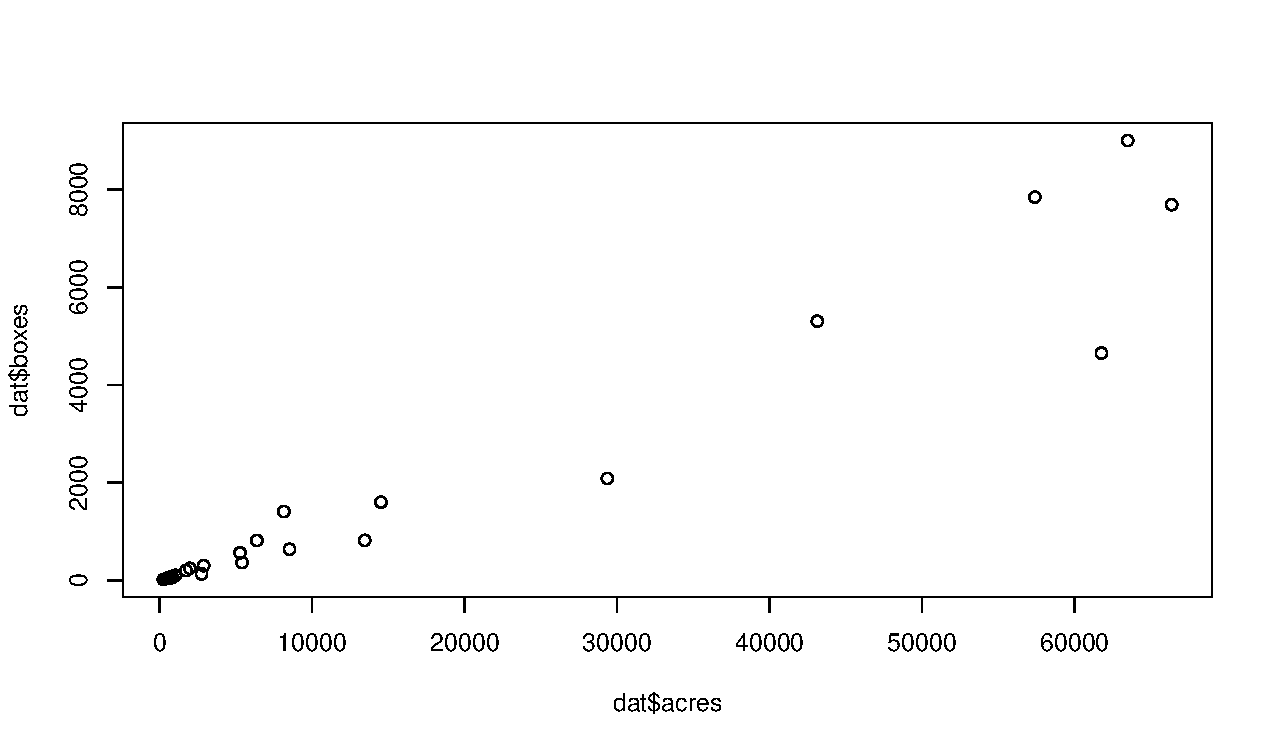
\includegraphics[width=\maxwidth]{figure/unnamed-chunk-54-1} 

}

\caption[Plot of Residuals by Fitted Values for Neuroblastoma Model with Age and Stage]{Plot of Residuals by Fitted Values for Neuroblastoma Model with Age and Stage}\label{fig:unnamed-chunk-54}
\end{figure}

\end{knitrout}
% \end{noindent}
Now we consider simplifying the model further by examining the decrease in the quality
of the fit that results from dropping the stage variable(s).
\[ \logit{\pi_i}=\beta_0+\beta_1x_{i1}+\beta_2x_{i2} \]
% \begin{noindent}
\begin{knitrout}
\definecolor{shadecolor}{rgb}{0.969, 0.969, 0.969}\color{fgcolor}\begin{kframe}
\begin{alltt}
\hlstd{model2} \hlkwb{=} \hlkwd{glm}\hlstd{(resp} \hlopt{~} \hlstd{agef,} \hlkwc{family} \hlstd{=} \hlkwd{binomial}\hlstd{(}\hlkwc{link} \hlstd{= logit),} \hlkwc{data} \hlstd{= neuro.dat)}
\hlkwd{summary}\hlstd{(model2)}
\end{alltt}
\begin{verbatim}

Call:
glm(formula = resp ~ agef, family = binomial(link = logit), data = neuro.dat)

Deviance Residuals: 
    Min       1Q   Median       3Q      Max  
-4.0853  -0.3591   1.5613   2.0684   3.4667  

Coefficients:
            Estimate Std. Error z value Pr(>|z|)    
(Intercept)   1.0415     0.2742   3.799 0.000145 ***
agef2        -2.1119     0.4325  -4.883 1.05e-06 ***
agef3        -3.0051     0.3827  -7.853 4.06e-15 ***
---
Signif. codes:  0 '***' 0.001 '**' 0.01 '*' 0.05 '.' 0.1 ' ' 1

(Dispersion parameter for binomial family taken to be 1)

    Null deviance: 162.832  on 14  degrees of freedom
Residual deviance:  83.583  on 12  degrees of freedom
AIC: 121.34

Number of Fisher Scoring iterations: 5
\end{verbatim}
\end{kframe}
\end{knitrout}
% \end{noindent}
Now we fit the model excluding the age variable to examine the drop in the quality of
fit from model one (with age and stage).
\[ \logit{\pi_i}=\beta_0+\beta_3x_{i3}+\beta_4x_{i4}+\beta_5x_{i5}+\beta_6x_{i6} \]
% \begin{noindent}
\begin{knitrout}
\definecolor{shadecolor}{rgb}{0.969, 0.969, 0.969}\color{fgcolor}\begin{kframe}
\begin{alltt}
\hlstd{model3} \hlkwb{=} \hlkwd{glm}\hlstd{(resp} \hlopt{~} \hlstd{stagef,} \hlkwc{family} \hlstd{=} \hlkwd{binomial}\hlstd{(}\hlkwc{link} \hlstd{= logit),}
  \hlkwc{data} \hlstd{= neuro.dat)}
\hlkwd{summary}\hlstd{(model3)}
\end{alltt}
\begin{verbatim}

Call:
glm(formula = resp ~ stagef, family = binomial(link = logit), 
    data = neuro.dat)

Deviance Residuals: 
    Min       1Q   Median       3Q      Max  
-2.0699  -1.5375  -0.5639   1.0444   2.9391  

Coefficients:
            Estimate Std. Error z value Pr(>|z|)    
(Intercept)   1.7918     0.6236   2.873  0.00406 ** 
stagef2      -1.2657     0.7150  -1.770  0.07671 .  
stagef3      -2.3224     0.7401  -3.138  0.00170 ** 
stagef4      -4.5643     0.7223  -6.319 2.63e-10 ***
stagef5      -0.5390     0.7766  -0.694  0.48768    
---
Signif. codes:  0 '***' 0.001 '**' 0.01 '*' 0.05 '.' 0.1 ' ' 1

(Dispersion parameter for binomial family taken to be 1)

    Null deviance: 162.832  on 14  degrees of freedom
Residual deviance:  42.446  on 10  degrees of freedom
AIC: 84.203

Number of Fisher Scoring iterations: 5
\end{verbatim}
\end{kframe}
\end{knitrout}
% \end{noindent}
\subsection*{Testing Nested Models}
Now we can consider testing nested models using \textcolor{Blue}{Deviance/Likelihood Ratio Tests}.
\begin{table}[!htbp]
      \centering
      \begin{NiceTabular}{cllcc}
            \toprule
            \textcolor{Blue}{Model} & \textcolor{Blue}{Factors In Model} & \textcolor{Blue}{Deviance} & $ \textcolor{Blue}{p} $ & $ \textcolor{Blue}{n-p} $\\
            \midrule
            1 & Age + Stage & $9.625$ & $ 7 $ & $ 8 $\\
            2 & Age & $83.583$ & $ 3 $ & $ 12 $\\
            3 & Stage & $42.446$ & $ 5 $ & $ 10 $\\
            4 & Intercept only & $162.832$ & $ 1 $ & $14 $\\
            \bottomrule
      \end{NiceTabular}
\end{table}
Recall:
\begin{align*}
      \Delta D
       & =D_0-D_\text{A}                                                                      \\
       & =-2\bigl(\ell(\hat{\Vector{\pi}})-\ell(\tilde{\Vector{\pi}})\bigr) \sim \chi^2_{q-p}
\end{align*}
where $ \hat{\Vector{\pi}} $ represents the MLEs from the \textcolor{Blue}{reduced (nested)} model and $ \tilde{\Vector{\pi}} $ are the MLEs from the \textcolor{Blue}{full} model.
\begin{Example}{}
      Task \#1: Pick the model that best represents the important associations between the
      outcome and explanatory variables.
\end{Example}
\begin{enumerate}[1.]
      \item \textcolor{Blue}{Is Stage important?}
            \begin{align*}
                  \HN & \colon \beta_3=\beta_4=\beta_5=\beta_6=0                                                      &  & \text{(Model 2 is adequate vs Model 1)} \\
                  \HA & \colon \beta_3\ne 0 \text{ or } \beta_4\ne 0 \text{ or } \beta_5\ne 0 \text{ or }\beta_6\ne 0 &  & \text{(Model 2 is not adequate)}
            \end{align*}
            \[ \Delta D=D_2-D_1=83.583-9.625=73.958 \]
            \[ p=\Prob{\chi^2_{7-3}>73.958}<0.001 \]
            % \begin{noindent}
\begin{knitrout}
\definecolor{shadecolor}{rgb}{0.969, 0.969, 0.969}\color{fgcolor}\begin{kframe}
\begin{alltt}
\hlnum{1} \hlopt{-} \hlkwd{pchisq}\hlstd{(model2}\hlopt{$}\hlstd{deviance} \hlopt{-} \hlstd{model1}\hlopt{$}\hlstd{deviance, model2}\hlopt{$}\hlstd{df.residual} \hlopt{-}
  \hlstd{model1}\hlopt{$}\hlstd{df.residual)}
\end{alltt}
\begin{verbatim}
[1] 3.330669e-15
\end{verbatim}
\end{kframe}
\end{knitrout}
          % \end{noindent}
            Therefore we reject the null hypothesis that stage is unimportant.
      \item \textcolor{Blue}{Is Age important?}
            \begin{align*}
                  \HN & \colon \beta_1=\beta_2=0                     &  & \text{(Model 3 is adequate vs Model 1)} \\
                  \HA & \colon \beta_1\ne 0 \text{ or } \beta_2\ne 0 &  & \text{(Model 3 is not adequate)}
            \end{align*}
            \[ \Delta D=D_3-D_1=42.446 - 9.625 = 32.821 \]
            \[ p=\Prob{\chi^2_{7-5}>32.821}<0.001 \]
            % \begin{noindent}
\begin{knitrout}
\definecolor{shadecolor}{rgb}{0.969, 0.969, 0.969}\color{fgcolor}\begin{kframe}
\begin{alltt}
\hlnum{1} \hlopt{-} \hlkwd{pchisq}\hlstd{(model3}\hlopt{$}\hlstd{deviance} \hlopt{-} \hlstd{model1}\hlopt{$}\hlstd{deviance, model3}\hlopt{$}\hlstd{df.residual} \hlopt{-}
  \hlstd{model1}\hlopt{$}\hlstd{df.residual)}
\end{alltt}
\begin{verbatim}
[1] 7.464321e-08
\end{verbatim}
\end{kframe}
\end{knitrout}
          % \end{noindent}
            Therefore we reject the null hypothesis that age is unimportant.
      \item \textcolor{Blue}{Do we need an Age$*$Stage interaction?}
            % \begin{noindent}
\begin{knitrout}
\definecolor{shadecolor}{rgb}{0.969, 0.969, 0.969}\color{fgcolor}\begin{kframe}
\begin{alltt}
\hlnum{1} \hlopt{-} \hlkwd{pchisq}\hlstd{(model1}\hlopt{$}\hlstd{deviance, model1}\hlopt{$}\hlstd{df.residual)}
\end{alltt}
\begin{verbatim}
[1] 0.292341
\end{verbatim}
\end{kframe}
\end{knitrout}
          % \end{noindent}
\end{enumerate}
So we select \textcolor{Blue}{Model 1} for interpretation. Here’s the fitted R \texttt{summary()} again for
reference.
\[ \logit{\pi_i}=\beta_0+\beta_1x_{i1}+\beta_2x_{i2}+\beta_3x_{i3}+\beta_4x_{i4}+\beta_5x_{i5}+\beta_6x_{i6} \]
% \begin{noindent}
\begin{knitrout}
\definecolor{shadecolor}{rgb}{0.969, 0.969, 0.969}\color{fgcolor}\begin{kframe}
\begin{alltt}
\hlstd{model1} \hlkwb{=} \hlkwd{glm}\hlstd{(resp} \hlopt{~} \hlstd{agef} \hlopt{+} \hlstd{stagef,} \hlkwc{family} \hlstd{=} \hlkwd{binomial}\hlstd{(}\hlkwc{link} \hlstd{= logit),}
  \hlkwc{data} \hlstd{= neuro.dat)}
\hlkwd{summary}\hlstd{(model1)}
\end{alltt}
\begin{verbatim}

Call:
glm(formula = resp ~ agef + stagef, family = binomial(link = logit), 
    data = neuro.dat)

Deviance Residuals: 
     Min        1Q    Median        3Q       Max  
-1.47408  -0.61913  -0.09643   0.53163   1.52114  

Coefficients:
            Estimate Std. Error z value Pr(>|z|)    
(Intercept)   3.3175     0.7721   4.297 1.73e-05 ***
agef2        -2.1181     0.5736  -3.693 0.000222 ***
agef3        -2.6130     0.5017  -5.208 1.91e-07 ***
stagef2      -1.2529     0.7837  -1.599 0.109860    
stagef3      -1.7759     0.8003  -2.219 0.026478 *  
stagef4      -4.3678     0.7902  -5.528 3.25e-08 ***
stagef5      -1.0222     0.8644  -1.183 0.236980    
---
Signif. codes:  0 '***' 0.001 '**' 0.01 '*' 0.05 '.' 0.1 ' ' 1

(Dispersion parameter for binomial family taken to be 1)

    Null deviance: 162.832  on 14  degrees of freedom
Residual deviance:   9.625  on  8  degrees of freedom
AIC: 55.382

Number of Fisher Scoring iterations: 4
\end{verbatim}
\end{kframe}
\end{knitrout}
% \end{noindent}
\subsection*{Model Interpretation}
\begin{Example}{}
      Task \#2: Interpret the selected model through estimated ORs.
\end{Example}
\begin{enumerate}[A.]
      \item \textcolor{Blue}{What is the odds ratio of surviving two years for a patient with disease in stage IV versus stage I?}
            \begin{table}[!htbp]
                  \centering
                  \begin{NiceTabular}{cccc}
                        Age & Stage & $ (1,x_{i1},x_{i2},x_{i3},x_{i4},x_{i5},x_{i6})^\top $ & $ \log[\big]{\pi_i/(1-\pi_i)} $\\
                        \midrule
                        NA & IV & $ (1,x_{i1},x_{i2},0,0,1,0)^\top $ & $ \beta_0+\beta_1x_{i1}+\beta_2x_{i2}+\beta_5 $\\
                        NA & I & $ (1,x_{i1},x_{i2},0,0,0,0)^\top $ & $ \beta_0+\beta_1x_{i1}+\beta_2x_{i2} $\\
                        \bottomrule
                  \end{NiceTabular}
            \end{table}
            \[ \widehat{\text{OR}}=\exp{\hat{\beta}_5}=\exp{-4.368}=0.013 \]
            When controlling for age, the odds of surviving two years among those diagnosed
            in state IV is $0.013$ times the odds among subjects diagnosed in stage I.
      \item \textcolor{Blue}{What is the odds ratio of surviving for a patient aged 24+ months versus 12-23 months?}
            \begin{table}[!htbp]
                  \centering
                  \begin{NiceTabular}{cccc}
                        Age & Stage & $ (1,x_{i1},x_{i2},x_{i3},x_{i4},x_{i5},x_{i6})^\top $ & $ \log[\big]{\pi_i/(1-\pi_i)} $\\
                        \midrule
                        24+ & NA & $ (1,0,1,x_{i3},x_{i4},x_{i5},x_{i6})^\top $ & $ \beta_0+\beta_2+\beta_3x_{i3}+\beta_4x_{i4}+\beta_5x_{i5}+\beta_6x_{i6} $\\
                        12-23 & NA & $ (1,1,0,x_{i3},x_{i4},x_{i5},x_{i6})^\top $ & $ \beta_0+\beta_1+\beta_3x_{i3}+\beta_4x_{i4}+\beta_5x_{i5}+\beta_6x_{i6}$\\
                        \bottomrule
                  \end{NiceTabular}
            \end{table}
            \[ \widehat{\text{OR}}=\exp{\hat{\beta}_2-\hat{\beta}_1}=\exp[\big]{-2.613-(-2.118)}=0.61 \]
            When controlling for stage, the odds of surviving two years among those diagnosed at
            24+ months of age is $0.61$ times the odds of surviving two years among subjects
            diagnosed at 12-23 months of age.
\end{enumerate}
\subsection*{Constructing Confidence Intervals}
\begin{Example}{}
      Task \#3: Get Confidence Intervals for our estimated ORs.
\end{Example}
\begin{enumerate}[A.]
      \item $ \text{OR}=\exp{\beta_5} $, so we can use a Wald-based CI,
            \[ \exp[\big]{\hat{\beta}_5\pm 1.96\se{\hat{\beta}_5}}=\exp[\big]{-4.368\pm 1.96(0.7902)}=(0.003,0.060) \]
      \item What about a CI for $ \text{OR}=\exp{\beta_2-\beta_1} $?
            \begin{itemize}
                  \item In order to calculate a CI we need to obtain $ \se{\hat{\beta}_2-\hat{\beta}_1} $.
                  \item This is not directly available from R \texttt{summary()}.
                        \begin{align*}
                              \Var{aX+bY}                       & =a^2\Var{X}+b^2\Var{Y}+2ab\Cov{X,Y}                                         \\
                              \Var{\hat{\beta}_2-\hat{\beta}_1} & =\Var{\hat{\beta}_2}+\Var{\hat{\beta}_1}-2\Cov{\hat{\beta}_2,\hat{\beta}_1}
                        \end{align*}
                  \item The covariance matrix ($ \Matrix{I}^{-1} $) is available from \texttt{summary(model1)\$cov.unscaled}.
            \end{itemize}
\end{enumerate}
\subsection*{2.9 Confidence Intervals for non-linear functions of $ \eta_i $}
\addcontentsline{toc}{subsection}{Confidence Intervals for non-linear functions of \texorpdfstring{$ \eta_i $}{ηi}}
Recall that since $ \hat{\Vector{\beta}} $ is an MLE, $ \textcolor{Blue}{\hat{\Vector{\beta}} \sim \MVN[\big]{\beta,\Matrix{I}^{-1}(\hat{\Vector{\beta}})}} $ approximately. This means that:
\[ \Vector{x}_i^\top \hat{\Vector{\beta}}\sim \N[\big]{\Vector{x}_i^\top \Vector{\beta},\Vector{x}_i^\top \Matrix{I}^{-1}(\hat{\Vector{\beta}})\Vector{x}_i} \]
and
\[ \frac{\Vector{x}_i^\top \hat{\Vector{\beta}}-\Vector{x}_i^\top \Vector{\beta}}{\sqrt{\Vector{x}_i^\top \Matrix{I}^{-1}(\hat{\Vector{\beta}})\Vector{x}_i}} \sim \N{0,1}  \]
\begin{Regular}{}
      \begin{enumerate}[1.]
            \item An approximate \qty{95}{\percent} CI for $ \eta_i=\Vector{x}_i^\top \Vector{\beta} $ is then given by:
                  \[ \Vector{x}_i^\top \hat{\Vector{\beta}}\pm 1.96\sqrt{\Vector{x}_i^\top \Matrix{I}^{-1}(\hat{\Vector{\beta}})\Vector{x}_i}=(\hat{\eta}_\text{L},\hat{\eta}_\text{U}) \]
            \item If the OR of interest is expressed as $ \exp{\Vector{c}^\top \Vector{\beta}} $ where $ \Vector{c} $ is a column vector defining
                  the contrast of the regression coefficients, then an approximate \qty{95}{\percent} CI for this OR is:
                  \[ \exp*{\Vector{c}^\top\hat{\Vector{\beta}}\pm 1.96\sqrt{\Vector{c}^\top\Matrix{I}^{-1}(\hat{\Vector{\beta}})\Vector{c}}} \]
            \item An approximate \qty{95}{\percent} CI for $ \pi_i=\exp{\Vector{x}_i^\top \Vector{\beta}}/\bigl(1+\exp{\Vector{x}_i^\top \Vector{\beta}}\bigr)=\expit{\Vector{x}_i^\top \Vector{\beta}}. $ is:
                  \[ \Bigl(\expit{\hat{\eta}_\text{L}},\expit{\hat{\eta}_\text{U}}\Bigr). \]
      \end{enumerate}
\end{Regular}
\subsection*{Back to the Neuroblastoma Example}
\begin{enumerate}[B.]
      \item Find a confidence interval for $ \text{OR}=\exp{\beta_2-\beta_1} $.
            \begin{itemize}
                  \item The vector defining the contrast of interest is $ \Vector{c}=(0,-1,1,0,0,0,0)^\top $:
                        \[ \Vector{c}^\top \hat{\Vector{\beta}}=\begin{bmatrix}
                                    0 & -1 & 1 & 0 & 0 & 0 & 0
                              \end{bmatrix}\begin{bmatrix}
                                    \hat{\beta}_0 \\
                                    \hat{\beta}_1 \\
                                    \vdots        \\
                                    \hat{\beta}_6
                              \end{bmatrix}=\hat{\beta}_2-\hat{\beta}_1 \]
                        \begin{align*}
                              \Vector{c}^\top \Matrix{I}^{-1}(\hat{\Vector{\beta}})\Vector{c} & =\begin{bmatrix}
                                                                                                       0 & -1 & 1 & 0 & 0 & 0 & 0
                                                                                                 \end{bmatrix}\begin{bmatrix}
                                                                                                                    I^{00}     & I^{01}     & I^{02}     & \cdots & I^{0(p-1)}     \\
                                                                                                                    I^{10}     & I^{11}     & I^{12}     & \cdots & I^{1(p-1)}     \\
                                                                                                                    I^{21}     & I^{21}     & I^{22}     & \cdots & I^{2(p-1)}     \\
                                                                                                                    \vdots     & \vdots     & \vdots     & \ddots & \vdots         \\
                                                                                                                    I^{(p-1)1} & I^{(p-1)1} & I^{(p-1)2} & \cdots & I^{(p-1)(p-1)}
                                                                                                              \end{bmatrix}\begin{bmatrix}
                                                                                                                                 0  \\
                                                                                                                                 -1 \\
                                                                                                                                 1  \\
                                                                                                                                 0  \\
                                                                                                                                 0  \\
                                                                                                                                 0  \\
                                                                                                                                 0
                                                                                                                           \end{bmatrix} \\
                                                                                              & =I^{11} + I^{22} - I^{12} - I^{21}                                           \\
                                                                                              & =\Var{\hat{\beta}_2}+\Var{\hat{\beta}_1}-2\Cov{\hat{\beta}_2,\hat{\beta}_1}
                        \end{align*}
                  \item The program used to compute the variance is as follows:
                        % \begin{noindent}
\begin{knitrout}
\definecolor{shadecolor}{rgb}{0.969, 0.969, 0.969}\color{fgcolor}\begin{kframe}
\begin{alltt}
\hlcom{# use the summary.glm function and store the result in the}
\hlcom{# tmp object}
\hlstd{tmp} \hlkwb{=} \hlkwd{summary.glm}\hlstd{(model1)}
\hlcom{# examine the contents of the tmp objects and store the}
\hlcom{# covariance matrix in v}
\hlkwd{names}\hlstd{(tmp)}
\hlstd{v} \hlkwb{=} \hlstd{tmp}\hlopt{$}\hlstd{cov.unscaled}
\hlstd{v}
\hlcom{# create x vector to get contrast of regression}
\hlcom{# coefficients}
\hlstd{x} \hlkwb{=} \hlkwd{c}\hlstd{(}\hlnum{0}\hlstd{,} \hlopt{-}\hlnum{1}\hlstd{,} \hlnum{1}\hlstd{,} \hlnum{0}\hlstd{,} \hlnum{0}\hlstd{,} \hlnum{0}\hlstd{,} \hlnum{0}\hlstd{)}
\hlstd{x} \hlkwb{=} \hlkwd{as.matrix}\hlstd{(x,} \hlnum{7}\hlstd{,} \hlnum{1}\hlstd{)}
\hlkwd{dim}\hlstd{(x)}
\hlcom{# compute the variance estimate of difference in estimates}
\hlcom{# for age parameters}
\hlkwd{t}\hlstd{(x)} \hlopt \hlstd{v} \hlopt \hlstd{x}
\end{alltt}
\end{kframe}
\end{knitrout}
                % \end{noindent}
                  \item The resulting output is as follows.
\begin{knitrout}
\definecolor{shadecolor}{rgb}{0.969, 0.969, 0.969}\color{fgcolor}\begin{kframe}
\begin{alltt}
\hlcom{# use the summary.glm function and store the result in the}
\hlcom{# tmp object}
\hlstd{tmp} \hlkwb{=} \hlkwd{summary.glm}\hlstd{(model1)}
\hlcom{# examine the contents of the tmp objects and store the}
\hlcom{# covariance matrix in v}
\hlkwd{names}\hlstd{(tmp)}
\end{alltt}
\begin{verbatim}
 [1] "call"           "terms"          "family"         "deviance"      
 [5] "aic"            "contrasts"      "df.residual"    "null.deviance" 
 [9] "df.null"        "iter"           "deviance.resid" "coefficients"  
[13] "aliased"        "dispersion"     "df"             "cov.unscaled"  
[17] "cov.scaled"    
\end{verbatim}
\begin{alltt}
\hlstd{v} \hlkwb{=} \hlstd{tmp}\hlopt{$}\hlstd{cov.unscaled}
\hlstd{v}
\end{alltt}
\begin{verbatim}
            (Intercept)       agef2       agef3     stagef2     stagef3
(Intercept)   0.5960933 -0.18392302 -0.17583962 -0.46378468 -0.43679598
agef2        -0.1839230  0.32901185  0.15792411  0.01837858 -0.01638010
agef3        -0.1758396  0.15792411  0.25170695  0.01648743 -0.01538075
stagef2      -0.4637847  0.01837858  0.01648743  0.61411717  0.44845241
stagef3      -0.4367960 -0.01638010 -0.01538075  0.44845241  0.64043301
stagef4      -0.5098913  0.08279176  0.06769368  0.45553801  0.44437841
stagef5      -0.4969598  0.06047881  0.05606300  0.45425149  0.44552862
                stagef4     stagef5
(Intercept) -0.50989130 -0.49695978
agef2        0.08279176  0.06047881
agef3        0.06769368  0.05606300
stagef2      0.45553801  0.45425149
stagef3      0.44437841  0.44552862
stagef4      0.62439906  0.46920985
stagef5      0.46920985  0.74722885
\end{verbatim}
\begin{alltt}
\hlstd{x} \hlkwb{=} \hlkwd{c}\hlstd{(}\hlnum{0}\hlstd{,} \hlopt{-}\hlnum{1}\hlstd{,} \hlnum{1}\hlstd{,} \hlnum{0}\hlstd{,} \hlnum{0}\hlstd{,} \hlnum{0}\hlstd{,} \hlnum{0}\hlstd{)}
\hlstd{x} \hlkwb{=} \hlkwd{as.matrix}\hlstd{(x,} \hlnum{7}\hlstd{,} \hlnum{1}\hlstd{)}
\hlkwd{dim}\hlstd{(x)}
\end{alltt}
\begin{verbatim}
[1] 7 1
\end{verbatim}
\begin{alltt}
\hlcom{# compute the variance estimate of difference in estimates}
\hlcom{# for age parameters}
\hlkwd{t}\hlstd{(x)} \hlopt \hlstd{v} \hlopt \hlstd{x}
\end{alltt}
\begin{verbatim}
          [,1]
[1,] 0.2648706
\end{verbatim}
\end{kframe}
\end{knitrout}
                        % \end{noindent}
                  \item We previously found that:
                        \[ \widehat{\text{OR}}=\exp{\hat{\beta}_2-\hat{\beta}_1}=\exp[\big]{-2.613-(-2.118)}=0.61 \]
                  \item From the new R output, we have calculated:
                        \[ \estVar{\hat{\beta}_2-\hat{\beta}_1}=0.2649 \]
                  \item An approximate \qty{95}{\percent} CI for $ \beta_2-\beta_1 $ is therefore:
                        \[ -0.495\pm 1.96\sqrt{0.2649}=(-1.504,0.514) \]
                  \item The corresponding interval for the odds ratio is:
                        \[ \exp[\big]{(-1.504,0.514)}=(0.22,1.67) \]
            \end{itemize}
\end{enumerate}

\section*{Topic 2e: Bioassay and Dose Response Models}
\addcontentsline{toc}{section}{Topic 2e: Bioassay and Dose Response Models}
\begin{itemize}
    \item \textcolor{Blue}{Previously}: Logistic regression analysis of Binomial data with binary and
          categorical explanatory variables.
    \item \textcolor{Blue}{Today}: Explore different link functions and continuous explanatory variables.
\end{itemize}
\begin{enumerate}[1.]
    \item Modelling the Dose Response Relationship.
          \begin{itemize}
              \item Tolerance distributions and their associated links.
              \item Finding the median lethal/effective dose.
          \end{itemize}
    \item Beetle Mortality Example.
\end{enumerate}
\subsection*{2.10 Bioassay and Dose Response Models}
\addcontentsline{toc}{subsection}{Modelling the Dose Response Relationship}
\begin{itemize}
    \item \textcolor{Blue}{Bioassay experiment}: Expose several groups of subjects to varying levels of a
          toxin/drug and determine how many responses within a fixed period of time.
    \item \textcolor{Blue}{Stimulus}: Each group is subjected to a particular dose of the toxin/drug:
          \[ \textcolor{Green}{\text{dose}=\log{\text{concentration}}} \]
    \item \textcolor{Blue}{Response}: As a result of the stimulus, subjects will manifest a binary response
          (often of the form died/survived).
    \item \textcolor{Blue}{Tolerance}: We assume that for each subject there is a certain dose level above
          which the response will always occur.
          \begin{itemize}
              \item This level is called the tolerance or threshold.
              \item The tolerance varies from one individual to another in the population and therefore
                    from subject to subject in the sample.
              \item We can therefore ascribe a distribution to it.
          \end{itemize}
\end{itemize}
\subsection*{The Tolerance Distribution}
\begin{itemize}
    \item $ z =$ concentration of the stimulus (toxin/drug).
    \item $ x=\log{z} =$ dose/intensity of the stimulus.
    \item $ f(x)= $ pdf for the distribution of the tolerance in the population (\emph{i.e., the
              distribution for the stimulus/dose at which response occurs}).
    \item Suppose a dose of $ x_0 $ were applied to the population. What proportion would
          respond?
          \[ \pi_0=\int_{-\infty}^{x_0}f(s)\odif{s} \]
    \item If $ x_0<x_1 $, then $ \pi_0<\pi_1 $.
\end{itemize}
\subsection*{Modelling the Dose Response Relationship}
For each group $ j=1,\ldots,J $ let:
\begin{itemize}
    \item $ m_j= $ number of subjects in group $ j $.
    \item $ x_j= $ dose applied to subjects in group $ j $.
    \item $ y_j= $ the number of subjects with response in group $ j $.
\end{itemize}
\begin{table}[!htbp]
    \centering
    \begin{NiceTabular}{cccc}
        \toprule
        Dose & Responders & Total\\
        $ x_j $ & $ y_j $ & $ m_j $ & $ y_j/m_j $\\
        \midrule
        $ 1.6907 $ & $ 6 $ & $ 59 $ & $ 0.10 $\\
        $ 1.7242 $ & $ 13 $ & $ 60 $ & $ 0.22 $\\
        $ 1.7552 $ & $ 18 $ & $ 62 $ & $ 0.29 $\\
        \bottomrule
    \end{NiceTabular}
\end{table}
Assume
\[ \textcolor{Blue}{Y_j \sim \BIN{m_j,\pi_j},\qquad j=1,\ldots,J} \text{ independently} \]
where $ \pi_j= $ probability of response in group $ j $ (i.e., at dose $ x_j $).
\begin{itemize}
    \item \textcolor{Blue}{Goal}: To model $ \pi_j=\pi_j(x_j) $ as a function of the continuous stimulus/dose covariate $ x_j $.
    \item Since $ 0\le \pi\le 1 $, the usual setup is to model using:
          \[ g(\pi)=\beta_0+\beta_1x=\eta \]
          where $ g(\:\cdot\:) $ is a link function.
    \item Then we have:
          \[ \pi(x)=g^{-1}(\beta_0+\beta_1x) \]
    \item What link function should we select?
\end{itemize}
\subsection*{Typical Dose Response Curve}
TODO figure
\begin{itemize}
    \item This suggests selecting $ g(\:\cdot\:) $ such that $ g^{-1}(\:\cdot\:) $ is a cdf:
          \[ \pi(x)=g^{-1}(\beta_0+\beta_1x)=F^*(\beta_0+\beta_1x) \]
\end{itemize}
\subsection*{The Link Function and the Tolerance Distribution}
\begin{itemize}
    \item Now we have an inverse link function that is a cdf:
          \[ \pi(x)=g^{-1}(\beta_0+\beta_1x)=F^*(\beta_0+\beta_1x) \]
    \item Recall our original definition of the \textcolor{Blue}{tolerance distribution}:
          \[ \pi(x)=\int_{-\infty}^{x}f(s)\odif{s} \]
    \item So if we select a tolerance distribution that will determine the link function
          through:
          \[ \textcolor{Blue}{\pi(x)=g^{-1}(\beta_0+\beta_1x)=F^*(\beta_0+\beta_1x)=\int_{-\infty}^{\infty}f(s)\odif{s}} \]
    \item $ f(x) $ determines how the ``probability of a positive response'' changes with the value of the dose.
          \[ \pdv{\pi(x)}{x}=(F^*)^\prime (\beta_0+\beta_1x)(\beta_1)=f(x) \]
\end{itemize}
\subsection*{Some Choices for the Tolerance Distribution}
\begin{enumerate}[1.]
    \item \textcolor{Red}{Normal Tolerance Distribution} ($ f(s) $ is Normal pdf):
          \begin{align*}
              \pi(x)
               & =\int_{-\infty}^{x}f(s)\odif{s}                                                                                        \\
               & =\int_{-\infty}^{x}\frac{1}{\sqrt{2\pi\sigma^2}} \exp*{-\frac{1}{2} \biggl(\frac{s-\mu}{\sigma} \biggr)^{\!2}}\odif{s} \\
               & =\Phi\biggl(\frac{x-\mu}{\sigma}\biggr)
          \end{align*}
          where $ \Phi $ is the $ \N{0,1} $ cdf. This implies:
          \begin{align*}
              g^{-1}(\beta_0+\beta_1x)    & =\Phi\biggl(\frac{x-\mu}{\sigma}\biggr)                          \\
              \pi(x)                      & =g^{-1}(\beta_0+\beta_1x)=\Phi\biggl(\frac{x-\mu}{\sigma}\biggr) \\
              \Phi^{-1}\bigl(\pi(x)\bigr) & =\beta_0+\beta_1x=\frac{x-\mu}{\sigma}
          \end{align*}
          We call this the \textcolor{Blue}{Probit link} $ g(\:\cdot\:)=\Phi^{-1}(\:\cdot\:) $.
\end{enumerate}
\begin{enumerate}[1.]
    \item How do we interpret $ \beta_0 $ and $ \beta_1 $?
          \begin{itemize}
              \item They are no longer log odds ratios (as with logistic link).
              \item Interpretation is in terms of $ \mu $ and $ \sigma $ the parameters of the tolerance distribution.
          \end{itemize}
          \[ \pi(x)=g^{-1}(\beta_0+\beta_1x)=\Phi\biggl(\frac{x-\mu}{\sigma} \biggr)=\Phi\biggl(\frac{x}{\sigma} -\frac{\mu}{\sigma} \biggr) \]
          \[ \beta_0=\frac{-\mu}{\sigma},\qquad \beta_1=\frac{1}{\sigma} \]
\end{enumerate}
\subsection*{Median lethal/effective dose}
Let $ \delta $ be the \textcolor{Blue}{median lethal/effective dose}.
\begin{itemize}
    \item The dose $ \delta $ at which \qty{50}{\percent} of the population has the response i.e., $ \pi(\delta)=0.50 $.
    \item Find an expression for $ \delta $ in terms of $ \beta_0 $ and $ \beta_1 $:
          \begin{align*}
              \Phi^{-1}\bigl(\pi(x)\bigr) & =\beta_0+\beta_1x         \\
              \Phi^{-1}(0.50)             & =\beta_0+\beta_1\delta    \\
              0                           & =\beta_0+\beta_1\delta    \\
              \delta                      & =\frac{-\beta_0}{\beta_1}
          \end{align*}
    \item Can also find other quantiles of the tolerance distribution i.e., $ \pi(\delta_p)=p $, $ 0<p<1 $.
\end{itemize}
\begin{table}[!htbp]
    \centering
    \begin{NiceTabular}{ccc}
        \toprule
        \multicolumn{2}{c}{\textcolor{Blue}{Tolerance Distribution}} & \textcolor{Blue}{Link Function}\\
        Name & $ \pi=g^{-1}(\eta) $ & $ \eta=g(\pi) $\\
        \midrule
        \textcolor{Red}{Normal} & $\begin{aligned}
                \pi(x) & =\int_{-\infty}^{x}\frac{\beta_1}{\sqrt{2\pi}}\exp*{-\frac{1}{2}(\beta_0+\beta_1s)^2} \odif{s} \\
                       & =\Phi(\beta_0+\beta_1x)                                                                        \\
                       & =\Phi(\eta)
            \end{aligned}$ & $\begin{array}{c}
                \eta=\Phi^{-1}(\pi) \\
                \textcolor{Red}{\text{probit}}
            \end{array}$\\
        \midrule
        \textcolor{Red}{Logistic} & $\begin{aligned}
                \pi(x) & =\int_{-\infty}^{x}\frac{\beta_1\exp{\beta_0+\beta_1s}}{(1+\exp{\beta_0+\beta_1s})^2} \odif{s} \\
                       & =\frac{\exp*{\beta_0+\beta_1x}}{1+\exp{\beta_0+\beta_1x}}                                      \\
                       & =\frac{\exp{\eta}}{1+\exp{\eta}}
            \end{aligned}$ & $\begin{array}{c}
                \eta=\log*{\frac{\pi}{1-\pi}} \\
                \textcolor{Red}{\text{logistic}}
            \end{array}$\\
        \midrule
        \textcolor{Red}{Extreme Value} & $\begin{aligned}
                \pi(x) & =\int_{-\infty}^{x}\beta_1\exp[\big]{\beta_0+\beta_1s-\exp{\beta_0+\beta_1s}} \odif{s} \\
                       & =\int_{-\infty}^{\eta}\exp[\big]{\nu-\exp{\nu}}\odif{\nu}                              \\
                       & =1-\exp[\big]{-\exp{\eta}}
            \end{aligned}$ & $\begin{array}{c}
                \eta=\log[\big]{-\log{1-\pi}} \\
                \textcolor{Red}{\text{complementary log-log}}
            \end{array}$\\
        \bottomrule
    \end{NiceTabular}
\end{table}
\subsection*{A Dose Response Example}
\addcontentsline{toc}{subsection}{A Dose Response Example}
\begin{Example}{Beetle Mortality}
    Consider an experiment by Bliss (Annals of Applied Biology, 1935) in which groups of
    beetles were exposed to varying concentrations of carbon disulphide ($\text{CS}_2$) gas.
    \begin{center}
        \begin{NiceTabular}{cccc}
            \toprule
            &\text{\# of insects} & \text{\# of insects}\\
            Dose ($ x_i $) & killed ($ x_i $) & $ m_i $ & $ y_j/m_i $\\
            \midrule
            $ 1.6907 $ & $ 6 $ & $ 59 $ & $ 0.10 $\\
            $ 1.7242 $ & $ 13 $ & $ 60 $ & $ 0.22 $\\
            $ 1.7552 $ & $ 18 $ & $ 62 $ & $ 0.29 $\\
            $1.7842$ & $28$ & $56$ & $0.50$\\
            $1.8113$ & $52$ & $63$ & $0.83$\\
            $1.8369$ & $53$ & $59$ & $0.89$\\
            $1.8610$ & $61$ & $62$ & $0.98$\\
            $1.8839$ & $60$ & $60$ & $1.00$\\
            \bottomrule
        \end{NiceTabular}
    \end{center}
\end{Example}
\subsection*{R Data and Code}
\begin{Example}{Data file \texttt{beetle.dat}}
    % \begin{noindent}
\begin{knitrout}
\definecolor{shadecolor}{rgb}{0.969, 0.969, 0.969}\color{fgcolor}\begin{kframe}
\begin{verbatim}
    dose  y  m
1 1.6907  6 59
2 1.7242 13 60
3 1.7552 18 62
4 1.7842 28 56
5 1.8113 52 63
6 1.8369 53 59
7 1.8610 61 62
8 1.8839 60 60
\end{verbatim}
\end{kframe}
\end{knitrout}
      % \end{noindent}
\end{Example}
\begin{itemize}
    \item Recall we are interested in modelling the \textcolor{Blue}{dose-response relationship}:
          \[ \pi(x)=g^{-1}(\beta_0+\beta_1x) \]
          where $ x= $ dose.
    \item We will fit several binomial regression
          models to this data.
    \item Use various link functions to find the best
          model.
\end{itemize}
% \begin{noindent}
\begin{knitrout}
\definecolor{shadecolor}{rgb}{0.969, 0.969, 0.969}\color{fgcolor}\begin{kframe}
\begin{alltt}
\hlcom{# R program for analysis of dose-response data}
\hlstd{beetle.dat} \hlkwb{=} \hlkwd{read.table}\hlstd{(}\hlstr{"beetle.dat"}\hlstd{,} \hlkwc{header} \hlstd{= T)}
\hlcom{# here we construct the response variable for logistic}
\hlcom{# regression}
\hlstd{beetle.dat}\hlopt{$}\hlstd{resp} \hlkwb{=} \hlkwd{cbind}\hlstd{(beetle.dat}\hlopt{$}\hlstd{y, beetle.dat}\hlopt{$}\hlstd{m} \hlopt{-} \hlstd{beetle.dat}\hlopt{$}\hlstd{y)}
\hlstd{beetle.dat}
\hlcom{# here we fit a logistic model involving dose}
\hlstd{model1} \hlkwb{=} \hlkwd{glm}\hlstd{(resp} \hlopt{~} \hlstd{dose,} \hlkwc{family} \hlstd{=} \hlkwd{binomial}\hlstd{(}\hlkwc{link} \hlstd{= logit),} \hlkwc{data} \hlstd{= beetle.dat)}
\hlkwd{summary}\hlstd{(model1)}
\hlcom{# here we record deviance residuals in rd1}
\hlstd{rd1} \hlkwb{=} \hlkwd{residuals.glm}\hlstd{(model1,} \hlstr{"deviance"}\hlstd{)}
\hlstd{fv1} \hlkwb{=} \hlstd{model1}\hlopt{$}\hlstd{fitted.values}
\hlcom{# plotting the deviance residuals by dose and by fitted}
\hlcom{# values}
\hlkwd{pdf}\hlstd{(}\hlstr{"beetle-residuals.pdf"}\hlstd{,} \hlkwc{width} \hlstd{=} \hlnum{10}\hlstd{,} \hlkwc{height} \hlstd{=} \hlnum{8}\hlstd{)}
\hlkwd{par}\hlstd{(}\hlkwc{mfrow} \hlstd{=} \hlkwd{c}\hlstd{(}\hlnum{3}\hlstd{,} \hlnum{2}\hlstd{))}
\hlkwd{plot}\hlstd{(beetle.dat}\hlopt{$}\hlstd{dose, rd1,} \hlkwc{ylim} \hlstd{=} \hlkwd{c}\hlstd{(}\hlopt{-}\hlnum{5}\hlstd{,} \hlnum{5}\hlstd{),} \hlkwc{xlab} \hlstd{=} \hlstr{"DOSE"}\hlstd{,} \hlkwc{ylab} \hlstd{=} \hlstr{"DEVIANCE RESIDUALS"}\hlstd{)}
\hlkwd{abline}\hlstd{(}\hlkwc{h} \hlstd{=} \hlopt{-}\hlnum{2}\hlstd{)}
\hlkwd{abline}\hlstd{(}\hlkwc{h} \hlstd{=} \hlnum{2}\hlstd{)}
\hlkwd{title}\hlstd{(}\hlstr{"Model 1 - logit link"}\hlstd{)}
\hlkwd{plot}\hlstd{(fv1, rd1,} \hlkwc{ylim} \hlstd{=} \hlkwd{c}\hlstd{(}\hlopt{-}\hlnum{5}\hlstd{,} \hlnum{5}\hlstd{),} \hlkwc{xlab} \hlstd{=} \hlstr{"FITTED VALUE"}\hlstd{,} \hlkwc{ylab} \hlstd{=} \hlstr{"DEVIANCE RESIDUALS"}\hlstd{)}
\hlkwd{abline}\hlstd{(}\hlkwc{h} \hlstd{=} \hlopt{-}\hlnum{2}\hlstd{)}
\hlkwd{abline}\hlstd{(}\hlkwc{h} \hlstd{=} \hlnum{2}\hlstd{)}
\hlkwd{title}\hlstd{(}\hlstr{"Model 1 - logit link"}\hlstd{)}
\hlcom{# here we fit a probit model involving dose}
\hlstd{model2} \hlkwb{=} \hlkwd{glm}\hlstd{(resp} \hlopt{~} \hlstd{dose,} \hlkwc{family} \hlstd{=} \hlkwd{binomial}\hlstd{(}\hlkwc{link} \hlstd{= probit),} \hlkwc{data} \hlstd{= beetle.dat)}
\hlkwd{summary}\hlstd{(model2)}
\hlstd{rd2} \hlkwb{=} \hlkwd{residuals.glm}\hlstd{(model2,} \hlstr{"deviance"}\hlstd{)}
\hlstd{fv2} \hlkwb{=} \hlstd{model2}\hlopt{$}\hlstd{fitted.values}
\hlcom{# here we fit a complementary log-log model involving dose}
\hlstd{model3} \hlkwb{=} \hlkwd{glm}\hlstd{(resp} \hlopt{~} \hlstd{dose,} \hlkwc{family} \hlstd{=} \hlkwd{binomial}\hlstd{(}\hlkwc{link} \hlstd{= cloglog),}
  \hlkwc{data} \hlstd{= beetle.dat)}
\hlkwd{summary}\hlstd{(model3)}
\hlstd{rd3} \hlkwb{=} \hlkwd{residuals.glm}\hlstd{(model3,} \hlstr{"deviance"}\hlstd{)}
\hlstd{fv3} \hlkwb{=} \hlstd{model3}\hlopt{$}\hlstd{fitted.values}
\hlkwd{plot}\hlstd{(beetle.dat}\hlopt{$}\hlstd{dose, rd2,} \hlkwc{ylim} \hlstd{=} \hlkwd{c}\hlstd{(}\hlopt{-}\hlnum{5}\hlstd{,} \hlnum{5}\hlstd{),} \hlkwc{xlab} \hlstd{=} \hlstr{"DOSE"}\hlstd{,} \hlkwc{ylab} \hlstd{=} \hlstr{"DEVIANCE RESIDUALS"}\hlstd{)}
\hlkwd{abline}\hlstd{(}\hlkwc{h} \hlstd{=} \hlopt{-}\hlnum{2}\hlstd{)}
\hlkwd{abline}\hlstd{(}\hlkwc{h} \hlstd{=} \hlnum{2}\hlstd{)}
\hlkwd{title}\hlstd{(}\hlstr{"Model 2 - probit link"}\hlstd{)}
\hlkwd{plot}\hlstd{(fv2, rd2,} \hlkwc{ylim} \hlstd{=} \hlkwd{c}\hlstd{(}\hlopt{-}\hlnum{5}\hlstd{,} \hlnum{5}\hlstd{),} \hlkwc{xlab} \hlstd{=} \hlstr{"FITTED VALUE"}\hlstd{,} \hlkwc{ylab} \hlstd{=} \hlstr{"DEVIANCE RESIDUALS"}\hlstd{)}
\hlkwd{abline}\hlstd{(}\hlkwc{h} \hlstd{=} \hlopt{-}\hlnum{2}\hlstd{)}
\hlkwd{abline}\hlstd{(}\hlkwc{h} \hlstd{=} \hlnum{2}\hlstd{)}
\hlkwd{title}\hlstd{(}\hlstr{"Model 2 - probit link"}\hlstd{)}
\hlkwd{plot}\hlstd{(beetle.dat}\hlopt{$}\hlstd{dose, rd3,} \hlkwc{ylim} \hlstd{=} \hlkwd{c}\hlstd{(}\hlopt{-}\hlnum{5}\hlstd{,} \hlnum{5}\hlstd{),} \hlkwc{xlab} \hlstd{=} \hlstr{"DOSE"}\hlstd{,} \hlkwc{ylab} \hlstd{=} \hlstr{"DEVIANCE RESIDUALS"}\hlstd{)}
\hlkwd{abline}\hlstd{(}\hlkwc{h} \hlstd{=} \hlopt{-}\hlnum{2}\hlstd{)}
\hlkwd{abline}\hlstd{(}\hlkwc{h} \hlstd{=} \hlnum{2}\hlstd{)}
\hlkwd{title}\hlstd{(}\hlstr{"Model 3 - log-log link"}\hlstd{)}
\hlkwd{plot}\hlstd{(fv3, rd3,} \hlkwc{ylim} \hlstd{=} \hlkwd{c}\hlstd{(}\hlopt{-}\hlnum{5}\hlstd{,} \hlnum{5}\hlstd{),} \hlkwc{xlab} \hlstd{=} \hlstr{"FITTED VALUE"}\hlstd{,} \hlkwc{ylab} \hlstd{=} \hlstr{"DEVIANCE RESIDUALS"}\hlstd{)}
\hlkwd{abline}\hlstd{(}\hlkwc{h} \hlstd{=} \hlopt{-}\hlnum{2}\hlstd{)}
\hlkwd{abline}\hlstd{(}\hlkwc{h} \hlstd{=} \hlnum{2}\hlstd{)}
\hlkwd{title}\hlstd{(}\hlstr{"Model 3 - log-log link"}\hlstd{)}
\end{alltt}
\end{kframe}
\end{knitrout}
% \end{noindent}
\subsection*{Selected R Output}
Fit of the \textcolor{Red}{logistic link} model:
% \begin{noindent}
\begin{knitrout}
\definecolor{shadecolor}{rgb}{0.969, 0.969, 0.969}\color{fgcolor}\begin{kframe}
\begin{alltt}
\hlkwd{summary}\hlstd{(model1)}
\end{alltt}
\begin{verbatim}

Call:
glm(formula = resp ~ dose, family = binomial(link = logit), data = beetle.dat)

Deviance Residuals: 
    Min       1Q   Median       3Q      Max  
-1.5941  -0.3944   0.8329   1.2592   1.5940  

Coefficients:
            Estimate Std. Error z value Pr(>|z|)    
(Intercept)  -60.717      5.181  -11.72   <2e-16 ***
dose          34.270      2.912   11.77   <2e-16 ***
---
Signif. codes:  0 '***' 0.001 '**' 0.01 '*' 0.05 '.' 0.1 ' ' 1

(Dispersion parameter for binomial family taken to be 1)

    Null deviance: 284.202  on 7  degrees of freedom
Residual deviance:  11.232  on 6  degrees of freedom
AIC: 41.43

Number of Fisher Scoring iterations: 4
\end{verbatim}
\end{kframe}
\end{knitrout}
% \end{noindent}
Fit of the \textcolor{Red}{probit link} model:
% \begin{noindent}
\begin{knitrout}
\definecolor{shadecolor}{rgb}{0.969, 0.969, 0.969}\color{fgcolor}\begin{kframe}
\begin{alltt}
\hlkwd{summary}\hlstd{(model2)}
\end{alltt}
\begin{verbatim}

Call:
glm(formula = resp ~ dose, family = binomial(link = probit), 
    data = beetle.dat)

Deviance Residuals: 
    Min       1Q   Median       3Q      Max  
-1.5714  -0.4703   0.7501   1.0632   1.3449  

Coefficients:
            Estimate Std. Error z value Pr(>|z|)    
(Intercept)  -34.935      2.648  -13.19   <2e-16 ***
dose          19.728      1.487   13.27   <2e-16 ***
---
Signif. codes:  0 '***' 0.001 '**' 0.01 '*' 0.05 '.' 0.1 ' ' 1

(Dispersion parameter for binomial family taken to be 1)

    Null deviance: 284.20  on 7  degrees of freedom
Residual deviance:  10.12  on 6  degrees of freedom
AIC: 40.318

Number of Fisher Scoring iterations: 4
\end{verbatim}
\end{kframe}
\end{knitrout}
% \end{noindent}
Fit of the \textcolor{Red}{complementary log-log link} model:
% \begin{noindent}
\begin{knitrout}
\definecolor{shadecolor}{rgb}{0.969, 0.969, 0.969}\color{fgcolor}\begin{kframe}
\begin{alltt}
\hlkwd{summary}\hlstd{(model3)}
\end{alltt}
\begin{verbatim}

Call:
glm(formula = resp ~ dose, family = binomial(link = cloglog), 
    data = beetle.dat)

Deviance Residuals: 
     Min        1Q    Median        3Q       Max  
-0.80329  -0.55135   0.03089   0.38315   1.28883  

Coefficients:
            Estimate Std. Error z value Pr(>|z|)    
(Intercept)  -39.572      3.240  -12.21   <2e-16 ***
dose          22.041      1.799   12.25   <2e-16 ***
---
Signif. codes:  0 '***' 0.001 '**' 0.01 '*' 0.05 '.' 0.1 ' ' 1

(Dispersion parameter for binomial family taken to be 1)

    Null deviance: 284.2024  on 7  degrees of freedom
Residual deviance:   3.4464  on 6  degrees of freedom
AIC: 33.644

Number of Fisher Scoring iterations: 4
\end{verbatim}
\end{kframe}
\end{knitrout}
% \end{noindent}
\subsection*{Deviance Residual Plots}
% \begin{noindent}
\begin{knitrout}
\definecolor{shadecolor}{rgb}{0.969, 0.969, 0.969}\color{fgcolor}

{\centering \includegraphics[width=\maxwidth]{figure/unnamed-chunk-68-1} 

}


\end{knitrout}
% \end{noindent}
We can plot the actual data (as $ y_i/m_i $) against dose $ x_i $, and see how well the
dose-response curves $ \hat{\pi}(x)=g^{-1}(\hat{\beta}_0+\hat{\beta}_1) $ fit the data.
\subsection*{Fitted Dose-Response Curves}
% \begin{noindent}
\begin{knitrout}
\definecolor{shadecolor}{rgb}{0.969, 0.969, 0.969}\color{fgcolor}\begin{kframe}
\begin{alltt}
\hlcom{# Plot the dose-response curves}
\hlkwd{plot}\hlstd{(beetle.dat}\hlopt{$}\hlstd{dose, beetle.dat}\hlopt{$}\hlstd{y}\hlopt{/}\hlstd{beetle.dat}\hlopt{$}\hlstd{m,} \hlkwc{xlim} \hlstd{=} \hlkwd{c}\hlstd{(}\hlnum{1.65}\hlstd{,}
  \hlnum{1.95}\hlstd{),} \hlkwc{ylim} \hlstd{=} \hlkwd{c}\hlstd{(}\hlnum{0}\hlstd{,} \hlnum{1}\hlstd{),} \hlkwc{xlab} \hlstd{=} \hlstr{"DOSE"}\hlstd{,} \hlkwc{ylab} \hlstd{=} \hlstr{"PROBABILITY OF DEATH"}\hlstd{)}
\hlstd{x} \hlkwb{=} \hlkwd{seq}\hlstd{(}\hlnum{1.65}\hlstd{,} \hlnum{1.95}\hlstd{,} \hlkwc{by} \hlstd{=} \hlnum{0.001}\hlstd{)}
\hlstd{prob} \hlkwb{=} \hlkwd{as.vector}\hlstd{(}\hlkwd{rep}\hlstd{(}\hlnum{1}\hlstd{,} \hlkwd{length}\hlstd{(x)))}
\hlstd{beta} \hlkwb{=} \hlkwd{as.vector}\hlstd{(model1}\hlopt{$}\hlstd{coefficients)}  \hlcom{# logistic model}
\hlkwa{for} \hlstd{(i} \hlkwa{in} \hlnum{1}\hlopt{:}\hlkwd{length}\hlstd{(x)) \{}
  \hlstd{prob[i]} \hlkwb{=} \hlkwd{exp}\hlstd{(beta[}\hlnum{1}\hlstd{]} \hlopt{+} \hlstd{beta[}\hlnum{2}\hlstd{]} \hlopt{*} \hlstd{x[i])}\hlopt{/}\hlstd{(}\hlnum{1} \hlopt{+} \hlkwd{exp}\hlstd{(beta[}\hlnum{1}\hlstd{]} \hlopt{+}
    \hlstd{beta[}\hlnum{2}\hlstd{]} \hlopt{*} \hlstd{x[i]))}
\hlstd{\}}
\hlkwd{lines}\hlstd{(x, prob,} \hlkwc{lty} \hlstd{=} \hlnum{2}\hlstd{)}
\hlstd{beta} \hlkwb{=} \hlkwd{as.vector}\hlstd{(model2}\hlopt{$}\hlstd{coefficients)}  \hlcom{# probit model}
\hlkwa{for} \hlstd{(i} \hlkwa{in} \hlnum{1}\hlopt{:}\hlkwd{length}\hlstd{(x)) \{}
  \hlstd{prob[i]} \hlkwb{=} \hlkwd{pnorm}\hlstd{(beta[}\hlnum{1}\hlstd{]} \hlopt{+} \hlstd{beta[}\hlnum{2}\hlstd{]} \hlopt{*} \hlstd{x[i])}
\hlstd{\}}
\hlkwd{lines}\hlstd{(x, prob,} \hlkwc{lty} \hlstd{=} \hlnum{5}\hlstd{)}
\hlstd{beta} \hlkwb{=} \hlkwd{as.vector}\hlstd{(model3}\hlopt{$}\hlstd{coefficients)}  \hlcom{# cloglog model}
\hlkwa{for} \hlstd{(i} \hlkwa{in} \hlnum{1}\hlopt{:}\hlkwd{length}\hlstd{(x)) \{}
  \hlstd{prob[i]} \hlkwb{=} \hlnum{1} \hlopt{-} \hlkwd{exp}\hlstd{(}\hlopt{-}\hlkwd{exp}\hlstd{(beta[}\hlnum{1}\hlstd{]} \hlopt{+} \hlstd{beta[}\hlnum{2}\hlstd{]} \hlopt{*} \hlstd{x[i]))}
\hlstd{\}}
\hlkwd{lines}\hlstd{(x, prob,} \hlkwc{lty} \hlstd{=} \hlnum{1}\hlstd{)}
\hlkwd{legend}\hlstd{(}\hlnum{1.65}\hlstd{,} \hlnum{1}\hlstd{,} \hlkwd{c}\hlstd{(}\hlstr{"LOGIT"}\hlstd{,} \hlstr{"PROBIT"}\hlstd{,} \hlstr{"CLOGLOG"}\hlstd{),} \hlkwc{lty} \hlstd{=} \hlkwd{c}\hlstd{(}\hlnum{2}\hlstd{,} \hlnum{5}\hlstd{,}
  \hlnum{1}\hlstd{),} \hlkwc{bty} \hlstd{=} \hlstr{"n"}\hlstd{)}
\end{alltt}
\end{kframe}

{\centering \includegraphics[width=\maxwidth]{figure/unnamed-chunk-69-1} 

}


\end{knitrout}
% \end{noindent}
The curve for the \textcolor{Blue}{complementary log-log link} fits the data better than the other two,
as one would expect from the residual plots and the deviance statistics.
\subsection*{Interpretation of Dose-Response Models: \texttt{Logistic} Link}
\[ \textcolor{Blue}{\logit[\big]{\pi(x)}=\beta_0+\beta_1x} \]
\begin{itemize}
    \item $ \beta_0= $ log odds of response at dose of zero.
    \item Now let's compare the model with $ x_1=1 $ versus $ x_1=0 $.
          \begin{table}[!htbp]
              \centering
              \begin{NiceTabular}{ccrl}
                  Dose & $ \Vector{x}_i $ & $ \eta_i $ & $ =\log[\big]{\pi_i/(1-\pi_i)} $\\
                  \midrule
                  $ x+1 $ & $ (1,x+1)^\top $ & $ \beta_0+\beta_1(x+1) $ & $ =\log[\big]{\pi_1/(1-\pi_1)} $\\
                  $ x $ & $ (1,x)^\top $ & $ \beta_0+\beta_1x $ & $ =\log[\big]{\pi_0/(1-\pi_0)} $\\
                  \midrule
                  && $ \beta_1 $ & $ =\log*{\frac{\pi_1/(1-\pi_1)}{\pi_0/(1-\pi_0)}} $
              \end{NiceTabular}
          \end{table}
    \item We subtract line 2 from line 1 to isolate $ \beta_1 $ and find its interpretation.
    \item $ \beta_1 =$ log odds ratio for response associated with a \textcolor{Red}{one unit increase in dose}.
\end{itemize}
% \begin{noindent}
\begin{knitrout}
\definecolor{shadecolor}{rgb}{0.969, 0.969, 0.969}\color{fgcolor}\begin{kframe}
\begin{alltt}
\hlkwd{summary}\hlstd{(model1)}\hlopt{$}\hlstd{coefficients}
\end{alltt}
\begin{verbatim}
             Estimate Std. Error   z value     Pr(>|z|)
(Intercept) -60.71745   5.180701 -11.71993 1.007549e-31
dose         34.27033   2.912134  11.76811 5.698445e-32
\end{verbatim}
\end{kframe}
\end{knitrout}
% \end{noindent}
\begin{itemize}
    \item What is the OR of response associated with a $ 0.001 $ increase in dose?
          \[ \widehat{\text{OR}}=\exp{0.001\hat{\beta}}=\exp{34.27/1000}=1.41 \]
    \item An expression for the \textcolor{Blue}{median lethal/effective dose}:
          \[ \pi(\delta)=0.50\implies\logit{0.5}=\beta_0+\beta_1\delta\implies \delta=-\beta_0/\beta_1 \]
    \item Here $ \hat{\delta}=60.7175/34.2703=1.772 $.
    \item Can also find an expression for the $ 100p $th percentile of the tolerance distribution ($ 0<p<1 $):
          \[ \pi(\delta)=p\implies\logit{p}=\beta_0+\beta_1\delta_p \]
\end{itemize}
\subsection*{Interpretation of Dose-Response Models: \texttt{Probit} Link}
\[ \textcolor{Blue}{\pi(x)=\Phi(\beta_0+\beta_1x)} \]
where $ \Phi $ is the CDF of a $ \N{0,1} $ random variable.
\begin{itemize}
    \item Interpretation of $ \beta $ in terms of $ (\mu,\sigma) $ parameters of the tolerance distribution:
          \[ \beta_0=\frac{-\mu}{\sigma},\qquad \beta_1=\frac{1}{\sigma} \implies \mu=\frac{-\beta_0}{\beta_1} ,\qquad \sigma=\frac{1}{\beta_1}  \]
          % \begin{noindent}
\begin{knitrout}
\definecolor{shadecolor}{rgb}{0.969, 0.969, 0.969}\color{fgcolor}\begin{kframe}
\begin{alltt}
\hlkwd{summary}\hlstd{(model2)}\hlopt{$}\hlstd{coefficients}
\end{alltt}
\begin{verbatim}
             Estimate Std. Error   z value     Pr(>|z|)
(Intercept) -34.93527   2.647879 -13.19368 9.541285e-40
dose         19.72794   1.487213  13.26504 3.692396e-40
\end{verbatim}
\end{kframe}
\end{knitrout}
      % \end{noindent}
    \item An expression for the \textcolor{Blue}{median lethal/effective dose}:
          \[ \pi(\delta)=0.50\implies \delta=\frac{-\beta_0}{\beta_1} \]
    \item Here $ \hat{\delta}=34.9353/19.7279 = 1.771 $.
    \item Can also find an expression for the $ 100p $th percentile of the tolerance distribution:
          \[ \Phi^{-1}(p)=\beta_0+\beta_1\delta_p\implies \delta_p=\frac{\Phi^{-1}(p)-\beta_0}{\beta_1} \]
    \item \textcolor{Blue}{Exercise}: What are $ \delta_{0.25} $ and $ \delta_{0.75} $ the $ 25 $th and $ 75 $th percentiles
          of the tolerance distribution from the probit model?
          % \begin{noindent}
\begin{knitrout}
\definecolor{shadecolor}{rgb}{0.969, 0.969, 0.969}\color{fgcolor}\begin{kframe}
\begin{alltt}
\hlkwd{qnorm}\hlstd{(}\hlnum{0.25}\hlstd{)}
\end{alltt}
\begin{verbatim}
[1] -0.6744898
\end{verbatim}
\begin{alltt}
\hlkwd{qnorm}\hlstd{(}\hlnum{0.75}\hlstd{)}
\end{alltt}
\begin{verbatim}
[1] 0.6744898
\end{verbatim}
\end{kframe}
\end{knitrout}
      % \end{noindent}
          \[ \hat{\delta}_{0.25}=\frac{-0.6745+34.9353}{19.7279}=1.737,\qquad \hat{\delta}_{0.75}=\frac{0.6745+34.9353}{19.7279}=1.805  \]
\end{itemize}
\subsection*{Interpretation of Dose-Response Models: \texttt{cloglog} Link}
\[ \textcolor{Blue}{\log[\Big]{-\log[\big]{1-\pi(x)}}}=\beta_0+\beta_1x \]
\begin{itemize}
    \item Interpretation of $ \beta $ parameters is not as natural as in other two models:
          \[ \beta_0=\log[\Big]{-\log[\big]{1-\pi(0)}},\qquad \beta_1=\log*{\frac{-\log[\big]{1-\pi(x+1)}}{-\log[\big]{1-\pi(x)}} } \]
          % \begin{noindent}
\begin{knitrout}
\definecolor{shadecolor}{rgb}{0.969, 0.969, 0.969}\color{fgcolor}\begin{kframe}
\begin{alltt}
\hlkwd{summary}\hlstd{(model3)}\hlopt{$}\hlstd{coefficients}
\end{alltt}
\begin{verbatim}
             Estimate Std. Error   z value     Pr(>|z|)
(Intercept) -39.57231   3.240290 -12.21258 2.662986e-34
dose         22.04117   1.799365  12.24942 1.692092e-34
\end{verbatim}
\end{kframe}
\end{knitrout}
            % \end{noindent}
    \item An expression for the \textcolor{Blue}{median lethal/effective dose}:
          \[ \pi(\delta)=0.50\implies \delta=\frac{\log[\big]{-\log{1-0.5}}-\beta_0}{\beta_1}  \]
    \item Here $ \hat{\delta}=(-0.3665 + 39.5723)/22.0412 = 1.779 $.
\end{itemize}
\subsection*{Dose-Response Models: Summary}
\begin{itemize}
    \item Comparison of models with different links must be done through plots of the
          deviance residuals or fitted dose response curves.
    \item Interpretation of regression parameters $ \beta_j $ depend on the link function.
    \item Consider estimating $ \delta_p $ where $ \pi(\delta_p)=p $, $ 0<p<1 $ to learn about the underlying
          tolerance distribution.
    \item Prediction: $ \hat{\pi}(x)=g^{-1}(\hat{\beta}_0+\hat{\beta}_1) $.
    \item Multiple explanatory variables can be included in dose response models.
\end{itemize}

\makeheading{Week 6}{\daterange{2021-10-11}{2021-10-15}}
Reading week.
\makeheading{Week 7}{\daterange{2021-10-18}{2021-10-22}}
\section*{Topic 2f: Topic 2f: Binomial Regression Wrap-Up}
\addcontentsline{toc}{section}{Topic 2f: Binomial Regression Wrap-Up}
\begin{enumerate}[1.]
      \item Summary of Chapter 2.
      \item Example: Birdkeeping and Lung Cancer.
      \item Example: Birdkeeping and Lung Cancer (continued).
\end{enumerate}
\subsection*{Summary of Chapter 2}
\addcontentsline{toc}{subsection}{Summary of Chapter 2}
\begin{Regular}{Binomial GLM / Logistic Regression Model}
      $ Y_i \sim \BIN{m_i,\pi_i} $, $ i=1,\ldots,n $ independently, with explanatory variables $ \Vector{x}_i $:
      \[ \log*{\frac{\pi_i}{1-\pi_i}}=\Vector{x}_i^\top \Vector{\beta} \]
\end{Regular}
\begin{itemize}
      \item \textcolor{Blue}{Estimation}: $ \hat{\Vector{\beta}} $ come from Fisher Scoring using R function \texttt{glm()}.
      \item \textcolor{Blue}{Interpretation}: $ \beta_k $ have log OR interpretations ($ k>0 $).
      \item Wald based \textcolor{Blue}{Hypothesis Tests} of $ \HN $: $ \beta_k=\beta_{k0} $ versus $ \HA $: $ \beta_k\ne \beta_{k0} $. Under $ \HN $:
            \[ (\hat{\beta}_k-\beta_{k0})^2\bigl(I^{kk}(\hat{\Vector{\beta}})\bigr)^{-1} \sim \chi^2(1) \]
            equivalently, $ \displaystyle \frac{\hat{\beta}_k-\beta_{k0}}{\se{\hat{\beta}_k}}\sim \N{0,1}  $ where $ \se{\hat{\beta}_k}=\sqrt{I^{kk}(\hat{\Vector{\beta}})} $.
      \item \textcolor{Blue}{Confidence Interval} for a single $ \beta_k $:
            \[ \hat{\beta}_k\pm z_{1-\alpha/2}\se{\hat{\beta}_k}\qquad\text{where $\se{\hat{\beta}_k}=\sqrt{I^{kk}(\hat{\Vector{\beta}})}$} \]
      \item Deviance/LR based \textcolor{Blue}{Hypothesis Tests} for nested models:
            \begin{center}
                  $ \HN $: $ \beta_p=\cdots=\beta_{q-1}=0 $ vs $ \HA $: at least one of $ \beta_p,\ldots,\beta_{q-1}\ne 0 $
            \end{center}
            using
            \[ \Delta D=D_0-D_\text{A} \sim \chi^2(q-p)\qquad\text{under $ \HN $} \]
      \item \textcolor{Blue}{Deviance Residuals} (should be iid $ \N{0,1} $ for a well-fitting model):
            \[ r_i^D=\sign{y_i-m_i\hat{\pi}_i}\sqrt{\abs{d_i}} \]
            where
            \[ \sum_{i=1}^{n} d_i=D(\hat{\Vector{\pi}})=
                  2\Biggl[\sum_{i=1}^{n} \Biggl(y_i\log*{\frac{y_i}{m_i\hat{\pi}_i}}+(m_i-y_i)\log*{\frac{m_i-y_i}{m_i(1-\hat{\pi}_i)}}\Biggr)\Biggr] \]
      \item \textcolor{Blue}{Confidence Intervals} for $ \eta_i=\Vector{x}_i^\top \Vector{\beta} $:
            \[ \Vector{x}_i^\top \hat{\Vector{\beta}}\pm 1.96\sqrt{\Vector{x}_i^\top I^{-1}(\hat{\Vector{\beta}})\Vector{x}_i}=(\hat{\eta}_\text{L},\hat{\eta}_\text{U}) \]
            then transform ends of the interval to get a CI for OR, $ \pi $, etc.
      \item \textcolor{Blue}{Bioassay experiments}:
            \begin{itemize}
                  \item $ \beta $ interpretation depends on link function.
                  \item Calculation of $ \delta_p $: dose that gives $p$th percentile of response.
            \end{itemize}
\end{itemize}
\subsection*{The Model Fitting Process}
\addcontentsline{toc}{subsection}{Example: Birdkeeping and Lung Cancer}
\begin{Regular}{The Model Fitting Process}
      \begin{enumerate}[start=0]
            \item \textcolor{red}{Exploratory Data Analysis}.
            \item \textcolor{red}{Model Specification} --- Select a probability distribution for the response variable
                  and an equation linking the response to the explanatory variables.
            \item \textcolor{red}{Estimation} of the parameters of the model.
            \item \textcolor{red}{Model checking} --- How well does the model fit the data?
            \item \textcolor{red}{Inference} --- Interpret the fitted model, calculate confidence intervals, conduct
                  hypothesis tests.
      \end{enumerate}
\end{Regular}
Let's apply this process to an example using logistic regression.
\subsection*{Example: Birdkeeping and Lung Cancer}
\begin{Example}{Birdkeeping and Lung Cancer}
      A 1972 to 1981 health survey in The Hague, Netherlands, discovered an association
      between keeping pet birds and increased risk of lung cancer. To investigate birdkeeping
      as a risk factor, researchers conducted a case-control study of patients in 1985 at four
      hospitals in The Hague (population 450,000). They identified 49 cases of lung cancer
      among the patients who were registered with a general practice, who were age 65 or
      younger and who had resided in the city since 1965. They also selected 98 controls
      from a population of residents having the same general age structure.

      \emph{From Ramsey, F.L. and Schafer, D.W. (2002). The Statistical Sleuth: A Course in Methods of Data Analysis
            (2nd ed)}
      \href{https://cran.r-project.org/web/packages/Sleuth3/Sleuth3.pdf}{https://cran.r-project.org/web/packages/Sleuth3/Sleuth3.pdf}
\end{Example}
\subsection*{Birdkeeping and Lung Cancer Dataset}
\begin{table}[!htbp]
      \centering
      \begin{tabular}{lll}
            \texttt{LC} & binary  & Whether subject has lung cancer (the response)     \\
            \texttt{FM} & binary  & Sex of subject (Female or Male)                    \\
            \texttt{SS} & binary  & Socioeconomic status (High or Low)                 \\
            \texttt{BK} & binary  & Indicator for birdkeeping (Bird or NoBird)         \\
            \texttt{AG} & integer & Age of subject (years)                             \\
            \texttt{YR} & integer & Years of smoking prior to diagnosis or examination \\
            \texttt{CD} & integer & Average rate of smoking (cigarettes per day)
      \end{tabular}
      \begin{tabular}{cllllccc}
            \toprule
            Subject & \texttt{LC} & \texttt{FM} & \texttt{SS} & \texttt{BK} & \texttt{AG} & \texttt{YR} & \texttt{CD} \\
            \midrule
            1       & LungCancer  & Male        & Low         & Bird        & 37          & 19          & 12          \\
            2       & LungCancer  & Male        & Low         & Bird        & 41          & 22          & 15          \\
            3       & LungCancer  & Male        & High        & NoBird      & 43          & 19          & 15          \\
            4       & LungCancer  & Male        & Low         & Bird        & 46          & 24          & 15          \\
            5       & LungCancer  & Male        & Low         & Bird        & 49          & 31          & 20          \\
            \bottomrule
      \end{tabular}
\end{table}
\subsection*{Exploratory Data Analysis}
\begin{itemize}
      \item \textcolor{Blue}{Primary Research Question}: Is there an association between birdkeeping and an
            increased risk of lung cancer?
            \begin{table}[!htbp]
                  \centering
                  \begin{tabular}{rrrr}
                        \toprule
                               & LungCancer & NoCancer & Total \\
                        \midrule
                        Bird   & 33         & 34       & 67    \\
                        NoBird & 16         & 64       & 80    \\
                        \midrule
                        Total  & 49         & 98       & 147   \\
                        \bottomrule
                  \end{tabular}
            \end{table}
            % \begin{noindent}
\begin{knitrout}
\definecolor{shadecolor}{rgb}{0.969, 0.969, 0.969}\color{fgcolor}

{\centering \includegraphics[width=\maxwidth]{figure/unnamed-chunk-74-1} 

}


\end{knitrout}
          % \end{noindent}
            \[ \widehat{\text{OR}}=\hat{\psi}=\frac{(33)(64)}{(16)(34)}=3.882353 \]
      \item So there is the suggestion of an association, but we need to take other potentially
            important explanatory variables into account.
\end{itemize}
\begin{center}
      Proportion of Lung Cancer (top) versus No Cancer (bottom) for Binary Explanatory Variables\\
      (BK = birdkeeping, FM = sex, SS = socioeconomic status)
\end{center}
% \begin{noindent}
\begin{knitrout}
\definecolor{shadecolor}{rgb}{0.969, 0.969, 0.969}\color{fgcolor}

{\centering \includegraphics[width=\maxwidth]{figure/unnamed-chunk-75-1} 

}


\end{knitrout}
% \end{noindent}
\begin{center}
      Proportion of Lung Cancer (top) versus No Cancer (bottom) for Combinations of Binary Explanatory Variables\\
      (BK = birdkeeping, FM = sex, SS = socioeconomic status)
\end{center}
% \begin{noindent}
\begin{knitrout}
\definecolor{shadecolor}{rgb}{0.969, 0.969, 0.969}\color{fgcolor}

{\centering \includegraphics[width=\maxwidth]{figure/unnamed-chunk-76-1} 

}


\end{knitrout}
% \end{noindent}
% \begin{noindent}

% \end{noindent}
\subsection*{Model Specification}
\begin{itemize}
      \item We will fit logistic regression models to the data using R
      \item The full main effects model is:
            \[ \textcolor{Blue}{\logit{\pi_i}=\beta_0+\beta_1x_{i1}+\beta_2x_{i2}+\beta_3x_{i3}+\beta_4x_{i4}+\beta_5x_{i5}+\beta_6x_{i6}} \]
            where
            \begin{align*}
                  \pi_i  & =\Prob{\text{subject $i$ has lung cancer}}=\texttt{LC} \\
                  x_{i1} & =\Ind{\text{Birdkeeper}}=\texttt{BK}                   \\
                  x_{i2} & =\Ind{\text{Male}}=\texttt{FM}                         \\
                  x_{i3} & =\Ind{\text{Low SES}}=\texttt{SS}                      \\
                  x_{i4} & =\text{Age of subject (years)}=\texttt{YR}             \\
                  x_{i5} & =\text{Years of smoking}=\texttt{AG}                   \\
                  x_{i6} & =\text{Cigarettes per day}=\texttt{CD}                 \\
            \end{align*}
\end{itemize}
\subsection*{Estimation and Model Checking}
\textcolor{Blue}{Model Building Plan}
\begin{itemize}
      \item First, we will consider models that do not include the birdkeeping $ \texttt{BK}=x_{i1} $
            explanatory variable.
            \begin{itemize}
                  \item i.e., look for associations between lung cancer and other explanatory variables.
                  \item Find the best fitting model without birdkeeping.
            \end{itemize}
      \item Then find the best model that includes birdkeeping.
      \item The model fitting process is iterative and can be somewhat subjective.
      \item Unclear whether Age and Sex should be considered due to possible matching in
            the design of the case control study.
\end{itemize}
\subsection*{myGlm1: Main Effects Model (no BK)}
% \begin{noindent}
\begin{knitrout}
\definecolor{shadecolor}{rgb}{0.969, 0.969, 0.969}\color{fgcolor}\begin{kframe}
\begin{alltt}
\hlstd{myGlm1} \hlkwb{<-} \hlkwd{glm}\hlstd{(LC} \hlopt{~} \hlstd{FM} \hlopt{+} \hlstd{SS} \hlopt{+} \hlstd{AG} \hlopt{+} \hlstd{YR} \hlopt{+} \hlstd{CD,} \hlkwc{family} \hlstd{= binomial)}
\hlkwd{summary}\hlstd{(myGlm1)}
\end{alltt}
\begin{verbatim}

Call:
glm(formula = LC ~ FM + SS + AG + YR + CD, family = binomial)

Deviance Residuals: 
    Min       1Q   Median       3Q      Max  
-1.3910  -0.9718  -0.5519   1.1733   2.5020  

Coefficients:
            Estimate Std. Error z value Pr(>|z|)   
(Intercept)  0.37895    1.67206   0.227  0.82070   
FMMale      -0.74923    0.50501  -1.484  0.13792   
SSLow        0.07303    0.43893   0.166  0.86785   
AG          -0.05799    0.03432  -1.690  0.09112 . 
YR           0.07955    0.02636   3.018  0.00255 **
CD           0.01978    0.02422   0.817  0.41421   
---
Signif. codes:  0 '***' 0.001 '**' 0.01 '*' 0.05 '.' 0.1 ' ' 1

(Dispersion parameter for binomial family taken to be 1)

    Null deviance: 187.14  on 146  degrees of freedom
Residual deviance: 165.87  on 141  degrees of freedom
AIC: 177.87

Number of Fisher Scoring iterations: 5
\end{verbatim}
\end{kframe}
\end{knitrout}
% \end{noindent}
\subsection*{Example of a Wald Test for a Single Parameter}
\textcolor{Blue}{Is years of smoking associated with lung cancer?}
\begin{center}
      $ \HN $: $ \beta_4=0 $ versus $ \HA $: $ \beta_4\ne 0 $
\end{center}
Wald-based test statistic: ($ t \sim \N{0,1} $ under $ \HN $):
\[ t=\frac{\hat{\beta}_4-0}{\se{\hat{\beta}_4}}=\frac{0.07955}{0.02636}=3.018   \]
Now find the $ p $-value by comparing to $ Z \sim \N{0,1} $:
\[ p=2\Prob{Z>\abs{t}}=2\Prob{Z>3.018}=0.0026 \]
% \begin{noindent}
\begin{knitrout}
\definecolor{shadecolor}{rgb}{0.969, 0.969, 0.969}\color{fgcolor}\begin{kframe}
\begin{alltt}
\hlnum{2} \hlopt{*} \hlstd{(}\hlnum{1} \hlopt{-} \hlkwd{pnorm}\hlstd{(}\hlnum{3.018}\hlstd{))}
\end{alltt}
\begin{verbatim}
[1] 0.002544489
\end{verbatim}
\end{kframe}
\end{knitrout}
% \end{noindent}
Therefore, reject the null hypothesis that smoking is not associated with lung cancer (after adjustment for sex, socioeconomic status, age, and cigarettes per day).
\subsection*{myGlm2: Drop SS}
% \begin{noindent}
\begin{knitrout}
\definecolor{shadecolor}{rgb}{0.969, 0.969, 0.969}\color{fgcolor}\begin{kframe}
\begin{alltt}
\hlstd{myGlm2} \hlkwb{<-} \hlkwd{update}\hlstd{(myGlm1,} \hlopt{~}\hlstd{.} \hlopt{-} \hlstd{SS)}
\hlkwd{summary}\hlstd{(myGlm2)}
\end{alltt}
\begin{verbatim}

Call:
glm(formula = LC ~ FM + AG + YR + CD, family = binomial)

Deviance Residuals: 
    Min       1Q   Median       3Q      Max  
-1.4134  -0.9744  -0.5430   1.1749   2.5123  

Coefficients:
            Estimate Std. Error z value Pr(>|z|)   
(Intercept)  0.46101    1.59688   0.289  0.77282   
FMMale      -0.76832    0.49178  -1.562  0.11821   
AG          -0.05858    0.03415  -1.715  0.08628 . 
YR           0.08027    0.02603   3.083  0.00205 **
CD           0.01959    0.02420   0.810  0.41820   
---
Signif. codes:  0 '***' 0.001 '**' 0.01 '*' 0.05 '.' 0.1 ' ' 1

(Dispersion parameter for binomial family taken to be 1)

    Null deviance: 187.14  on 146  degrees of freedom
Residual deviance: 165.90  on 142  degrees of freedom
AIC: 175.9

Number of Fisher Scoring iterations: 5
\end{verbatim}
\end{kframe}
\end{knitrout}
% \end{noindent}
\subsection*{myGlm3: Drop CD}
% \begin{noindent}
\begin{knitrout}
\definecolor{shadecolor}{rgb}{0.969, 0.969, 0.969}\color{fgcolor}\begin{kframe}
\begin{alltt}
\hlstd{myGlm3} \hlkwb{<-} \hlkwd{update}\hlstd{(myGlm2,} \hlopt{~}\hlstd{.} \hlopt{-} \hlstd{CD)}
\hlkwd{summary}\hlstd{(myGlm3)}
\end{alltt}
\begin{verbatim}

Call:
glm(formula = LC ~ FM + AG + YR, family = binomial)

Deviance Residuals: 
    Min       1Q   Median       3Q      Max  
-1.2597  -0.9794  -0.5462   1.1718   2.4894  

Coefficients:
            Estimate Std. Error z value Pr(>|z|)    
(Intercept)  0.82886    1.52662   0.543 0.587172    
FMMale      -0.73638    0.48914  -1.505 0.132210    
AG          -0.06363    0.03359  -1.894 0.058195 .  
YR           0.08776    0.02452   3.579 0.000344 ***
---
Signif. codes:  0 '***' 0.001 '**' 0.01 '*' 0.05 '.' 0.1 ' ' 1

(Dispersion parameter for binomial family taken to be 1)

    Null deviance: 187.14  on 146  degrees of freedom
Residual deviance: 166.55  on 143  degrees of freedom
AIC: 174.55

Number of Fisher Scoring iterations: 5
\end{verbatim}
\end{kframe}
\end{knitrout}
% \end{noindent}
\subsection*{myGlm4: Drop FM}
% \begin{noindent}
\begin{knitrout}
\definecolor{shadecolor}{rgb}{0.969, 0.969, 0.969}\color{fgcolor}\begin{kframe}
\begin{alltt}
\hlstd{myGlm4} \hlkwb{<-} \hlkwd{update}\hlstd{(myGlm3,} \hlopt{~}\hlstd{.} \hlopt{-} \hlstd{FM)}
\hlkwd{summary}\hlstd{(myGlm4)}
\end{alltt}
\begin{verbatim}

Call:
glm(formula = LC ~ AG + YR, family = binomial)

Deviance Residuals: 
    Min       1Q   Median       3Q      Max  
-1.2933  -0.9869  -0.5682   1.2448   2.5943  

Coefficients:
            Estimate Std. Error z value Pr(>|z|)    
(Intercept)  0.67653    1.49597   0.452 0.651100    
AG          -0.06568    0.03291  -1.996 0.045976 *  
YR           0.07815    0.02321   3.368 0.000758 ***
---
Signif. codes:  0 '***' 0.001 '**' 0.01 '*' 0.05 '.' 0.1 ' ' 1

(Dispersion parameter for binomial family taken to be 1)

    Null deviance: 187.14  on 146  degrees of freedom
Residual deviance: 168.83  on 144  degrees of freedom
AIC: 174.83

Number of Fisher Scoring iterations: 5
\end{verbatim}
\end{kframe}
\end{knitrout}
% \end{noindent}
\subsection*{myGlm5: Add BK (Birdkeeping)}
% \begin{noindent}
\begin{knitrout}
\definecolor{shadecolor}{rgb}{0.969, 0.969, 0.969}\color{fgcolor}\begin{kframe}
\begin{alltt}
\hlstd{BK} \hlkwb{<-} \hlkwd{factor}\hlstd{(BK,} \hlkwc{levels} \hlstd{=} \hlkwd{c}\hlstd{(}\hlstr{"NoBird"}\hlstd{,} \hlstr{"Bird"}\hlstd{))}  \hlcom{# Make 'no bird' the ref level}
\hlstd{myGlm5} \hlkwb{<-} \hlkwd{update}\hlstd{(myGlm4,} \hlopt{~}\hlstd{.} \hlopt{+} \hlstd{BK)}  \hlcom{# Now add bird keeping}
\hlkwd{summary}\hlstd{(myGlm5)}
\end{alltt}
\begin{verbatim}

Call:
glm(formula = LC ~ AG + YR + BK, family = binomial)

Deviance Residuals: 
    Min       1Q   Median       3Q      Max  
-1.5466  -0.8649  -0.4911   0.9763   2.2584  

Coefficients:
            Estimate Std. Error z value Pr(>|z|)    
(Intercept) -1.03359    1.66069  -0.622 0.533686    
AG          -0.04610    0.03430  -1.344 0.178952    
YR           0.07485    0.02296   3.261 0.001111 ** 
BKBird       1.37656    0.40073   3.435 0.000592 ***
---
Signif. codes:  0 '***' 0.001 '**' 0.01 '*' 0.05 '.' 0.1 ' ' 1

(Dispersion parameter for binomial family taken to be 1)

    Null deviance: 187.14  on 146  degrees of freedom
Residual deviance: 156.22  on 143  degrees of freedom
AIC: 164.22

Number of Fisher Scoring iterations: 5
\end{verbatim}
\end{kframe}
\end{knitrout}
% \end{noindent}
\subsection*{myGlm6: Add YR:BK and AG:YR Interactions}
% \begin{noindent}
\begin{knitrout}
\definecolor{shadecolor}{rgb}{0.969, 0.969, 0.969}\color{fgcolor}\begin{kframe}
\begin{alltt}
\hlstd{myGlm6} \hlkwb{<-} \hlkwd{update}\hlstd{(myGlm5,} \hlopt{~}\hlstd{.} \hlopt{+} \hlstd{BK}\hlopt{:}\hlstd{YR} \hlopt{+} \hlstd{AG}\hlopt{:}\hlstd{YR)}  \hlcom{# Try interaction terms}
\hlkwd{summary}\hlstd{(myGlm6)}
\end{alltt}
\begin{verbatim}

Call:
glm(formula = LC ~ AG + YR + BK + YR:BK + AG:YR, family = binomial)

Deviance Residuals: 
    Min       1Q   Median       3Q      Max  
-1.6689  -0.8118  -0.4656   0.9643   2.2142  

Coefficients:
             Estimate Std. Error z value Pr(>|z|)
(Intercept) -6.332602   5.154442  -1.229    0.219
AG           0.047055   0.086231   0.546    0.585
YR           0.294877   0.197828   1.491    0.136
BKBird       1.101153   1.291672   0.853    0.394
YR:BKBird    0.008546   0.037603   0.227    0.820
AG:YR       -0.003768   0.003215  -1.172    0.241

(Dispersion parameter for binomial family taken to be 1)

    Null deviance: 187.14  on 146  degrees of freedom
Residual deviance: 154.60  on 141  degrees of freedom
AIC: 166.6

Number of Fisher Scoring iterations: 5
\end{verbatim}
\end{kframe}
\end{knitrout}
% \end{noindent}
\subsection*{Example of a Deviance Test for Nested Models}
\begin{center}
      $ \HN $: Model 5 is adequate compared to model 6 versus $ \HA $: Model 5 is not adequate.
      $ \HN $: $ \beta_{14}=\beta_{45}=0 $ versus $ \HA $: $ \beta_{14}\ne 0 $ or $ \beta_{45}\ne 0 $.
\end{center}
Deviance/LR test statistic ($ \Delta D \sim \chi^2(2) $ under $ \HN $):
\[ \Delta D=D_0-D_\text{A}=D_5-D_6=156.22-154.60=1.62 \]
Now find the $ p $-value by comparing to $ \chi^2(2) $:
\[ p=\Prob[\big]{\chi^2(2)>1.62}=0.45 \]
% \begin{noindent}
\begin{knitrout}
\definecolor{shadecolor}{rgb}{0.969, 0.969, 0.969}\color{fgcolor}\begin{kframe}
\begin{alltt}
\hlnum{1} \hlopt{-} \hlkwd{pchisq}\hlstd{(}\hlnum{1.62}\hlstd{,} \hlnum{2}\hlstd{)}
\end{alltt}
\begin{verbatim}
[1] 0.4448581
\end{verbatim}
\end{kframe}
\end{knitrout}
% \end{noindent}
Therefore we do not reject the null hypothesis that model 5 is adequate. We conclude
that the interactions are not necessary.
\subsection*{Summary of Deviance Tests}
% \begin{noindent}
\begin{knitrout}
\definecolor{shadecolor}{rgb}{0.969, 0.969, 0.969}\color{fgcolor}\begin{kframe}
\begin{alltt}
\hlkwd{anova}\hlstd{(myGlm5, myGlm6)}  \hlcom{# Test interaction terms jointly}
\end{alltt}
\begin{verbatim}
Analysis of Deviance Table

Model 1: LC ~ AG + YR + BK
Model 2: LC ~ AG + YR + BK + YR:BK + AG:YR
  Resid. Df Resid. Dev Df Deviance
1       143     156.22            
2       141     154.60  2   1.6163
\end{verbatim}
\begin{alltt}
\hlnum{1} \hlopt{-} \hlkwd{pchisq}\hlstd{(}\hlnum{1.6163}\hlstd{,} \hlnum{2}\hlstd{)}
\end{alltt}
\begin{verbatim}
[1] 0.4456818
\end{verbatim}
\end{kframe}
\end{knitrout}
% \end{noindent}
\begin{itemize}
      \item Do not reject the null hypothesis that \texttt{myGlm5} (no interactions) is adequate
            compared to \texttt{myGlm6} (interactions)
\end{itemize}
% \begin{noindent}
\begin{knitrout}
\definecolor{shadecolor}{rgb}{0.969, 0.969, 0.969}\color{fgcolor}\begin{kframe}
\begin{alltt}
\hlkwd{anova}\hlstd{(myGlm4, myGlm5)}  \hlcom{# Test for bird keeping effect}
\end{alltt}
\begin{verbatim}
Analysis of Deviance Table

Model 1: LC ~ AG + YR
Model 2: LC ~ AG + YR + BK
  Resid. Df Resid. Dev Df Deviance
1       144     168.83            
2       143     156.22  1   12.612
\end{verbatim}
\begin{alltt}
\hlnum{1} \hlopt{-} \hlkwd{pchisq}\hlstd{(}\hlnum{12.612}\hlstd{,} \hlnum{1}\hlstd{)}
\end{alltt}
\begin{verbatim}
[1] 0.0003832782
\end{verbatim}
\end{kframe}
\end{knitrout}
% \end{noindent}
\begin{itemize}
      \item Reject the null hypothesis that \texttt{myGlm4} (no BK) is adequate compared to \texttt{myGlm5}.
\end{itemize}
\subsection*{myGLM5: Deviance Residuals}
% \begin{noindent}
\begin{knitrout}
\definecolor{shadecolor}{rgb}{0.969, 0.969, 0.969}\color{fgcolor}

{\centering \includegraphics[width=\maxwidth]{figure/unnamed-chunk-88-1} 

}


\end{knitrout}
% \end{noindent}
\subsection*{Final Model: myGLM5b: BK + AG + YR}
\begin{Regular}{}
      \[ \logit{\pi_i}=\beta_0+\beta_1x_{i1}+\beta_4x_{i4}+\beta_5x_{i5} \]
\end{Regular}
% \begin{noindent}
\begin{knitrout}
\definecolor{shadecolor}{rgb}{0.969, 0.969, 0.969}\color{fgcolor}\begin{kframe}
\begin{alltt}
\hlcom{# put explanatory variables in expected order}
\hlstd{myGlm5b} \hlkwb{=} \hlkwd{glm}\hlstd{(LC} \hlopt{~} \hlstd{BK} \hlopt{+} \hlstd{AG} \hlopt{+} \hlstd{YR,} \hlkwc{family} \hlstd{= binomial)}
\hlkwd{summary}\hlstd{(myGlm5b)}\hlopt{$}\hlstd{coefficients}
\end{alltt}
\begin{verbatim}
               Estimate Std. Error    z value     Pr(>|z|)
(Intercept) -1.03359488 1.66069096 -0.6223885 0.5336864701
BKBird       1.37655906 0.40072983  3.4351300 0.0005922696
AG          -0.04609820 0.03429953 -1.3439892 0.1789518774
YR           0.07485289 0.02295533  3.2608062 0.0011109596
\end{verbatim}
\begin{alltt}
\hlkwd{summary}\hlstd{(myGlm5b)}\hlopt{$}\hlstd{cov.unscaled}
\end{alltt}
\begin{verbatim}
            (Intercept)        BKBird            AG            YR
(Intercept)  2.75789447 -0.2110100613 -0.0520288121  0.0106701054
BKBird      -0.21101006  0.1605843947  0.0019968775  0.0002914915
AG          -0.05202881  0.0019968775  0.0011764579 -0.0004893738
YR           0.01067011  0.0002914915 -0.0004893738  0.0005269473
\end{verbatim}
\end{kframe}
\end{knitrout}
% \end{noindent}
\subsection*{Inference and Prediction}
\textcolor{Blue}{Find and estimate and \qty{95}{\percent} confidence interval of the Odds Ratio of lung cancer in
      birdkeepers versus non-birdkeepers.}

Estimate:
\[ \widehat{\text{OR}}=\exp{\hat{\beta}_1}=\exp{1.3766}=3.96 \]
\qty{95}{\percent} Confidence Interval:
\begin{align*}
      \exp[\big]{\hat{\beta}_1\pm 1.96\se{\hat{\beta}_1}}
       & =\exp[\big]{1.3766 \pm 1.96(0.4007)}    \\
       & =\bigl(\exp{0.5912}, \exp{2.1620}\bigr) \\
       & =(1.81, 8.69)
\end{align*}
\textcolor{Blue}{In this sample, what is the probability that a 50-year-old, non-smoking, non-birdkeeper
      has lung cancer?}

Estimate:
\begin{align*}
      \hat{\pi}_i
       & =\expit{\hat{\beta}_0+50\hat{\beta}_4}   \\
       & =\expit[\big]{-1.0336 + 50(-0.0461)}     \\
       & =\expit{-3.3385}                         \\
       & =0.03427\text{ or } \qty{3.43}{\percent}
\end{align*}
\qty{95}{\percent} Confidence Interval:
\begin{align*}
      \Var{\hat{\beta}_0+50\hat{\beta}_4}
       & =\Var{\hat{\beta}_0}+50^2\Var{\hat{\beta}_4}+2(50)\Cov{\hat{\beta}_0,\hat{\beta}_4} \\
       & =2.579 + 50^2 (0.001176) + 100(-0.05203)                                            \\
       & =0.4949
\end{align*}
\[ \expit{-3.3385 \pm 1.96 \sqrt{0.4949}}=(0.008845, 0.1237) \text{ or }(\qty{0.88}{\percent}, \qty{12.37}{\percent}) \]
% \begin{noindent}
\begin{knitrout}
\definecolor{shadecolor}{rgb}{0.969, 0.969, 0.969}\color{fgcolor}\begin{kframe}
\begin{alltt}
\hlcom{# Inference and Prediction}
\hlkwd{exp}\hlstd{(myGlm5b}\hlopt{$}\hlstd{coefficients)}  \hlcom{# Odds Ratios}
\end{alltt}
\begin{verbatim}
(Intercept)      BKBird          AG          YR 
  0.3557259   3.9612477   0.9549482   1.0777256 
\end{verbatim}
\begin{alltt}
\hlcom{# 95% CI, OR for lung cancer, birdkeepers vs}
\hlcom{# non-birdkeepers, controlling for age and years of smoking}
\hlkwd{exp}\hlstd{(myGlm5b}\hlopt{$}\hlstd{coef[}\hlnum{2}\hlstd{]} \hlopt{+} \hlkwd{c}\hlstd{(}\hlopt{-}\hlnum{1}\hlstd{,} \hlnum{1}\hlstd{)} \hlopt{*} \hlkwd{qnorm}\hlstd{(}\hlnum{0.975}\hlstd{)} \hlopt{*} \hlkwd{sqrt}\hlstd{(}\hlkwd{summary}\hlstd{(myGlm5b)}\hlopt{$}\hlstd{cov.unscaled[}\hlnum{2}\hlstd{,}
  \hlnum{2}\hlstd{]))}
\end{alltt}
\begin{verbatim}
[1] 1.806052 8.688281
\end{verbatim}
\begin{alltt}
\hlcom{# 95% CI, OR for lung cancer, one year increase in smoking,}
\hlcom{# controlling for age and birdkeeping status}
\hlkwd{exp}\hlstd{(myGlm5b}\hlopt{$}\hlstd{coef[}\hlnum{4}\hlstd{]} \hlopt{+} \hlkwd{c}\hlstd{(}\hlopt{-}\hlnum{1}\hlstd{,} \hlnum{1}\hlstd{)} \hlopt{*} \hlkwd{qnorm}\hlstd{(}\hlnum{0.975}\hlstd{)} \hlopt{*} \hlkwd{sqrt}\hlstd{(}\hlkwd{summary}\hlstd{(myGlm5b)}\hlopt{$}\hlstd{cov.unscaled[}\hlnum{4}\hlstd{,}
  \hlnum{4}\hlstd{]))}
\end{alltt}
\begin{verbatim}
[1] 1.030312 1.127322
\end{verbatim}
\begin{alltt}
\hlstd{expit} \hlkwb{=} \hlkwa{function}\hlstd{(}\hlkwc{x}\hlstd{) \{}
  \hlkwd{exp}\hlstd{(x)}\hlopt{/}\hlstd{(}\hlnum{1} \hlopt{+} \hlkwd{exp}\hlstd{(x))}
\hlstd{\}}
\hlstd{x} \hlkwb{=} \hlkwd{as.matrix}\hlstd{(}\hlkwd{c}\hlstd{(}\hlnum{1}\hlstd{,} \hlnum{0}\hlstd{,} \hlnum{50}\hlstd{,} \hlnum{0}\hlstd{),} \hlkwc{ncol} \hlstd{=} \hlnum{1}\hlstd{)}  \hlcom{# 50-year-old non-smoker, non-birdkeeper}
\hlkwd{expit}\hlstd{(}\hlkwd{t}\hlstd{(x)} \hlopt \hlstd{myGlm5b}\hlopt{$}\hlstd{coefficients)}
\end{alltt}
\begin{verbatim}
           [,1]
[1,] 0.03427361
\end{verbatim}
\begin{alltt}
\hlstd{v} \hlkwb{=} \hlkwd{summary}\hlstd{(myGlm5b)}\hlopt{$}\hlstd{cov.unscaled}
\hlkwd{t}\hlstd{(x)} \hlopt \hlstd{v} \hlopt \hlstd{x}  \hlcom{# Var(beta_0 + 50 beta_4)}
\end{alltt}
\begin{verbatim}
         [,1]
[1,] 0.496158
\end{verbatim}
\begin{alltt}
\hlcom{# 95% CI, predicted probability of lung cancer for}
\hlcom{# 50-year-old non-smoker birdkeeper}
\hlkwd{expit}\hlstd{(}\hlkwd{t}\hlstd{(x)} \hlopt \hlstd{myGlm5b}\hlopt{$}\hlstd{coefficients} \hlopt{+} \hlkwd{c}\hlstd{(}\hlopt{-}\hlnum{1}\hlstd{,} \hlnum{1}\hlstd{)} \hlopt{*} \hlkwd{qnorm}\hlstd{(}\hlnum{0.975}\hlstd{)} \hlopt{*}
  \hlkwd{sqrt}\hlstd{(}\hlkwd{t}\hlstd{(x)} \hlopt \hlstd{v} \hlopt \hlstd{x))}
\end{alltt}
\begin{verbatim}
[1] 0.008844516 0.123690591
\end{verbatim}
\end{kframe}
\end{knitrout}
% \end{noindent}
\subsection*{Inference}
\begin{itemize}
      \item Controlling for age and years of smoking, the odds ratio of getting lung cancer for
            birdkeepers vs non-birdkeepers is $3.96\; (1.81, 8.69)$.
      \item Controlling for age and birdkeeping, the odds ratio of getting lung cancer for each
            additional year of smoking is $1.08\; (1.03, 1.13)$.
\end{itemize}
\textcolor{Blue}{Prediction}
\begin{itemize}
      \item In this study, the probability that a 50-year-old, non-smoking, non-birdkeeper has
            developed lung cancer is $\qty{3.43}{\percent}\; (\qty{0.88}{\percent}, \qty{12.37}{\percent})$.
      \item Does this estimate extend to the general population?
\end{itemize}

\section*{Topic 3a: Introduction to Poisson GLMs}
\addcontentsline{toc}{section}{Topic 3a: Introduction to Poisson GLMs}
\begin{enumerate}[1.]
      \item \textcolor{Blue}{Setting up a Poisson GLM for Counts}.
            \begin{itemize}
                  \item Review of the Poisson distribution as a member of the exponential family.
                  \item Specification of a Poisson GLM (i.e., Log Linear Regression Model).
                  \item Derivation of Poisson deviance and deviance residuals.
            \end{itemize}
      \item \textcolor{Blue}{Regression for Poisson Processes}.
            \begin{itemize}
                  \item Definition of a Poisson Process.
                  \item Log Linear Regression Model for a Time Homogeneous Poisson Process.
                  \item Introduction of the offset term.
            \end{itemize}
\end{enumerate}
\subsection*{The Poisson Distribution}
\addcontentsline{toc}{subsection}{Setting up a Poisson GLM}
\begin{itemize}
      \item Recall for $ Y \sim \POI{\mu} $:
            \[ f(y)=\frac{\mu^y e^{-\mu}}{y!}=\exp[\big]{y\log{\mu}-\mu-\log{y!}}\qquad y=0,1,2,\ldots  \]
      \item The Poisson is a member of the exponential family with:
            \[ \theta=\log{\mu},\qquad \phi=1,\qquad b(\theta)=e^{\theta}=\mu \]
            \[ a(\phi)=1,\qquad c(y;\phi)=-\log{y!} \]
      \item With mean and variance:
            \begin{align*}
                  \E{Y}   & =b^\prime(\theta)=e^{\theta}=\mu        \\
                  \Var{Y} & =b^{\prime\prime}a(\phi)=e^{\theta}=\mu
            \end{align*}
      \item And \textcolor{Blue}{Canonical link}:
            \[ \theta=\eta=g(\mu)\implies g(\mu)=\log{\mu} \]
\end{itemize}
\subsection*{Poisson Likelihood}
\begin{itemize}
      \item Now suppose we have a random sample of size $ n $:
            \[ Y_i \sim \POI{\mu_i},\qquad i=1,2,\ldots,n \]
      \item \textcolor{Blue}{Response vector}: $ \Vector{y}=(y_1,y_2,\ldots,y_n)^\top $.
      \item \textcolor{Blue}{Mean vector}: $ \Vector{\mu}=(\mu_1,\mu_2,\ldots,\mu_n)^\top $.
      \item The likelihood and log-likelihood are:
            \[ L(\Vector{\mu})=\prod_{i=1}^n \frac{\mu_i^{y_i}e^{-\mu_i}}{y_i!}  \]
            \[ \ell(\Vector{\mu},\Vector{y})=\sum_{i=1}^{n} \bigl(y_i\log{\mu_i}-\mu_i-\log{y_i!}\bigr) \]
\end{itemize}
\subsection*{Log Linear Regression}
\begin{itemize}
      \item \textcolor{Blue}{Explanatory variables}: $ \Vector{x}_i=(1,x_{i1},\ldots,x_{ip-1})^\top $, $ i=1,\ldots,n $.
      \item \textcolor{Blue}{Regression parameters}: $ \Vector{\beta}=(\beta_0,\beta_1,\ldots,\beta_{p-1})^\top $.
      \item Using the \textcolor{Blue}{Canonical link} (i.e., log link):
            \[ \log{\mu_i}=\Vector{x}_i^\top \Vector{\beta}=\sum_{j=0}^{p-1} x_{ij}\beta_j \]
      \item The use of the log link gives the term \textcolor{Red}{log linear regression}.
      \item We can obtain the log-likelihood in terms of $ \Vector{\beta} $ by substitution:
            \begin{align*}
                  \ell(\Vector{\beta};\Vector{y})
                   & =\sum_{i=1}^{n} \bigl(y_i\log{\mu}_i-\mu_i-\log{y_i!}\bigr)                                                        \\
                   & =\sum_{i=1}^{n} \bigl(y_i \Vector{x}_i^\top \Vector{\beta}-\exp{\Vector{x_i}^\top \Vector{\beta}}-\log{y_i!}\bigr)
            \end{align*}
\end{itemize}
\subsection*{Estimation of $ \Vector{\beta} $ from log linear regression}
\begin{itemize}
      \item The $ j^{\text{th}} $ contribution to the Score vector is:
            \[ \pdv{\ell}{\beta_j}=\sum_{i=1}^{n}\bigl(y_i x_{ij}-x_{ij}\exp{\Vector{x}_i^\top \Vector{\beta}}\bigr) \]
      \item The $ (j,k) $ element of the Information Matrix is:
            \[ -\pdv{\ell}{\beta_j,\beta_k}=\sum_{i=1}^{n} \bigl(x_{ij}x_{ik}\exp{\Vector{x}_i^\top \Vector{\beta}}\bigr) \]
      \item These can also be found using general exponential family results.
      \item Use the above to estimate $ \hat{\Vector{\beta}} $ via Fisher Scoring.
      \item Use \texttt{glm()} function in R with \texttt{family=poisson(link=log)}.
\end{itemize}
\subsection*{Inference for $ \Vector{\beta} $ from log linear regression: Wald Tests}
\begin{center}
      $ \HN $: $ \beta_k=\beta_{k0} $ versus $ \HA $: $ \beta_k\ne \beta_{k0} $
\end{center}
\begin{itemize}
      \item The general \textcolor{Blue}{Wald Result} for scalar $ \beta_k $ is:
            \[ (\hat{\beta}_k-\beta_{k0})^2\bigl(I^{kk}(\hat{\Vector{\beta}})\bigr)^{-1} \sim \chi^2_{(1)} \]
            equivalently $ \dfrac{\hat{\beta}_k-\beta_{k0}}{\se{\hat{\beta}_k}}\sim \N{0,1} $ where $ \se{\hat{\beta}_k}=\sqrt{I^{kk}(\hat{\Vector{\beta}})} $.
      \item And we can find the $ p $-value of the test using:
            \[ p=2\Prob*{U>\frac{\abs{\hat{\beta}_k}-\beta_{k0}}{\se{\hat{\beta}_k}}}\qquad\text{where $U \sim \N{0,1}$} \]
      \item The \texttt{summary()} output gives the test statistics and $p$-values for testing $ \HN $: $ \beta_k=0 $ vs $ \HA $: $ \beta_k\ne 0 $.
\end{itemize}
\subsection*{Poisson Deviance/Likelihood Ratio Tests}
\begin{itemize}
      \item Let $ \tilde{\mu}_i $ be the MLE under the \textcolor{Blue}{saturated model} (i.e., $ \tilde{\mu}_i=y_i $).
      \item Let $ \hat{\mu}_i $ be the MLE under a $ p $-dimensional \textcolor{Blue}{constrained model}.
      \item Recall the Likelihood Ratio or Deviance Statistic has the form:
            \[ D=-2\log*{\frac{\mathcal{L}(\hat{\mu})}{\mathcal{L}(\tilde{\mu})}}=2\bigl(\ell(\tilde{\mu})-\ell(\hat{\mu})\bigr)\sim \chi^2_{(n-p)} \]
            asymptotically under the assumption that the constrained model is appropriate.
      \item For the Poisson we have:
            \begin{align*}
                  D
                   & =2\bigl(\ell(\tilde{\mu})-\ell(\hat{\mu})\bigr)                                                                                                                   \\
                   & =2\biggl(\sum_{i=1}^{n} \bigl(y_i\log{\tilde{\mu}_i}-\tilde{\mu}_i-\log{y_i!}\bigr)-\sum_{i=1}^{n} \bigl(y_i\log{\hat{\mu}_i}-\hat{\mu}_i-\log{y_i!}\bigr)\biggr) \\
                   & =2 \sum_{i=1}^{n}\biggl(y_i\log*{\frac{y_i}{\hat{\mu}_i}}-(y_i-\hat{\mu}_i)\biggr)
            \end{align*}
      \item Note that the Deviance Statistic has the same form as in the Binomial case:
            \[ D=2\sum O_i\log*{\frac{O_i}{E_i}} \]
            provided an intercept is included in the model so that $ \sum (y_i-\hat{\mu}_i)=0 $.
\end{itemize}
\subsection*{Poisson Deviance/Likelihood Ratio Tests}
\begin{itemize}
      \item Use the Deviance to test nested models:
            \begin{itemize}
                  \item $ \HN $: the null model with $ p $ parameters is adequate versus
                        \[ \log{\mu_i}=\beta_0+\beta_1x_{1i}+\cdots+\beta_{p-1}x_{1p-1} \]
                  \item $ \HA $: the alternative model with $ q $ parameters ($ p<q $)
                        \[ \log{\mu_i}=\beta_0+\beta_1x_{1i}+\cdots+\beta_{p-1}x_{1p-1}+\cdots+\beta_{q-1}x_{1q-1} \]
                  \item With test statistic:
                        \[ \Delta D=D_0-D_\text{A} \sim \chi^2_{(q-p)}\qquad\text{under $ \HN $} \]
                  \item The $p$-value for the test is given by:
                        \[ p\text{-value}=\Prob*{\chi^2_{(q-p)}>\Delta D} \]
            \end{itemize}
\end{itemize}
\subsection*{Deviance Residuals}
\begin{itemize}
      \item We can write the Deviance as a sum:
            \[ D=2 \sum_{i=1}^{n}\biggl(y_i\log*{\frac{y_i}{\hat{\mu}_i}}-(y_i-\hat{\mu}_i)\biggr)=\sum_{i=1}^{n} d_i \]
      \item The \textcolor{Blue}{Deviance Residuals} are given by:
            \[ r_i^D=\sign{y_i-\hat{\mu}_i}\sqrt{\abs{d_i}} \]
            and are approximately $ \N{0,1} $ if $ \HN $ holds.
\end{itemize}
\subsection*{Regression for Poisson Processes}
\addcontentsline{toc}{subsection}{Regression for Poisson Processes}
\begin{Regular}{Counting Process $ N(t) $}
      A counting process $ N(t) $ is any non-decreasing integer function of time such that
      $ N(0)=0 $ and $ N(t) $ is the number of events occurring in $ (0,t] $.
\end{Regular}
\begin{itemize}
      \item \textcolor{Green}{Example}: Suppose events occurred at times $ (2,4,5,7) $:
\begin{knitrout}
\definecolor{shadecolor}{rgb}{0.969, 0.969, 0.969}\color{fgcolor}

{\centering \includegraphics[width=\maxwidth]{figure/unnamed-chunk-91-1} 

}


\end{knitrout}
\end{itemize}
\begin{Regular}{Poisson Process $ N(t) $}
      A counting process $ N(t) $ is a Poisson process if it satisfies:
      \begin{enumerate}[1.]
            \item \textcolor{Blue}{Independent increments}: For $ s_1<t_1<s_2<t_2 $:
                  \[ N(t_1)-N(s_1)=\text{\# events in $(s_1,t_1]$} \]
                  is independent of
                  \[ N(t_2)-N(s_2)=\text{\# events in $(s_2,t_2]$} \]
            \item The distribution of $ N(t) $ the number of events occurring over $ (0,t] $ is given by:
                  \[ \Prob[\big]{N(t)=n;\lambda}=\frac{(\lambda t)^n e^{-\lambda t}}{n!},\qquad (n=0,1,2,\ldots)  \]
      \end{enumerate}
\end{Regular}
\subsection*{Regression for Poisson Processes $ N(t) $}
\begin{itemize}
      \item $ N(t) $ is a special kind of Poisson random variable with:
            \[ \E[\big]{N(t)}=\mu(t)=\lambda t \]
      \item Use the log link to do regression:
            \[ \log[\big]{\mu(t)}=\log{\lambda t}=\log{\lambda}+\log{t} \]
      \item $ \lambda= $ \textcolor{Blue}{Rate parameter}.
      \item $ t= $ \textcolor{Blue}{Length of observation} (data).
      \item Since $ \lambda $ is constant (not a function of $t$) we call this a \textcolor{Red}{time homogeneous poisson process}.
\end{itemize}
For each subject $ i=1,\ldots, n $ we observe:
\begin{itemize}
      \item $ N_i(t_i)= $ the number of events observed over $ (0,t_i] $.
      \item Explanatory variables: $ \Vector{x}_i=(1,x_{i1},\ldots,x_{ip-1})^\top $.
\end{itemize}
\begin{Regular}{Log Linear Regression Model for a Time Homogeneous Poisson Process}
      \begin{align*}
            \log[\big]{\mu_i(t_i)}
             & =\log{\lambda_i}+\log{t_i}                  \\
             & =\Vector{x}_i^\top \Vector{\beta}+\log{t_i}
      \end{align*}
\end{Regular}
\begin{itemize}
      \item The term $ \log{t_i} $ is called an \textcolor{Red}{offset term}.
      \item It \emph{explains} some variation in the event counts $ N_i $ across subjects due to differing lengths of observation $ t_i $.
\end{itemize}

\makeheading{Week 8}{\daterange{2021-10-25}{2021-10-29}}
\section*{Topic 3b: Ship Damage Example}
\addcontentsline{toc}{section}{Topic 3b: Ship Damage Example}
\begin{enumerate}[1.]
      \item Fitting the main effects log linear model:
            \begin{itemize}
                  \item Introduction of the data set.
                  \item Model 1: main effects + offset(log(months)).
            \end{itemize}
      \item Model selection:
            \begin{itemize}
                  \item Use Deviance tests of nested non-saturated models.
            \end{itemize}
      \item Model interpretation:
            \begin{itemize}
                  \item Show that $ \beta_k $ has log relative rate interpretation.
                  \item Wald based confidence intervals and hypothesis tests.
            \end{itemize}
\end{enumerate}
\subsection*{Example: Ship Damage Incidents}
\addcontentsline{toc}{subsection}{Main Effects Model}
\begin{Example}{Example: Ship Damage Incidents}
      \begin{itemize}
            \item McCullagh and Nelder (1989) discuss the analysis of a data set which records the
                  number of times a certain type of damage incident occurs in cargo ships.
            \item Damage is caused by waves and occurs in the forward section of various cargo
                  carrying vessels
            \item In order to prevent this type of damage from occurring in the future, the
                  investigators want to identify risk factors including:
                  \begin{itemize}
                        \item \textbf{Ship type} (A-E),
                        \item \textbf{Year of construction} (1960-1964; 1965-1969; 1970-1974; 1975-1979),
                        \item \textbf{Period of operation} (1960-1974; 1975-1979).
                  \end{itemize}
      \end{itemize}
\end{Example}
\subsubsection*{Ship Damage Data Set}
In the dataset we have adopted the following coding conventions:
\begin{itemize}
      \item \texttt{type}: The ship type variable is (1, 2, 3, 4, 5) for ship types A, B, C, D, and E,
            respectively
      \item \texttt{cyr}: The year of construction variable is (1, 2, 3, 4) for eras 1960-1964,
            1965-1969, 1970-1974, and 1975-1979, respectively
      \item \texttt{oyr}: The year of operation variable is 1 for 1960-74 and 2 for 1975-1979
      \item \texttt{months}: The total number of months of operation for ships of that type and
            construction year during the period of operation
      \item \texttt{y}: The number of damage incidents for ships of that type and construction
            year during the period of operation
\end{itemize}
\subsubsection*{Ship Damage Data Set (\texttt{ship.dat})}
\begin{Example}{}
      First ten rows of \texttt{ship.dat}:
      % \begin{noindent}
\begin{knitrout}
\definecolor{shadecolor}{rgb}{0.969, 0.969, 0.969}\color{fgcolor}\begin{kframe}
\begin{verbatim}
   type cyr oyr months  y
1     1   1   1    127  0
2     1   1   2     63  0
3     1   2   1   1095  3
4     1   2   2   1095  4
5     1   3   1   1512  6
6     1   3   2   3353 18
7     1   4   2   2244 11
8     2   1   1  44882 39
9     2   1   2  17176 29
10    2   2   1  28609 58
\end{verbatim}
\end{kframe}
\end{knitrout}
      % \end{noindent}
\end{Example}
\subsubsection*{R Code \& Output (Models 1 and 2)}
% \begin{noindent}
\begin{knitrout}
\definecolor{shadecolor}{rgb}{0.969, 0.969, 0.969}\color{fgcolor}\begin{kframe}
\begin{alltt}
\hlcom{# input dataset and create factor variables}
\hlstd{ship.dat} \hlkwb{<-} \hlkwd{read.table}\hlstd{(}\hlstr{"ship.dat"}\hlstd{,} \hlkwc{header} \hlstd{= T)}
\hlstd{ship.dat}\hlopt{$}\hlstd{typef} \hlkwb{<-} \hlkwd{factor}\hlstd{(ship.dat}\hlopt{$}\hlstd{type)}
\hlstd{ship.dat}\hlopt{$}\hlstd{cyrf} \hlkwb{<-} \hlkwd{factor}\hlstd{(ship.dat}\hlopt{$}\hlstd{cyr)}
\hlstd{ship.dat}\hlopt{$}\hlstd{oyrf} \hlkwb{<-} \hlkwd{factor}\hlstd{(ship.dat}\hlopt{$}\hlstd{oyr)}
\hlstd{ship.dat}
\hlcom{# fitting the main effects with the offset term}
\hlstd{model1} \hlkwb{<-} \hlkwd{glm}\hlstd{(y} \hlopt{~} \hlstd{typef} \hlopt{+} \hlstd{cyrf} \hlopt{+} \hlstd{oyrf} \hlopt{+} \hlkwd{offset}\hlstd{(}\hlkwd{log}\hlstd{(months)),}
  \hlkwc{family} \hlstd{= poisson,} \hlkwc{data} \hlstd{= ship.dat)}
\hlkwd{summary}\hlstd{(model1)}
\hlcom{# fitting all main effects (treating offset as a covariate}
\hlcom{# for diagnostics)}
\hlstd{model2} \hlkwb{<-} \hlkwd{glm}\hlstd{(y} \hlopt{~} \hlstd{typef} \hlopt{+} \hlstd{cyrf} \hlopt{+} \hlstd{oyrf} \hlopt{+} \hlkwd{log}\hlstd{(months),} \hlkwc{family} \hlstd{= poisson,}
  \hlkwc{data} \hlstd{= ship.dat)}
\hlkwd{summary}\hlstd{(model2)}
\end{alltt}
\end{kframe}
\end{knitrout}
% \end{noindent}
\subsubsection*{Model 1: Main effects + offset(log(months))}
\begin{itemize}
      \item Time homogenous Poisson process: $ \E[\big]{N_i(t_i)}=\mu_t(t_i)=\lambda t_i $.
      \item Log linear regression model:
            \[ \log[\big]{\mu_i(t_i)}=\log{\lambda_i}+\log{t_i}=\Vector{x}_i^\top \Vector{\beta}+\log{t_i}. \]
      \item Ship Damage main effects model:
            \begin{align*}
                  \log[\big]{\mu_i(t_i)}
                   & =\beta_0+\overbrace{\beta_1x_{i1}+\beta_2x_{i2}+\beta_3x_{i3}+\beta_4x_{i4}}^{\text{ship type}}+ \\
                   & \quad \underbrace{\beta_5x_{i5}+\beta_6x_{i6}+\beta_7x_{i7}}_{\text{year of construction}}+
                  \underbrace{\beta_8x_{i8}}_{\text{operation year}}+\underbrace{\log{t_i}}_{\text{offset}},
            \end{align*}
            where
            \[ \begin{array}{cc}
                        x_{i1}=\Ind{\text{type B}}, & x_{i5}=\Ind{\text{1965-1969}}, \\
                        x_{i2}=\Ind{\text{type C}}, & x_{i6}=\Ind{\text{1970-1974}}, \\
                        x_{i3}=\Ind{\text{type D}}, & x_{i7}=\Ind{\text{1975-1979}}, \\
                        x_{i4}=\Ind{\text{type E}}, & x_{i8}=\Ind{\text{1975-1979}}. \\
                  \end{array} \]
\end{itemize}
\subsubsection*{Model 1: Main effects + offset(log(months))}
%\begin{noindent}
\begin{knitrout}
\definecolor{shadecolor}{rgb}{0.969, 0.969, 0.969}\color{fgcolor}\begin{kframe}
\begin{alltt}
\hlkwd{summary}\hlstd{(model1)}
\end{alltt}
\begin{verbatim}

Call:
glm(formula = y ~ typef + cyrf + oyrf + offset(log(months)), 
    family = poisson, data = ship.dat)

Deviance Residuals: 
    Min       1Q   Median       3Q      Max  
-1.6768  -0.8293  -0.4370   0.5058   2.7912  

Coefficients:
            Estimate Std. Error z value Pr(>|z|)    
(Intercept) -6.40590    0.21744 -29.460  < 2e-16 ***
typef2      -0.54334    0.17759  -3.060  0.00222 ** 
typef3      -0.68740    0.32904  -2.089  0.03670 *  
typef4      -0.07596    0.29058  -0.261  0.79377    
typef5       0.32558    0.23588   1.380  0.16750    
cyrf2        0.69714    0.14964   4.659 3.18e-06 ***
cyrf3        0.81843    0.16977   4.821 1.43e-06 ***
cyrf4        0.45343    0.23317   1.945  0.05182 .  
oyrf2        0.38447    0.11827   3.251  0.00115 ** 
---
Signif. codes:  0 '***' 0.001 '**' 0.01 '*' 0.05 '.' 0.1 ' ' 1

(Dispersion parameter for poisson family taken to be 1)

    Null deviance: 146.328  on 33  degrees of freedom
Residual deviance:  38.695  on 25  degrees of freedom
AIC: 154.56

Number of Fisher Scoring iterations: 5
\end{verbatim}
\end{kframe}
\end{knitrout}
%\end{noindent}
\subsubsection*{Model 2: Main effects + log(months)}
%\begin{noindent}
\begin{knitrout}
\definecolor{shadecolor}{rgb}{0.969, 0.969, 0.969}\color{fgcolor}\begin{kframe}
\begin{alltt}
\hlkwd{summary}\hlstd{(model2)}
\end{alltt}
\begin{verbatim}

Call:
glm(formula = y ~ typef + cyrf + oyrf + log(months), family = poisson, 
    data = ship.dat)

Deviance Residuals: 
    Min       1Q   Median       3Q      Max  
-1.6580  -0.8939  -0.4900   0.4676   2.7435  

Coefficients:
            Estimate Std. Error z value Pr(>|z|)    
(Intercept)  -5.5940     0.8724  -6.412 1.43e-10 ***
typef2       -0.3499     0.2702  -1.295  0.19539    
typef3       -0.7631     0.3382  -2.257  0.02404 *  
typef4       -0.1355     0.2971  -0.456  0.64842    
typef5        0.2739     0.2418   1.133  0.25719    
cyrf2         0.6625     0.1536   4.312 1.61e-05 ***
cyrf3         0.7597     0.1777   4.276 1.90e-05 ***
cyrf4         0.3697     0.2458   1.504  0.13259    
oyrf2         0.3703     0.1181   3.134  0.00172 ** 
log(months)   0.9027     0.1018   8.867  < 2e-16 ***
---
Signif. codes:  0 '***' 0.001 '**' 0.01 '*' 0.05 '.' 0.1 ' ' 1

(Dispersion parameter for poisson family taken to be 1)

    Null deviance: 614.539  on 33  degrees of freedom
Residual deviance:  37.804  on 24  degrees of freedom
AIC: 155.67

Number of Fisher Scoring iterations: 5
\end{verbatim}
\end{kframe}
\end{knitrout}
%\end{noindent}
\subsubsection*{Summary of Model 1 versus Model 2}
\begin{itemize}
      \item $ \log{\:\cdot\:} $ is the canonical link for the Poisson, so it is the default when \texttt{family=poisson}.
      \item \textcolor{Blue}{Model 1}: main effects + \texttt{offset(log(months))}: $ \Vector{x}^\top \Vector{\beta}=\log{t_i} $.
            \begin{itemize}
                  \item The offset explains some variation in the number of damage incidents due to
                        different amounts of time at risk.
            \end{itemize}
      \item \textcolor{Blue}{Model 2}: main effects + \texttt{log(months)}: $ \Vector{x}^\top \Vector{\beta}\log{t_i} $.
            \begin{itemize}
                  \item Examine $ \hat{\beta}_9 $ the coefficient for \texttt{log(months)}.
                  \item Conduct a Wald-based test of $ \HN $: $ \beta_9=1 $ versus $ \HA $: $ \beta_9\ne 1 $:
                        \[ p=2\Prob*{Z>\frac{\abs{\hat{\beta}_9-1}}{\se{\hat{\beta}_9}}}=2\Prob{Z>\frac{\abs{0.9027-1}}{0.1018}}=2\Prob{Z>\abs{-0.9558}}=0.34. \]
                        Therefore, do not reject $ \HN $: $ \beta_9=1 $.
            \end{itemize}
      \item We will not typically do this check and just use \texttt{offset(log(ti))} since it's implied
            through the assumption of a time homogenous Poisson Process.
\end{itemize}
\subsection*{R Code (Models 3a, 3b, 3c)}
\addcontentsline{toc}{subsection}{Model Selection}
Now, consider various models nested within model 1 to see if any of the main effects
are not significant.
%\begin{noindent}
\begin{knitrout}
\definecolor{shadecolor}{rgb}{0.969, 0.969, 0.969}\color{fgcolor}\begin{kframe}
\begin{alltt}
\hlcom{# testing for the association between ship type and}
\hlcom{# frequency of events}
\hlstd{model3a} \hlkwb{<-} \hlkwd{glm}\hlstd{(y} \hlopt{~} \hlstd{cyrf} \hlopt{+} \hlstd{oyrf} \hlopt{+} \hlkwd{offset}\hlstd{(}\hlkwd{log}\hlstd{(months)),} \hlkwc{family} \hlstd{= poisson,}
  \hlkwc{data} \hlstd{= ship.dat)}
\hlstd{model3a}\hlopt{$}\hlstd{deviance}
\hlstd{model3a}\hlopt{$}\hlstd{df.residual}
\hlnum{1} \hlopt{-} \hlkwd{pchisq}\hlstd{(model3a}\hlopt{$}\hlstd{deviance} \hlopt{-} \hlstd{model1}\hlopt{$}\hlstd{deviance, model3a}\hlopt{$}\hlstd{df.residual} \hlopt{-}
  \hlstd{model1}\hlopt{$}\hlstd{df.residual)}
\hlcom{# testing for association between year of construction and}
\hlcom{# event frequency}
\hlstd{model3b} \hlkwb{<-} \hlkwd{glm}\hlstd{(y} \hlopt{~} \hlstd{typef} \hlopt{+} \hlstd{oyrf} \hlopt{+} \hlkwd{offset}\hlstd{(}\hlkwd{log}\hlstd{(months)),} \hlkwc{family} \hlstd{= poisson,}
  \hlkwc{data} \hlstd{= ship.dat)}
\hlstd{model3b}\hlopt{$}\hlstd{deviance}
\hlstd{model3b}\hlopt{$}\hlstd{df.residual}
\hlnum{1} \hlopt{-} \hlkwd{pchisq}\hlstd{(model3b}\hlopt{$}\hlstd{deviance} \hlopt{-} \hlstd{model1}\hlopt{$}\hlstd{deviance, model3b}\hlopt{$}\hlstd{df.residual} \hlopt{-}
  \hlstd{model1}\hlopt{$}\hlstd{df.residual)}
\hlcom{# testing for the association between year of operation and}
\hlcom{# event frequency}
\hlstd{model3c} \hlkwb{<-} \hlkwd{glm}\hlstd{(y} \hlopt{~} \hlstd{typef} \hlopt{+} \hlstd{cyrf} \hlopt{+} \hlkwd{offset}\hlstd{(}\hlkwd{log}\hlstd{(months)),} \hlkwc{family} \hlstd{= poisson,}
  \hlkwc{data} \hlstd{= ship.dat)}
\hlstd{model3c}\hlopt{$}\hlstd{deviance}
\hlstd{model3c}\hlopt{$}\hlstd{df.residual}
\hlnum{1} \hlopt{-} \hlkwd{pchisq}\hlstd{(model3c}\hlopt{$}\hlstd{deviance} \hlopt{-} \hlstd{model1}\hlopt{$}\hlstd{deviance, model3c}\hlopt{$}\hlstd{df.residual} \hlopt{-}
  \hlstd{model1}\hlopt{$}\hlstd{df.residual)}
\end{alltt}
\end{kframe}
\end{knitrout}
%\end{noindent}
\subsubsection*{Model 3a: \texttt{cyrf + oyrf + offset(log(months))}}
\begin{itemize}
      \item Use this model to test:
            \begin{itemize}
                  \item $ \HN $: Type of Ship is unimportant (i.e., $ \beta_1=\beta_2=\beta_3=\beta_4=0 $).
                  \item $ \HA $: $ \beta_1\ne 0 $ or $ \cdots $ or $ \beta_4\ne 0 $.
            \end{itemize}
            %\begin{noindent}
\begin{knitrout}
\definecolor{shadecolor}{rgb}{0.969, 0.969, 0.969}\color{fgcolor}\begin{kframe}
\begin{alltt}
\hlstd{model3a} \hlkwb{<-} \hlkwd{glm}\hlstd{(y} \hlopt{~} \hlstd{cyrf} \hlopt{+} \hlstd{oyrf} \hlopt{+} \hlkwd{offset}\hlstd{(}\hlkwd{log}\hlstd{(months)),} \hlkwc{family} \hlstd{= poisson,}
  \hlkwc{data} \hlstd{= ship.dat)}
\hlstd{model3a}\hlopt{$}\hlstd{deviance}
\end{alltt}
\begin{verbatim}
[1] 62.36534
\end{verbatim}
\begin{alltt}
\hlstd{model3a}\hlopt{$}\hlstd{df.residual}
\end{alltt}
\begin{verbatim}
[1] 29
\end{verbatim}
\begin{alltt}
\hlnum{1} \hlopt{-} \hlkwd{pchisq}\hlstd{(model3a}\hlopt{$}\hlstd{deviance} \hlopt{-} \hlstd{model1}\hlopt{$}\hlstd{deviance, model3a}\hlopt{$}\hlstd{df.residual} \hlopt{-}
  \hlstd{model1}\hlopt{$}\hlstd{df.residual)}
\end{alltt}
\begin{verbatim}
[1] 9.299568e-05
\end{verbatim}
\end{kframe}
\end{knitrout}
      %\end{noindent}
            \[ \Delta D=D_0-D_A \sim \chi^2_{4}\text{ under $\HN$}. \]
            \[ p=\Prob*{\chi^2_{4}>(62.365-38.695)}<0.001. \]
      \item Reject the null hypothesis of no variation in the accident rate across ships of
            different types.
      \item This is strong evidence of a need to adjust for the difference in the accident rates
            between ship types.
\end{itemize}
\subsubsection*{Model 3b: \texttt{typef + oyrf + offset(log(months))}}
\begin{itemize}
      \item Use this model to test:
            \begin{itemize}
                  \item $ \HN $: Construction year is unimportant (i.e., $ \beta_5=\beta_6=\beta_7=0 $).
                  \item $ \HA $: $ \beta_5\ne 0 $ or $ \cdots $ or $ \beta_7\ne 0 $.
            \end{itemize}
            %\begin{noindent}
\begin{knitrout}
\definecolor{shadecolor}{rgb}{0.969, 0.969, 0.969}\color{fgcolor}\begin{kframe}
\begin{alltt}
\hlstd{model3b} \hlkwb{<-} \hlkwd{glm}\hlstd{(y} \hlopt{~} \hlstd{typef} \hlopt{+} \hlstd{oyrf} \hlopt{+} \hlkwd{offset}\hlstd{(}\hlkwd{log}\hlstd{(months)),} \hlkwc{family} \hlstd{= poisson,}
  \hlkwc{data} \hlstd{= ship.dat)}
\hlstd{model3b}\hlopt{$}\hlstd{deviance}
\end{alltt}
\begin{verbatim}
[1] 70.10294
\end{verbatim}
\begin{alltt}
\hlstd{model3b}\hlopt{$}\hlstd{df.residual}
\end{alltt}
\begin{verbatim}
[1] 28
\end{verbatim}
\begin{alltt}
\hlnum{1} \hlopt{-} \hlkwd{pchisq}\hlstd{(model3b}\hlopt{$}\hlstd{deviance} \hlopt{-} \hlstd{model1}\hlopt{$}\hlstd{deviance, model3b}\hlopt{$}\hlstd{df.residual} \hlopt{-}
  \hlstd{model1}\hlopt{$}\hlstd{df.residual)}
\end{alltt}
\begin{verbatim}
[1] 6.974977e-07
\end{verbatim}
\end{kframe}
\end{knitrout}
      %\end{noindent}
      \item Reject the null hypothesis of no variation in the accident rate across ships of
            different construction years.
\end{itemize}
\subsubsection*{Model 3c: \texttt{typef + cyrf + offset(log(months))}}
\begin{itemize}
      \item Use this model to test:
            \begin{itemize}
                  \item $ \HN $: Operation year is unimportant (i.e., $ \beta_8=0 $).
                  \item $ \HA $: $ \beta_8\ne 0 $.
            \end{itemize}
            %\begin{noindent}
\begin{knitrout}
\definecolor{shadecolor}{rgb}{0.969, 0.969, 0.969}\color{fgcolor}\begin{kframe}
\begin{alltt}
\hlstd{model3c} \hlkwb{<-} \hlkwd{glm}\hlstd{(y} \hlopt{~} \hlstd{typef} \hlopt{+} \hlstd{cyrf} \hlopt{+} \hlkwd{offset}\hlstd{(}\hlkwd{log}\hlstd{(months)),} \hlkwc{family} \hlstd{= poisson,}
  \hlkwc{data} \hlstd{= ship.dat)}
\hlstd{model3c}\hlopt{$}\hlstd{deviance}
\end{alltt}
\begin{verbatim}
[1] 49.35519
\end{verbatim}
\begin{alltt}
\hlstd{model3c}\hlopt{$}\hlstd{df.residual}
\end{alltt}
\begin{verbatim}
[1] 26
\end{verbatim}
\begin{alltt}
\hlnum{1} \hlopt{-} \hlkwd{pchisq}\hlstd{(model3c}\hlopt{$}\hlstd{deviance} \hlopt{-} \hlstd{model1}\hlopt{$}\hlstd{deviance, model3c}\hlopt{$}\hlstd{df.residual} \hlopt{-}
  \hlstd{model1}\hlopt{$}\hlstd{df.residual)}
\end{alltt}
\begin{verbatim}
[1] 0.001094692
\end{verbatim}
\end{kframe}
\end{knitrout}
      %\end{noindent}
      \item Reject the null hypothesis of no variation in the accident rate across ships of
            different periods of operation.
      \item We are unable to remove any of the main effects from the model (all are
            statistically significant).
      \item Next, consider adding interaction effects.
\end{itemize}
\subsubsection*{R Code (Models 4, 5, 6)}
%\begin{noindent}
\begin{knitrout}
\definecolor{shadecolor}{rgb}{0.969, 0.969, 0.969}\color{fgcolor}\begin{kframe}
\begin{alltt}
\hlcom{# testing for the interaction between type of ship and year}
\hlcom{# of construction}
\hlstd{model4} \hlkwb{<-} \hlkwd{glm}\hlstd{(y} \hlopt{~} \hlstd{typef} \hlopt{+} \hlstd{cyrf} \hlopt{+} \hlstd{oyrf} \hlopt{+} \hlstd{typef} \hlopt{*} \hlstd{cyrf} \hlopt{+} \hlkwd{offset}\hlstd{(}\hlkwd{log}\hlstd{(months)),}
  \hlkwc{family} \hlstd{= poisson,} \hlkwc{data} \hlstd{= ship.dat)}
\hlstd{model4}\hlopt{$}\hlstd{deviance}
\hlstd{model4}\hlopt{$}\hlstd{df.residual}
\hlnum{1} \hlopt{-} \hlkwd{pchisq}\hlstd{(model1}\hlopt{$}\hlstd{deviance} \hlopt{-} \hlstd{model4}\hlopt{$}\hlstd{deviance, model1}\hlopt{$}\hlstd{df.residual} \hlopt{-}
  \hlstd{model4}\hlopt{$}\hlstd{df.residual)}
\hlkwd{summary}\hlstd{(model4)}
\hlstd{mrho} \hlkwb{<-} \hlkwd{summary}\hlstd{(model4,} \hlkwc{corr} \hlstd{= T)}\hlopt{$}\hlstd{correlation}
\hlstd{mrho}
\hlcom{# testing for the interaction between type of ship and year}
\hlcom{# of operation}
\hlstd{model5} \hlkwb{<-} \hlkwd{glm}\hlstd{(y} \hlopt{~} \hlstd{typef} \hlopt{+} \hlstd{cyrf} \hlopt{+} \hlstd{oyrf} \hlopt{+} \hlstd{typef} \hlopt{*} \hlstd{oyrf} \hlopt{+} \hlkwd{offset}\hlstd{(}\hlkwd{log}\hlstd{(months)),}
  \hlkwc{family} \hlstd{= poisson,} \hlkwc{data} \hlstd{= ship.dat)}
\hlnum{1} \hlopt{-} \hlkwd{pchisq}\hlstd{(model1}\hlopt{$}\hlstd{deviance} \hlopt{-} \hlstd{model5}\hlopt{$}\hlstd{deviance, model1}\hlopt{$}\hlstd{df.residual} \hlopt{-}
  \hlstd{model5}\hlopt{$}\hlstd{df.residual)}
\hlcom{# testing for the interaction between year of construction}
\hlcom{# and operation}
\hlstd{model6} \hlkwb{<-} \hlkwd{glm}\hlstd{(y} \hlopt{~} \hlstd{typef} \hlopt{+} \hlstd{cyrf} \hlopt{+} \hlstd{oyrf} \hlopt{+} \hlstd{cyrf} \hlopt{*} \hlstd{oyrf} \hlopt{+} \hlkwd{offset}\hlstd{(}\hlkwd{log}\hlstd{(months)),}
  \hlkwc{family} \hlstd{= poisson,} \hlkwc{data} \hlstd{= ship.dat)}
\hlnum{1} \hlopt{-} \hlkwd{pchisq}\hlstd{(model1}\hlopt{$}\hlstd{deviance} \hlopt{-} \hlstd{model6}\hlopt{$}\hlstd{deviance, model1}\hlopt{$}\hlstd{df.residual} \hlopt{-}
  \hlstd{model6}\hlopt{$}\hlstd{df.residual)}
\hlcom{# plot the residuals}
\hlstd{ship.dat}\hlopt{$}\hlstd{rdeviance} \hlkwb{<-} \hlkwd{residuals.glm}\hlstd{(model1,} \hlkwc{type} \hlstd{=} \hlstr{"deviance"}\hlstd{)}
\hlkwd{plot}\hlstd{(model1}\hlopt{$}\hlstd{fitted.values, ship.dat}\hlopt{$}\hlstd{rdeviance,} \hlkwc{ylim} \hlstd{=} \hlkwd{c}\hlstd{(}\hlopt{-}\hlnum{4}\hlstd{,} \hlnum{4}\hlstd{),}
  \hlkwc{xlab} \hlstd{=} \hlstr{"FITTED VALUES"}\hlstd{,} \hlkwc{ylab} \hlstd{=} \hlstr{"DEVIANCE RESIDUALS"}\hlstd{)}
\hlkwd{abline}\hlstd{(}\hlkwc{h} \hlstd{=} \hlopt{-}\hlnum{2}\hlstd{)}
\hlkwd{abline}\hlstd{(}\hlkwc{h} \hlstd{=} \hlnum{2}\hlstd{)}
\end{alltt}
\end{kframe}

{\centering \includegraphics[width=\maxwidth]{figure/unnamed-chunk-100-1} 

}


\end{knitrout}
%\end{noindent}
\subsubsection*{Model 4: \texttt{typef + cyrf + oyrf + typef*cyrf + offset(log(months))}}
\begin{itemize}
      \item Use this model to test:
            \begin{itemize}
                  \item $ \HN $: the \texttt{typef*cyrf} interaction is unimportant (Model 1).
                  \item $ \HA $: (model 4).
            \end{itemize}
            %\begin{noindent}
\begin{knitrout}
\definecolor{shadecolor}{rgb}{0.969, 0.969, 0.969}\color{fgcolor}\begin{kframe}
\begin{alltt}
\hlstd{model4} \hlkwb{<-} \hlkwd{glm}\hlstd{(y} \hlopt{~} \hlstd{typef} \hlopt{+} \hlstd{cyrf} \hlopt{+} \hlstd{oyrf} \hlopt{+} \hlstd{typef} \hlopt{*} \hlstd{cyrf} \hlopt{+} \hlkwd{offset}\hlstd{(}\hlkwd{log}\hlstd{(months)),}
  \hlkwc{family} \hlstd{= poisson,} \hlkwc{data} \hlstd{= ship.dat)}
\hlstd{model4}\hlopt{$}\hlstd{deviance}
\end{alltt}
\begin{verbatim}
[1] 14.58688
\end{verbatim}
\begin{alltt}
\hlstd{model4}\hlopt{$}\hlstd{df.residual}
\end{alltt}
\begin{verbatim}
[1] 13
\end{verbatim}
\begin{alltt}
\hlnum{1} \hlopt{-} \hlkwd{pchisq}\hlstd{(model1}\hlopt{$}\hlstd{deviance} \hlopt{-} \hlstd{model4}\hlopt{$}\hlstd{deviance, model1}\hlopt{$}\hlstd{df.residual} \hlopt{-}
  \hlstd{model4}\hlopt{$}\hlstd{df.residual)}
\end{alltt}
\begin{verbatim}
[1] 0.01966268
\end{verbatim}
\end{kframe}
\end{knitrout}
      %\end{noindent}
            \[ \Delta D=D_0-D_A \sim \chi^2_{12}\text{ under $\HN$}. \]
            \[ p=\Prob*{\chi^2_{12}>(38.695-14.587)}<0.0197. \]
            \begin{itemize}
                  \item Reject the null hypothesis that the main effects model is adequate.
                  \item That is, we would choose model 4 over model 1.
            \end{itemize}
\end{itemize}
%\begin{noindent}
\begin{knitrout}
\definecolor{shadecolor}{rgb}{0.969, 0.969, 0.969}\color{fgcolor}\begin{kframe}
\begin{alltt}
\hlkwd{summary}\hlstd{(model4)}
\end{alltt}
\begin{verbatim}

Call:
glm(formula = y ~ typef + cyrf + oyrf + typef * cyrf + offset(log(months)), 
    family = poisson, data = ship.dat)

Deviance Residuals: 
     Min        1Q    Median        3Q       Max  
-1.99643  -0.09176  -0.00008   0.13849   2.53827  

Coefficients:
               Estimate Std. Error z value Pr(>|z|)   
(Intercept)    -23.9891  6625.5245  -0.004  0.99711   
typef2          17.0506  6625.5245   0.003  0.99795   
typef3          17.0863  6625.5245   0.003  0.99794   
typef4          -0.5962  9331.1044   0.000  0.99995   
typef5           0.8799 11522.0954   0.000  0.99994   
cyrf2           18.0324  6625.5245   0.003  0.99783   
cyrf3           18.3969  6625.5245   0.003  0.99778   
cyrf4           18.2860  6625.5245   0.003  0.99780   
oyrf2            0.3850     0.1186   3.246  0.00117 **
typef2:cyrf2   -17.3620  6625.5245  -0.003  0.99791   
typef3:cyrf2   -18.6108  6625.5246  -0.003  0.99776   
typef4:cyrf2   -18.4024 11467.2826  -0.002  0.99872   
typef5:cyrf2     0.4496 11522.0955   0.000  0.99997   
typef2:cyrf3   -17.6110  6625.5245  -0.003  0.99788   
typef3:cyrf3   -17.6160  6625.5246  -0.003  0.99788   
typef4:cyrf3     1.0922  9331.1044   0.000  0.99991   
typef5:cyrf3    -0.8285 11522.0954   0.000  0.99994   
typef2:cyrf4   -17.7124  6625.5245  -0.003  0.99787   
typef3:cyrf4   -17.3813  6625.5246  -0.003  0.99791   
typef4:cyrf4    -0.3254  9331.1044   0.000  0.99997   
typef5:cyrf4    -1.8570 11522.0955   0.000  0.99987   
---
Signif. codes:  0 '***' 0.001 '**' 0.01 '*' 0.05 '.' 0.1 ' ' 1

(Dispersion parameter for poisson family taken to be 1)

    Null deviance: 146.328  on 33  degrees of freedom
Residual deviance:  14.587  on 13  degrees of freedom
AIC: 154.45

Number of Fisher Scoring iterations: 17
\end{verbatim}
\end{kframe}
\end{knitrout}
%\end{noindent}
\begin{itemize}
      \item Huge standard errors!
      \item This model is overparameterized!
      \item Twelve interaction terms.
      \item Type 4: no events for \texttt{cyr} 1 or 2.
\end{itemize}
\subsubsection*{Model 5: \texttt{typef + cyrf + oyrf + typef*oyrf + offset(log(months))}}
\begin{itemize}
      \item Use this model to test:
            \begin{itemize}
                  \item $ \HN $: the \texttt{typef*oyrf} interaction is unimportant (Model 1).
                  \item $ \HA $: (model 5).
            \end{itemize}
            %\begin{noindent}
\begin{knitrout}
\definecolor{shadecolor}{rgb}{0.969, 0.969, 0.969}\color{fgcolor}\begin{kframe}
\begin{alltt}
\hlstd{model5} \hlkwb{<-} \hlkwd{glm}\hlstd{(y} \hlopt{~} \hlstd{typef} \hlopt{+} \hlstd{cyrf} \hlopt{+} \hlstd{oyrf} \hlopt{+} \hlstd{typef} \hlopt{*} \hlstd{oyrf} \hlopt{+} \hlkwd{offset}\hlstd{(}\hlkwd{log}\hlstd{(months)),}
  \hlkwc{family} \hlstd{= poisson,} \hlkwc{data} \hlstd{= ship.dat)}
\hlnum{1} \hlopt{-} \hlkwd{pchisq}\hlstd{(model1}\hlopt{$}\hlstd{deviance} \hlopt{-} \hlstd{model5}\hlopt{$}\hlstd{deviance, model1}\hlopt{$}\hlstd{df.residual} \hlopt{-}
  \hlstd{model5}\hlopt{$}\hlstd{df.residual)}
\end{alltt}
\begin{verbatim}
[1] 0.2936317
\end{verbatim}
\end{kframe}
\end{knitrout}
      %\end{noindent}
            \begin{itemize}
                  \item Do not reject the null hypothesis that the main effects model is adequate.
                  \item The interaction between ship type and year of operation is not significant.
            \end{itemize}
\end{itemize}
\subsubsection*{Model 6: \texttt{typef + cyrf + oyrf + cyrf*oyrf + offset(log(months))}}
\begin{itemize}
      \item Use this model to test:
            \begin{itemize}
                  \item $ \HN $: the \texttt{cyrf*oyrf} interaction is unimportant (Model 1).
                  \item $ \HA $: (model 6).
            \end{itemize}
            %\begin{noindent}
\begin{knitrout}
\definecolor{shadecolor}{rgb}{0.969, 0.969, 0.969}\color{fgcolor}\begin{kframe}
\begin{alltt}
\hlstd{model6} \hlkwb{<-} \hlkwd{glm}\hlstd{(y} \hlopt{~} \hlstd{typef} \hlopt{+} \hlstd{cyrf} \hlopt{+} \hlstd{oyrf} \hlopt{+} \hlstd{cyrf} \hlopt{*} \hlstd{oyrf} \hlopt{+} \hlkwd{offset}\hlstd{(}\hlkwd{log}\hlstd{(months)),}
  \hlkwc{family} \hlstd{= poisson,} \hlkwc{data} \hlstd{= ship.dat)}
\hlnum{1} \hlopt{-} \hlkwd{pchisq}\hlstd{(model1}\hlopt{$}\hlstd{deviance} \hlopt{-} \hlstd{model6}\hlopt{$}\hlstd{deviance, model1}\hlopt{$}\hlstd{df.residual} \hlopt{-}
  \hlstd{model6}\hlopt{$}\hlstd{df.residual)}
\end{alltt}
\begin{verbatim}
[1] 0.4091268
\end{verbatim}
\end{kframe}
\end{knitrout}
      %\end{noindent}
            \begin{itemize}
                  \item Do not reject the null hypothesis that the main effects model is adequate.
                  \item The interaction between year of construction and year of operation is not
                        significant.
            \end{itemize}
\end{itemize}
\subsubsection*{Model 1: \texttt{typef + cyrf + oyrf +offset(log(months))}}
\begin{itemize}
      \item Conclude that the best fitting model is the main effects model.
      \item Check the residual plot:
            %\begin{noindent}
\begin{knitrout}
\definecolor{shadecolor}{rgb}{0.969, 0.969, 0.969}\color{fgcolor}

{\centering \includegraphics[width=\maxwidth]{figure/unnamed-chunk-105-1} 

}


\end{knitrout}
      %\end{noindent}
            \begin{itemize}
                  \item $ \hat{\mu}_i=\exp*{\Vector{x}_i^\top \hat{\beta}+\log{t_i}} $.
                  \item $ D=\sum_{i}2\log*{\frac{y_i}{\hat{\mu}_i}}=\sum_i d_i $.
                  \item $ r_i^d=\sign{y_i-\hat{\mu}_i}\sqrt{\abs{d_i}} $.
            \end{itemize}
\end{itemize}
\subsection*{Interpretation of Model 1: Main effects + \texttt{offset(log(months))}}
\addcontentsline{toc}{subsection}{Model Interpretation}
%\begin{noindent}
\begin{knitrout}
\definecolor{shadecolor}{rgb}{0.969, 0.969, 0.969}\color{fgcolor}\begin{kframe}
\begin{alltt}
\hlstd{model1} \hlkwb{<-} \hlkwd{glm}\hlstd{(y} \hlopt{~} \hlstd{typef} \hlopt{+} \hlstd{cyrf} \hlopt{+} \hlstd{oyrf} \hlopt{+} \hlkwd{offset}\hlstd{(}\hlkwd{log}\hlstd{(months)),}
  \hlkwc{family} \hlstd{= poisson,} \hlkwc{data} \hlstd{= ship.dat)}
\hlkwd{summary}\hlstd{(model1)}
\end{alltt}
\begin{verbatim}

Call:
glm(formula = y ~ typef + cyrf + oyrf + offset(log(months)), 
    family = poisson, data = ship.dat)

Deviance Residuals: 
    Min       1Q   Median       3Q      Max  
-1.6768  -0.8293  -0.4370   0.5058   2.7912  

Coefficients:
            Estimate Std. Error z value Pr(>|z|)    
(Intercept) -6.40590    0.21744 -29.460  < 2e-16 ***
typef2      -0.54334    0.17759  -3.060  0.00222 ** 
typef3      -0.68740    0.32904  -2.089  0.03670 *  
typef4      -0.07596    0.29058  -0.261  0.79377    
typef5       0.32558    0.23588   1.380  0.16750    
cyrf2        0.69714    0.14964   4.659 3.18e-06 ***
cyrf3        0.81843    0.16977   4.821 1.43e-06 ***
cyrf4        0.45343    0.23317   1.945  0.05182 .  
oyrf2        0.38447    0.11827   3.251  0.00115 ** 
---
Signif. codes:  0 '***' 0.001 '**' 0.01 '*' 0.05 '.' 0.1 ' ' 1

(Dispersion parameter for poisson family taken to be 1)

    Null deviance: 146.328  on 33  degrees of freedom
Residual deviance:  38.695  on 25  degrees of freedom
AIC: 154.56

Number of Fisher Scoring iterations: 5
\end{verbatim}
\begin{alltt}
\hlkwd{summary}\hlstd{(model1)}\hlopt{$}\hlstd{cov.unscaled}
\end{alltt}
\begin{verbatim}
             (Intercept)        typef2        typef3       typef4        typef5
(Intercept)  0.047281921 -0.0313338453 -0.0270722494 -0.023415086 -0.0241001095
typef2      -0.031333845  0.0315381717  0.0253121856  0.023057691  0.0239048348
typef3      -0.027072249  0.0253121856  0.1082700615  0.022710437  0.0243415185
typef4      -0.023415086  0.0230576907  0.0227104372  0.084435953  0.0228773141
typef5      -0.024100109  0.0239048348  0.0243415185  0.022877314  0.0556390922
cyrf2       -0.015756834  0.0022749529  0.0017647174  0.001203482 -0.0001442043
cyrf3       -0.020308913  0.0081833789  0.0025425848  0.001410245 -0.0014853352
cyrf4       -0.020358789  0.0094600451  0.0074478910 -0.006543921  0.0029036746
oyrf2       -0.005558091  0.0005331834 -0.0001195467 -0.000162536  0.0007514856
                    cyrf2        cyrf3        cyrf4         oyrf2
(Intercept) -0.0157568339 -0.020308913 -0.020358789 -0.0055580913
typef2       0.0022749529  0.008183379  0.009460045  0.0005331834
typef3       0.0017647174  0.002542585  0.007447891 -0.0001195467
typef4       0.0012034818  0.001410245 -0.006543921 -0.0001625360
typef5      -0.0001442043 -0.001485335  0.002903675  0.0007514856
cyrf2        0.0223925335  0.016093453  0.016591557 -0.0021248406
cyrf3        0.0160934529  0.028823065  0.021702485 -0.0052926926
cyrf4        0.0165915573  0.021702485  0.054368442 -0.0086966553
oyrf2       -0.0021248406 -0.005292693 -0.008696655  0.0139882936
\end{verbatim}
\end{kframe}
\end{knitrout}
%\end{noindent}
\subsubsection*{Interpretation of Log Linear Models for Poisson Processes}
\begin{itemize}
      \item Focus on interpretation of Model 1, the main effects model.
      \item Recall the form of the model
            \[ \log[\big]{\mu_i(t_i)}=\log{\lambda_i}+\log{t_i}=\Vector{x}_i^\top \Vector{\beta}+\log{t_i}. \]
      \item This is based on the Poisson distribution with the expected number of events
            occurring over $ (0,t] $ given by
            \[ \E[\big]{N_i(t_i)}=\mu_i(t_i)=\lambda_i t_i. \]
      \item $ \lambda= $ rate parameter (expected number of events per unit time).
      \item The regression parameters of this log linear model will have a log \textcolor{Red}{Relative Rate (RR)} interpretation:
            \begin{Regular}{}
                  \[ \RR = \frac{\lambda_1}{\lambda_2}=\frac{\text{Number of events in group 1 per unit time}}{\text{Number of events in group 2 per unit time}}. \]
            \end{Regular}
\end{itemize}
\subsubsection*{Interpretation of Model 1: RR for A vs C}
\begin{Example}{}
      \textbf{Task 1}: Controlling for periods of construction and operation estimate the relative rate of
      accidents for ships of type A versus type C.
\end{Example}
\begin{table}[H]
      \centering
      \begin{tabular}{ccccl}
            \texttt{type} & \texttt{cyr} & \texttt{oyr} & $ \Vector{x}_i $                & $ \log{\lambda_i} $                                             \\
            \midrule
            A             & ---          & ---          & $ (1,0,0,0,0,x_5,x_6,x_7,x_8) $ & $ \beta_0+\beta_5x_5+\beta_6x_6+\beta_7x_7+\beta_8x_8 $         \\
            C             & ---          & ---          & $ (1,0,1,0,0,x_5,x_6,x_7,x_8) $ & $ \beta_0+\beta_2+\beta_5x_5+\beta_6x_6+\beta_7x_7+\beta_8x_8 $ \\
            \midrule
                          &              &              & $ \log{\lambda_A/\lambda_C}= $  & $ -\beta_2 $
      \end{tabular}
\end{table}
\begin{table}[H]
      \centering
      \begin{tabular}{lll}
                      & $ \beta_2 $                                 & $ \exp{-\beta_2} $                      \\
            \midrule
            MLE       & $ -0.6874 $                                 & $ 1.990 $                               \\
            95\,\% CI & $ -0.6874\pm 1.96(0.329)=(-1.332,-0.0426) $ & $ (e^{0.0426},e^{1.332})=(1.04,3.79) $.
      \end{tabular}
\end{table}
For ships constructed in the same period and operated in the same period the rate of
accidents for ships of type A is $1.99$ times higher than the rate of accidents for ships of
type C. A 95\% confidence interval for this relative rate is $(1.04, 3.79)$.
\begin{itemize}
      \item Note that the null hypothesis of no effect is equivalent to $ \RR=1 $ or $ \log{\RR}=0 $:
            \[ \HN\colon \beta_2=0\text{ versus }\HA\colon \beta_2\ne 0. \]
      \item The R output includes the $ p $-value for this test:
            \[ 2\Prob*{Z>\frac{\abs{\hat{\beta}_2-0}}{\se{\hat{\beta}_2}}}=2\Prob{Z>2.089}=0.0367. \]
      \item Therefore, we reject the null hypothesis that the rate of accidents is the same for
            ships of types A and C (controlling for periods of construction and operation).
\end{itemize}
\subsection*{Interpretation of Model 1: RR for E vs B}
\begin{Example}{}
      \textbf{Task 2}: Controlling for periods of construction and operation estimate the relative rate of
      accidents for ships of type E versus type B.
\end{Example}
\begin{table}[H]
      \centering
      \begin{tabular}{ccccl}
            \texttt{type} & \texttt{cyr} & \texttt{oyr} & $ \Vector{x}_i $                & $ \log{\lambda_i} $                                             \\
            \midrule
            E             & ---          & ---          & $ (1,0,0,0,1,x_5,x_6,x_7,x_8) $ & $ \beta_0+\beta_4+\beta_5x_5+\beta_6x_6+\beta_7x_7+\beta_8x_8 $ \\
            B             & ---          & ---          & $ (1,1,0,0,0,x_5,x_6,x_7,x_8) $ & $ \beta_0+\beta_1+\beta_5x_5+\beta_6x_6+\beta_7x_7+\beta_8x_8 $ \\
            \midrule
                          &              &              & $ \log{\lambda_E/\lambda_B}= $  & $ \beta_4-\beta_1 $
      \end{tabular}
\end{table}
\begin{itemize}
      \item Note that the log relative risk is a linear combination of two regression parameters.
      \item Recall that since $ \hat{\Vector{\beta}} $ is an MLE, $ \hat{\Vector{\beta}}\sim \MVN*{\Vector{\beta},I^{-1}(\hat{\Vector{\beta}})} $
            \[ \Vector{x}^\top \hat{\Vector{\beta}} \sim \N*{\Vector{x}^\top \Vector{\beta},\Vector{x}^\top I^{-1}(\hat{\Vector{\beta}})\Vector{x}}. \]
      \item In order to estimate $ \se{\beta_4-\beta_1} $:
            \begin{enumerate}[(i)]
                  \item If working in R, we can define the contrast $ \Vector{c}=(0,-1,0,0,1,0,0,0,0)^\top $ and
                        \[ \se{\hat{\beta}_4-\hat{\beta}_1}=\sqrt{\Vector{c}^\top \Matrix{I}^{-1}(\hat{\Vector{\beta}})\Vector{c}}. \]
                        %\begin{noindent}
\begin{knitrout}
\definecolor{shadecolor}{rgb}{0.969, 0.969, 0.969}\color{fgcolor}\begin{kframe}
\begin{alltt}
\hlstd{x} \hlkwb{=} \hlkwd{as.matrix}\hlstd{(}\hlkwd{c}\hlstd{(}\hlnum{0}\hlstd{,} \hlopt{-}\hlnum{1}\hlstd{,} \hlnum{0}\hlstd{,} \hlnum{0}\hlstd{,} \hlnum{1}\hlstd{,} \hlnum{0}\hlstd{,} \hlnum{0}\hlstd{,} \hlnum{0}\hlstd{,} \hlnum{0}\hlstd{),} \hlkwc{ncol} \hlstd{=} \hlnum{1}\hlstd{)}
\hlstd{v} \hlkwb{=} \hlkwd{summary}\hlstd{(model1)}\hlopt{$}\hlstd{cov.unscaled}
\hlkwd{sqrt}\hlstd{(}\hlkwd{t}\hlstd{(x)} \hlopt \hlstd{v} \hlopt \hlstd{x)}
\end{alltt}
\begin{verbatim}
          [,1]
[1,] 0.1984127
\end{verbatim}
\end{kframe}
\end{knitrout}
                                    %\end{noindent}
                  \item If working by hand with the R covariance or correlation matrix:
                        \begin{align*}
                              \se{\hat{\beta}_4-\hat{\beta}_1}
                               & =\sqrt{\Var{\hat{\beta}_4}+\Var{\hat{\beta}_1}-2\Cov{\hat{\beta}_4,\hat{\beta}_1}} \\
                               & =\sqrt{(0.05564)+(0.03154)-2(0.02390)}                                             \\
                               & =0.198.
                        \end{align*}
            \end{enumerate}
      \item Now to estimate the relative rate $ \exp{\beta_4-\beta_1} $:
            \begin{table}[H]
                  \centering
                  \begin{tabular}{lll}
                                  & $ \beta_4-\beta_1 $                     & $ \exp{\beta_4-\beta_1} $             \\
                        \midrule
                        MLE       & $ -0.3256-(-0.5433)=0.8689 $            & $ \exp{0.08689}=2.38 $                \\
                        95\,\% CI & $ 0.8669\pm 1.96(0.198)=(0.481,1.257) $ & $ (e^{0.481},e^{1.257})=(1.62,3.51) $
                  \end{tabular}
            \end{table}
      \item \emph{For ships constructed and operated in the same periods those of type E had an
                  estimated $2.38$, 95\,\% CI $(1.62, 3.51)$, times higher accident rate than those of type
                  B.}
      \item Here the null hypothesis of no effect is that ships of types E and B have the same
            accident rate. That is,
            \[ \HN\colon \beta_4-\beta_1=0\text{ vs }\HA\colon \beta_4-\beta_1\ne 0. \]
      \item We test this using a Wald test. Since $ \Vector{x}^\top \hat{\Vector{\beta}} \sim \N*{\Vector{x}^\top \Vector{\beta},\Vector{x}^\top I^{-1}(\hat{\Vector{\beta}})\Vector{x}} $.
            Then
            \[ \frac{\Vector{x}^\top \hat{\Vector{\beta}}}{\sqrt{\Vector{x}^\top I^{-1}(\hat{\Vector{\beta}})\Vector{x}}}\sim \N{0,1}. \]
      \item The $ p $-value for this test is:
            \[ 2\Prob*{Z>\frac{ \Vector{x}^\top \hat{\Vector{\beta}} }{ \sqrt{\Vector{x}^\top I^{-1}(\hat{\Vector{\beta}})\Vector{x}} }}=2\Prob*{Z>\frac{0.8689}{0.198}}<0.001. \]
      \item Therefore, we reject the null hypothesis that the accident rate is the same for ships
            of types E and B (controlling for periods of contraction and operation).
\end{itemize}
\subsection*{Interpretation of Model 1: Expected Number Events}
\begin{Example}{}
      \textbf{Task 3}: Estimate the expected number of accidents for a group of 10 type B ships built in
      1970 and operated during the entire period 1975-1979.
\end{Example}
\[ \log[\big]{\mu_i(t_i)}=\log{\lambda_i}+\log{t_i}=\Vector{x}_i^\top \Vector{\beta}+\log{t_i}. \]
\begin{itemize}
      \item Estimate $ \log{\lambda_i} $ the log of the event rate and its CI:
            \begin{table}[H]
                  \centering
                  \begin{tabular}{ccccl}
                        \texttt{type} & \texttt{cyr} & \texttt{oyr} & $ \Vector{x}_i $        & $ \log{\lambda_i} $                 \\
                        \midrule
                        B             & 70-74        & 75-79        & $ (1,1,0,0,0,0,1,0,1) $ & $ \beta_0+\beta_1+\beta_6+\beta_8 $ \\
                        \bottomrule
                  \end{tabular}
            \end{table}
            %\begin{noindent}
\begin{knitrout}
\definecolor{shadecolor}{rgb}{0.969, 0.969, 0.969}\color{fgcolor}\begin{kframe}
\begin{alltt}
\hlstd{x} \hlkwb{=} \hlkwd{as.matrix}\hlstd{(}\hlkwd{c}\hlstd{(}\hlnum{1}\hlstd{,} \hlnum{1}\hlstd{,} \hlnum{0}\hlstd{,} \hlnum{0}\hlstd{,} \hlnum{0}\hlstd{,} \hlnum{0}\hlstd{,} \hlnum{1}\hlstd{,} \hlnum{0}\hlstd{,} \hlnum{1}\hlstd{),} \hlkwc{ncol} \hlstd{=} \hlnum{1}\hlstd{)}
\hlstd{v} \hlkwb{=} \hlkwd{summary}\hlstd{(model1)}\hlopt{$}\hlstd{cov.unscaled}
\hlkwd{t}\hlstd{(x)} \hlopt \hlstd{model1}\hlopt{$}\hlstd{coeff}
\end{alltt}
\begin{verbatim}
          [,1]
[1,] -5.746352
\end{verbatim}
\begin{alltt}
\hlkwd{sqrt}\hlstd{(}\hlkwd{t}\hlstd{(x)} \hlopt \hlstd{v} \hlopt \hlstd{x)}
\end{alltt}
\begin{verbatim}
          [,1]
[1,] 0.1186486
\end{verbatim}
\begin{alltt}
\hlkwd{t}\hlstd{(x)} \hlopt \hlstd{model1}\hlopt{$}\hlstd{coef} \hlopt{+} \hlkwd{c}\hlstd{(}\hlopt{-}\hlnum{1}\hlstd{,} \hlnum{1}\hlstd{)} \hlopt{*} \hlkwd{qnorm}\hlstd{(}\hlnum{0.975}\hlstd{)} \hlopt{*} \hlkwd{sqrt}\hlstd{(}\hlkwd{t}\hlstd{(x)} \hlopt
  \hlstd{v} \hlopt \hlstd{x)}
\end{alltt}
\begin{verbatim}
[1] -5.978899 -5.513805
\end{verbatim}
\end{kframe}
\end{knitrout}
      %\end{noindent}
\end{itemize}
\subsubsection*{Interpretation of Model 1: Expected Number Events}
\begin{itemize}
      \item Determine the offset $ t_i= $ months:
            \begin{align*}
                  t_i
                   & =\text{total amount of time at risk of an accident} \\
                   & =(\text{\# ships})(\text{length of operation})      \\
                   & =(10)(5\times 12)                                   \\
                   & =600.
            \end{align*}
      \item Calculate the expected number of accidents $ \hat{\mu}_i $:
            \begin{align*}
                  \log{\hat{\mu}_i}
                              & =\log{\hat{\lambda}_i}+\log{t_i} \\
                  \hat{\mu}_i & =\hat{\lambda}_i t_i             \\
                              & =\exp{-5.7463}\times 600         \\
                              & =1.92.
            \end{align*}
      \item With 95\,\% CI: $ (600 e^{-5.5138},600 e^{-5.9789})=(1.52,2.42) $.
      \item \emph{The estimated number of accidents for a group of 10 type B ships built in 1970
                  and operated during the entire period 1975-1979 is $1.92$ with a 95\,\% CI of $(1.52,2.42)$.}
\end{itemize}

\makeheading{Week 9}{\daterange{2021-11-01}{2021-11-05}}
\section*{Topic 3c: Log Linear Models}
\addcontentsline{toc}{section}{Topic 3c: Log Linear Models}
\subsection*{Log Linear Models}
Previously we used a Poisson GLM to model count data arising from a \textcolor{Blue}{time
    homogeneous Poisson process}:
\begin{itemize}
    \item $ N_i(t_i)= $ the number of events observed over $ (0,t_i] $:
          \[ \E[\big]{N_i(t_i)}=\mu_i(t_i)=\lambda_i t_i \]
    \item Explanatory variables: $ \Vector{x}_i=(1,x_{i1},\ldots,x_{ip-1})^\top $.
          \[ \log[\big]{\mu_i(t_i)}=\log{\lambda_i}+\log{t_i}=\Vector{x}_i^\top \Vector{\beta}+\log{t_i}. \]
\end{itemize}
We will consider three other types of data we can analyse with a Poisson GLM:
\begin{enumerate}[1.]
    \item Approximating binomial data (topic 4c).
    \item Time non-homogeneous Poisson processes (topic 4d).
    \item Contingency tables/Multinomial data (topic 4e).
\end{enumerate}
\subsection*{Poisson Approximation to the Binomial}
\addcontentsline{toc}{subsection}{Poisson Approx to Binomial}
\begin{itemize}
    \item Suppose: \textcolor{Red}{$Y \sim \BIN{m,\pi}$} so that $ \E{Y}=m\pi $.
    \item Set $ \mu=m\pi $ and examine pmf of $ Y $ in terms of $ \mu $:
          \begin{align*}
              f(y)
               & =\begin{aligned}
                      f(y) & =\binom{m}{y} \pi^{y}(1-\pi)^{m-y}                                                                                           \\
                           & =\frac{(m)(m-1) \cdots(m-y)(m-y-1) \cdots(1)}{(m-y) ! y !}\biggl(\frac{\mu}{m}\biggr)^{y}\biggl(1-\frac{\mu}{m}\biggr)^{m-y} \\
                           & =\underbrace{\frac{(m)(m-1) \cdots(m-(y-1))}{(m)(m) \cdots(m)}}_{\to 1 \text{ as } m \to \infty} \frac{\mu^{y}}{y !}
                      \underbrace{\biggr(1-\frac{\mu}{m}\biggr)^{m}}_{\to e^{-\mu}} \underbrace{\biggl(1-\frac{\mu}{m}\biggr)^{-y}}_{\to 1}.
                  \end{aligned}
          \end{align*}
    \item Recall:
          \[ \lim\limits_{{n} \to {\infty}}\biggl(1+\frac{a}{n}\biggr)^{\!n}=e^a. \]
    \item Therefore, as $ m\to\infty $ with $ \mu=m\pi $ fixed:
          \[ f(y)\to \frac{\mu^y e^{-\mu}}{y!}\text{ the pmf of the Poisson.} \]
    \item So for $ Y \sim \BIN{m,\pi} $, as $ m\to\infty $, $ \pi\to 0 $ with $ \E{Y}=\mu=m\pi $ fixed we have:
          \[ \textcolor{Red}{Y \sim \POI{\mu=m\pi}}. \]
    \item Using a Poisson GLM (with log link):
          \[ \log{\mu}=\log{\pi}+\log{m}=\Vector{x}^\top \Vector{\beta}+\underbrace{\log{m}}_\text{offset}. \]
    \item Use the Poisson distribution to model Binomial data.
    \item Use with large population ($m$ large) and low event rate ($ \pi $).
    \item Example: Today and Problem 3.1 in course notes.
\end{itemize}
\subsection*{Example: Poisson Approximation to the Binomial}
\addcontentsline{toc}{subsection}{Example: Skin Cancer}
\begin{Example}{Non Melanoma Skin Cancer}
    Schwarz (2015) gives the incidence of non melanoma skin cancer among women in the early
    1970s in Minneapolis-St Paul and Dallas-Fort Worth.
    \begin{center}
        \begin{tabular}{lllrr}
            \toprule
            City         & Age   & Count & Pop. Size \\
            \midrule
            \texttt{msp} & 15-25 & 1     & 172675    \\
            \texttt{msp} & 25-34 & 16    & 123065    \\
            \texttt{msp} & 35-44 & 30    & 96216     \\
            \texttt{msp} & 45-54 & 71    & 92051     \\
            \texttt{msp} & 55-64 & 102   & 72159     \\
            \texttt{msp} & 65-74 & 130   & 54722     \\
            \texttt{msp} & 75-84 & 133   & 32185     \\
            \texttt{msp} & 85+   & 40    & 8328      \\
            \texttt{dfw} & 15-25 & 4     & 181343    \\
            \texttt{dfw} & 25-34 & 38    & 146207    \\
            \texttt{dfw} & 35-44 & 119   & 121374    \\
            \texttt{dfw} & 45-54 & 221   & 111353    \\
            \texttt{dfw} & 55-64 & 259   & 83004     \\
            \texttt{dfw} & 65-74 & 310   & 55932     \\
            \texttt{dfw} & 75-84 & 226   & 29007     \\
            \texttt{dfw} & 85+   & 65    & 7538      \\
            \bottomrule
        \end{tabular}
    \end{center}
\end{Example}
\subsubsection*{Binomial and Poisson Models}
\begin{itemize}
    \item Binomial model:
          \[ \textcolor{Green}{\log*{\frac{\pi_i}{1-\pi_i}}=\beta_0+\beta_1x_{i1}+\beta_jx_{ij}}, \]
          where $ x_{i1}=\Ind{\texttt{city=msp}} $, $ x_{i2}=\Ind{\texttt{agegroup }j} $, $ j=2,3,\ldots,8 $. $ \beta_1 $ and $ \beta_j $
          have $ \log{\OR} $ interpretations.
    \item Poisson model:
          \[ \textcolor{Green}{\log{\mu_i}=\alpha_0+\alpha_1x_{i1}+\alpha_jx_{ij}+\log{m_i}}. \]
          $ \alpha_1 $ and $ \alpha_j $ have $ \log{\RR} $ interpretations.
\end{itemize}
\subsubsection*{Binomial Model}
\[ \textcolor{Green}{\log*{\frac{\pi_i}{1-\pi_i}}=\beta_0+\beta_1x_{i1}+\beta_jx_{ij}},\; j=2,3,\ldots,8. \]
%\begin{noindent}
\begin{knitrout}
\definecolor{shadecolor}{rgb}{0.969, 0.969, 0.969}\color{fgcolor}\begin{kframe}
\begin{alltt}
\hlstd{melanoma} \hlkwb{<-} \hlkwd{read.table}\hlstd{(}\hlstr{"melanoma.txt"}\hlstd{,} \hlkwc{header} \hlstd{= T)}
\hlstd{melanoma}\hlopt{$}\hlstd{resp} \hlkwb{=} \hlkwd{cbind}\hlstd{(melanoma}\hlopt{$}\hlstd{Count, melanoma}\hlopt{$}\hlstd{Population} \hlopt{-} \hlstd{melanoma}\hlopt{$}\hlstd{Count)}
\hlstd{fit.binomial} \hlkwb{=} \hlkwd{glm}\hlstd{(resp} \hlopt{~} \hlkwd{factor}\hlstd{(City)} \hlopt{+} \hlkwd{factor}\hlstd{(Age),} \hlkwc{family} \hlstd{= binomial,}
  \hlkwc{data} \hlstd{= melanoma)}
\hlkwd{summary}\hlstd{(fit.binomial)}
\end{alltt}
\begin{verbatim}

Call:
glm(formula = resp ~ factor(City) + factor(Age), family = binomial, 
    data = melanoma)

Deviance Residuals: 
     Min        1Q    Median        3Q       Max  
-1.49511  -0.47903   0.01814   0.37356   1.23840  

Coefficients:
                  Estimate Std. Error z value Pr(>|z|)    
(Intercept)      -10.85279    0.44749 -24.253  < 2e-16 ***
factor(City)msp   -0.80692    0.05228 -15.433  < 2e-16 ***
factor(Age)25-34   2.63034    0.46747   5.627 1.84e-08 ***
factor(Age)35-44   3.84801    0.45467   8.463  < 2e-16 ***
factor(Age)45-54   4.59672    0.45104  10.191  < 2e-16 ***
factor(Age)55-64   5.08987    0.45031  11.303  < 2e-16 ***
factor(Age)65-74   5.64998    0.44976  12.562  < 2e-16 ***
factor(Age)75-84   6.06540    0.45035  13.468  < 2e-16 ***
factor(Age)85+     6.18590    0.45782  13.512  < 2e-16 ***
---
Signif. codes:  0 '***' 0.001 '**' 0.01 '*' 0.05 '.' 0.1 ' ' 1

(Dispersion parameter for binomial family taken to be 1)

    Null deviance: 2794.7794  on 15  degrees of freedom
Residual deviance:    8.0828  on  7  degrees of freedom
AIC: 120.29

Number of Fisher Scoring iterations: 4
\end{verbatim}
\end{kframe}
\end{knitrout}
%\end{noindent}
\subsubsection*{Poisson Model}
\[ \textcolor{Green}{\log{\mu_i}=\alpha_0+\alpha_1x_{i1}+\alpha_jx_{ij}+\log{m_i}},\; j=2,3,\ldots,8. \]
%\begin{noindent}
\begin{knitrout}
\definecolor{shadecolor}{rgb}{0.969, 0.969, 0.969}\color{fgcolor}\begin{kframe}
\begin{alltt}
\hlstd{fit.poisson} \hlkwb{=} \hlkwd{glm}\hlstd{(Count} \hlopt{~} \hlkwd{factor}\hlstd{(City)} \hlopt{+} \hlkwd{factor}\hlstd{(Age)} \hlopt{+} \hlkwd{offset}\hlstd{(}\hlkwd{log}\hlstd{(Population)),}
  \hlkwc{family} \hlstd{= poisson,} \hlkwc{data} \hlstd{= melanoma)}
\hlkwd{summary}\hlstd{(fit.poisson)}
\end{alltt}
\begin{verbatim}

Call:
glm(formula = Count ~ factor(City) + factor(Age) + offset(log(Population)), 
    family = poisson, data = melanoma)

Deviance Residuals: 
    Min       1Q   Median       3Q      Max  
-1.5043  -0.4816   0.0169   0.3697   1.2504  

Coefficients:
                  Estimate Std. Error z value Pr(>|z|)    
(Intercept)      -10.85360    0.44749 -24.255  < 2e-16 ***
factor(City)msp   -0.80428    0.05221 -15.406  < 2e-16 ***
factor(Age)25-34   2.63019    0.46746   5.627 1.84e-08 ***
factor(Age)35-44   3.84735    0.45466   8.462  < 2e-16 ***
factor(Age)45-54   4.59519    0.45103  10.188  < 2e-16 ***
factor(Age)55-64   5.08728    0.45030  11.298  < 2e-16 ***
factor(Age)65-74   5.64541    0.44975  12.552  < 2e-16 ***
factor(Age)75-84   6.05855    0.45032  13.454  < 2e-16 ***
factor(Age)85+     6.17819    0.45774  13.497  < 2e-16 ***
---
Signif. codes:  0 '***' 0.001 '**' 0.01 '*' 0.05 '.' 0.1 ' ' 1

(Dispersion parameter for poisson family taken to be 1)

    Null deviance: 2790.340  on 15  degrees of freedom
Residual deviance:    8.195  on  7  degrees of freedom
AIC: 120.44

Number of Fisher Scoring iterations: 4
\end{verbatim}
\end{kframe}
\end{knitrout}
%\end{noindent}
\subsubsection*{Example: Non Melanoma Skin Cancer}
\begin{enumerate}[1.]
    \item \textcolor{Green}{What is the OR and RR for developing non melanoma skin cancer for women in
              Dallas-Forth Worth versus those in Minneapolis-St Paul, controlling for age?}
          \[ \widehat{\OR}=\exp{-\hat{\beta}_1}=\exp{0.80692}=2.2410. \]
          \[ \widehat{\RR}=\exp{-\hat{\alpha}_1}=\exp{0.80428}=2.2351. \]
    \item \textcolor{Green}{What is the predicted number of skin cancer cases in Dallas-Fort Worth among
              women age 25-34?}
          \[ \hat{Y}_i=m_i\hat{\pi}_i=(146207)\expit{\hat{\beta}_0+\hat{\beta}_2}=39.25427. \]
          \[ \hat{\mu}_i=m_i\hat{\pi}_i=(146207)\exp{\hat{\alpha}_0+\hat{\alpha}_2}=39.22713. \]
\end{enumerate}
\begin{itemize}
    \item $m$ (population size) is very large and $ \pi $ (probability of getting non melanoma skin
          cancer) is very small so the Poisson approximation holds.
    \item Inference from the two models is nearly identical.
    \item We might prefer the RR interpretation over the OR interpretation.
\end{itemize}
\addcontentsline{toc}{subsection}{Time Non-Homogeneous Poisson Processes}
\begin{itemize}
    \item Now consider
          \[ \E[\big]{N(t)}=\mu(t)=\lambda(t)\qquad\text{(not $=\lambda t$)}. \]
    \item The rate is now a \emph{\textcolor{Blue}{function}} of time.
    \item Lots of possible ways to model the rate $ \lambda(t) $.
          \begin{itemize}
              \item Piecewise constant:
                    \[ \lambda(t)=b_1\Ind{0<t<t_1}+b_2\Ind{t_1\le t<t_2}+\cdots. \]
              \item Piecewise linear:
                    \[ \lambda(t)=(m_1 t+b_1)\Ind{0<t<t_1}+(m_2 t+b_2)\Ind{t_1\le t<t_2}+\cdots. \]
              \item Quadratic:
                    \[ \lambda(t)=at^2+bt+c. \]
              \item Splines, etc.
          \end{itemize}
\end{itemize}
\subsection*{Example: Rat Tumour Data}
\addcontentsline{toc}{subsection}{Example: Rat Tumours}
\begin{Example}{Rat Tumour Data}
    \begin{itemize}
        \item Here we consider data from a study of the development of mammary tumours in
              rats reported in Gail et al. (1980).
        \item This study was a carcinogenicity experiment in which 48 rats were exposed to a
              carcinogen,
              \begin{itemize}
                  \item 23 were then assigned to a treatment group where the treatment was designed to
                        reduce the development of tumours,
                  \item 25 were assigned to the control group.
              \end{itemize}
        \item The rats were carefully examined over 122 days for the development of new
              tumours (multiple tumours could develop).
        \item The day (time) of each tumour was recorded.
        \item Our aim here is to estimate the expected number of tumours in the two groups and
              make treatment comparisons.
    \end{itemize}
    We show the first 5 IDs for each group.
    \begin{center}
        $\text{Times to tumours in days}^{(\text{number of tumours detected})}$\\
        \begin{NiceTabular}{clcl}
            \toprule
            \Block{1-2}{Treatment Group} &                          & \Block{1-2}{Control Group}                                               \\
            \midrule
            ID                           & Days of Tumour Detection & ID                         & Days of Tumour Detection                    \\
            \midrule
            1                            & $122$                    & 1                          & $3, 42, 59, 61^{(2)}, 112, 119$             \\
            2                            & ---                      & 2                          & $28, 31, 35, 45, 52, 59^{(2)} , 77, 85, 107, 112$ \\
            3                            & $3,88$                   & 3                          & $31, 38, 48, 52, 74, 77, 101^{(2)} , 119$         \\
            4                            & $92$                     & 4                          & $ 11, 114  $                                \\
            5                            & $70,74,85,92$            & 5                          & $35,45,74^{(2)},77,80,85,90^{(2)}$              \\
            \bottomrule
        \end{NiceTabular}
    \end{center}
\end{Example}
\subsubsection*{Timeline plots for data from Gail et al. (1980)}

\subsubsection*{R Code \& Rat Tumour Data Structure}
%\begin{noindent}
\begin{knitrout}
\definecolor{shadecolor}{rgb}{0.969, 0.969, 0.969}\color{fgcolor}\begin{kframe}
\begin{alltt}
\hlstd{rats} \hlkwb{<-} \hlkwd{read.table}\hlstd{(}\hlstr{"rats.dat"}\hlstd{,} \hlkwc{header} \hlstd{= F)}
\hlkwd{dimnames}\hlstd{(rats)[[}\hlnum{2}\hlstd{]]} \hlkwb{<-} \hlkwd{c}\hlstd{(}\hlstr{"id"}\hlstd{,} \hlstr{"start"}\hlstd{,} \hlstr{"stop"}\hlstd{,} \hlstr{"status"}\hlstd{,} \hlstr{"enum"}\hlstd{,}
  \hlstr{"trt"}\hlstd{)}
\hlcom{# function to covert data to the structure of one line per}
\hlcom{# interval per subject}
\hlstd{gd.pw.f} \hlkwb{<-} \hlkwa{function}\hlstd{(}\hlkwc{indata}\hlstd{) \{}
  \hlstd{pid} \hlkwb{<-} \hlkwd{sort}\hlstd{(}\hlkwd{unique}\hlstd{(indata}\hlopt{$}\hlstd{id))}
  \hlstd{data} \hlkwb{<-} \hlkwd{matrix}\hlstd{(}\hlnum{0}\hlstd{,} \hlkwc{nrow} \hlstd{= (}\hlkwd{length}\hlstd{(pid)} \hlopt{*} \hlnum{4}\hlstd{),} \hlkwc{ncol} \hlstd{=} \hlnum{5}\hlstd{)}
  \hlkwa{for} \hlstd{(i} \hlkwa{in} \hlnum{1}\hlopt{:}\hlkwd{length}\hlstd{(pid)) \{}
    \hlstd{tmp} \hlkwb{<-} \hlstd{indata[indata}\hlopt{$}\hlstd{id} \hlopt{==} \hlstd{pid[i], ]}
    \hlstd{etime} \hlkwb{<-} \hlkwd{floor}\hlstd{(tmp}\hlopt{$}\hlstd{stop[tmp}\hlopt{$}\hlstd{status} \hlopt{==} \hlnum{1}\hlstd{])}
    \hlstd{startpos} \hlkwb{<-} \hlnum{4} \hlopt{*} \hlstd{(i} \hlopt{-} \hlnum{1}\hlstd{)} \hlopt{+} \hlnum{1}
    \hlstd{stoppos} \hlkwb{<-} \hlnum{4} \hlopt{*} \hlstd{i}
    \hlstd{data[startpos}\hlopt{:}\hlstd{stoppos,} \hlnum{1}\hlstd{]} \hlkwb{<-} \hlkwd{rep}\hlstd{(pid[i],} \hlnum{4}\hlstd{)}
    \hlstd{data[startpos}\hlopt{:}\hlstd{stoppos,} \hlnum{2}\hlstd{]} \hlkwb{<-} \hlkwd{c}\hlstd{(}\hlnum{1}\hlstd{,} \hlnum{2}\hlstd{,} \hlnum{3}\hlstd{,} \hlnum{4}\hlstd{)}
    \hlstd{data[startpos}\hlopt{:}\hlstd{stoppos,} \hlnum{3}\hlstd{]} \hlkwb{<-} \hlkwd{c}\hlstd{(}\hlkwd{sum}\hlstd{((etime} \hlopt{>} \hlnum{0}\hlstd{)} \hlopt{&} \hlstd{(etime} \hlopt{<=}
      \hlnum{30}\hlstd{)),} \hlkwd{sum}\hlstd{((etime} \hlopt{>} \hlnum{30}\hlstd{)} \hlopt{&} \hlstd{(etime} \hlopt{<=} \hlnum{60}\hlstd{)),} \hlkwd{sum}\hlstd{((etime} \hlopt{>}
      \hlnum{60}\hlstd{)} \hlopt{&} \hlstd{(etime} \hlopt{<=} \hlnum{90}\hlstd{)),} \hlkwd{sum}\hlstd{((etime} \hlopt{>} \hlnum{90}\hlstd{)} \hlopt{&} \hlstd{(etime} \hlopt{<=}
      \hlnum{122}\hlstd{)))}
    \hlstd{data[startpos}\hlopt{:}\hlstd{stoppos,} \hlnum{4}\hlstd{]} \hlkwb{<-} \hlkwd{c}\hlstd{(}\hlnum{30}\hlstd{,} \hlnum{30}\hlstd{,} \hlnum{30}\hlstd{,} \hlnum{32}\hlstd{)}
    \hlstd{data[startpos}\hlopt{:}\hlstd{stoppos,} \hlnum{5}\hlstd{]} \hlkwb{<-} \hlkwd{rep}\hlstd{(}\hlkwd{unique}\hlstd{(tmp}\hlopt{$}\hlstd{trt),} \hlnum{4}\hlstd{)}
  \hlstd{\}}
  \hlstd{data} \hlkwb{<-} \hlkwd{data.frame}\hlstd{(data)}
  \hlkwd{dimnames}\hlstd{(data)[[}\hlnum{2}\hlstd{]]} \hlkwb{<-} \hlkwd{c}\hlstd{(}\hlstr{"id"}\hlstd{,} \hlstr{"interval"}\hlstd{,} \hlstr{"count"}\hlstd{,} \hlstr{"len"}\hlstd{,}
    \hlstr{"trt"}\hlstd{)}
  \hlkwd{return}\hlstd{(data)}
\hlstd{\}}
\hlstd{rats.pw} \hlkwb{<-} \hlkwd{gd.pw.f}\hlstd{(rats)}
\hlstd{rats.pw[}\hlnum{1}\hlopt{:}\hlnum{20}\hlstd{, ]}
\end{alltt}
\end{kframe}
\end{knitrout}
\begin{knitrout}
\definecolor{shadecolor}{rgb}{0.969, 0.969, 0.969}\color{fgcolor}\begin{kframe}
\begin{alltt}
\hlstd{rats.pw[}\hlnum{1}\hlopt{:}\hlnum{20}\hlstd{, ]}
\end{alltt}
\begin{verbatim}
   id interval count len trt
1   1        1     0  30   1
2   1        2     0  30   1
3   1        3     0  30   1
4   1        4     1  32   1
5   2        1     0  30   1
6   2        2     0  30   1
7   2        3     0  30   1
8   2        4     0  32   1
9   3        1     1  30   1
10  3        2     0  30   1
11  3        3     1  30   1
12  3        4     0  32   1
13  4        1     0  30   1
14  4        2     0  30   1
15  4        3     0  30   1
16  4        4     1  32   1
17  5        1     0  30   1
18  5        2     0  30   1
19  5        3     3  30   1
20  5        4     1  32   1
\end{verbatim}
\end{kframe}
\end{knitrout}
%\end{noindent}
\begin{itemize}
    \item Consider four time intervals.
    \item One line of data per interval.
    \item \texttt{count} = number events in interval.
    \item \texttt{len} = days spent in interval.
    \item \texttt{trt} = treatment group.
\end{itemize}
\subsubsection*{1. Model Control Group Only (\texttt{pfitC})}
\[ \log{\mu_{ik}}=\beta_0+\underbrace{\beta_1x_{i1}+\beta_2x_{i2}+\beta_3x_{i3}}_{\text{interval}}+\texttt{offset}(\log{\texttt{len}_{ik}}). \]
\begin{itemize}
    \item To start, we fit a \textcolor{Blue}{piecewise constant model} for control rats:
          \[ \log{\mu_i}=\Vector{x}_i^\top \Vector{\beta}+\log{t_i}. \]
    \item \texttt{interval} is a categorical variable at 4 levels:
          \[ x_{i1}=\Ind{\text{interval 2}},\quad x_{i2}=\Ind{\text{interval 3}},\quad x_{i3}=\Ind{\text{interval 4}}. \]
    \item Include \texttt{offset(log(len))} to account for the fact that different intervals are of
          different durations.
\end{itemize}
%\begin{noindent}
\begin{knitrout}
\definecolor{shadecolor}{rgb}{0.969, 0.969, 0.969}\color{fgcolor}\begin{kframe}
\begin{alltt}
\hlstd{pfitC} \hlkwb{<-} \hlkwd{glm}\hlstd{(count} \hlopt{~} \hlkwd{factor}\hlstd{(interval)} \hlopt{+} \hlkwd{offset}\hlstd{(}\hlkwd{log}\hlstd{(len)),} \hlkwc{family} \hlstd{=} \hlkwd{poisson}\hlstd{(}\hlkwc{link} \hlstd{= log),}
  \hlkwc{data} \hlstd{= rats.pw,} \hlkwc{subset} \hlstd{= (trt} \hlopt{==} \hlnum{0}\hlstd{))}
\hlkwd{summary}\hlstd{(pfitC)}
\end{alltt}
\begin{verbatim}

Call:
glm(formula = count ~ factor(interval) + offset(log(len)), family = poisson(link = log), 
    data = rats.pw, subset = (trt == 0))

Deviance Residuals: 
    Min       1Q   Median       3Q      Max  
-1.9183  -1.5748  -0.2736   0.6262   2.8959  

Coefficients:
                  Estimate Std. Error z value Pr(>|z|)    
(Intercept)        -3.0937     0.1715 -18.039   <2e-16 ***
factor(interval)2   0.1625     0.2333   0.697    0.486    
factor(interval)3   0.3023     0.2262   1.337    0.181    
factor(interval)4  -0.1569     0.2483  -0.632    0.527    
---
Signif. codes:  0 '***' 0.001 '**' 0.01 '*' 0.05 '.' 0.1 ' ' 1

(Dispersion parameter for poisson family taken to be 1)

    Null deviance: 167.79  on 99  degrees of freedom
Residual deviance: 163.31  on 96  degrees of freedom
AIC: 345.25

Number of Fisher Scoring iterations: 5
\end{verbatim}
\end{kframe}
\end{knitrout}
%\end{noindent}
\subsubsection*{Plot of $\log[\big]{\lambda(t)}$ for \texttt{pfitC}}
\begin{center}
    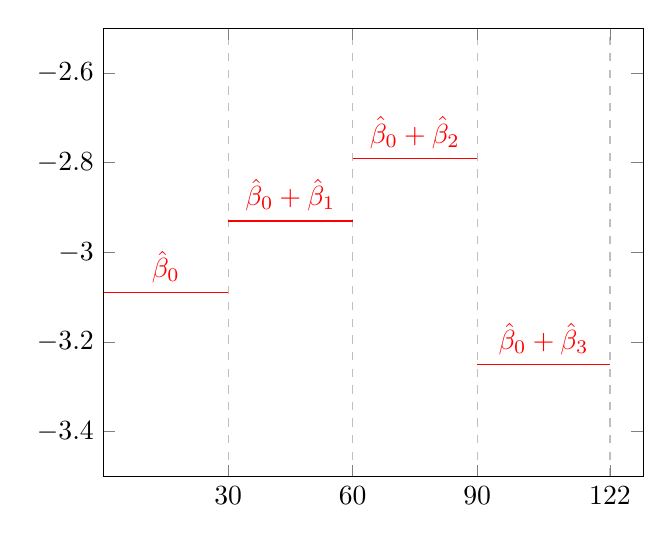
\begin{tikzpicture}
        \begin{axis}[
                xmin=0, xmax=130,
                ymin=-3.5, ymax=-2.5,
                xtick={30,60,90,122},
                legend pos=north west,
                ymajorgrids=false,
                xmajorgrids=true,
                grid style=dashed,
            ]
            \addplot[color=red] coordinates {(0,-3.09)(30,-3.09)} node [anchor=south,midway] (beta){$\hat{\beta}_0$} ;
            \addplot[color=red] coordinates {(30,-2.93)(60,-2.93)} node [anchor=south,midway] (beta){$\hat{\beta}_0+\hat{\beta}_1$};
            \addplot[color=red] coordinates {(60,-2.79)(90,-2.79)} node [anchor=south,midway] (beta){$\hat{\beta}_0+\hat{\beta}_2$};
            \addplot[color=red] coordinates {(90,-3.25)(122,-3.25)} node [anchor=south,midway] (beta){$\hat{\beta}_0+\hat{\beta}_3$};
        \end{axis}
    \end{tikzpicture}
\end{center}
\begin{itemize}
    \item $ \log{\hat{\lambda}_1}=\hat{\beta}_0=-3.09 $.
    \item $ \log{\hat{\lambda}_2}=\hat{\beta}_0+\hat{\beta}_1=-3.09+0.16=-2.93 $.
    \item $ \log{\hat{\lambda}_3}=\hat{\beta}_0+\hat{\beta}_2=-3.09+0.3=-2.79 $.
    \item $ \log{\hat{\lambda}_4}=\hat{\beta}_0+\hat{\beta}_3=-3.09-0.16=-3.25 $.
\end{itemize}
\subsubsection*{Interpretation of \texttt{pfitC}}
\[ \textcolor{Green}{\log{\mu_i}=\beta_0+\underbrace{\beta_1x_{i1}+\beta_2x_{i2}+\beta_3x_{i3}}_{\text{interval}}+\log{t_i}} \]
\begin{itemize}
    \item Relative Rate of events in interval 2 versus interval 1:
          \[ \exp{\beta_1}=\frac{\lambda(\text{interval 2})}{\lambda(\text{interval 1})}=\exp{0.16254}=1.176. \]
    \item Notice none of $ \beta_1,\beta_2,\beta_3 $ are statistically significant.
    \item There is a trend of a slightly higher rate in intervals 2 and 3 (versus interval 1) but
          the event rate does not differ significantly across follow-up time in the control rats.
\end{itemize}
\subsubsection*{2. Model Control and Treatment Groups (\texttt{pfit})}
\begin{itemize}
    \item Now, fit a model to both the treatment and control groups.
    \item $ x_{i4}=\Ind{\text{treatment group}} $.
    \item Assume a piecewise constant baseline rate function.
    \item Model is now:
          \[ \textcolor{Green}{\log{\mu_i}=\beta_0+\underbrace{\beta_1x_{i1}+\beta_2x_{i2}+\beta_3x_{i3}}_{\text{interval}}+\beta_4x_{i4}+\texttt{offset}(\log{t_i})}. \]
    \item $ \exp{\beta_1} $ is now RR of events for interval 2 versus interval 1, for two rats of the
          same treatment group.
\end{itemize}
%\begin{noindent}
\begin{knitrout}
\definecolor{shadecolor}{rgb}{0.969, 0.969, 0.969}\color{fgcolor}\begin{kframe}
\begin{alltt}
\hlstd{pfit} \hlkwb{<-} \hlkwd{glm}\hlstd{(count} \hlopt{~} \hlkwd{factor}\hlstd{(interval)} \hlopt{+} \hlstd{trt} \hlopt{+} \hlkwd{offset}\hlstd{(}\hlkwd{log}\hlstd{(len)),}
  \hlkwc{family} \hlstd{=} \hlkwd{poisson}\hlstd{(}\hlkwc{link} \hlstd{= log),} \hlkwc{data} \hlstd{= rats.pw)}
\hlkwd{summary}\hlstd{(pfit)}
\end{alltt}
\begin{verbatim}

Call:
glm(formula = count ~ factor(interval) + trt + offset(log(len)), 
    family = poisson(link = log), data = rats.pw)

Deviance Residuals: 
    Min       1Q   Median       3Q      Max  
-1.8335  -1.1994  -0.3302   0.4701   3.0551  

Coefficients:
                  Estimate Std. Error z value Pr(>|z|)    
(Intercept)       -3.08818    0.15079 -20.480  < 2e-16 ***
factor(interval)2  0.17185    0.19590   0.877    0.380    
factor(interval)3  0.20634    0.19438   1.062    0.288    
factor(interval)4 -0.06454    0.20412  -0.316    0.752    
trt               -0.82302    0.15171  -5.425 5.79e-08 ***
---
Signif. codes:  0 '***' 0.001 '**' 0.01 '*' 0.05 '.' 0.1 ' ' 1

(Dispersion parameter for poisson family taken to be 1)

    Null deviance: 301.37  on 191  degrees of freedom
Residual deviance: 266.32  on 187  degrees of freedom
AIC: 547.75

Number of Fisher Scoring iterations: 5
\end{verbatim}
\end{kframe}
\end{knitrout}
%\end{noindent}
\subsubsection*{Interpretation of \texttt{pfit}}
\begin{itemize}
    \item Relative Rate of events for treatment versus control rats:
          \[ \exp{\beta_4}=\frac{\lambda(\text{treatment})}{\lambda(\text{control})}=\exp{-0.8230}=0.44. \]
    \item Controlling for interval of follow-up, the rate of tumour development in treated rats
          in $0.44$ times that of control rats.
    \item That is, treatment looks beneficial.
    \item Notice that $ \beta_4 $ is statistically significant.
    \item $ \beta_1,\beta_2,\beta_3 $ are still not statistically significant.
    \item Consider do we really need to use a time non-homogeneous model for this data?
\end{itemize}
\subsubsection*{3. Time Homogeneous Model (\texttt{fit})}
\[ \textcolor{Green}{\log{\mu_i}=\beta_0+\beta_4x_{i4}+\log{t_i}}. \]
\begin{itemize}
    \item $ \beta_0= $ log rate of tumour development, per day, control group.
    \item $ \beta_4= $ log Relative Rate (RR) of tumour development in treated vs control rats.
    \item This model is nested within the time non-homogeneous model.
    \item Consider \texttt{pfit} model with $ \beta_1=\beta_2=\beta_3=0 $.
    \item We can carry out a likelihood ratio test
\end{itemize}
%\begin{noindent}
\begin{knitrout}
\definecolor{shadecolor}{rgb}{0.969, 0.969, 0.969}\color{fgcolor}\begin{kframe}
\begin{alltt}
\hlstd{fit} \hlkwb{<-} \hlkwd{glm}\hlstd{(count} \hlopt{~} \hlstd{trt} \hlopt{+} \hlkwd{offset}\hlstd{(}\hlkwd{log}\hlstd{(len)),} \hlkwc{family} \hlstd{=} \hlkwd{poisson}\hlstd{(}\hlkwc{link} \hlstd{= log),}
  \hlkwc{data} \hlstd{= rats.pw)}
\hlkwd{summary}\hlstd{(fit)}
\end{alltt}
\begin{verbatim}

Call:
glm(formula = count ~ trt + offset(log(len)), family = poisson(link = log), 
    data = rats.pw)

Deviance Residuals: 
    Min       1Q   Median       3Q      Max  
-1.7800  -1.1421  -0.4235   0.4009   3.2673  

Coefficients:
            Estimate Std. Error z value Pr(>|z|)    
(Intercept) -3.00562    0.08138 -36.934  < 2e-16 ***
trt         -0.82302    0.15171  -5.425 5.79e-08 ***
---
Signif. codes:  0 '***' 0.001 '**' 0.01 '*' 0.05 '.' 0.1 ' ' 1

(Dispersion parameter for poisson family taken to be 1)

    Null deviance: 301.37  on 191  degrees of freedom
Residual deviance: 269.06  on 190  degrees of freedom
AIC: 544.49

Number of Fisher Scoring iterations: 5
\end{verbatim}
\end{kframe}
\end{knitrout}
%\end{noindent}
\subsubsection*{Interpretation of \texttt{fit}}
\begin{itemize}
    \item Note $ \hat{\beta}_4=-0.8230 $ is almost unchanged versus model \texttt{fit}.
    \item Likelihood Ratio/Deviance test of $ \HN $: $ \beta_1=\beta_2=\beta_3=0 $:
          \[ \Delta D=D_0-D_A=269.060-266.323 \sim \chi^2_{3}\text{ under $\HN$}. \]
          %\begin{noindent}
\begin{knitrout}
\definecolor{shadecolor}{rgb}{0.969, 0.969, 0.969}\color{fgcolor}\begin{kframe}
\begin{alltt}
\hlnum{1} \hlopt{-} \hlkwd{pchisq}\hlstd{(fit}\hlopt{$}\hlstd{deviance} \hlopt{-} \hlstd{pfit}\hlopt{$}\hlstd{deviance, fit}\hlopt{$}\hlstd{df.residual} \hlopt{-} \hlstd{pfit}\hlopt{$}\hlstd{df.residual)}
\end{alltt}
\begin{verbatim}
[1] 0.4340077
\end{verbatim}
\end{kframe}
\end{knitrout}
    %\end{noindent}
    \item Do not reject $ \HN $.
    \item Conclude that the time homogeneous model (model 3) is probably OK in this case.
    \item However, we retain it for generality and for the following analysis.
\end{itemize}
\subsubsection*{4. Time Non-Homogeneous Model with Treatment Interaction (\texttt{ifit})}
\begin{itemize}
    \item Q: Is the treatment effect constant over time?
    \item Model with interaction:
          \textcolor{Green}{\begin{align*}
                  \log{\mu_i}
                   & =\beta_0+\overbrace{\beta_1x_{i1}+\beta_2x_{i2}+\beta_3x_{i3}}^{\text{interval}}+\overbrace{\beta_4x_{i4}}^{\text{treatment}}+ \\
                   & \quad +\underbrace{\beta_5x_{i1}x_{i4}+\beta_6x_{i2}x_{i4}+\beta_7x_{i3}x_{i4}}_{\text{interval$*$treatment}}+\log{t_i}
              \end{align*}}
    \item Model \texttt{pfit} (time non-homogeneous, without interaction) is nested within this
          model (consider \texttt{ifit} with $ \beta_5=\beta_6=\beta_7=0 $).
\end{itemize}
%\begin{noindent}
\begin{knitrout}
\definecolor{shadecolor}{rgb}{0.969, 0.969, 0.969}\color{fgcolor}\begin{kframe}
\begin{alltt}
\hlstd{ifit} \hlkwb{<-} \hlkwd{glm}\hlstd{(count} \hlopt{~} \hlkwd{offset}\hlstd{(}\hlkwd{log}\hlstd{(len))} \hlopt{+} \hlkwd{factor}\hlstd{(interval)} \hlopt{*} \hlstd{trt,}
  \hlkwc{family} \hlstd{=} \hlkwd{poisson}\hlstd{(}\hlkwc{link} \hlstd{= log),} \hlkwc{data} \hlstd{= rats.pw)}
\hlkwd{summary}\hlstd{(ifit)}
\end{alltt}
\begin{verbatim}

Call:
glm(formula = count ~ offset(log(len)) + factor(interval) * trt, 
    family = poisson(link = log), data = rats.pw)

Deviance Residuals: 
    Min       1Q   Median       3Q      Max  
-1.9183  -1.2158  -0.3241   0.5125   2.8959  

Coefficients:
                      Estimate Std. Error z value Pr(>|z|)    
(Intercept)           -3.09371    0.17150 -18.039   <2e-16 ***
factor(interval)2      0.16252    0.23326   0.697   0.4860    
factor(interval)3      0.30228    0.22617   1.337   0.1814    
factor(interval)4     -0.15691    0.24833  -0.632   0.5275    
trt                   -0.80392    0.31755  -2.532   0.0114 *  
factor(interval)2:trt  0.03164    0.42972   0.074   0.9413    
factor(interval)3:trt -0.37639    0.44663  -0.843   0.3994    
factor(interval)4:trt  0.28653    0.43808   0.654   0.5131    
---
Signif. codes:  0 '***' 0.001 '**' 0.01 '*' 0.05 '.' 0.1 ' ' 1

(Dispersion parameter for poisson family taken to be 1)

    Null deviance: 301.37  on 191  degrees of freedom
Residual deviance: 263.92  on 184  degrees of freedom
AIC: 551.35

Number of Fisher Scoring iterations: 5
\end{verbatim}
\end{kframe}
\end{knitrout}
%\end{noindent}
\subsubsection*{Interpretation of \texttt{ifit}}
\begin{itemize}
    \item Note $ \hat{\beta}_4=-0.8038 $ is very similar to \texttt{pfit}.
    \item Likelihood Ratio/Deviance test of $ \HN $: $ \beta_5=\beta_6=\beta_7=0 $:
          \[ \Delta D=D_0-D_A=266.323-263.917 \sim \chi^2_{3}\text{ under $\HN$}. \]
          %\begin{noindent}
\begin{knitrout}
\definecolor{shadecolor}{rgb}{0.969, 0.969, 0.969}\color{fgcolor}\begin{kframe}
\begin{alltt}
\hlnum{1} \hlopt{-} \hlkwd{pchisq}\hlstd{(pfit}\hlopt{$}\hlstd{deviance} \hlopt{-} \hlstd{ifit}\hlopt{$}\hlstd{deviance, pfit}\hlopt{$}\hlstd{df.residual} \hlopt{-}
  \hlstd{ifit}\hlopt{$}\hlstd{df.residual)}
\end{alltt}
\begin{verbatim}
[1] 0.4926145
\end{verbatim}
\end{kframe}
\end{knitrout}
            %\end{noindent}
    \item Do not reject $ \HN $.
    \item We do not have evidence that the treatment effect varies across the time intervals.
\end{itemize}
\subsubsection*{Summary of Rat Tumour Data Analysis}
\begin{itemize}
    \item Looks like a piecewise constant rate function is not necessary.
    \item The best model (of the ones we examined) is \texttt{fit}:
          \[ \textcolor{Green}{\log{\mu_i}=\beta_0+\beta_4x_{i4}+\log{t_i}}. \]
    \item \textcolor{Blue}{Interpretation}: The relative rate for tumour development in treated versus control
          rats is:
          \[ \exp{\hat{\beta}_4}=\exp{-0.822995}=0.439. \]
    \item That is, treatment is beneficial (treated rates get fewer tumours).
    \item \textcolor{Blue}{Prediction}: Expected number of tumours for a treated rat observed for 70 days?
          \[ \log{\hat{\mu}}=\hat{\beta}_0+\hat{\beta}_4+\log{70}=-3.00562-0.82302+\log{70}=0.41986. \]
          \[ \hat{\mu}=\exp{0.41986}=1.5217. \]
\end{itemize}

\section*{Topic 3d: Introduction of Contingency Tables}
\addcontentsline{toc}{section}{Topic 3d: Introduction of Contingency Tables}
\subsection*{Analysis of Contingency Tables}
\addcontentsline{toc}{subsection}{Analysis of Contingency Tables}
\begin{itemize}
      \item Contingency tables can be formed to display data when all variables are categorical.
      \item Below is a two-dimensional $ I\times J $ contingency table.
            \[ \begin{NiceArray}{c|ccccccc|c}[first-row,first-col]
                                                       &        & \Block{1-7}{\text{Factor $ W $}}                                                                                                        \\
                                                       &        & 1                                & 2             & 3             & \cdots & j             & \cdots & J                                  \\
                        \midrule
                        \Block{7-1}{\text{Factor $V$}} & 1      & y_{11}                           & y_{12}        & y_{13}        & \cdots & y_{1j}        & \cdots & y_{1J}        & y_{1\bullet}       \\
                                                       & 2      & y_{21}                           & y_{22}        & y_{23}        & \cdots & y_{2j}        & \cdots & y_{2J}        & y_{2\bullet}       \\
                                                       & 3      & y_{31}                           & y_{32}        & y_{33}        & \cdots & y_{3j}        & \cdots & y_{3J}        & y_{3\bullet}       \\
                                                       & \vdots & \vdots                           & \vdots        & \vdots        & \ddots & \vdots        & \ddots & \vdots        & \vdots             \\
                                                       & i      & y_{i1}                           & y_{i2}        & y_{i3}        & \cdots & y_{ij}        & \cdots & y_{iJ}        & y_{i\bullet}       \\
                                                       & \vdots & \vdots                           & \vdots        & \vdots        & \ddots & \vdots        & \ddots & \vdots        & \vdots             \\
                                                       & I      & y_{I1}                           & y_{I2}        & y_{I3}        & \cdots & y_{Ij}        & \cdots & y_{IJ}        & y_{I\bullet}       \\
                        \midrule
                                                       &        & y_{\bullet 1}                    & y_{\bullet 2} & y_{\bullet 3} & \cdots & y_{\bullet j} & \cdots & y_{\bullet J} & y_{\bullet\bullet}
                  \end{NiceArray}. \]
      \item $ I= $ Number of rows; $ J= $ Number of columns.
      \item \textcolor{Blue}{Row Totals}: $ y_{i\bullet}=\sum_{j=1}^{J}y_{ij} $.
      \item \textcolor{Blue}{Column Totals}: $ y_{\bullet j}=\sum_{i=1}^{I}y_{ij} $.
      \item \textcolor{Blue}{Grand Total}: $ y_{\bullet\bullet}=\sum_{i=1}^{I}\sum_{j=1}^{J}y_{ij} $.
      \item Want to assess the nature/significance of ANY associations between the variables.
      \item No special response variable --- all factors are of equal importance.
      \item Contingency tables are a cross-classification of units with respect to the factors of
            interest.
      \item The observations $ y_{ij} $ consist of all the cell counts of the contingency table --- these will be our ``responses.''
\end{itemize}
\subsubsection*{Example: 2-way Contingency Table}
\begin{Example}{Breast Self-Examination Contingency Table}
      \begin{itemize}
            \item Senie \emph{et al}. (1981) investigated the relationship between age and frequency of
                  breast self-examination in a sample of women.
            \item Two factors: Age (at 3 levels) and Frequency (at 3 levels).
                  \begin{center}
                        \begin{NiceTabular}{c|ccc|c}[first-row,first-col]
                              &&\Block{1-3}{Frequency of breast self-examination}\\
                              && Monthly & Occasionally & Never & Total\\
                              \midrule
                              \Block{3-1}{Age} & $<$45 & $ 91 $ & $ 90 $ & $ 51 $ & $ 232 $\\
                              & 45--59 & $ 150 $ & $ 200 $ & $ 155 $ & $ 505 $\\
                              & $ \ge $60 & $ 109 $ & $ 198 $ & $ 172 $ & $ 479 $\\
                              \midrule
                              & Total & $ 350 $ & $ 488 $ & $ 378 $ & $ 1216 $
                        \end{NiceTabular}
                  \end{center}
            \item Is than an association between age and exam frequency?
      \end{itemize}
\end{Example}
\subsubsection*{Basic Assumption in Contingency Tables}
\begin{itemize}
      \item \textcolor{Blue}{Basic Assumption}: Each cell count has an independent Poisson distribution with
            mean $ \mu_{ij} $ for the $ (i,j) $ cell
            \[ \Prob{Y_{ij}=y_{ij}}=\frac{\mu_{ij}^{y_{ij}}e^{-\mu_{ij}}}{y_{ij}!},\;y_{ij}=0,1,2,\ldots. \]
      \item The joint distribution is
            \[ \Prob{Y_{i j}=y_{i j}, i=1, \ldots, I, j=1, \ldots, J}=
                  \prod_{i=1}^{I} \prod_{j=1}^{J}\biggl(\frac{\mu_{i j}^{y_{i j}} e^{-\mu_{i j}}}{y_{i j} !}\biggr) \]
      \item We will condition on the relevant fixed totals (row, column, or grand) (possibly
            fixed by design) to get a multinomial or product multinomial distribution.
      \item Will show that these can all by analysed using Poisson GLMs.
\end{itemize}
\subsection*{The Multinomial Distribution}
\addcontentsline{toc}{subsection}{The Multinomial Distribution}
\begin{itemize}
      \item Assume the total number of units is fixed $ Y_{\bullet\bullet}=y_{\bullet\bullet} $ ($ =n $).
      \item Units are then cross-classified by $ 2 $ factors $ V $ and $ W $.
      \item Our assumption of $ Y_{ij}\sim \POI{\mu_{ij}} $ independently implies
            \[ Y_{\bullet\bullet}\sim \POI{\mu_{\bullet\bullet}},\text{ where }\mu_{\bullet\bullet}=\sum\sum \mu_{ij}. \]
      \item To get the joint distribution of the $ Y_{ij} $'s, we must condition on the grand total $ Y_{\bullet\bullet}=y_{\bullet\bullet} $
            since this is a fixed design:
            \begin{align*}
                  \Prob{Y_{ij}=y_{ij}\forall i,j\given Y_{\bullet\bullet}=y_{\bullet\bullet}}
                   & =\frac{\Prob{Y_{ij}=y_{ij}\forall i,j,Y_{\bullet\bullet}=y_{\bullet\bullet}}}{\Prob{Y_{\bullet\bullet}=y_{\bullet\bullet}}}                                           \\
                   & =\frac{\prod_{i=1}^{I} \prod_{j=1}^{J}\biggl(\frac{\mu_{i j}^{y_{i j}} \exp{-\mu_{i j}}}{y_{i j} !}\biggr)}{
                  \mu_{\bullet\bullet}^{y_{\bullet\bullet}}\exp{-\mu_{\bullet\bullet}}/y_{\bullet\bullet}!
                  }                                                                                                                                                                        \\
                   & =\biggl(\frac{y_{\bullet\bullet}!}{\prod\prod y_{ij}!}\biggr)\biggl(\frac{\prod\prod \mu_{ij}^{y_{ij}}}{\mu_{\bullet\bullet}^{y_{\bullet\bullet}}}\biggr)
                  \underbrace{\biggl(\frac{\exp*{-\sum\sum \mu_{ij}}}{\exp{-\mu_{\bullet\bullet}}}\biggr)}_{\textcolor{Green}{\text{$=1$ since $\mu_{\bullet\bullet}=\sum\sum \mu_{ij}$}}} \\
                   & =\biggl(\frac{y_{\bullet\bullet}!}{\prod\prod y_{ij}!}\biggr)
                  \underbrace{\prod_{i=1}^I \prod_{j=1}^J \biggl(\frac{\mu_{ij}}{\mu_{\bullet\bullet}}\biggr)^{\! y_{ij}}}_{\textcolor{Green}{\text{since $\mu_{\bullet\bullet}^{y_{\bullet\bullet}}=\mu_{\bullet\bullet}^{\sum\sum y_{ij}}=\prod\prod \mu_{\bullet\bullet}^{y_{ij}}$}}}
            \end{align*}
      \item Recall the standard \textcolor{Blue}{Multinomial distribution}:
            \[ f(x_1,\ldots,x_k;n,\pi_1,\ldots,\pi_k)=\Prob{X_1=x_1,\ldots,X_k=x_k}=\frac{n!}{x_1!\cdots x_k!}\pi_1^{x_1}\cdots \pi_k^{x_k}, \]
            where $ \sum \pi_i=1 $ and $ \sum x_i=n $.
      \item The pmf on the previous slide is a multinomial distribution with
            \[ \pi_{ij}=\mu_{ij}/\mu_{\bullet\bullet}=\Prob{\text{level $i$ of factor $V$ and level $j$ of factor $W$}}. \]
      \item Note that $\sum\sum \pi_{ij}=1$
            \[ \textcolor{Blue}{\Prob{Y_{ij}=y_{ij}\forall i,j\given Y_{\bullet\bullet}=y_{\bullet\bullet}}
                  =\biggl(\frac{y_{\bullet\bullet}!}{\prod\prod y_{ij}!}\biggr)\prod_{i=1}^I \prod_{j=1}^J \pi_{ij}^{y_{ij}}}. \]
\end{itemize}
\subsubsection*{Multinomial Likelihood}
\[ \Prob{Y_{ij}=y_{ij}\forall i,j\given Y_{\bullet\bullet}=y_{\bullet\bullet}}
      =\biggl(\frac{y_{\bullet\bullet}!}{\prod\prod y_{ij}!}\biggr)\prod_{i=1}^I \prod_{j=1}^J \pi_{ij}^{y_{ij}}. \]
\begin{itemize}
      \item $ \Vector{\pi}=(\pi_{11},\ldots,\pi_{IJ})^\top $ be the parameter vector.
      \item The likelihood and log-likelihood are given by:
            \[ L(\Vector{\pi})=\prod_i\prod_j \pi_{ij}^{y_{ij}},\text{ where }\sum\sum \pi_{ij}=1 \]
            \[ \ell(\Vector{\pi})=\sum_i\sum_j y_{ij}\log{\pi_{ij}}. \]
\end{itemize}
\subsubsection*{Testing for Independence in a 2-way Table}
\begin{itemize}
      \item Thinking back to the contingency table, we might be interested in testing the
            hypothesis that the two methods of classification are \textcolor{Blue}{independent}:
            \[ \HN\colon \pi_{ij}=\pi_{i\bullet}\pi_{\bullet j}\;\forall i,j \]
            \[ \HA\colon \pi_{ij}\ne \pi_{i\bullet}\pi_{\bullet j}\;\text{for some } i,j, \]
            where $ \pi_{i\bullet}=\sum_{j=1}^{J}\pi_{ij} $ and $ \pi_{\bullet j}=\sum_{i=1}^{I}\pi_{ij} $.
      \item Consider the log-likelihood \textcolor{Blue}{under $ \HN $ (independence)}:
            \begin{align*}
                  \ell(\Vector{\pi})
                   & =\sum_{i} \sum_{j} y_{i j} \log{\pi_{i\bullet} \pi_{\bullet j}}                             \\
                   & =\sum_{i} \sum_{j} y_{i j}\bigl(\log{\pi_{i\bullet}} +\log{\pi_{\bullet j}} \bigr)          \\
                   & =\sum_{i} y_{i \bullet} \log{\pi_{i \bullet}}+\sum_{j} y_{\bullet j} \log{\pi_{\bullet j}}.
            \end{align*}
      \item The parameters are constrained by $ \sum \pi_{i\bullet}=1 $ and $ \sum \pi_{\bullet j}=1 $.
      \item The MLEs of $ \pi_{i\bullet} $ and $ \pi_{\bullet j}  $ under $ \HN $ are:
            \[ \hat{\pi}_{i\bullet}=\frac{y_{i\bullet}}{y_{\bullet\bullet}},\qquad \hat{\pi}_{\bullet j}=\frac{y_{\bullet j}}{y_{\bullet\bullet}}. \]
      \item And the log-likelihood evaluated at the MLE is:
            \[ \ell(\hat{\Vector{\pi}})=\sum_{i} \sum_{j} y_{i j} \log*{\frac{y_{i \bullet} y_{\bullet j}}{y_{\bullet\bullet}^{2}}}. \]
      \item Next consider working \textcolor{Blue}{under $ \HA $ (unconstrained)}.
      \item The unconstrained MLEs are: $ \tilde{\pi}_{ij}=\frac{y_{ij}}{y_{\bullet\bullet}} $.
      \item And the log-likelihood evaluated at the unconstrained MLE is:
            \[ \ell(\tilde{\Vector{\pi}})=\sum_{i} \sum_{j} y_{i j} \log*{\frac{y_{ij}}{y_{\bullet\bullet}}}. \]
      \item To test for independence we could use a \textcolor{Blue}{Likelihood Ratio/Deviance} test for the
            multinomial:
            \begin{align*}
                  D
                   & =2\bigl(\ell(\tilde{\Vector{\pi}})-\ell(\hat{\Vector{\pi}})\bigr)                                                             \\
                   & =2\sum_i\sum_j y_{ij}\log*{\frac{y_{ij}}{y_{\bullet\bullet}}\bigg/\frac{y_{i \bullet} y_{\bullet j}}{y_{\bullet\bullet}^{2}}} \\
                   & =2\sum_i\sum_j y_{ij}\log*{\frac{y_{ij}}{y_{i\bullet}y_{\bullet j}/y_{\bullet\bullet}}}                                       \\
                   & =2\sum_i\sum_j O_{ij}\log*{\frac{O_{ij}}{E_{ij}}}.
            \end{align*}
      \item Note this has the usual form of a Deviance Statistic with
            \[ O_{ij}=y_{ij}\quad\text{ and }\quad E_{ij}=y_{\bullet\bullet}\hat{\pi}_{ij}\text{ under $ \HN $}. \]
      \item We know $ D \sim \chi^2_{n-p)} $, but what are the degrees of freedom here?
            \begin{align*}
                  n-p
                   & =(\text{\# parameters saturated})-(\text{\# parameters unsaturated}) \\
                   & =(IJ-1)-\bigl((I-1)+(J-1)\bigr)                                      \\
                   & =IJ-I-J+1                                                            \\
                   & =(I-1)(J-1).
            \end{align*}
\end{itemize}
\subsubsection*{Example: Breast Self-Examination Data ($ \tilde{\mu}_{ij} $ vs $ \hat{\mu}_{ij} $)}
\begin{itemize}
      \item \textcolor{Blue}{Observed Data}: $ y_{ij}=\tilde{\mu}_{ij}=\tilde{\pi}_{ij}y_{\bullet\bullet} $:
            \begin{table}[H]
                  \centering
                  \begin{NiceTabular}{c|ccc|c}[first-row,first-col]
                        &           & \Block{1-3}{Frequency of breast self-examination}                                     \\
                        &           & Monthly                                           & Occasionally & Never   & Total    \\
                        \midrule
                        \Block{3-1}{Age} & $<$45     & $ 91 $                                            & $ 90 $       & $ 51 $  & $ 232 $  \\
                        & 45--59    & $ 150 $                                           & $ 200 $      & $ 155 $ & $ 505 $  \\
                        & $ \ge $60 & $ 109 $                                           & $ 198 $      & $ 172 $ & $ 479 $  \\
                        \midrule
                        & Total     & $ 350 $                                           & $ 488 $      & $ 378 $ & $ 1216 $
                  \end{NiceTabular}
            \end{table}
      \item \textcolor{Blue}{Expected Data under $ \HN $}: $ \hat{\mu}_{ij}=\hat{\pi}_{ij}y_{\bullet\bullet}=y_{i\bullet}y_{\bullet j}/y_{\bullet\bullet} $:
            \begin{table}[H]
                  \centering
                  \begin{NiceTabular}{c|ccc|c}[first-row,first-col]
                        &           & \Block{1-3}{Frequency of breast self-examination}                                        \\
                        &           & Monthly                                           & Occasionally & Never      & Total    \\
                        \midrule
                        \Block{3-1}{Age} & $<$45     & $ 66.78 $                                         & $ 93.11 $    & $ 72.12 $  & $ 232 $  \\
                        & 45--59    & $ 145.35 $                                        & $ 202.66 $   & $ 156.98 $ & $ 505 $  \\
                        & $ \ge $60 & $ 137.87 $                                        & $ 192.23 $   & $ 148.90 $ & $ 479 $  \\
                        \midrule
                        & Total     & $ 350 $                                           & $ 488 $      & $ 378 $    & $ 1216 $
                  \end{NiceTabular}
            \end{table}
\end{itemize}
\subsubsection*{Example: Breast Self-Examination Data: ($ \tilde{\pi}_{ij} $ vs $ \hat{\pi}_{ij} $)}
\begin{itemize}
      \item \textcolor{Blue}{Unconstrained MLEs}: $ \tilde{\pi}_{ij}=y_{ij}/y_{\bullet\bullet} $ (as percentages):
            \begin{table}[H]
                  \centering
                  \begin{NiceTabular}{c|ccc|c}[first-row,first-col]
                        &           & \Block{1-3}{Frequency of breast self-examination}                                        \\
                        &           & Monthly                                           & Occasionally & Never      & Row \%    \\
                        \midrule
                        \Block{3-1}{Age} & $<$45     & $ 7.48 $                         & $ 7.40 $    & $ 4.19 $  & $ 19.07 $  \\
                        & 45--59                     & $ 12.34 $                       & $ 16.45 $   & $ 12.75 $ & $ 41.54 $  \\
                        & $ \ge $60                  & $ 8.96 $                       & $ 16.28 $   & $ 14.14 $ & $ 39.38 $  \\
                        \midrule
                        & Column \%                       & $ 28.78 $                         & $ 40.13 $      & $ 31.08 $    & $ 100 $
                  \end{NiceTabular}
            \end{table}
      \item \textcolor{Blue}{Constrained MLEs under $ \HN $}: $ \hat{\pi}_{ij}=\hat{\pi}_{i\bullet}\hat{\pi}_{\bullet j}=y_{i\bullet}y_{\bullet j}/y_{\bullet\bullet}^2 $:
            \begin{table}[H]
                  \centering
                  \begin{NiceTabular}{c|ccc|c}[first-row,first-col]
                        &           & \Block{1-3}{Frequency of breast self-examination}                                        \\
                        &           & Monthly                                           & Occasionally & Never      & Row \%    \\
                        \midrule
                        \Block{3-1}{Age} & $<$45     & $ 5.49 $                         & $ 7.66 $    & $ 5.93 $  & $ 19.08 $  \\
                        & 45--59                     & $ 11.95 $                       & $ 16.67 $   & $ 12.91 $ & $ 41.53 $  \\
                        & $ \ge $60                  & $ 11.34 $                       & $ 15.81 $   & $ 12.25 $ & $ 39.40 $  \\
                        \midrule
                        & Column \%                       & $ 28.78 $                         & $ 40.14  $      & $ 31.09 $    & $ 100 $
                  \end{NiceTabular}
            \end{table}
\end{itemize}
\subsubsection*{Example: Breast Self-Examination Data (Testing Independence)}
\begin{itemize}
      \item Use the Likelihood Ratio/Deviance test derived for the Multinomial Distribution
            \[ D=2\sum_i\sum_j y_{ij}\log*{\frac{y_{ij}}{y_{i\bullet}y_{\bullet j}/y_{\bullet\bullet}}}=25.19226. \]
      \item Compare to a $ \chi^2_{4} $ distribution:
            \[ p=\Prob*{\chi^2_{4}>25.19226}<0.001. \]
      \item So we reject the null hypothesis that age and frequency of breast self-examination
            are independent.
\end{itemize}
\subsection*{The Product Multinomial Distribution}
\addcontentsline{toc}{subsection}{The Product Multinomial Distribution}
\begin{itemize}
      \item Previously, we assumed the grand total $ Y_{\bullet\bullet}=y_{\bullet\bullet} $ was fixed.
      \item Now assume that the \textcolor{Blue}{row totals} $ Y_{i\bullet}=y_{i\bullet} $ are fixed.
            \begin{itemize}
                  \item Choose a sample of fixed size from populations $ i=1,\ldots,I $ and then classify the
                        units with response to Factor $W$.
            \end{itemize}
      \item Our assumption of $ Y_{ij}\sim \POI{\mu_{ij}} $ independently implies
            \[ Y_{i\bullet}\sim \POI{\mu_{i\bullet}},\text{ where }\mu_{i\bullet}=\sum_{j}\mu_{ij}. \]
      \item To get the joint distribution of the $ Y_{ij} $'s we now condition on the row totals
            $ Y_{i\bullet}=y_{i\bullet} $, $ i=1,\ldots,I $
            \[ \Prob{Y_{ij}=y_{ij}\forall i,j\given Y_{i\bullet}=y_{i\bullet}\forall i}
                  =\frac{\Prob{Y_{ij}=y_{ij}\forall i,j,Y_{i\bullet}=y_{i\bullet}\forall i}}{\Prob{Y_{i\bullet}=y_{i\bullet}\forall i}}.     \]
\end{itemize}
\subsubsection*{Example: Another Breast Self-Examination Study}
\begin{itemize}
      \item Imagine this time the investigators decided study a fixed number of women of
            each age group.
      \item The (hypothetical) 2-way contingency table is now:
            \begin{Example}{Breast Self-Examination Contingency Table (Hypothetical)}
                  \begin{center}
                        \begin{NiceTabular}{c|ccc|c}[first-row,first-col]
                              &&\Block{1-3}{Frequency of breast self-examination}\\
                              && Monthly & Occasionally & Never & Total\\
                              \midrule
                              \Block{3-1}{Age} & $<$45 & $ 78 $ & $ 78 $ & $ 44 $ & $ 200 $\\
                              & 45--59 & $ 178 $ & $ 238 $ & $ 184 $ & $ 600 $\\
                              & $ \ge $60 & $ 91 $ & $ 165 $ & $ 144 $ & $ 400 $\\
                              \midrule
                              & Total & $ 347 $ & $ 481 $ & $ 372 $ & $ 1200 $
                        \end{NiceTabular}
                  \end{center}
            \end{Example}
      \item We need to take this method of sampling into account in the analysis.
\end{itemize}
\begin{align*}
      \Prob{Y_{ij}=y_{ij}\forall i,j\given Y_{i\bullet}=y_{i\bullet}\forall i}
       & =\biggl(\prod_i \prod_j \biggl(\frac{\mu_{ij}^{y_{ij}} \exp{-\mu_{ij}}}{y_{ij}!}\biggr)\biggr)\Bigg/\biggl(\prod_i \frac{\mu_{i\bullet}^{y_{i\bullet}}\exp{-\mu_{i\bullet}}}{y_{i\bullet}!}\biggr)             \\
       & =\biggl(\frac{\prod_i y_{i\bullet}!}{\prod\prod y_{ij}!}\biggr)\biggl(\frac{\prod\prod \mu_{ij}^{y_{ij}}}{\prod_i \mu_{i\bullet}^{y_{i\bullet}}}\biggr)
      \underbrace{\biggl(\frac{\exp{-\sum\sum \mu_{ij}}}{\exp{-\sum_i \mu_i}}\biggr)}_{\textcolor{Green}{\text{$=1$ since $\mu_{i j}=\sum_i \mu_{i\bullet}=\mu_{\bullet\bullet}$ }}}                                    \\
       & =\prod_{i=1}^I \underbrace{\biggl(\frac{y_{i\bullet}!}{\prod_j y_{ij}!}\prod_{j=1}^J \biggl(\frac{\mu_{ij}}{\mu_{i\bullet}}\biggr)^{\!y_{ij}}\biggr)}_{\textcolor{Green}{\text{Multinomial pmf for row $i$}}}.
\end{align*}
\begin{itemize}
      \item This is the \textcolor{Blue}{product multinomial distribution} with $ \pi_{ij}=\mu_{ij}/\mu_{i\bullet} $.
      \item Here, $ \pi_{ij}= $ probability of being level $j$ given population level $i$.
      \item Note that $ \sum_j \pi_{ij}=1 $ for all $ i $.
\end{itemize}
\subsubsection*{Product Multinomial Likelihood}
\[ \Prob{Y_{ij}=y_{ij}\forall i,j\given Y_{i\bullet}=y_{i\bullet}\forall i}=
      \prod_{i=1}^I\biggl(\frac{y_{i\bullet}!}{\prod_j y_{ij}!}\prod_{j=1}^J \pi_{ij}^{y_{ij}}\biggr). \]
\begin{itemize}
      \item Again, let $ \Vector{\pi}=(\pi_{11},\ldots,\pi_{IJ})^\top $ be the parameter vector.
      \item Note the $ \pi_{ij} $ have different interpretations here versus the multinomial case.
      \item The log-likelihood is given by:
            \[ \ell(\Vector{\pi})=\sum_i\sum_j y_{ij}\log{\pi_{ij}},\text{ where }\sum_j \pi_{ij}=1\;\forall i. \]
\end{itemize}
\subsubsection*{Testing for Independence with the Product Multinomial}
\begin{itemize}
      \item In this case we might be interested in testing where the probability of being at
            factor level $j$ is the same across all stratum/populations $ i=1,\ldots,I $
            \[ \HN\colon \pi_{1j}=\pi_{2j}=\cdots=\pi_{Ij}=\pi_j,\;j=1,2,\ldots,J, \]
            \[ \HA\colon \text{at least one }\pi_{ij}\ne \pi_{i^\prime j}. \]
      \item The log likelihood \textcolor{Blue}{under $ \HN $ (independence)} is
            \[ \ell(\Vector{\pi})=\sum_i\sum_j y_{ij}\log{\pi_{j}}=\sum_j y_{\bullet j}\log{\pi_{j}}. \]
      \item The parameters are constrained by $ \sum_{j}\pi_j=1 $.
      \item The MLEs under $ \HN $ are
            \[ \hat{\pi}_{ij}=\hat{\pi}_j=\frac{y_{\bullet j}}{y_{\bullet\bullet}}. \]
      \item \textcolor{Blue}{Under $ \HA $ (unconstrained)} the MLEs are
            \[ \tilde{\pi}_{ij}=\frac{y_{ij}}{y_{i\bullet}}. \]
      \item The \textcolor{Blue}{Likelihood Ratio/Deviance} test statistic is:
            \begin{align*}
                  D
                   & =2\bigl(\ell(\tilde{\Vector{\pi}})-\ell(\hat{\Vector{\pi}})\bigr)                                     \\
                   & =2\sum_i\sum_j y_{ij}\log*{\frac{y_{ij}}{y_{i\bullet}}\bigg/\frac{y_{\bullet j}}{y_{\bullet\bullet}}} \\
                   & =2\sum_i\sum_j y_{ij}\log*{\frac{y_{ij}}{y_{i\bullet}y_{\bullet j}/y_{\bullet\bullet}}}.
            \end{align*}
      \item Which is identical to the Deviance statistic for testing independence under a
            multinomial distribution.
      \item Here, $ D \sim \chi^2_{(I-1)(J-1)} $ since
            \[ n-p=I(J-1)-(J-1)=IJ-I-J+1=(I-1)(J-1). \]
\end{itemize}
\subsubsection*{Example: Another Breast Self-Examination Study}
\begin{itemize}
      \item \textcolor{Blue}{Observed Data}: $ y_{ij} $:
            \begin{table}[H]
                  \centering
                  \begin{NiceTabular}{c|ccc|c}[first-row,first-col]
                        &&\Block{1-3}{Frequency of breast self-examination}\\
                        && Monthly & Occasionally & Never & Total\\
                        \midrule
                        \Block{3-1}{Age} & $<$45 & $ 78 $ & $ 78 $ & $ 44 $ & $ 200 $\\
                        & 45--59 & $ 178 $ & $ 238 $ & $ 184 $ & $ 600 $\\
                        & $ \ge $60 & $ 91 $ & $ 165 $ & $ 144 $ & $ 400 $\\
                        \midrule
                        & Total & $ 347 $ & $ 481 $ & $ 372 $ & $ 1200 $
                  \end{NiceTabular}
            \end{table}
      \item \textcolor{Blue}{Expected Data under $ \HN $}: $ \hat{\mu}_{ij}=y_{i\bullet}\hat{\pi}_j=y_{i\bullet}y_{\bullet j}/y_{\bullet\bullet} $
            \begin{table}[H]
                  \centering
                  \begin{NiceTabular}{c|ccc|c}[first-row,first-col]
                        &&\Block{1-3}{Frequency of breast self-examination}\\
                        && Monthly & Occasionally & Never & Total\\
                        \midrule
                        \Block{3-1}{Age} & $<$45 & $ 57.83 $ & $ 80.17 $ & $ 62.00 $ & $ 200 $\\
                        & 45--59 & $ 173.50 $ & $ 240.50 $ & $ 186.00 $ & $ 600 $\\
                        & $ \ge $60 & $ 115.67 $ & $ 160.33 $ & $ 124.00 $ & $ 400 $\\
                        \midrule
                        & Total & $ 347 $ & $ 481 $ & $ 372 $ & $ 1200 $
                  \end{NiceTabular}
            \end{table}
      \item \textcolor{Blue}{Unconstrained MLEs}: $ \tilde{\pi}_{ij}=y_{ij}/y_{i\bullet} $ (as percentages):
            \begin{table}[H]
                  \centering
                  \begin{NiceTabular}{c|ccc|c}[first-row,first-col]
                        &&\Block{1-3}{Frequency of breast self-examination}\\
                        && Monthly & Occasionally & Never & Total\\
                        \midrule
                        \Block{3-1}{Age} & $<$45 & $ 39.00 $ & $ 39.00 $ & $ 22.00 $ & $ 100 $\\
                        & 45--59 & $ 29.67 $ & $ 39.67 $ & $ 30.67 $ & $ 100 $\\
                        & $ \ge $60 & $ 22.75 $ & $ 41.25 $ & $ 36.00 $ & $ 100 $\\
                        \bottomrule
                  \end{NiceTabular}
            \end{table}
      \item \textcolor{Blue}{Constrained MLEs}: $ \hat{\pi}_{ij}=\hat{\pi}_j=y_{\bullet j}/y_{\bullet\bullet} $ (as percentages):
            \begin{table}[H]
                  \centering
                  \begin{NiceTabular}{c|ccc|c}[first-row,first-col]
                        &&\Block{1-3}{Frequency of breast self-examination}\\
                        && Monthly & Occasionally & Never & Total\\
                        \midrule
                        \Block{3-1}{Age} & $<$45 & $ 28.92 $ & $ 40.08 $ & $ 31.00 $ & $ 100 $\\
                        & 45--59 & $ 28.92 $ & $ 40.08 $ & $ 31.00 $ & $ 100 $\\
                        & $ \ge $60 & $ 28.92 $ & $ 40.08 $ & $ 31.00 $ & $ 100 $\\
                        \bottomrule
                  \end{NiceTabular}
            \end{table}
\end{itemize}
\subsubsection*{Example: Another Breast Self-Examination Study (Testing Independence)}
\begin{itemize}
      \item Use the Likelihood Ratio/Deviance test derived for the Multinomial Distribution
            \[ D=2\sum_i\sum_j y_{ij}\log*{\frac{y_{ij}}{y_{i\bullet}y_{\bullet j}/y_{\bullet\bullet}}}=21.25615. \]
      \item Compare to a $ \chi^2_{4} $ distribution:
            \[ p=\Prob*{\chi^2_{4}>21.25615}<0.001. \]
      \item So we reject the null hypothesis that age and frequency of breast self-examination
            are independent.
\end{itemize}
\subsubsection*{Summary}
\begin{itemize}
      \item Today we considered simple 2-way contingency tables.
      \item With the basic Poisson assumption for the cell counts, depending on the type of
            sampling used, we can test for independence using:
            \begin{enumerate}[1.]
                  \item Multinomial distribution (condition on $ y_{\bullet\bullet} $).
                  \item Product multinomial (condition on $ y_{i\bullet} $, $ i=1,2,\ldots,I $).
            \end{enumerate}
      \item Both yield the same Likelihood Ratio/Deviance test statistic.
      \item Interestingly we can also use log-linear models to assess these independence
            hypotheses (next week).
      \item Easily generalizable to 3-way (and more) contingency tables.
\end{itemize}

\makeheading{Week 10}{\daterange{2021-11-08}{2021-11-12}}
\section*{Topic 3e: Log Linear Models for Two-way Tables}
\addcontentsline{toc}{section}{Topic 3e: Log Linear Models for Two-way Tables}
\subsubsection*{Likelihood Based Analysis of 2-way Contingency Tables}
\[ \begin{NiceArray}{c|ccccccc|c}[first-row,first-col]
                                           &        & \Block{1-7}{\text{Factor $ W $}}                                                                                                        \\
                                           &        & 1                                & 2             & 3             & \cdots & j             & \cdots & J                                  \\
            \midrule
            \Block{7-1}{\text{Factor $V$}} & 1      & y_{11}                           & y_{12}        & y_{13}        & \cdots & y_{1j}        & \cdots & y_{1J}        & y_{1\bullet}       \\
                                           & 2      & y_{21}                           & y_{22}        & y_{23}        & \cdots & y_{2j}        & \cdots & y_{2J}        & y_{2\bullet}       \\
                                           & 3      & y_{31}                           & y_{32}        & y_{33}        & \cdots & y_{3j}        & \cdots & y_{3J}        & y_{3\bullet}       \\
                                           & \vdots & \vdots                           & \vdots        & \vdots        & \ddots & \vdots        & \ddots & \vdots        & \vdots             \\
                                           & i      & y_{i1}                           & y_{i2}        & y_{i3}        & \cdots & y_{ij}        & \cdots & y_{iJ}        & y_{i\bullet}       \\
                                           & \vdots & \vdots                           & \vdots        & \vdots        & \ddots & \vdots        & \ddots & \vdots        & \vdots             \\
                                           & I      & y_{I1}                           & y_{I2}        & y_{I3}        & \cdots & y_{Ij}        & \cdots & y_{IJ}        & y_{I\bullet}       \\
            \midrule
                                           &        & y_{\bullet 1}                    & y_{\bullet 2} & y_{\bullet 3} & \cdots & y_{\bullet j} & \cdots & y_{\bullet J} & y_{\bullet\bullet}
      \end{NiceArray}. \]
\begin{itemize}
      \item Previously: Previously: Derived Likelihood Ratio/Deviance tests for testing for \textcolor{Blue}{independence}
            between Factor $V$ and Factor $W$.
      \item \textcolor{Blue}{Basic Assumption}: $ Y_{ij} \sim \POI{\mu_{ij}} $, $ \forall i,j $.
      \item When we condition on the Grand Total the joint distribution becomes Multinomial,
            and we want to test:
            \[ \HN\colon \pi_{ij}=\pi_{i\bullet}\pi_{\bullet j}\;\forall i,j \]
            \[ \HA\colon \pi_{ij}\ne \pi_{i\bullet}\pi_{\bullet j}\;\text{for some } i,j. \]
      \item When we condition on the Row Totals the joint distribution becomes \textcolor{Blue}{Product
                  Multinomial}, and we want to test:
            \[ \HN\colon \pi_{1j}=\pi_{2j}=\cdots=\pi_{Ij}=\pi_j,\;j=1,2,\ldots,J, \]
            \[ \HA\colon \text{at least one }\pi_{ij}\ne \pi_{i^\prime j}. \]
      \item In either case, the \textcolor{Blue}{Likelihood Ratio/Deviance Test} statistic is:
            \[ D=2\sum_i\sum_j y_{ij}\log*{\frac{y_{ij}}{y_{i\bullet}y_{\bullet j}/y_{\bullet\bullet}}} \sim \chi^2_{(I-1)(J-1)}\text{ under $ \HN $}.\]
\end{itemize}
\subsection*{Log Linear Models for 2-way Contingency Tables}
\addcontentsline{toc}{subsection}{Log Linear Models for 2-way Tables}
\begin{itemize}
      \item \textcolor{Blue}{Basic Assumption}: $ Y_{ij} \sim \POI{\mu_{ij}} $, $ \forall i,j $.
      \item \textcolor{Blue}{Explanatory Variables}: Factor $V$ and $W$:
            \[ \begin{array}{cc}
                        \begin{aligned}
                              x_1     & =\Ind{\text{Factor $V$ at level 2}}, \\
                              x_2     & =\Ind{\text{Factor $V$ at level 3}}, \\
                                      & \vdotswithin{=}                      \\
                              x_{I-1} & =\Ind{\text{Factor $V$ at level I}}, \\
                        \end{aligned} &
                        \begin{aligned}
                              x_I       & =\Ind{\text{Factor $W$ at level 2}}, \\
                              x_{I+1}   & =\Ind{\text{Factor $W$ at level 3}}, \\
                                        & \vdotswithin{=}                      \\
                              x_{I+J-2} & =\Ind{\text{Factor $W$ at level J}}. \\
                        \end{aligned}
                  \end{array} \]
      \item The main effects log-linear model would be:
            \begin{align*}
                  \log{\mu_\ell}
                   & =\beta_0+\overbrace{\beta_1x_{1\ell}+\beta_2x_{2\ell}+\cdots+\beta_{I-1}x_{I-1\ell}}^{\text{Factor $V$}}+                               \\
                   & \quad+\underbrace{\beta_Ix_{I\ell}+\beta_{I+1}x_{I+1\ell}+\cdots+\beta_{I+J-2}x_{I+J-2\ell}}_{\text{Factor $W$}} &  & \ell=1,\ldots,IJ.
            \end{align*}
      \item Note: $ \text{\# parameters}=1+(I-1)+(J-1)=I+J-1 $.
      \item The $ \Vector{x}^\top \Vector{\beta} $ is quite cumbersome when $ I $ and $ J $ are large.
      \item Consider the following expression for the model:
            \[ \log{\mu_{ij}}=u+u_i^V+u_j^W,\;i=1,\ldots,I,\,j=1,\ldots,J, \]
            where $ u_1^V+u_1^W=0 $.
      \item Note: $ \text{\# parameters}=1+(I-1)+(J-1)=I+J-1 $.
      \item This notation suppresses the binary $ x $ variables.
      \item The relationship between the $ \beta $ and $ u $ is as follows:
            \[ \begin{array}{ccc}
                        u=\beta_0,                 &
                        \begin{aligned}
                              u_2^V & =\beta_1,       \\
                              u_3^V & =\beta_2,       \\
                                    & \vdotswithin{=} \\
                              u_I^V & =\beta_{I-1},
                        \end{aligned} &
                        \begin{aligned}
                              u_2^W & =\beta_I,       \\
                              u_3^W & =\beta_{I+1},   \\
                                    & \vdotswithin{=} \\
                              u_J^W & =\beta_{I+J-2}.
                        \end{aligned}
                  \end{array} \]
      \item Testing independence in a 2-way table:
            \[ \HN\colon \pi_{ij}=\pi_{i\bullet}\pi_{\bullet j}\;\forall i,j \]
            \[ \HA\colon \pi_{ij}\ne \pi_{i\bullet}\pi_{\bullet j}\;\text{for some } i,j. \]
      \item The corresponding log-linear models are:
            \[ \HN\colon \log{\mu_{ij}}=u+u_i^V+u_j^W \]
            \[ \HA\colon\log{\mu_{ij}}=u+u_i^V+u_j^W+u_{ij}^{VW}. \]
      \item Using \textcolor{Blue}{corner-point constraints} we require:
            \[ u_1^V=0,\qquad u_1^W=0,\qquad u_{1j}^{VW}=0\;\forall j,\qquad u_{i1}^{VW}\;\forall i. \]
      \item The interaction model has $ 1+(I-1)+(J-1)+(I-1)(J-1)=IJ $ parameters.
      \item \textcolor{Red}{Wait}: We're using a \textcolor{Blue}{Poisson} model to fit data/test hypotheses from a \textcolor{Blue}{Multinomial} distribution?
      \item Examine the log-likelihood from the Poisson:
            \[ \ell(\Vector{\mu})=\sum_i\sum_j\bigl[y_{ij}\log{\mu_{ij}}-\mu_{ij}-\log{y_{ij}!}\bigr]. \]
      \item Substitute in the log linear model \textcolor{Blue}{$ \HN\colon \log{\mu_{ij}}=u+u_i^V+u_j^W $}:
            \begin{align*}
                  \ell(\Vector{u})
                                & =\sum\sum\bigl(y_{ij}(\textcolor{Blue}{u+u_i^V+u_j^W})-\exp{\textcolor{Blue}{u+u_i^V+u_j^W}}-\log{y_{ij}!}\bigr)          \\
                  \pdv{\ell}{u} & =\sum\sum\bigl(y_{ij}-\exp{u+u_i^V+u_j^W}\bigr)                                                                           \\
                                & =\sum\sum(y_{ij}-\mu_{ij})                                                                                                \\
                                & =y_{\bullet\bullet}-\mu_{\bullet\bullet}\qquad \text{(set $=0$)}\implies \hat{\mu}_{\bullet\bullet}=y_{\bullet\bullet}.   \\
                  \pdv{\ell}{u_{i^\star}^V}
                                & =\sum\sum\bigl(y_{i^\star j}-\exp{u+u_{i^\star}^V+u_j^W}\bigr)                                                            \\
                                & =y_{i^\star\bullet}-\mu_{i^\star\bullet}\qquad \text{(set $=0$)}\implies\hat{\mu}_{i\bullet}=y_{i\bullet}\;\forall i.     \\
                  \pdv{\ell}{u_{j^\star}^W}
                                & =\sum\sum\bigl(y_{ij^\star}-\exp{u+u_{i}^V+u_{j^\star}^W}\bigr)                                                           \\
                                & =y_{\bullet j^\star}-\mu_{\bullet j^\star}\qquad \text{(set $=0$)}\implies\hat{\mu}_{\bullet j}=y_{\bullet j}\;\forall j.
            \end{align*}
      \item So the main effects log linear model reproduces the row, column and grand totals.
      \item If we do the same with the saturated model
            \[ \HA\colon\log{\mu_{ij}}=u+u_i^V+u_j^W+u_{ij}^{VW}, \]
            we find it provides a perfect fit to the data: $ \tilde{\mu}_{ij}=y_{ij} $ for all $ i,j $.
      \item Recall the Deviance Test for the Poisson Distribution
            \begin{align*}
                  D
                   & =2\bigl(\ell(\tilde{\Vector{\mu}})-\ell(\hat{\Vector{\mu}})\bigr)                                                                                                   \\
                   & =2\sum\sum\Bigl(\bigl(y_{ij}-\log{\tilde{\mu}_{ij}}-\tilde{\mu}_{ij}-\log{y_{ij}!}\bigr)-\bigl(y_{ij}-\log{\hat{\mu}_{ij}}-\hat{\mu}_{ij}-\log{y_{ij}!}\bigr)\Bigr) \\
                   & =2\sum\sum\biggl(y_{ij}\log*{\frac{\tilde{\mu}_{ij}}{\hat{\mu}_{ij}}}-(\tilde{\mu}_{ij}-\hat{\mu}_{ij})\biggr)                                                      \\
                   & =2\sum\sum y_{ij}\log*{\frac{y_{ij}}{y_{i\bullet}y_{\bullet j}/y_{\bullet\bullet}}},
            \end{align*}
            since
            \begin{align*}
                  \hat{\mu}_{ij}
                   & =y_{\bullet\bullet}\hat{\pi}_{i\bullet}\hat{\pi}_{\bullet j}                                                                                                   \\
                   & =y_{\bullet\bullet}\biggl(\frac{\hat{\mu}_{i\bullet}}{\hat{\mu}_{\bullet\bullet}}\biggr)\biggl(\frac{\hat{\mu}_{\bullet j}}{\hat{\mu}_{\bullet\bullet}}\biggr) \\
                   & =y_{i\bullet}y_{\bullet j}/y_{\bullet\bullet},
            \end{align*}
            and
            \begin{align*}
                  \sum\sum\tilde{\mu}_{ij} & =\sum\sum u_{ij}=y_{\bullet\bullet},            \\
                  \sum\sum\hat{\mu}_{ij}   & =\hat{\mu}_{\bullet\bullet}=y_{\bullet\bullet}.
            \end{align*}
            \[ D=2\sum\sum y_{ij}\log*{\frac{y_{ij}}{y_{i\bullet}y_{\bullet j}/y_{\bullet\bullet}}}. \]
      \item We know $ D \sim \chi^2_{n-p} $ under $ \HN $. Here,
            \[ n-p=(I-J)-\bigl(1+(I-1)+(J-1)\bigr)=(I-1)(J-1). \]
      \item Same as the Likelihood Ratio/Deviance Test statistic from the \textcolor{Blue}{Multinomial} and
            \textcolor{Blue}{Product Multinomial} last section.
      \item Use the Deviance Test from fitting \textcolor{Blue}{Poisson} models to conduct hypotheses tests
            for data from 2-way contingency tables!
\end{itemize}
\subsection*{Example: A Melanoma Study}
\addcontentsline{toc}{subsection}{Example: A Melanoma Study}
\begin{itemize}
      \item A cross-sectional study was conducted in which 400 patients with malignant
            melanoma were classified according to two factors: the \textcolor{Blue}{site of the tumour} and the
            \textcolor{Blue}{histological type}.
            \begin{Example}{Melanoma Study Data}
                  \begin{center}
                        \begin{tabular}{lcccc}
                              Tumour Type           & Head and Neck & Trunk & Extremities & Total \\
                              \midrule
                              Hutchinson's freckle  & 22            & 2     & 10          & 34    \\
                              Superficial Spreading & 16            & 54    & 115         & 185   \\
                              Nodular               & 19            & 33    & 73          & 125   \\
                              Indeterminate         & 11            & 17    & 28          & 56    \\
                              Total                 & 68            & 106   & 226         & 400
                        \end{tabular}
                  \end{center}
            \end{Example}
      \item Here we wish to investigate whether the different types of tumour appear equally
            likely in the different sites.
      \item That is, we are assessing \textcolor{Green}{whether there is an association between
                  histological type and tumour site}.
      \item We wish to test for \textcolor{Blue}{independence}:
            \[ \HN\colon \pi_{ij}=\pi_{i\bullet}\pi_{\bullet j}\;\forall i,j \]
            \[ \HA\colon \pi_{ij}\ne \pi_{i\bullet}\pi_{\bullet j}\;\text{for some } i,j. \]
      \item Under $ \HN $: $ \mu_{ij}=\E{Y_{ij}}=y_{\bullet\bullet}\pi_{i\bullet}\pi_{\bullet j} $, meaning we will have to fit the row and
            column totals to allow estimation of $ \pi_{i\bullet} $ and $ \pi_{\bullet j} $.
      \item Thus, our log linear model under the null hypothesis is
            \[ \log{\mu_{ij}}=u+u_i^V+u_j^W,\; i=1,2,3,4,\,j=1,2,3 \]
      \item $V$ corresponds to tumour type variable ($i$ indicating the level).
      \item $W$ corresponds to tumour site variable ($j$ indicating the level).
      \item \textcolor{Blue}{If the model fits the data well, then there's no evidence against the assumption
                  that tumour type and site are independent}.
      \item If the model does not fit the data well, then some tumour types appear more
            frequently in certain locations.
\end{itemize}
\subsubsection*{R Dataset}
\begin{Example}{Melanoma Data Set}
      % \begin{noindent}
\begin{knitrout}
\definecolor{shadecolor}{rgb}{0.969, 0.969, 0.969}\color{fgcolor}\begin{kframe}
\begin{verbatim}
   type locat   y
1     1     1  22
2     1     2   2
3     1     3  10
4     2     1  16
5     2     2  54
6     2     3 115
7     3     1  19
8     3     2  33
9     3     3  73
10    4     1  11
11    4     2  17
12    4     3  28
\end{verbatim}
\end{kframe}
\end{knitrout}
% \end{noindent}
\end{Example}
\subsubsection*{R Code}
%\begin{noindent}
\begin{knitrout}
\definecolor{shadecolor}{rgb}{0.969, 0.969, 0.969}\color{fgcolor}\begin{kframe}
\begin{alltt}
\hlstd{derm.dat} \hlkwb{=} \hlkwd{read.table}\hlstd{(}\hlstr{"derm.dat"}\hlstd{,} \hlkwc{header} \hlstd{= T)}
\hlstd{derm.dat}\hlopt{$}\hlstd{typef} \hlkwb{=} \hlkwd{factor}\hlstd{(derm.dat}\hlopt{$}\hlstd{type)}
\hlstd{derm.dat}\hlopt{$}\hlstd{sitef} \hlkwb{=} \hlkwd{factor}\hlstd{(derm.dat}\hlopt{$}\hlstd{locat)}
\hlstd{derm.dat}
\hlcom{# fitting the model with both main effects}
\hlstd{model1} \hlkwb{=} \hlkwd{glm}\hlstd{(y} \hlopt{~} \hlstd{typef} \hlopt{+} \hlstd{sitef,} \hlkwc{family} \hlstd{= poisson,} \hlkwc{data} \hlstd{= derm.dat)}
\hlkwd{summary}\hlstd{(model1)}
\hlcom{# creating deviance residuals for diagnostic plots}
\hlstd{derm.dat}\hlopt{$}\hlstd{fitted.values} \hlkwb{=} \hlstd{model1}\hlopt{$}\hlstd{fitted.values}
\hlstd{derm.dat}\hlopt{$}\hlstd{rdeviance} \hlkwb{=} \hlkwd{residuals.glm}\hlstd{(model1,} \hlkwc{type} \hlstd{=} \hlstr{"deviance"}\hlstd{)}
\hlstd{derm.dat}
\hlcom{# fitting the model with only the 'histological type' main}
\hlcom{# effect}
\hlstd{model2} \hlkwb{=} \hlkwd{glm}\hlstd{(y} \hlopt{~} \hlstd{typef,} \hlkwc{family} \hlstd{= poisson,} \hlkwc{data} \hlstd{= derm.dat)}
\hlnum{1} \hlopt{-} \hlkwd{pchisq}\hlstd{(model2}\hlopt{$}\hlstd{deviance} \hlopt{-} \hlstd{model1}\hlopt{$}\hlstd{deviance, model2}\hlopt{$}\hlstd{df.residual} \hlopt{-}
  \hlstd{model1}\hlopt{$}\hlstd{df.residual)}
\hlcom{# fitting the model with only the 'site' main effect}
\hlstd{model3} \hlkwb{=} \hlkwd{glm}\hlstd{(y} \hlopt{~} \hlstd{sitef,} \hlkwc{family} \hlstd{= poisson,} \hlkwc{data} \hlstd{= derm.dat)}
\hlnum{1} \hlopt{-} \hlkwd{pchisq}\hlstd{(model3}\hlopt{$}\hlstd{deviance} \hlopt{-} \hlstd{model1}\hlopt{$}\hlstd{deviance, model3}\hlopt{$}\hlstd{df.residual} \hlopt{-}
  \hlstd{model1}\hlopt{$}\hlstd{df.residual)}
\end{alltt}
\end{kframe}
\end{knitrout}
%\end{noindent}
\begin{itemize}
      \item One line per cell in the contingency table.
      \item $IJ = 12$ observations.
      \item \texttt{type} is tumour type (4 levels).
      \item \texttt{locat} is tumour location (3 levels).
      \item \texttt{y} is the count in the contingency table.
\end{itemize}
\subsubsection*{R output for Model 1: \texttt{type + site}}
%\begin{noindent}
\begin{knitrout}
\definecolor{shadecolor}{rgb}{0.969, 0.969, 0.969}\color{fgcolor}\begin{kframe}
\begin{alltt}
\hlstd{model1} \hlkwb{=} \hlkwd{glm}\hlstd{(y} \hlopt{~} \hlstd{typef} \hlopt{+} \hlstd{sitef,} \hlkwc{family} \hlstd{= poisson,} \hlkwc{data} \hlstd{= derm.dat)}
\hlkwd{summary}\hlstd{(model1)}
\end{alltt}
\begin{verbatim}

Call:
glm(formula = y ~ typef + sitef, family = poisson, data = derm.dat)

Deviance Residuals: 
    Min       1Q   Median       3Q      Max  
-3.0453  -1.0741   0.1297   0.5857   5.1354  

Coefficients:
            Estimate Std. Error z value Pr(>|z|)    
(Intercept)   1.7544     0.2040   8.600  < 2e-16 ***
typef2        1.6940     0.1866   9.079  < 2e-16 ***
typef3        1.3020     0.1934   6.731 1.68e-11 ***
typef4        0.4990     0.2174   2.295  0.02173 *  
sitef2        0.4439     0.1554   2.857  0.00427 ** 
sitef3        1.2010     0.1383   8.683  < 2e-16 ***
---
Signif. codes:  0 '***' 0.001 '**' 0.01 '*' 0.05 '.' 0.1 ' ' 1

(Dispersion parameter for poisson family taken to be 1)

    Null deviance: 295.203  on 11  degrees of freedom
Residual deviance:  51.795  on  6  degrees of freedom
AIC: 122.91

Number of Fisher Scoring iterations: 5
\end{verbatim}
\end{kframe}
\end{knitrout}
%\end{noindent}
\begin{itemize}
      \item Recall we are testing for \textcolor{Blue}{independence}
            \[ \HN\colon \pi_{ij}=\pi_{i\bullet}\pi_{\bullet j}\;\forall i,j \]
            \[ \HA\colon \pi_{ij}\ne \pi_{i\bullet}\pi_{\bullet j}\;\text{for some } i,j. \]
      \item The Deviance test statistic $ \chi^2_{12-6} $ under $ \HN $.
      \item Here $ D=51.795 $ which corresponds to a $ p $-value of
            \[ p=\Prob*{\chi^2_{6}>51.795}<0.001. \]
            Therefore, we reject the null hypothesis of independence.
            %\begin{noindent}
\begin{knitrout}
\definecolor{shadecolor}{rgb}{0.969, 0.969, 0.969}\color{fgcolor}\begin{kframe}
\begin{alltt}
\hlnum{1} \hlopt{-} \hlkwd{pchisq}\hlstd{(model1}\hlopt{$}\hlstd{deviance, model1}\hlopt{$}\hlstd{df.residual)}
\end{alltt}
\begin{verbatim}
[1] 2.050453e-09
\end{verbatim}
\end{kframe}
\end{knitrout}
    %\end{noindent}
      \item Examine the fitted values and residuals.
            %\begin{noindent}
\begin{knitrout}
\definecolor{shadecolor}{rgb}{0.969, 0.969, 0.969}\color{fgcolor}\begin{kframe}
\begin{alltt}
\hlstd{derm.dat}
\end{alltt}
\begin{verbatim}
   type locat   y typef sitef fitted.values   rdeviance
1     1     1  22     1     1         5.780  5.13537787
2     1     2   2     1     2         9.010 -2.82829426
3     1     3  10     1     3        19.210 -2.31583297
4     2     1  16     2     1        31.450 -3.04533605
5     2     2  54     2     2        49.025  0.69899703
6     2     3 115     2     3       104.525  1.00813975
7     3     1  19     3     1        21.250 -0.49711084
8     3     2  33     3     2        33.125 -0.02173229
9     3     3  73     3     3        70.625  0.28104581
10    4     1  11     4     1         9.520  0.46798432
11    4     2  17     4     2        14.840  0.54787007
12    4     3  28     4     3        31.640 -0.66016102
\end{verbatim}
\end{kframe}
\end{knitrout}
    %\end{noindent}
      \item Can verify that the row and column totals are fit exactly.
      \item For example, sum the first three observations corresponding to the total number of
            Hutchinson freckle cases, and sum the corresponding fitted values.
      \item We conclude that the model does not provide a very good fit to the data since
            there are some rather large deviance residuals corresponding to the first two rows
            of the table.
      \item Therefore, our hypothesis that tumour type and site are independent does not
            seem plausible.
      \item Specifically, based on the fitted values and residuals we see that Hutchinson's
            freckle occurs more often on the head and neck than we would expect under the
            independence assumption, and less often on the trunk and extremities.
      \item Furthermore, superficial spreading melanoma occurs less often on the head and
            neck than we would expect.
      \item Can we use a smaller model?
\end{itemize}
\subsubsection*{R output for Model 2: \texttt{type}}
%\begin{noindent}
\begin{knitrout}
\definecolor{shadecolor}{rgb}{0.969, 0.969, 0.969}\color{fgcolor}\begin{kframe}
\begin{alltt}
\hlstd{model2} \hlkwb{=} \hlkwd{glm}\hlstd{(y} \hlopt{~} \hlstd{typef,} \hlkwc{family} \hlstd{= poisson,} \hlkwc{data} \hlstd{= derm.dat)}
\hlkwd{summary}\hlstd{(model2)}
\end{alltt}
\begin{verbatim}

Call:
glm(formula = y ~ typef, family = poisson, data = derm.dat)

Deviance Residuals: 
    Min       1Q   Median       3Q      Max  
-6.9398  -2.2986  -0.7009   2.2079   6.0553  

Coefficients:
            Estimate Std. Error z value Pr(>|z|)    
(Intercept)   2.4277     0.1715  14.156  < 2e-16 ***
typef2        1.6940     0.1866   9.079  < 2e-16 ***
typef3        1.3020     0.1934   6.731 1.68e-11 ***
typef4        0.4990     0.2174   2.295   0.0217 *  
---
Signif. codes:  0 '***' 0.001 '**' 0.01 '*' 0.05 '.' 0.1 ' ' 1

(Dispersion parameter for poisson family taken to be 1)

    Null deviance: 295.2  on 11  degrees of freedom
Residual deviance: 150.1  on  8  degrees of freedom
AIC: 217.21

Number of Fisher Scoring iterations: 5
\end{verbatim}
\end{kframe}
\end{knitrout}
%\end{noindent}
\begin{itemize}
      \item Model 2: $ \log{\mu_{ij}}=u+u_i^V $ for $ i=1,2,3,4 $ and $ j=1,2,3 $ with $ u_1^V=0 $.
      \item Now we are testing
            \[ \HN\colon \pi_{ij}=\pi_{i\bullet}/J\;\forall i, \]
            \[ \HA\colon \exists i\text{ such that }\pi_{ij}\ne \pi_{i\bullet}/J \]
      \item The Deviance test statistic $ \Delta D=D_0-D_A \sim \chi^2_{J-1} $ under $ \HN $.
      \item Here $ \Delta D=150.1-51.795 $ which corresponds to a $ p $-value of
            \[ p=\Prob*{\chi^2_{2}>98.305}<0.001 \]
            Therefore, we reject the null hypothesis that all location occur with equal frequency.
            %\begin{noindent}
\begin{knitrout}
\definecolor{shadecolor}{rgb}{0.969, 0.969, 0.969}\color{fgcolor}\begin{kframe}
\begin{alltt}
\hlnum{1} \hlopt{-} \hlkwd{pchisq}\hlstd{(model2}\hlopt{$}\hlstd{deviance} \hlopt{-} \hlstd{model1}\hlopt{$}\hlstd{deviance, model2}\hlopt{$}\hlstd{df.residual} \hlopt{-}
  \hlstd{model1}\hlopt{$}\hlstd{df.residual)}
\end{alltt}
\begin{verbatim}
[1] 0
\end{verbatim}
\end{kframe}
\end{knitrout}
    %\end{noindent}
\end{itemize}
\subsubsection*{R output for Model 3: \texttt{site}}
%\begin{noindent}
\begin{knitrout}
\definecolor{shadecolor}{rgb}{0.969, 0.969, 0.969}\color{fgcolor}\begin{kframe}
\begin{alltt}
\hlstd{model3} \hlkwb{=} \hlkwd{glm}\hlstd{(y} \hlopt{~} \hlstd{sitef,} \hlkwc{family} \hlstd{= poisson,} \hlkwc{data} \hlstd{= derm.dat)}
\hlkwd{summary}\hlstd{(model3)}
\end{alltt}
\begin{verbatim}

Call:
glm(formula = y ~ sitef, family = poisson, data = derm.dat)

Deviance Residuals: 
    Min       1Q   Median       3Q      Max  
-7.6398  -2.5337   0.1155   1.4367   6.8161  

Coefficients:
            Estimate Std. Error z value Pr(>|z|)    
(Intercept)   2.8332     0.1213  23.363  < 2e-16 ***
sitef2        0.4439     0.1554   2.857  0.00427 ** 
sitef3        1.2010     0.1383   8.683  < 2e-16 ***
---
Signif. codes:  0 '***' 0.001 '**' 0.01 '*' 0.05 '.' 0.1 ' ' 1

(Dispersion parameter for poisson family taken to be 1)

    Null deviance: 295.2  on 11  degrees of freedom
Residual deviance: 196.9  on  9  degrees of freedom
AIC: 262.01

Number of Fisher Scoring iterations: 5
\end{verbatim}
\begin{alltt}
\hlnum{1} \hlopt{-} \hlkwd{pchisq}\hlstd{(model3}\hlopt{$}\hlstd{deviance} \hlopt{-} \hlstd{model1}\hlopt{$}\hlstd{deviance, model3}\hlopt{$}\hlstd{df.residual} \hlopt{-}
  \hlstd{model1}\hlopt{$}\hlstd{df.residual)}
\end{alltt}
\begin{verbatim}
[1] 0
\end{verbatim}
\end{kframe}
\end{knitrout}
%\end{noindent}
\begin{itemize}
      \item Therefore, we reject the null hypothesis that different tumour types occur equally often when controlled for sites.
\end{itemize}
\subsubsection*{Summary: A Melanoma Study}
\begin{itemize}
      \item Row Percentages:
            \begin{table}[H]
                  \centering
                  \begin{tabular}{lcccc}
                        Tumour Type           & Head and Neck & Trunk & Extremities & Total \\
                        \midrule
                        Hutchinson's freckle  & 64.7          & 5.9   & 29.4        & 100   \\
                        Superficial Spreading & 8.6           & 29.2  & 62.2        & 100   \\
                        Nodular               & 15.2          & 26.4  & 58.4        & 100   \\
                        Indeterminate         & 19.6          & 30.4  & 50.0        & 100   \\
                        Total                 & 17.0          & 26.5  & 56.5        & 100
                  \end{tabular}
            \end{table}
      \item Column Percentages:
            \begin{table}[H]
                  \centering
                  \begin{tabular}{lcccc}
                        Tumour Type           & Head and Neck & Trunk & Extremities & Total \\
                        \midrule
                        Hutchinson's freckle  & 32.4          & 1.9   & 4.4         & 8.5   \\
                        Superficial Spreading & 23.5          & 50.9  & 50.9        & 46.25 \\
                        Nodular               & 27.9          & 31.1  & 32.3        & 31.25 \\
                        Indeterminate         & 16.2          & 16.0  & 12.4        & 14.00 \\
                        Total                 & 100           & 100   & 100         & 100
                  \end{tabular}
            \end{table}
      \item We rejected the null hypothesis that tumour type and site are independent.
      \item In addition, further investigation indicates that the different tumour types do not
            occur equally often, and melanoma does not occur equally often at the different
            sites of the body.
      \item See Course Notes for example of fitting model 1 with ANOVA constraints
            ($ \sum_i u_i^V=0 $ and $ \sum_j u_j^W =0$) instead of corner-point constraints ($ u_1^V=u_1^W=0 $).
      \item Coefficient estimates and correlation matrix change.
      \item Deviance, deviance residuals, and fitted values are unchanged.
\end{itemize}
\subsection*{Revisit the example from last section}
\addcontentsline{toc}{subsection}{Example: Self-Examination Data}
\begin{Example}{Breast Self-Examination Contingency Table}
      \begin{center}
            \begin{NiceTabular}{c|ccc|c}[first-row,first-col]
                  &&\Block{1-3}{Frequency of breast self-examination}\\
                  && Monthly & Occasionally & Never & Total\\
                  \midrule
                  \Block{3-1}{Age} & $<$45 & $ 91 $ & $ 90 $ & $ 51 $ & $ 232 $\\
                  & 45--59 & $ 150 $ & $ 200 $ & $ 155 $ & $ 505 $\\
                  & $ \ge $60 & $ 109 $ & $ 198 $ & $ 172 $ & $ 479 $\\
                  \midrule
                  & Total & $ 350 $ & $ 488 $ & $ 378 $ & $ 1216 $
            \end{NiceTabular}
      \end{center}
\end{Example}
\begin{itemize}
      \item Last class we rejected the null hypothesis that Age and Frequency of breast
            self-examination are independent:
            \[ D=2\sum_i\sum_j y_{ij}\log*{\frac{y_{ij}}{y_{i\bullet}y_{\bullet j}/y_{\bullet\bullet}}}=25.19226. \]
            \[ p=\Prob*{\chi^2_{4}>25.19226}<0.001. \]
\end{itemize}
\subsubsection*{R Code}
%\begin{noindent}
\begin{knitrout}
\definecolor{shadecolor}{rgb}{0.969, 0.969, 0.969}\color{fgcolor}\begin{kframe}
\begin{alltt}
\hlcom{# Breast Self-Examination Contingency Table Analysis}
\hlstd{y} \hlkwb{=} \hlkwd{c}\hlstd{(}\hlnum{91}\hlstd{,} \hlnum{90}\hlstd{,} \hlnum{51}\hlstd{,} \hlnum{150}\hlstd{,} \hlnum{200}\hlstd{,} \hlnum{155}\hlstd{,} \hlnum{109}\hlstd{,} \hlnum{198}\hlstd{,} \hlnum{172}\hlstd{)}
\hlstd{Age} \hlkwb{=} \hlkwd{as.factor}\hlstd{(}\hlkwd{c}\hlstd{(}\hlnum{1}\hlstd{,} \hlnum{1}\hlstd{,} \hlnum{1}\hlstd{,} \hlnum{2}\hlstd{,} \hlnum{2}\hlstd{,} \hlnum{2}\hlstd{,} \hlnum{3}\hlstd{,} \hlnum{3}\hlstd{,} \hlnum{3}\hlstd{))}
\hlstd{Freq} \hlkwb{=} \hlkwd{as.factor}\hlstd{(}\hlkwd{c}\hlstd{(}\hlnum{1}\hlstd{,} \hlnum{2}\hlstd{,} \hlnum{3}\hlstd{,} \hlnum{1}\hlstd{,} \hlnum{2}\hlstd{,} \hlnum{3}\hlstd{,} \hlnum{1}\hlstd{,} \hlnum{2}\hlstd{,} \hlnum{3}\hlstd{))}
\hlstd{Exam} \hlkwb{=} \hlkwd{data.frame}\hlstd{(Age, Freq, y)}
\hlcom{# Fit main effects log linear model}
\hlstd{model1} \hlkwb{=} \hlkwd{glm}\hlstd{(y} \hlopt{~} \hlstd{Age} \hlopt{+} \hlstd{Freq,} \hlkwc{family} \hlstd{= poisson)}
\hlkwd{summary}\hlstd{(model1)}
\hlnum{1} \hlopt{-} \hlkwd{pchisq}\hlstd{(model1}\hlopt{$}\hlstd{deviance, model1}\hlopt{$}\hlstd{df.residual)}
\hlcom{# Examine fitted values and deviance residuals}
\hlstd{Exam}\hlopt{$}\hlstd{fv} \hlkwb{=} \hlstd{model1}\hlopt{$}\hlstd{fitted.values}
\hlstd{Exam}\hlopt{$}\hlstd{rd} \hlkwb{=} \hlkwd{residuals.glm}\hlstd{(model1,} \hlkwc{type} \hlstd{=} \hlstr{"deviance"}\hlstd{)}
\hlstd{Exam}
\end{alltt}
\end{kframe}
\end{knitrout}
%\end{noindent}
\subsubsection*{R Output for Main Effects Model}
%\begin{noindent}
\begin{knitrout}
\definecolor{shadecolor}{rgb}{0.969, 0.969, 0.969}\color{fgcolor}\begin{kframe}
\begin{alltt}
\hlcom{# Fit main effects log linear model}
\hlstd{model1} \hlkwb{=} \hlkwd{glm}\hlstd{(y} \hlopt{~} \hlstd{Age} \hlopt{+} \hlstd{Freq,} \hlkwc{family} \hlstd{= poisson)}
\hlkwd{summary}\hlstd{(model1)}
\end{alltt}
\begin{verbatim}

Call:
glm(formula = y ~ Age + Freq, family = poisson)

Deviance Residuals: 
      1        2        3        4        5        6        7        8  
 2.8078  -0.3236  -2.6259   0.3834  -0.1876  -0.1585  -2.5530   0.4141  
      9  
 1.8471  

Coefficients:
            Estimate Std. Error z value Pr(>|z|)    
(Intercept)  4.20135    0.07966  52.743  < 2e-16 ***
Age2         0.77782    0.07931   9.807  < 2e-16 ***
Age3         0.72496    0.07999   9.063  < 2e-16 ***
Freq2        0.33238    0.07005   4.745 2.08e-06 ***
Freq3        0.07696    0.07418   1.037      0.3    
---
Signif. codes:  0 '***' 0.001 '**' 0.01 '*' 0.05 '.' 0.1 ' ' 1

(Dispersion parameter for poisson family taken to be 1)

    Null deviance: 173.944  on 8  degrees of freedom
Residual deviance:  25.192  on 4  degrees of freedom
AIC: 95.168

Number of Fisher Scoring iterations: 4
\end{verbatim}
\begin{alltt}
\hlnum{1} \hlopt{-} \hlkwd{pchisq}\hlstd{(model1}\hlopt{$}\hlstd{deviance, model1}\hlopt{$}\hlstd{df.residual)}
\end{alltt}
\begin{verbatim}
[1] 4.602407e-05
\end{verbatim}
\begin{alltt}
\hlstd{Exam}\hlopt{$}\hlstd{fv} \hlkwb{=} \hlstd{model1}\hlopt{$}\hlstd{fitted.values}
\hlstd{Exam}\hlopt{$}\hlstd{rd} \hlkwb{=} \hlkwd{residuals.glm}\hlstd{(model1,} \hlkwc{type} \hlstd{=} \hlstr{"deviance"}\hlstd{)}
\hlstd{Exam}
\end{alltt}
\begin{verbatim}
  Age Freq   y        fv         rd
1   1    1  91  66.77632  2.8077823
2   1    2  90  93.10526 -0.3236329
3   1    3  51  72.11842 -2.6259260
4   2    1 150 145.35362  0.3833650
5   2    2 200 202.66447 -0.1875765
6   2    3 155 156.98191 -0.1585172
7   3    1 109 137.87007 -2.5530416
8   3    2 198 192.23026  0.4140893
9   3    3 172 148.89967  1.8470579
\end{verbatim}
\end{kframe}
\end{knitrout}
%\end{noindent}
\begin{itemize}
      \item Reject $ \HN $ that main effects model is adequate, that is, we reject $ \HN $
            that age and frequency are independent.
      \item Same Deviance Test statistic as what we calculated based on the multinomial
            distribution.
      \item Compare the above fitted values to the expected data under $ \HN $ (last lecture).
\end{itemize}

\section*{Topic 3f: A Generalization to Three-way Tables}
\addcontentsline{toc}{section}{Topic 3f: A Generalization to Three-way Tables}
\subsubsection*{Log Linear Models for 2-Way Tables}
\begin{itemize}
      \item Subjects are classified with respect to tow factor variables denoted $V$ and $W$ with
            $I$ and $J$ levels respectively.
      \item We are interested in testing for \textcolor{Blue}{independence}
            \[ \HN\colon \pi_{ij}=\pi_{i\bullet}\pi_{\bullet j}. \]
      \item The corresponding log linear model is:
            \[ \textcolor{Blue}{\log{\mu_{ij}}=u+u_i^V+u_j^W} \]
            with $ u_1^V=u_1^W=0 $ (corner-point constraints).
      \item $ \text{Number of model parameters}=1+(I-1)+(J-1)=I+J-1 $.
      \item Deviance test statistic:
            \[ D=2\sum_i\sum_j y_{ij}\log*{\frac{y_{ij}}{y_{i\bullet}y_{\bullet j}/y_{\bullet\bullet}}} \sim \chi^2_{(I-1)(J-1)}\text{ under $ \HN $}. \]
      \item $ \text{Residual df}=IJ-I-J-1=(I-1)(J-1) $.
\end{itemize}
\subsection*{3-way Contingency Tables}
\addcontentsline{toc}{subsection}{3-way Contingency Tables}
\begin{itemize}
      \item Consider the general problem in which subjects are classified with respect to three
            factor variables denoted $V$, $W$, and $Z$ with $I$, $J$, and $K$ levels respectively.
      \item As with two-way tables, we initially assume
            \[ \textcolor{Blue}{Y_{ijk}\sim \POI{\mu_{ijk}}}, \]
            $ i=1,2,\ldots,I $, $ j=1,2,\ldots,J $, $ k=1,2,\ldots,K $.
      \item As before, if $ Y_{\bullet\bullet\bullet}=y_{\bullet\bullet\bullet} $ is fixed by design (as it usually would be),
            we condition on this to give the multinomial distribution:
            \[ \textcolor{Blue}{ \Prob{Y_{ijk}=y_{ijk}\forall (i,j,k)\given Y_{\bullet\bullet\bullet}=y_{\bullet\bullet\bullet} }
                  =\frac{y_{\bullet\bullet\bullet}!}{\prod_i\prod_j\prod_k y_{ijk}!}\prod_i\prod_j\prod_k \pi_{ijk}^{y_{ijk}}}. \]
      \item $ \pi_{ijk}=\mu_{ijk}/\mu_{\bullet\bullet\bullet}=\Prob{V=i,W=j,Z=k} $ are the parameters of interest ($ \sum\sum\sum \pi_{ijk}=1 $).
      \item In the case of 2-way contingency tables we discussed the connection between
            log-linear models and questions about the association between the two factors.
      \item Main effects accommodated non-uniform distributions of the row and column
            totals, and the interaction terms allowed for association between the two factors
            of interest.
      \item In terms of an association, it was either present or absent.
      \item As we will see in what follows, with 3-way tables (contingency tables involving 3
            factor variables) the nature of the associations present may be somewhat more
            complicated.
            \begin{enumerate}[1.]
                  \item Mutual Independence.
                  \item Joint Independence.
                  \item Conditional Independence.
                  \item Homogeneous Association.
            \end{enumerate}
      \item The \textcolor{Blue}{saturated} model for a 3-way contingency table is:
            \[ \textcolor{Blue}{
                  \log{\mu_{ijk}}=u+u_i^V+u_j^W+u_k^Z+u_{ij}^{VW}+u_{ik}^{VZ}+u_{jk}^{WZ}+u_{ijk}^{VWZ}
                  } \]
            with corner-point constraints:
            \begin{itemize}
                  \item $ u_1^V=u_1^W=u_1^Z=0 $.
                  \item $ u_{1j}^{VW}=u_{i1}^{VW}=u_{1k}^{VZ}=u_{i1}^{VZ}=u_{1k}^{WZ}+u_{j1}^{WZ}=0 $ for all $ i,j,k $.
                  \item $ u_{1jk}^{VWZ}=u_{i1k}^{VWZ}=u_{ij1}^{VWZ} $ for all $ i,j,k $.
            \end{itemize}
      \item Shorthand notation: This model is denoted $ \textcolor{Blue}{(VWZ)} $ where we list the highest order terms involving each of the factors.
      \item It provides a perfect fit to the data
            \begin{align*}
                  \tilde{\pi}_{ijk} & =y_{ijk}/y_{\bullet\bullet\bullet},                  \\
                  \tilde{\mu}_{ijk} & =y_{\bullet\bullet\bullet}\tilde{\pi}_{ijk}=y_{ijk}.
            \end{align*}
      \item To investigate the relationship between factors $ V $, $ W $, and $ Z $ we will consider simpler log-linear models.
\end{itemize}
\subsubsection*{1. Mutual Independence $\HN\colon \pi_{ijk}=\pi_{i\bullet\bullet}\pi_{\bullet j\bullet}\pi_{\bullet\bullet k}$}
\begin{itemize}
      \item $ \HN $: All 3 factors $V$, $W$, and $Z$ are independent of each other.
            \[ \textcolor{HotPink}{\pi_{ijk}=\pi_{i\bullet\bullet}\pi_{\bullet j\bullet}\pi_{\bullet\bullet k}}, \]
            \[ \textcolor{HotPink}{\Prob{V=i,W=j,Z=k}=\Prob{V=i}\Prob{W=j}\Prob{Z=k}}. \]
      \item The corresponding log-linear model is $ \textcolor{Blue}{(V,W,Z)} $
            \[ \textcolor{Blue}{\log{\mu}_{ijk}=u+u_i^V+u_j^W+u_k^Z} \]
            with $ u_1^V=u_1^W=u_1^Z=0 $ (with corner-point constraints).
      \item This model will fit the marginal totals exactly.
      \item The fitted values are:
            \[ \hat{\mu}_{i j k
                  }=y_{\bullet\bullet\bullet} \hat{\pi}_{ijk}
                  =y_{\bullet\bullet\bullet} \hat{\pi}_{i\bullet k} \hat{\pi}_{\bullet j\bullet}
                  =y_{\bullet\bullet\bullet}\biggl(\frac{y_{i\bullet k}}{y_{\bullet\bullet\bullet}}\biggr)
                  \biggl(\frac{y_{\bullet j\bullet}}{y_{\bullet\bullet\bullet}}\biggr) \]
      \item $ \text{Number of model parameters}=1+(I-1)+(J-1)+(K-1)+(I-1)(K-1) $.
      \item $ \text{Residual df}=IJK-(IK+J-1) $.
      \item Similar to ordinary 2-way independence between $W$ and a new variable with $IK$
            levels of $V$ and $Z$ combined.
      \item The joint distribution of $(V,Z)$ is the same at any level of $W$.
      \item For 3-way tables there are 3 possible joint independence hypotheses and models:
            $(V,WZ)$, $(VZ,W)$, and $(VW,Z)$.
\end{itemize}
\subsubsection*{2. Joint Independence $ \HN\colon \pi_{ijk}=\pi_{i\bullet k}\pi_{\bullet j\bullet} $}
\begin{itemize}
      \item $ \HN $: Factor $ W $ is jointly independent of $ V $ and $ Z $
            \[ \textcolor{HotPink}{\pi_{ijk}=\pi_{i\bullet k}\pi_{\bullet j\bullet}}, \]
            \[ \textcolor{HotPink}{\Prob{V=i,W=j,Z=k}=\Prob{V=i,Z=k}\Prob{W=j}}. \]
      \item The nature of the association between $ V $ and $ Z $ does not depend on the level of $ W $.
      \item The corresponding log-linear model is $ \textcolor{Blue}{(VZ,W)} $
            \[ \log{\mu_{ijk}}=u+u_i^V+u_j^W+u_k^Z+u_{ik}^{VZ} \]
            with $ u_1^V=u_1^W=u_1^Z $, $ u_{1k}^{VZ}=u_{i1}^{VZ}=0 $ for all $ i,k $.
      \item This model will fit the marginal totals and $ VZ $ combination totals ($ y_{i\bullet k} $) exactly.
      \item The fitted values are:
            \[ \hat{\mu}_{ijk}=y_{\bullet\bullet\bullet}\hat{\pi}_{ijk}=y_{\bullet\bullet\bullet}\hat{\pi}_{i\bullet k}\hat{\pi}_{\bullet j\bullet}=y_{\bullet\bullet\bullet}\biggl(\frac{y_{i\bullet k}}{y_{\bullet\bullet\bullet}}\biggr)\biggl(\frac{y_{\bullet j\bullet}}{y_{\bullet\bullet\bullet}}\biggr). \]
      \item $ \text{Number of model parameters}=1 + (I - 1) + (J - 1) + (K - 1) + (I - 1)(K - 1) $.
      \item $ \text{Residual df}=IJK-(IK+J-1) $.
      \item Similar to ordinary 2-way independence between W and a new variable with $IK$
            levels of $V$ and $Z$ combined.
      \item The joint distribution of $(V,Z)$ is the same at any level of $W$.
      \item For 3-way tables there are 3 possible joint independence hypotheses and models:
            $(V,WZ)$, $(VZ,W)$, and $(VW,Z)$.
\end{itemize}
\subsubsection*{3. Conditional Independence $ \HN\colon \pi_{ij\mid k}=\pi_{i\bullet\mid k}\pi_{\bullet j\mid k} $}
\begin{itemize}
      \item Conditional probability notation: $ \pi_{ij\mid k}=\pi_{ijk}/\pi_{\bullet\bullet k} $
            \[ \pi_{ijk}=\pi_{ij\mid k}\pi_{\bullet\bullet k}, \]
            \[ \Prob{V=i,W=j,Z=k}=\Prob{V=i,W=j\given Z=k}\Prob{Z=k}. \]
      \item $ \HN $: Factors $ V $ and $ W $ are conditionally independent given $ Z $.
            \[ \textcolor{HotPink}{
                        \pi_{ijk}=\pi_{ij\mid k}\pi_{\bullet\bullet k}=\pi_{i\bullet\mid k}\pi_{\bullet j\mid k}
                  }, \]
            \[ \textcolor{HotPink}{
                        \Prob{V=i,W=j,Z=k}=\Prob{V=i\given Z=k}\Prob{W=j\given Z=k}\Prob{Z=k}
                  }. \]
      \item That is, the association between $ V $ and $ W $ can be \emph{fully explained} by $ Z $.
      \item The corresponding log-linear model is $ \textcolor{Blue}{(VZ,WZ)} $
            \[ \textcolor{Blue}{\log{\mu}_{ijk}=u_i^V+u_j^W+u_k^Z+u_k^Z+u_{ik}^{VZ}+u_{jk}^{WZ}}. \]
      \item This model will fit all marginal totals and $ VWZ $ and $ WZ $ combination totals ($ y_{i\bullet k} $
            and $ y_{\bullet jk} $ exactly).
      \item The fitted values are:
            \[ \hat{\mu}_{ijk}=y_{\bullet\bullet\bullet}\hat{\pi}_{ijk}=y_{\bullet\bullet\bullet}\frac{\hat{\pi}_{i\bullet k}\hat{\pi}_{\bullet jk}}{\hat{\pi}_{\bullet\bullet k}}=\frac{y_{i\bullet k}y_{\bullet jk}}{y_{\bullet\bullet k}}. \]
      \item $ \text{Number of model parameters}=1 + (I - 1) + (J - 1) + (K - 1) + (I - 1)(K - 1) + (J - 1)(K - 1) $.
      \item $ \text{Residual df}=IJK - (IK + JK - K) $.
      \item Similar to ordinary 2-way independence between $V$ and $W$ at each level of $Z$.
      \item That is, make $K$ 2-way tables $ (I\times J) $ and test independence of each table.
      \item For 3-way tables there are 3 possible conditional independence hypotheses and
            models: $(VZ,WZ)$, $(VW,VZ)$, and $(VW,WZ)$.
\end{itemize}
\subsubsection*{4. Homogeneous Association}
\begin{itemize}
      \item The remaining log-linear model is $ \textcolor{Blue}{(VW,VZ,WZ)} $
            \[ \textcolor{Blue}{\log{\mu_{ijk}}=u+u_i^V+u_j^W+u_k^Z+u_{ij}^{VW}+u_{ik}^{VZ}+u_{jk}^{WZ}}. \]
      \item Let's examine the model at $ k^\star $ an arbitrary fixed level of factor $ Z $:
            \begin{align*}
                  \log \mu_{i j k^{\star}} & =u+u_{i}^{V}+u_{j}^{W}+u_{k^{\star}}^{Z}+u_{i j}^{V W}+u_{i k^{\star}}^{V Z}+u_{j k^{\star}}^{W Z}                                        \\
                                           & =\left(u+u_{k^{\star}}^{Z}\right)+\left(u_{i}^{V}+u_{i k^{\star}}^{V Z}\right)+\left(u_{j}^{W}+u_{j k^{\star}}^{W Z}\right)+u_{i j}^{V W} \\
                                           & =u^{\star}+u_{i}^{\star V}+u_{j}^{\star W}+u_{i j}^{V W}.
            \end{align*}
            \begin{itemize}
                  \item This is a saturated model for the 2-way table of $ V $ and $ W $ at $ Z=k^\star $.
                  \item $ V $ and $ W $ are not independent at level $ Z=k^\star $.
                  \item However, at a different level $ Z=k^\dagger $, the parameter $ u_{ij}^{VW} $ representing the association between $ V $ and $ W $
                        does not change.
            \end{itemize}
      \item \textcolor{Blue}{Homogeneous Association}: There is a relationship between all pairs of factors, but
            the nature of the association is the same (i.e., homogeneous) for all levels of the
            third factor.
      \item The fitted values are not given by simple, intuitive formulas.
      \item $ \text{Number of model parameters}=1 + (I- 1) + (J- 1) + (K- 1) + (I- 1)(J- 1) + (I- 1)(K- 1) + (J- 1)(K- 1) $.
      \item $ \text{Residual df}=(I- 1)(J- 1)(K- 1) $.
      \item For 3-way tables there is only one homogeneous association hypothesis and model
            $(UW, VZ, WZ)$.
      \item The relationship implied by this model is also sometimes referred to as All Pairs
            Conditionally Independent.
\end{itemize}
\subsubsection*{Testing Nested Models for 3-way Contingency Tables}
These are called \textcolor{Blue}{hierarchical} log-linear models:
\begin{table}[H]
      \centering
      \begin{tabular}{llc}
            \textcolor{Blue}{Type of Independence} & \textcolor{Blue}{Null Hypothesis}                                               & \textcolor{Blue}{Log Linear Model}    \\
            \midrule
            None                                   & ---                                                                             & $ (VWZ) $                             \\
            Homogeneous Association                & 3x Conditional Independence $ \HN $                                             & $ (VW,VZ,WZ) $                        \\
            Conditional Independence               & $ \pi_{ij\mid k}=\pi_{i\bullet k}\pi_{\bullet j\mid k} $                        & $ (VZ,WZ) $, $ (VW,WZ) $, $ (VW,VZ) $ \\
            Joint Independence                     & $ \pi_{ijk}=\pi_{i\bullet k}\pi_{\bullet j\bullet} $                            & $ (VZ,W) $, $ (V,WZ) $, $ (VW,Z) $    \\
            Mutual Independence                    & $ \pi_{ijk}=\pi_{i\bullet\bullet}\pi_{\bullet j\bullet}\pi_{\bullet\bullet k} $ & $ (V,W,Z) $                           \\
            \bottomrule
      \end{tabular}
\end{table}
\subsubsection*{Goodness of Fit Statistics for Log Linear Models}
\begin{itemize}
      \item The fit of a log linear model can be judged based on the deviance assuming an
            underlying Poisson distribution for the cell counts.
      \item We know from before that the deviance statistic has the form
            \[ D=2\sum_i\sum_j\sum_k O_{ijk}\log*{\frac{O_{ijk}}{E_{ijk}}}. \]
      \item $ D \sim \chi^2_{(IJK)-q} $ under $ \HN $ where $ q $ is the number of parameters in the model under $ \HN $.
      \item For nested models:
            \[ \Delta D=D_0-D_A \sim \chi^2_{p-q}. \]
\end{itemize}
\subsection*{Application 1: General Social Survey}
\addcontentsline{toc}{subsection}{Application 1: General Social Survey}
\begin{Example}{2008 US General Social Survey ($ 2\times 5\times 7 $)}
      \begin{center}
            \begin{NiceTabular}{crrrrrrrr}
                  Gender ($ G $)     & Highest Degree ($ D $) & \Block{1-7}{Political Party Affiliation ($ P $)} \\
                  &                        & 1  & 2  & 3  & 4  & 5  & 6  & 7 \\
                  \midrule
                  \Block{5-1}{Males}   &
                  $<$ High school      & 32                     & 20 & 18 & 29 & 11 & 12 & 9      \\
                  &$<$ High school      & 67                     & 85 & 63 & 68 & 48 & 65 & 44     \\
                  &Junior college       & 12                     & 14 & 6  & 9  & 13 & 17 & 6      \\
                  &Bachelor             & 23                     & 21 & 29 & 20 & 19 & 32 & 20     \\
                  &Graduate             & 16                     & 9  & 12 & 13 & 7  & 14 & 13     \\
                  \midrule
                  \Block{5-1}{Females} &
                  $<$ High school      & 31                     & 25 & 16 & 58 & 8  & 8  & 16     \\
                  &High school          & 118                    & 98 & 69 & 88 & 30 & 82 & 54     \\
                  &Junior college       & 20                     & 16 & 13 & 13 & 7  & 16 & 7      \\
                  &Bachelor             & 33                     & 23 & 28 & 11 & 16 & 44 & 23     \\
                  &Graduate             & 38                     & 20 & 8  & 13 & 3  & 13 & 9      \\
                  \bottomrule
            \end{NiceTabular}
      \end{center}
\end{Example}
\begin{itemize}
      \item Note that there is no obvious response variable.
      \item Since we are interested in the association among all three variables, we consider
            methods based on log-linear models.
      \item Let $G$ denote gender, $D$ denote highest degree obtained, and $P$ denote political
            party affiliation.
      \item We know the log linear model
            \[ \textcolor{Blue}{
                  \log{\mu_{ijk}}
                  =u+u_i^G+u_j^D+u_k^P+u_{ij}^{GD}+u_{ik}^{GP}+u_{jk}^{DP}+u_{ijk}^{GDP}
                  } \]
            will provide a perfect fit to the data (since it is saturated).
      \item We seek to find a simpler model which describes the data well.
      \item In other words, we are looking for a simpler representation of the relationship
            between the gender, highest degree, and political party affiliation.
\end{itemize}
\subsubsection*{R Code}
%\begin{noindent}
\begin{knitrout}
\definecolor{shadecolor}{rgb}{0.969, 0.969, 0.969}\color{fgcolor}\begin{kframe}
\begin{alltt}
\hlcom{## Input the data for the 5 x 7 x 2 contingency table}
\hlstd{freq} \hlkwb{=} \hlkwd{c}\hlstd{(}\hlnum{32}\hlstd{,} \hlnum{67}\hlstd{,} \hlnum{12}\hlstd{,} \hlnum{23}\hlstd{,} \hlnum{16}\hlstd{,} \hlnum{20}\hlstd{,} \hlnum{85}\hlstd{,} \hlnum{14}\hlstd{,} \hlnum{21}\hlstd{,} \hlnum{9}\hlstd{,} \hlnum{18}\hlstd{,} \hlnum{63}\hlstd{,} \hlnum{6}\hlstd{,} \hlnum{29}\hlstd{,}
  \hlnum{12}\hlstd{,} \hlnum{29}\hlstd{,} \hlnum{68}\hlstd{,} \hlnum{9}\hlstd{,} \hlnum{20}\hlstd{,} \hlnum{13}\hlstd{,} \hlnum{11}\hlstd{,} \hlnum{48}\hlstd{,} \hlnum{13}\hlstd{,} \hlnum{19}\hlstd{,} \hlnum{7}\hlstd{,} \hlnum{12}\hlstd{,} \hlnum{65}\hlstd{,} \hlnum{17}\hlstd{,} \hlnum{32}\hlstd{,}
  \hlnum{14}\hlstd{,} \hlnum{9}\hlstd{,} \hlnum{44}\hlstd{,} \hlnum{6}\hlstd{,} \hlnum{20}\hlstd{,} \hlnum{13}\hlstd{,} \hlnum{31}\hlstd{,} \hlnum{118}\hlstd{,} \hlnum{20}\hlstd{,} \hlnum{33}\hlstd{,} \hlnum{38}\hlstd{,} \hlnum{25}\hlstd{,} \hlnum{98}\hlstd{,} \hlnum{16}\hlstd{,} \hlnum{23}\hlstd{,}
  \hlnum{20}\hlstd{,} \hlnum{16}\hlstd{,} \hlnum{69}\hlstd{,} \hlnum{13}\hlstd{,} \hlnum{28}\hlstd{,} \hlnum{8}\hlstd{,} \hlnum{58}\hlstd{,} \hlnum{88}\hlstd{,} \hlnum{13}\hlstd{,} \hlnum{11}\hlstd{,} \hlnum{13}\hlstd{,} \hlnum{8}\hlstd{,} \hlnum{30}\hlstd{,} \hlnum{7}\hlstd{,} \hlnum{16}\hlstd{,}
  \hlnum{3}\hlstd{,} \hlnum{8}\hlstd{,} \hlnum{82}\hlstd{,} \hlnum{16}\hlstd{,} \hlnum{44}\hlstd{,} \hlnum{13}\hlstd{,} \hlnum{16}\hlstd{,} \hlnum{54}\hlstd{,} \hlnum{7}\hlstd{,} \hlnum{23}\hlstd{,} \hlnum{9}\hlstd{)}
\hlstd{names} \hlkwb{=} \hlkwd{list}\hlstd{(}\hlkwc{D} \hlstd{=} \hlkwd{c}\hlstd{(}\hlstr{"LT HSc"}\hlstd{,} \hlstr{"HSc"}\hlstd{,} \hlstr{"JunCol"}\hlstd{,} \hlstr{"Bachelor"}\hlstd{,} \hlstr{"Graduate"}\hlstd{),}
  \hlkwc{P} \hlstd{=} \hlkwd{c}\hlstd{(}\hlstr{"1"}\hlstd{,} \hlstr{"2"}\hlstd{,} \hlstr{"3"}\hlstd{,} \hlstr{"4"}\hlstd{,} \hlstr{"5"}\hlstd{,} \hlstr{"6"}\hlstd{,} \hlstr{"7"}\hlstd{),} \hlkwc{G} \hlstd{=} \hlkwd{c}\hlstd{(}\hlstr{"male"}\hlstd{,} \hlstr{"female"}\hlstd{))}
\hlstd{party.3D} \hlkwb{=} \hlkwd{array}\hlstd{(freq,} \hlkwd{c}\hlstd{(}\hlnum{5}\hlstd{,} \hlnum{7}\hlstd{,} \hlnum{2}\hlstd{),} \hlkwc{dimnames} \hlstd{= names)}
\hlcom{## Flattened contingency table}
\hlkwd{library}\hlstd{(plyr)}
\hlstd{party} \hlkwb{=} \hlkwd{count}\hlstd{(}\hlkwd{as.table}\hlstd{(party.3D))}
\hlstd{party} \hlkwb{=} \hlstd{party[,} \hlnum{1}\hlopt{:}\hlnum{4}\hlstd{]}
\hlkwd{names}\hlstd{(party)} \hlkwb{=} \hlkwd{c}\hlstd{(}\hlstr{"D"}\hlstd{,} \hlstr{"P"}\hlstd{,} \hlstr{"G"}\hlstd{,} \hlstr{"Y"}\hlstd{)}
\hlcom{# Fit the saturated model}
\hlstd{model1} \hlkwb{=} \hlkwd{glm}\hlstd{(Y} \hlopt{~} \hlstd{G} \hlopt{*} \hlstd{D} \hlopt{*} \hlstd{P,} \hlkwc{family} \hlstd{= poisson,} \hlkwc{data} \hlstd{= party)}
\hlstd{model1}\hlopt{$}\hlstd{df.residual}
\hlstd{model1}\hlopt{$}\hlstd{deviance}
\hlcom{# Fit the homogeneous association model}
\hlstd{model2} \hlkwb{<-} \hlkwd{glm}\hlstd{(Y} \hlopt{~} \hlstd{G} \hlopt{*} \hlstd{D} \hlopt{+} \hlstd{G} \hlopt{*} \hlstd{P} \hlopt{+} \hlstd{D} \hlopt{*} \hlstd{P,} \hlkwc{family} \hlstd{= poisson,} \hlkwc{data} \hlstd{= party)}
\hlstd{model2}\hlopt{$}\hlstd{df.residual}
\hlstd{model2}\hlopt{$}\hlstd{deviance}
\hlnum{1} \hlopt{-} \hlkwd{pchisq}\hlstd{(model2}\hlopt{$}\hlstd{deviance} \hlopt{-} \hlstd{model1}\hlopt{$}\hlstd{deviance, model2}\hlopt{$}\hlstd{df.residual} \hlopt{-}
  \hlstd{model1}\hlopt{$}\hlstd{df.residual)}
\hlcom{# Fit the three conditional independence models}
\hlstd{model3} \hlkwb{<-} \hlkwd{glm}\hlstd{(Y} \hlopt{~} \hlstd{G} \hlopt{*} \hlstd{D} \hlopt{+} \hlstd{G} \hlopt{*} \hlstd{P,} \hlkwc{family} \hlstd{= poisson,} \hlkwc{data} \hlstd{= party)}
\hlstd{model3}\hlopt{$}\hlstd{df.residual}
\hlstd{model3}\hlopt{$}\hlstd{deviance}
\hlnum{1} \hlopt{-} \hlkwd{pchisq}\hlstd{(model3}\hlopt{$}\hlstd{deviance} \hlopt{-} \hlstd{model2}\hlopt{$}\hlstd{deviance, model3}\hlopt{$}\hlstd{df.residual} \hlopt{-}
  \hlstd{model2}\hlopt{$}\hlstd{df.residual)}
\hlstd{model4} \hlkwb{<-} \hlkwd{glm}\hlstd{(Y} \hlopt{~} \hlstd{G} \hlopt{*} \hlstd{D} \hlopt{+} \hlstd{D} \hlopt{*} \hlstd{P,} \hlkwc{family} \hlstd{= poisson,} \hlkwc{data} \hlstd{= party)}
\hlstd{model4}\hlopt{$}\hlstd{df.residual}
\hlstd{model4}\hlopt{$}\hlstd{deviance}
\hlnum{1} \hlopt{-} \hlkwd{pchisq}\hlstd{(model4}\hlopt{$}\hlstd{deviance} \hlopt{-} \hlstd{model2}\hlopt{$}\hlstd{deviance, model4}\hlopt{$}\hlstd{df.residual} \hlopt{-}
  \hlstd{model2}\hlopt{$}\hlstd{df.residual)}
\hlstd{model5} \hlkwb{<-} \hlkwd{glm}\hlstd{(Y} \hlopt{~} \hlstd{G} \hlopt{*} \hlstd{P} \hlopt{+} \hlstd{D} \hlopt{*} \hlstd{P,} \hlkwc{family} \hlstd{= poisson,} \hlkwc{data} \hlstd{= party)}
\hlstd{model5}\hlopt{$}\hlstd{df.residual}
\hlstd{model5}\hlopt{$}\hlstd{deviance}
\hlnum{1} \hlopt{-} \hlkwd{pchisq}\hlstd{(model5}\hlopt{$}\hlstd{deviance} \hlopt{-} \hlstd{model2}\hlopt{$}\hlstd{deviance, model5}\hlopt{$}\hlstd{df.residual} \hlopt{-}
  \hlstd{model2}\hlopt{$}\hlstd{df.residual)}
\hlcom{# Fit the two joint independence models nested within}
\hlcom{# model5}
\hlstd{model6} \hlkwb{<-} \hlkwd{glm}\hlstd{(Y} \hlopt{~} \hlstd{G} \hlopt{+} \hlstd{D} \hlopt{*} \hlstd{P,} \hlkwc{family} \hlstd{= poisson,} \hlkwc{data} \hlstd{= party)}
\hlstd{model6}\hlopt{$}\hlstd{df.residual}
\hlstd{model6}\hlopt{$}\hlstd{deviance}
\hlnum{1} \hlopt{-} \hlkwd{pchisq}\hlstd{(model6}\hlopt{$}\hlstd{deviance} \hlopt{-} \hlstd{model5}\hlopt{$}\hlstd{deviance, model6}\hlopt{$}\hlstd{df.residual} \hlopt{-}
  \hlstd{model5}\hlopt{$}\hlstd{df.residual)}
\hlstd{model7} \hlkwb{<-} \hlkwd{glm}\hlstd{(Y} \hlopt{~} \hlstd{G} \hlopt{*} \hlstd{P} \hlopt{+} \hlstd{D,} \hlkwc{family} \hlstd{= poisson,} \hlkwc{data} \hlstd{= party)}
\hlstd{model7}\hlopt{$}\hlstd{df.residual}
\hlstd{model7}\hlopt{$}\hlstd{deviance}
\hlnum{1} \hlopt{-} \hlkwd{pchisq}\hlstd{(model7}\hlopt{$}\hlstd{deviance} \hlopt{-} \hlstd{model5}\hlopt{$}\hlstd{deviance, model7}\hlopt{$}\hlstd{df.residual} \hlopt{-}
  \hlstd{model5}\hlopt{$}\hlstd{df.residual)}
\end{alltt}
\end{kframe}
\end{knitrout}
%\end{noindent}
\subsubsection*{R Output: Models 1 $(GDP)$ and 2 $(GD, GP, DP)$}
%\begin{noindent}
\begin{knitrout}
\definecolor{shadecolor}{rgb}{0.969, 0.969, 0.969}\color{fgcolor}\begin{kframe}
\begin{alltt}
\hlcom{# Fit the saturated model}
\hlstd{model1} \hlkwb{=} \hlkwd{glm}\hlstd{(Y} \hlopt{~} \hlstd{G} \hlopt{*} \hlstd{D} \hlopt{*} \hlstd{P,} \hlkwc{family} \hlstd{= poisson,} \hlkwc{data} \hlstd{= party)}
\hlstd{model1}\hlopt{$}\hlstd{df.residual}
\end{alltt}
\begin{verbatim}
[1] 0
\end{verbatim}
\begin{alltt}
\hlstd{model1}\hlopt{$}\hlstd{deviance}
\end{alltt}
\begin{verbatim}
[1] -9.547918e-15
\end{verbatim}
\begin{alltt}
\hlcom{# Fit the homogeneous association model}
\hlstd{model2} \hlkwb{<-} \hlkwd{glm}\hlstd{(Y} \hlopt{~} \hlstd{G} \hlopt{*} \hlstd{D} \hlopt{+} \hlstd{G} \hlopt{*} \hlstd{P} \hlopt{+} \hlstd{D} \hlopt{*} \hlstd{P,} \hlkwc{family} \hlstd{= poisson,} \hlkwc{data} \hlstd{= party)}
\hlstd{model2}\hlopt{$}\hlstd{df.residual}
\end{alltt}
\begin{verbatim}
[1] 24
\end{verbatim}
\begin{alltt}
\hlstd{model2}\hlopt{$}\hlstd{deviance}
\end{alltt}
\begin{verbatim}
[1] 28.81808
\end{verbatim}
\begin{alltt}
\hlnum{1} \hlopt{-} \hlkwd{pchisq}\hlstd{(model2}\hlopt{$}\hlstd{deviance} \hlopt{-} \hlstd{model1}\hlopt{$}\hlstd{deviance, model2}\hlopt{$}\hlstd{df.residual} \hlopt{-}
  \hlstd{model1}\hlopt{$}\hlstd{df.residual)}
\end{alltt}
\begin{verbatim}
[1] 0.2270527
\end{verbatim}
\end{kframe}
\end{knitrout}
%\end{noindent}
\begin{itemize}
      \item $ \HN $: Homogeneous association model (2) is adequate
            \[ \HN\colon u_{ijk}^{GDP}=0\;\forall i,j,k\text{ versus }\HA\colon \exists i,j,k\text{ s.t. }u_{ijk}^{GDP}\ne 0. \]
            \[ \Delta D=D_0-D_A=28.818-0 \sim \chi^2_{24}\text{ under $ \HN $}. \]
            \[ p=\Prob*{\chi^2_{24}>28.818}=0.227. \]
      \item \textcolor{Blue}{Do not reject} $ \HN $ that the fit of model 2 is adequate, as compared to model 1.
\end{itemize}
\subsubsection*{R Output: Models 3 $(GD, GP)$, 4 $(GD, DP)$, 5 $(GP, DP)$}
%\begin{noindent}
\begin{knitrout}
\definecolor{shadecolor}{rgb}{0.969, 0.969, 0.969}\color{fgcolor}\begin{kframe}
\begin{alltt}
\hlstd{model3} \hlkwb{<-} \hlkwd{glm}\hlstd{(Y} \hlopt{~} \hlstd{G} \hlopt{*} \hlstd{D} \hlopt{+} \hlstd{G} \hlopt{*} \hlstd{P,} \hlkwc{family} \hlstd{= poisson,} \hlkwc{data} \hlstd{= party)}
\hlstd{model3}\hlopt{$}\hlstd{df.residual}
\end{alltt}
\begin{verbatim}
[1] 48
\end{verbatim}
\begin{alltt}
\hlstd{model3}\hlopt{$}\hlstd{deviance}
\end{alltt}
\begin{verbatim}
[1] 130.3407
\end{verbatim}
\begin{alltt}
\hlnum{1} \hlopt{-} \hlkwd{pchisq}\hlstd{(model3}\hlopt{$}\hlstd{deviance} \hlopt{-} \hlstd{model2}\hlopt{$}\hlstd{deviance, model3}\hlopt{$}\hlstd{df.residual} \hlopt{-}
  \hlstd{model2}\hlopt{$}\hlstd{df.residual)}
\end{alltt}
\begin{verbatim}
[1] 1.650369e-11
\end{verbatim}
\begin{alltt}
\hlstd{model4} \hlkwb{<-} \hlkwd{glm}\hlstd{(Y} \hlopt{~} \hlstd{G} \hlopt{*} \hlstd{D} \hlopt{+} \hlstd{D} \hlopt{*} \hlstd{P,} \hlkwc{family} \hlstd{= poisson,} \hlkwc{data} \hlstd{= party)}
\hlstd{model4}\hlopt{$}\hlstd{df.residual}
\end{alltt}
\begin{verbatim}
[1] 30
\end{verbatim}
\begin{alltt}
\hlstd{model4}\hlopt{$}\hlstd{deviance}
\end{alltt}
\begin{verbatim}
[1] 52.76878
\end{verbatim}
\begin{alltt}
\hlnum{1} \hlopt{-} \hlkwd{pchisq}\hlstd{(model4}\hlopt{$}\hlstd{deviance} \hlopt{-} \hlstd{model2}\hlopt{$}\hlstd{deviance, model4}\hlopt{$}\hlstd{df.residual} \hlopt{-}
  \hlstd{model2}\hlopt{$}\hlstd{df.residual)}
\end{alltt}
\begin{verbatim}
[1] 0.0005332749
\end{verbatim}
\begin{alltt}
\hlstd{model5} \hlkwb{<-} \hlkwd{glm}\hlstd{(Y} \hlopt{~} \hlstd{G} \hlopt{*} \hlstd{P} \hlopt{+} \hlstd{D} \hlopt{*} \hlstd{P,} \hlkwc{family} \hlstd{= poisson,} \hlkwc{data} \hlstd{= party)}
\hlstd{model5}\hlopt{$}\hlstd{df.residual}
\end{alltt}
\begin{verbatim}
[1] 28
\end{verbatim}
\begin{alltt}
\hlstd{model5}\hlopt{$}\hlstd{deviance}
\end{alltt}
\begin{verbatim}
[1] 29.3232
\end{verbatim}
\begin{alltt}
\hlnum{1} \hlopt{-} \hlkwd{pchisq}\hlstd{(model5}\hlopt{$}\hlstd{deviance} \hlopt{-} \hlstd{model2}\hlopt{$}\hlstd{deviance, model5}\hlopt{$}\hlstd{df.residual} \hlopt{-}
  \hlstd{model2}\hlopt{$}\hlstd{df.residual)}
\end{alltt}
\begin{verbatim}
[1] 0.9730008
\end{verbatim}
\end{kframe}
\end{knitrout}
%\end{noindent}
\begin{itemize}
      \item \textcolor{Blue}{Reject} $ \HN $ that the fit of models 3 and 4 are adequate, as compared to model 2.
      \item \textcolor{Blue}{Do no reject} $ \HN $ that the fit of model 5 is adequate, as compared to model 2.
\end{itemize}
\subsubsection*{R Output: Models 6 $(G,DP)$ and 7 $(D, GP)$}
%\begin{noindent}
\begin{knitrout}
\definecolor{shadecolor}{rgb}{0.969, 0.969, 0.969}\color{fgcolor}\begin{kframe}
\begin{alltt}
\hlcom{# Fit the two joint independence models nested within}
\hlcom{# model5}
\hlstd{model6} \hlkwb{<-} \hlkwd{glm}\hlstd{(Y} \hlopt{~} \hlstd{G} \hlopt{+} \hlstd{D} \hlopt{*} \hlstd{P,} \hlkwc{family} \hlstd{= poisson,} \hlkwc{data} \hlstd{= party)}
\hlstd{model6}\hlopt{$}\hlstd{df.residual}
\end{alltt}
\begin{verbatim}
[1] 34
\end{verbatim}
\begin{alltt}
\hlstd{model6}\hlopt{$}\hlstd{deviance}
\end{alltt}
\begin{verbatim}
[1] 53.84259
\end{verbatim}
\begin{alltt}
\hlnum{1} \hlopt{-} \hlkwd{pchisq}\hlstd{(model6}\hlopt{$}\hlstd{deviance} \hlopt{-} \hlstd{model5}\hlopt{$}\hlstd{deviance, model6}\hlopt{$}\hlstd{df.residual} \hlopt{-}
  \hlstd{model5}\hlopt{$}\hlstd{df.residual)}
\end{alltt}
\begin{verbatim}
[1] 0.0004189688
\end{verbatim}
\begin{alltt}
\hlstd{model7} \hlkwb{<-} \hlkwd{glm}\hlstd{(Y} \hlopt{~} \hlstd{G} \hlopt{*} \hlstd{P} \hlopt{+} \hlstd{D,} \hlkwc{family} \hlstd{= poisson,} \hlkwc{data} \hlstd{= party)}
\hlstd{model7}\hlopt{$}\hlstd{df.residual}
\end{alltt}
\begin{verbatim}
[1] 52
\end{verbatim}
\begin{alltt}
\hlstd{model7}\hlopt{$}\hlstd{deviance}
\end{alltt}
\begin{verbatim}
[1] 131.4145
\end{verbatim}
\begin{alltt}
\hlnum{1} \hlopt{-} \hlkwd{pchisq}\hlstd{(model7}\hlopt{$}\hlstd{deviance} \hlopt{-} \hlstd{model5}\hlopt{$}\hlstd{deviance, model7}\hlopt{$}\hlstd{df.residual} \hlopt{-}
  \hlstd{model5}\hlopt{$}\hlstd{df.residual)}
\end{alltt}
\begin{verbatim}
[1] 1.318701e-11
\end{verbatim}
\end{kframe}
\end{knitrout}
%\end{noindent}
\begin{itemize}
      \item \textcolor{Blue}{Reject} $ \HN $ that the fit of models 6 and 7 are adequate, as compared to model 5. That is,
            we can conclude that model 5 is the ``best'' model.
\end{itemize}
%\begin{noindent}
\begin{knitrout}
\definecolor{shadecolor}{rgb}{0.969, 0.969, 0.969}\color{fgcolor}

{\centering \includegraphics[width=\maxwidth]{figure/unnamed-chunk-133-1} 

}


\end{knitrout}
%\end{noindent}
\subsubsection*{Summary of Fitted Models}
The following analysis of deviance table summarizes our findings.
\begin{table}[H]
      \centering
      \begin{tabular}{ccccc}
            \toprule
            \textcolor{Blue}{Model} & \textcolor{Blue}{Form} & \textcolor{Blue}{Residual Deviance} & \textcolor{Blue}{Residual d.f.} & \textcolor{Blue}{$ p $-value} \\
            \midrule
            1                       & $ (GDP) $              & 0                                   & 0                               & NA                            \\
            \midrule
            2                       & $(GD, GP, DP)$         & $28.82$                             & $24$                            & $0.228$ (vs 1)                \\
            \midrule
            3                       & $(GD, GP)$             & $130.34$                            & $48$                            & $0.000$ (vs 2)                \\
            4                       & $(GD, DP)$             & $52.77$                             & $30$                            & $0.001$ (vs 2)                \\
            5                       & $(GP, DP)$             & $29.32$                             & $28$                            & $0.973$ (vs 2)                \\
            \midrule
            6                       & $(G, DP)$              & $53.84$                             & $34$                            & $0.000$ (vs 5)                \\
            7                       & $(D, GP)$              & $131.41$                            & $52$                            & $0.000$ (vs 5)                \\
            \bottomrule
      \end{tabular}
\end{table}
\begin{itemize}
      \item \textcolor{Green}{Conclude that Model 5 $(GP, DP)$ is most appropriate}.
      \item \textcolor{Blue}{Conditional Independence}: The responders educational level ($D$) is conditionally
            independent of his/her gender ($G$), given his/her party affiliation ($P$).
      \item We will return to this analysis in the next topic to discuss interpretation of the
            regression parameters.
\end{itemize}

\makeheading{Week 11}{\daterange{2021-11-15}{2021-11-19}}
\section*{Topic 3g: Log Linear Model Applications Wrap-Up}
\addcontentsline{toc}{section}{Topic 3g: Log Linear Model Applications Wrap-Up}
\subsection*{Application 2: Seatbelt Use and Fatality of Accidents}
\addcontentsline{toc}{subsection}{Application 2: Accidents}
We now consider the special case of a $ 2\times 2\times 2 $ table.
\begin{Example}{Florida Department of Highway Safety and Motor vehicles (Bishop \emph{et al} 1975)}
    \begin{center}
        \begin{NiceTabular}{ccrr}
            \toprule
            &                 &           \Block{1-2}{Injury ($ Z $)} \\
            Seatbelt ($ V $) & Ejected ($ W $) & Non-fatal & Fatal          \\
            \midrule
            \Block{2-1}{Used} & Yes & $ 1105 $ & $ 14 $\\
            & No & $ 411111 $ & $ 483 $\\
            \Block{2-1}{Not Used} & Yes & $ 4624 $ & $ 497 $\\
            & No & $ 157342 $ & $ 1008 $\\
            \bottomrule
        \end{NiceTabular}
    \end{center}
\end{Example}
\begin{itemize}
    \item Rewriting the data table in general notation, we have:
          \begin{table}[H]
              \centering
              \begin{NiceTabular}{cccc}
                  \toprule
                  &                 &           \Block{1-2}{Injury ($ Z $)} \\
                  Seatbelt ($ V $) & Ejected ($ W $) & Non-fatal ($ k=1 $) & Fatal ($ k=2 $)          \\
                  \midrule
                  \Block{2-1}{Used ($ i=2 $)} & Yes  ($ j=2 $) & $ y_{221} $ & $ y_{222} $\\
                  & No  ($ j=1 $) & $ y_{211} $ & $ y_{212} $\\
                  \Block{2-1}{Not Used ($ i=1 $)} & Yes ($ j=2 $) & $ y_{121} $ & $ y_{122} $\\
                  & No ($ j=1 $) & $ y_{111} $ & $ y_{112} $\\
                  \bottomrule
              \end{NiceTabular}
          \end{table}
    \item Where $ Y_{ijk}\sim \POI{\mu_{ijk}} $, $ i=1,2 $, $ j=1,2 $, $ k=1,2 $.
    \item The saturated model is:
          \[ \textcolor{Blue}{\log{\mu_{ijk}}=u+u_i^V+u_j^W+u_k^Z+u_{ij}^{VW}+u_{ik}^{VZ}+u_{jk}^{WZ}+u_{ijk}^{VWZ}}. \]
    \item Try to identify simpler models which still fit the data well and are easy to interpret.
    \item Note that in this table only $ y_{\bullet\bullet\bullet} $ is fixed and so only the intercept needs to be
          included by design.
\end{itemize}
\subsubsection*{R Dataset}
\begin{Example}{Accident Data}
\begin{knitrout}
\definecolor{shadecolor}{rgb}{0.969, 0.969, 0.969}\color{fgcolor}\begin{kframe}
\begin{verbatim}
  s e i      y
1 1 1 1 157342
2 1 1 2   1008
3 1 2 1   4624
4 1 2 2    497
5 2 1 1 411111
6 2 1 2    483
7 2 2 1   1105
8 2 2 2     14
\end{verbatim}
\end{kframe}
\end{knitrout}
\end{Example}
\subsubsection*{R Code}
%\begin{noindent}
\begin{knitrout}
\definecolor{shadecolor}{rgb}{0.969, 0.969, 0.969}\color{fgcolor}\begin{kframe}
\begin{alltt}
\hlstd{acc.dat}\hlopt{$}\hlstd{s} \hlkwb{=} \hlkwd{factor}\hlstd{(acc.dat}\hlopt{$}\hlstd{s)}
\hlstd{acc.dat}\hlopt{$}\hlstd{e} \hlkwb{=} \hlkwd{factor}\hlstd{(acc.dat}\hlopt{$}\hlstd{e)}
\hlstd{acc.dat}\hlopt{$}\hlstd{i} \hlkwb{=} \hlkwd{factor}\hlstd{(acc.dat}\hlopt{$}\hlstd{i)}
\hlcom{# Model 1: (VWZ) Saturated}
\hlstd{model1} \hlkwb{=} \hlkwd{glm}\hlstd{(y} \hlopt{~} \hlstd{s} \hlopt{*} \hlstd{e} \hlopt{*} \hlstd{i,} \hlkwc{family} \hlstd{= poisson,} \hlkwc{data} \hlstd{= acc.dat)}
\hlkwd{summary}\hlstd{(model1)}
\hlcom{# Model 2 (VW,VZ,WZ) Homogeneous Association (test vs Model}
\hlcom{# 1)}
\hlstd{model2} \hlkwb{=} \hlkwd{glm}\hlstd{(y} \hlopt{~} \hlstd{s} \hlopt{*} \hlstd{e} \hlopt{+} \hlstd{s} \hlopt{*} \hlstd{i} \hlopt{+} \hlstd{e} \hlopt{*} \hlstd{i,} \hlkwc{family} \hlstd{= poisson,} \hlkwc{data} \hlstd{= acc.dat)}
\hlkwd{summary}\hlstd{(model2)}
\hlnum{1} \hlopt{-} \hlkwd{pchisq}\hlstd{(model2}\hlopt{$}\hlstd{deviance} \hlopt{-} \hlstd{model1}\hlopt{$}\hlstd{deviance, model2}\hlopt{$}\hlstd{df.residual} \hlopt{-}
  \hlstd{model1}\hlopt{$}\hlstd{df.residual)}
\hlstd{acc.dat}\hlopt{$}\hlstd{fv} \hlkwb{=} \hlstd{model2}\hlopt{$}\hlstd{fitted.values}
\hlstd{acc.dat}
\hlcom{# Model 3: (VW, VZ) Conditional Independence Model (test vs}
\hlcom{# Model 2)}
\hlstd{model3} \hlkwb{=} \hlkwd{glm}\hlstd{(y} \hlopt{~} \hlstd{s} \hlopt{*} \hlstd{e} \hlopt{+} \hlstd{s} \hlopt{*} \hlstd{i,} \hlkwc{family} \hlstd{= poisson,} \hlkwc{data} \hlstd{= acc.dat)}
\hlstd{model3}\hlopt{$}\hlstd{df.residual}
\hlstd{model3}\hlopt{$}\hlstd{deviance}
\hlnum{1} \hlopt{-} \hlkwd{pchisq}\hlstd{(model3}\hlopt{$}\hlstd{deviance} \hlopt{-} \hlstd{model2}\hlopt{$}\hlstd{deviance, model3}\hlopt{$}\hlstd{df.residual} \hlopt{-}
  \hlstd{model2}\hlopt{$}\hlstd{df.residual)}
\hlcom{# Model 4: (VW, WZ) Conditional Independence Model (test vs}
\hlcom{# Model 2)}
\hlstd{model4} \hlkwb{=} \hlkwd{glm}\hlstd{(y} \hlopt{~} \hlstd{s} \hlopt{*} \hlstd{e} \hlopt{+} \hlstd{e} \hlopt{*} \hlstd{i,} \hlkwc{family} \hlstd{= poisson,} \hlkwc{data} \hlstd{= acc.dat)}
\hlstd{model4}\hlopt{$}\hlstd{df.residual}
\hlstd{model4}\hlopt{$}\hlstd{deviance}
\hlnum{1} \hlopt{-} \hlkwd{pchisq}\hlstd{(model4}\hlopt{$}\hlstd{deviance} \hlopt{-} \hlstd{model2}\hlopt{$}\hlstd{deviance, model4}\hlopt{$}\hlstd{df.residual} \hlopt{-}
  \hlstd{model2}\hlopt{$}\hlstd{df.residual)}
\hlcom{# Model 5: (VZ, WZ) Conditional Independence Model (test vs}
\hlcom{# Model 2)}
\hlstd{model5} \hlkwb{=} \hlkwd{glm}\hlstd{(y} \hlopt{~} \hlstd{s} \hlopt{*} \hlstd{i} \hlopt{+} \hlstd{e} \hlopt{*} \hlstd{i,} \hlkwc{family} \hlstd{= poisson,} \hlkwc{data} \hlstd{= acc.dat)}
\hlstd{model5}\hlopt{$}\hlstd{df.residual}
\hlstd{model5}\hlopt{$}\hlstd{deviance}
\hlnum{1} \hlopt{-} \hlkwd{pchisq}\hlstd{(model5}\hlopt{$}\hlstd{deviance} \hlopt{-} \hlstd{model2}\hlopt{$}\hlstd{deviance, model5}\hlopt{$}\hlstd{df.residual} \hlopt{-}
  \hlstd{model2}\hlopt{$}\hlstd{df.residual)}
\end{alltt}
\end{kframe}
\end{knitrout}
%\end{noindent}
\subsubsection*{R Output: Model 1 $ (VWZ) $}
%\begin{noindent}
\begin{knitrout}
\definecolor{shadecolor}{rgb}{0.969, 0.969, 0.969}\color{fgcolor}\begin{kframe}
\begin{alltt}
\hlkwd{summary}\hlstd{(model1)}
\end{alltt}
\begin{verbatim}

Call:
glm(formula = y ~ s * e * i, family = poisson, data = acc.dat)

Deviance Residuals: 
[1]  0  0  0  0  0  0  0  0

Coefficients:
             Estimate Std. Error  z value Pr(>|z|)    
(Intercept) 11.966177   0.002521 4746.547   <2e-16 ***
s2           0.960441   0.002964  323.985   <2e-16 ***
e2          -3.527162   0.014920 -236.398   <2e-16 ***
i2          -5.050454   0.031598 -159.836   <2e-16 ***
s2:e2       -2.391856   0.033616  -71.153   <2e-16 ***
s2:i2       -1.696148   0.055419  -30.606   <2e-16 ***
e2:i2        2.820028   0.056805   49.644   <2e-16 ***
s2:e2:i2    -0.441970   0.278627   -1.586    0.113    
---
Signif. codes:  0 '***' 0.001 '**' 0.01 '*' 0.05 '.' 0.1 ' ' 1

(Dispersion parameter for poisson family taken to be 1)

    Null deviance: 1.6249e+06  on 7  degrees of freedom
Residual deviance: 7.4852e-11  on 0  degrees of freedom
AIC: 92.999

Number of Fisher Scoring iterations: 3
\end{verbatim}
\end{kframe}
\end{knitrout}
%\end{noindent}
\subsubsection*{R Output: Model 2 $ (VW,VZ,WZ) $}
%\begin{noindent}
\begin{knitrout}
\definecolor{shadecolor}{rgb}{0.969, 0.969, 0.969}\color{fgcolor}\begin{kframe}
\begin{alltt}
\hlkwd{summary}\hlstd{(model2)}
\end{alltt}
\begin{verbatim}

Call:
glm(formula = y ~ s * e + s * i + e * i, family = poisson, data = acc.dat)

Deviance Residuals: 
       1         2         3         4         5         6         7         8  
 0.01731  -0.21583  -0.10095   0.30951  -0.01071   0.31400   0.20704  -1.59987  

Coefficients:
             Estimate Std. Error z value Pr(>|z|)    
(Intercept) 11.966133   0.002521 4746.70   <2e-16 ***
s2           0.960502   0.002964  324.03   <2e-16 ***
e2          -3.525634   0.014879 -236.95   <2e-16 ***
i2          -5.043620   0.031202 -161.65   <2e-16 ***
s2:e2       -2.399636   0.033340  -71.97   <2e-16 ***
s2:i2       -1.717321   0.054015  -31.79   <2e-16 ***
e2:i2        2.797795   0.055256   50.63   <2e-16 ***
---
Signif. codes:  0 '***' 0.001 '**' 0.01 '*' 0.05 '.' 0.1 ' ' 1

(Dispersion parameter for poisson family taken to be 1)

    Null deviance: 1.6249e+06  on 7  degrees of freedom
Residual deviance: 2.8540e+00  on 1  degrees of freedom
AIC: 93.853

Number of Fisher Scoring iterations: 3
\end{verbatim}
\begin{alltt}
\hlnum{1} \hlopt{-} \hlkwd{pchisq}\hlstd{(model2}\hlopt{$}\hlstd{deviance} \hlopt{-} \hlstd{model1}\hlopt{$}\hlstd{deviance, model2}\hlopt{$}\hlstd{df.residual} \hlopt{-}
  \hlstd{model1}\hlopt{$}\hlstd{df.residual)}
\end{alltt}
\begin{verbatim}
[1] 0.09114565
\end{verbatim}
\begin{alltt}
\hlstd{acc.dat}\hlopt{$}\hlstd{fv} \hlkwb{=} \hlstd{model2}\hlopt{$}\hlstd{fitted.values}
\hlstd{acc.dat}
\end{alltt}
\begin{verbatim}
  s e i      y           fv
1 1 1 1 157342 157335.13193
2 1 1 2   1008   1014.86807
3 1 2 1   4624   4630.86807
4 1 2 2    497    490.13193
5 2 1 1 411111 411117.86807
6 2 1 2    483    476.13193
7 2 2 1   1105   1098.13193
8 2 2 2     14     20.86807
\end{verbatim}
\end{kframe}
\end{knitrout}
%\end{noindent}
\begin{itemize}
    \item $ \HN $: $ u_{222}^{VWZ}=0 $ versus $ \HA $: $ u_{222}^{VWZ}\ne 0 $.
          \[ p=\Prob*{\chi^2_{1}>2.854}=0.09. \]
    \item \textcolor{Blue}{Do not reject} the null hypothesis that the fit of model 2 is adequate, as compared
          to model 1 (saturated).
\end{itemize}
\subsubsection*{R Output: Models 3 $(VW , VZ )$, 4 $(VW , WZ )$, 5 $(VZ , WZ )$}
%\begin{noindent}
\begin{knitrout}
\definecolor{shadecolor}{rgb}{0.969, 0.969, 0.969}\color{fgcolor}\begin{kframe}
\begin{alltt}
\hlcom{# Model 3: (VW, VZ) Conditional Independence Model (test vs}
\hlcom{# Model 2)}
\hlstd{model3} \hlkwb{=} \hlkwd{glm}\hlstd{(y} \hlopt{~} \hlstd{s} \hlopt{*} \hlstd{e} \hlopt{+} \hlstd{s} \hlopt{*} \hlstd{i,} \hlkwc{family} \hlstd{= poisson,} \hlkwc{data} \hlstd{= acc.dat)}
\hlstd{model3}\hlopt{$}\hlstd{df.residual}
\end{alltt}
\begin{verbatim}
[1] 2
\end{verbatim}
\begin{alltt}
\hlstd{model3}\hlopt{$}\hlstd{deviance}
\end{alltt}
\begin{verbatim}
[1] 1680.412
\end{verbatim}
\begin{alltt}
\hlnum{1} \hlopt{-} \hlkwd{pchisq}\hlstd{(model3}\hlopt{$}\hlstd{deviance} \hlopt{-} \hlstd{model2}\hlopt{$}\hlstd{deviance, model3}\hlopt{$}\hlstd{df.residual} \hlopt{-}
  \hlstd{model2}\hlopt{$}\hlstd{df.residual)}
\end{alltt}
\begin{verbatim}
[1] 0
\end{verbatim}
\begin{alltt}
\hlcom{# Model 4: (VW, WZ) Conditional Independence Model (test vs}
\hlcom{# Model 2)}
\hlstd{model4} \hlkwb{=} \hlkwd{glm}\hlstd{(y} \hlopt{~} \hlstd{s} \hlopt{*} \hlstd{e} \hlopt{+} \hlstd{e} \hlopt{*} \hlstd{i,} \hlkwc{family} \hlstd{= poisson,} \hlkwc{data} \hlstd{= acc.dat)}
\hlstd{model4}\hlopt{$}\hlstd{df.residual}
\end{alltt}
\begin{verbatim}
[1] 2
\end{verbatim}
\begin{alltt}
\hlstd{model4}\hlopt{$}\hlstd{deviance}
\end{alltt}
\begin{verbatim}
[1] 1144.636
\end{verbatim}
\begin{alltt}
\hlnum{1} \hlopt{-} \hlkwd{pchisq}\hlstd{(model4}\hlopt{$}\hlstd{deviance} \hlopt{-} \hlstd{model2}\hlopt{$}\hlstd{deviance, model4}\hlopt{$}\hlstd{df.residual} \hlopt{-}
  \hlstd{model2}\hlopt{$}\hlstd{df.residual)}
\end{alltt}
\begin{verbatim}
[1] 0
\end{verbatim}
\begin{alltt}
\hlcom{# Model 5: (VZ, WZ) Conditional Independence Model (test vs}
\hlcom{# Model 2)}
\hlstd{model5} \hlkwb{=} \hlkwd{glm}\hlstd{(y} \hlopt{~} \hlstd{s} \hlopt{*} \hlstd{i} \hlopt{+} \hlstd{e} \hlopt{*} \hlstd{i,} \hlkwc{family} \hlstd{= poisson,} \hlkwc{data} \hlstd{= acc.dat)}
\hlstd{model5}\hlopt{$}\hlstd{df.residual}
\end{alltt}
\begin{verbatim}
[1] 2
\end{verbatim}
\begin{alltt}
\hlstd{model5}\hlopt{$}\hlstd{deviance}
\end{alltt}
\begin{verbatim}
[1] 7133.978
\end{verbatim}
\begin{alltt}
\hlnum{1} \hlopt{-} \hlkwd{pchisq}\hlstd{(model5}\hlopt{$}\hlstd{deviance} \hlopt{-} \hlstd{model2}\hlopt{$}\hlstd{deviance, model5}\hlopt{$}\hlstd{df.residual} \hlopt{-}
  \hlstd{model2}\hlopt{$}\hlstd{df.residual)}
\end{alltt}
\begin{verbatim}
[1] 0
\end{verbatim}
\end{kframe}
\end{knitrout}
%\end{noindent}
\begin{itemize}
    \item \textcolor{Blue}{Reject} the null hypotheses that the fit of models 3, 4, 5 are adequate, as
          compared to model 2.
\end{itemize}
\subsubsection*{Summary of Fitted Models}
The following analysis of deviance table summarizes our findings.
\begin{table}[H]
    \centering
    \begin{tabular}{ccccc}
        \toprule
        \textcolor{Blue}{Model} & \textcolor{Blue}{Form} & \textcolor{Blue}{Residual Deviance} & \textcolor{Blue}{Residual d.f.} & \textcolor{Blue}{$ p $-value} \\
        \midrule
        1                       & $ (VWZ) $              & 0                                   & 0                               & NA                            \\
        \midrule
        2                       & $(VW, VZ, WZ)$         & $2.85$                              & $1$                             & $0.09$ (vs 1)                 \\
        \midrule
        3                       & $(VW, VZ)$             & $1680.41$                           & $2$                             & $<0.001$ (vs 2)               \\
        4                       & $(VW, WZ)$             & $1144.64$                           & $2$                             & $<0.001$  (vs 2)              \\
        5                       & $(VZ, WZ)$             & $7133.98$                           & $2$                             & $<0.001$  (vs 2)              \\
        \bottomrule
    \end{tabular}
\end{table}
\begin{itemize}
    \item Conclude that \textcolor{Blue}{Model 2 $ (VW,VZ,WZ) $ is most appropriate}.
    \item \textcolor{Blue}{Homogeneous Association}: All variables are associated in a pairwise fashion, but
          this degree of association does not depend on the level of the third variable.
\end{itemize}
\subsubsection*{Interpretation of Model 2 $(VW , VZ , WZ )$}
\begin{itemize}
    \item Consider the following table of fitted and observed values from this model:
          \begin{table}[H]
              \centering
              \begin{NiceTabular}{cccc}
                  \toprule
                  &                 &           \Block{1-2}{Injury ($ Z $)} \\
                  Seatbelt ($ V $) & Ejected ($ W $) & Non-fatal ($ k=1 $) & Fatal ($ k=2 $)          \\
                  \midrule
                  \Block{2-1}{Used ($ i=2 $)} & Yes  ($ j=2 $) & $ \hat{\mu}_{221}=1098.1 $, $y_{221}=1105 $ & $ \hat{\mu}_{222}=20.9 $, $ y_{222}=14 $\\
                  & No  ($ j=1 $) & $ \hat{\mu}_{211}=411117.9 $, $ y_{211}=411111 $ & $ \hat{\mu}_{212}=476.1 $, $ y_{212}=483 $\\
                  \Block{2-1}{Not Used ($ i=1 $)} & Yes ($ j=2 $) & $ \hat{\mu}_{121}=4630.9 $, $ y_{121}=4624 $ & $ \hat{\mu}_{122}=490.1 $, $ y_{122}=497 $\\
                  & No ($ j=1 $) & $ \hat{\mu}_{111}=157335.1 $, $ y_{111}=157342 $ & $ \hat{\mu}_{112}=1014.9 $, $ y_{112}=1008 $\\
                  \bottomrule
              \end{NiceTabular}
          \end{table}
    \item And the following row percentages (across levels of $ VW $):
          \begin{table}[H]
              \centering
              \begin{NiceTabular}{ccrr}
                  \toprule
                  &                 &           \Block{1-2}{Injury ($ Z $)} \\
                  Seatbelt ($ V $) & Ejected ($ W $) & Non-fatal & Fatal          \\
                  \midrule
                  \Block{2-1}{Used} & Yes & $ 98.7 $ & $ 1.3 $\\
                  & No & $ 99.9 $ & $ 0.1 $\\
                  \Block{2-1}{Not Used} & Yes & $ 90.4 $ & $ 9.6 $\\
                  & No & $ 99.4 $ & $ 0.6 $\\
                  \bottomrule
              \end{NiceTabular}
          \end{table}
\end{itemize}
\[ \textcolor{Blue}{\log{\mu_{ijk}}=u+u_i^V+u_j^W+u_k^Z+u_{ij}^{VW}+u_{ik}^{VZ}+u_{jk}^{WZ}+u_{ijk}^{VWZ}}. \]
\begin{itemize}
    \item In previous Poisson log linear models (ships \& rats examples) the regression
          coefficients had \textcolor{Red}{log Relative Rate} interpretation
    \item Parameters for log linear models of contingency tables will have a \textcolor{Red}{log Odds Ratio}
          interpretation!
    \item For $ 2\times 2\times K $ tables we can define:
          \begin{itemize}
              \item \textcolor{Blue}{Conditional Odds Ratio}:
                    \[ \psi_{(k)}^{VW}=\frac{\pi_{11k}\pi_{22k}}{\pi_{12k}\pi_{21k}}. \]
              \item \textcolor{Blue}{Marginal Odds Ratio}:
                    \[ \psi^{VW}=\frac{\pi_{11\bullet}\pi_{22\bullet}}{\pi_{12\bullet}\pi_{21\bullet}}. \]
          \end{itemize}
\end{itemize}
\subsubsection*{Conditional Odds Ratio $(2\times 2\times K)$}
\begin{itemize}
    \item The Odds Ratio of \textcolor{HotPink}{response ($V = 2$)} in subjects with \textcolor{Green}{$ W = 2 $} versus \textcolor{Green}{$ W = 1 $} at
          (conditional on being) level $Z = k$.
          \begin{align*}
              \psi_{(k)}^{VW}
               & =\frac{
                  \Prob{\textcolor{HotPink}{V=2}\given \textcolor{Green}{W=2},Z=k}/\Prob{\textcolor{HotPink}{V=1}\given \textcolor{Green}{W=2},Z=k}
              }{
                  \Prob{\textcolor{HotPink}{V=2}\given \textcolor{Green}{W=1},Z=k}/\Prob{\textcolor{HotPink}{V=1}\given \textcolor{Green}{W=1},Z=k}
              }                                                    \\
               & =\frac{\pi_{22k}/\pi_{12k}}{\pi_{21k}/\pi_{11k}}  \\
               & =\frac{\pi_{11k}\pi_{22k}}{\pi_{12k}\pi_{21k}}    \\
               & =\frac{\pi_{22k}/\pi_{21k}}{\pi_{12k}/\pi_{11k}}.
          \end{align*}
    \item This is also the Odds Ratio of \textcolor{Green}{response ($W = 2$)} in subjects with
          \textcolor{HotPink}{$ V = 2 $} versus \textcolor{HotPink}{$ V = 1 $} at (conditional on being) level $Z = k$.
\end{itemize}
\subsubsection*{Interpretation of Model 2 $(VW , VZ , WZ )$}
\begin{Example}{}
    \textbf{Q}: Find the (conditional OR) for a $ \overbrace{\text{\textcolor{Blue}{fatal}}}^{Z=2} $ accident for those
    $ \overbrace{\text{\textcolor{Blue}{ejected}}}^{W=2} $ \textcolor{Blue}{versus} $ \overbrace{\text{\textcolor{Blue}{not ejected}}}^{W=1} $
    among passengers who $ \underbrace{\text{\textcolor{Blue}{did not use}}}_{V=1} $ their seatbelt.
\end{Example}
\[ \cOR=\psi_{(1)}^{ZW}=\frac{\pi_{122}/\pi_{121}}{\pi_{112}/\pi_{111}}. \]
\begin{itemize}
    \item Find the odds of a fatal accident ($Z = 2$) in ejected ($W = 2$), no seatbelt ($V = 1$).
          \[ \frac{\Prob{Z=2\given W=2,V=1}}{\Prob{Z=1\given W=2,V=1}}=\frac{\Prob{Z=2,W=2,V=1}}{\Prob{Z=1,W=2,V=1}}=\frac{\pi_{122}}{\pi_{121}}
              =\frac{\mu_{122}/\mu_{\bullet\bullet\bullet}}{\mu_{121}/\mu_{\bullet\bullet\bullet}}=\frac{\mu_{122}}{\mu_{121}}. \]
          \begin{table}[H]
              \centering
              \begin{tabular}{cccl}
                  $ V $                                           & $ W $                                     & $ Z $ & $ \log{\mu_{ijk}} $           \\
                  \midrule
                  $1$                                             & $2$                                       & $2$   & $ u+u_2^W+u_2^Z+u_{22}^{WZ} $ \\
                  $1$                                             & $2$                                       & $1$   & $ u+u_2^W $                   \\
                  \midrule
                  \multicolumn{3}{c}{$\log{\mu_{122}/\mu_{121}}$} & $=\textcolor{HotPink}{u_2^Z+u_{22}^{WZ}}$
              \end{tabular}
          \end{table}
    \item Find the odds of a fatal accident ($ Z=2 $) in not ejected ($ W=1 $), no seatbelt ($ V=1 $).
          \[ \frac{\Prob{Z=2\given W=1,V=1}}{\Prob{Z=1\given W=1,V=1}}=\frac{\Prob{Z=2,W=1,V=1}}{\Prob{Z=1,W=1,V=1}}=\frac{\pi_{112}}{\pi_{111}}
              =\frac{\mu_{112}/\mu_{\bullet\bullet\bullet}}{\mu_{111}/\mu_{\bullet\bullet\bullet}}=\frac{\mu_{112}}{\mu_{111}}. \]
          \begin{table}[H]
              \centering
              \begin{tabular}{cccl}
                  $ V $                                           & $ W $                       & $ Z $ & $ \log{\mu_{ijk}} $ \\
                  \midrule
                  $1$                                             & $1$                         & $2$   & $ u+u_2^W+u_2^Z $   \\
                  $1$                                             & $1$                         & $1$   & $ u $               \\
                  \midrule
                  \multicolumn{3}{c}{$\log{\mu_{122}/\mu_{121}}$} & $=\textcolor{Green}{u_2^Z}$
              \end{tabular}
          \end{table}
    \item The expression for the (log) conditional OR is:
          \[ \log{\cOR}=\log*{\frac{\pi_{122}/\pi_{121}}{\pi_{112}/\pi_{111}}}=\log*{\frac{\mu_{122}/\mu_{121}}{\mu_{112}/\mu_{111}}}=(\textcolor{HotPink}{u_2^Z+u_{22}^{WZ}})-\textcolor{Green}{u_2^Z}=u_{22}^{WZ}. \]
    \item The estimate of the conditional OR is:
          \[ \widehat{\cOR}=\exp{\hat{u}_{22}^{WZ}}=\exp{2.80}=16.4. \]
\end{itemize}
\begin{Example}{}
    \textbf{Q}: How would this change if the 3-way interaction term were included in the model?
\end{Example}
\begin{itemize}
    \item No change in the $ \cOR $ for $ V=1 $ (no seatbelt).
    \item Check that for $ V=2 $ (seatbelt worn) the $ \cOR $ becomes:
          \[ \psi_{(2)}^{ZW}=\frac{\pi_{222}/\pi_{221}}{\pi_{212}/\pi_{211}}=\exp{u_{22}^{WZ}+u_{222}^{VWZ}}. \]
          \begin{table}[H]
              \centering
              \begin{tabular}{cccl}
                  $ V $                                           & $ W $                                                               & $ Z $ & $ \log{\mu_{ijk}} $                                                       \\
                  \midrule
                  $2$                                             & $2$                                                                 & $2$   & $ u+u_2^V+u_2^W+u_2^Z+u_{22}^{VW}+u_{22}^{VZ}+u_{22}^{WZ}+u_{222}^{VWZ} $ \\
                  $2$                                             & $2$                                                                 & $1$   & $ u+u_2^V+u_2^W+u_{22}^{VW} $                                             \\
                  \midrule
                  \multicolumn{3}{c}{$\log{\mu_{122}/\mu_{121}}$} & $=\textcolor{HotPink}{u_2^Z+u_{22}^{VZ}+u_{22}^{WZ}+u_{22}^{VWZ}} $
              \end{tabular}
          \end{table}
          \begin{table}[H]
              \centering
              \begin{tabular}{cccl}
                  $ V $                                           & $ W $                                    & $ Z $ & $ \log{\mu_{ijk}} $           \\
                  \midrule
                  $2$                                             & $1$                                      & $2$   & $ u+u_2^V+u_2^Z+u_{22}^{VZ} $ \\
                  $2$                                             & $1$                                      & $1$   & $ u+u_2^V $                   \\
                  \midrule
                  \multicolumn{3}{c}{$\log{\mu_{122}/\mu_{121}}$} & $=\textcolor{Green}{u_2^Z+u_{22}^{VZ}} $
              \end{tabular}
          \end{table}
          \[ (\textcolor{HotPink}{u_2^Z+u_{22}^{VZ}+u_{22}^{WZ}+u_{22}^{VWZ}})-(\textcolor{Green}{u_2^Z+u_{22}^{VZ}})=u_{22}^{WZ}+u_{222}^{VWZ}. \]
\end{itemize}

\begin{itemize}
    \item We can construct several conditional odds ratios for this data set for the saturated
          model M1 and evaluate under M2:
          \begin{table}[H]
              \centering
              \begin{NiceTabular}{c|c|c|c|c}
                  \toprule
                  Outcome & Comparison & At & Form (M1) & Value (M2)\\
                  \midrule
                  $ Z=2 $ & $ W=2 $ vs. $ W=1 $ & $ V=1 $ & $ \exp{u_{22}^{WZ}} $ & $ \exp{2.80}=16.4 $\\
                  $ Z=2 $ & $ W=2 $ vs. $ W=1 $ & $ V=2 $ & $ \exp{u_{22}^{WZ}+u_{222}^{VWZ}} $ & $ \exp{2.80+0}=16.4 $\\\\
                  $ Z=2 $ & $ V=2 $ vs. $ V=1 $ & $ W=1 $ & $ \exp{u_{22}^{VZ}} $ & $ \exp{-1.72}=0.18 $\\
                  $ Z=2 $ & $ V=2 $ vs. $ V=1 $ & $ W=2 $ & $ \exp{u_{22}^{VZ}+u_{222}^{VWZ}} $ & $ \exp{-1.72+0}=0.18 $\\\\
                  $ W=2 $ & $ V=2 $ vs. $ V=1 $ & $ Z=1 $ & $ \exp{u_{22}^{VW}} $ & $ \exp{-2.40}=0.09 $\\
                  $ W=2 $ & $ V=2 $ vs. $ V=1 $ & $ Z=2 $ & $ \exp{u_{22}^{VW}+u_{222}^{VWZ}} $ & $ \exp{-2.40+0}=0.09 $\\
                  \bottomrule
              \end{NiceTabular}
          \end{table}
    \item \textcolor{Blue}{Homogeneous Association}: All variables are associated in a pairwise fashion, but
          this degree of association does not depend on the level of the third variable.
    \item That is, the conditional odds ratios between two factors are identical at all levels of
          the third factor.
    \item These odds ratios make sense since they suggest:
          \begin{itemize}
              \item The relative odds of fatality among those ejected compared to those not ejected is
                    $16.4$,
              \item The relative odds of fatality among those using a seatbelt compared to those who do
                    not use a seatbelt is $0.18$, and
              \item The relative odds of ejection for those using a seatbelt compared to those who do
                    not use a seatbelt is $0.09$.
          \end{itemize}
    \item The fact that we could not reduce the model further means these terms are all
          significant.
    \item The odds ratios relating to fatality could have been obtained from a logistic model,
          so it is natural to ask: What we have gained here?
    \item We are able to examine the relationship between all variables including $V$ and $W$.
\end{itemize}
\subsection*{Application 1: General Social Survey}
\addcontentsline{toc}{subsection}{Application 1: General Social Survey}
\begin{Example}{2008 US General Social Survey ($ 2\times 5\times 7 $)}
    \begin{center}
        \begin{NiceTabular}{crrrrrrrr}
            Gender ($ G $)     & Highest Degree ($ D $) & \Block{1-7}{Political Party Affiliation ($ P $)} \\
            &                        & 1  & 2  & 3  & 4  & 5  & 6  & 7 \\
            \midrule
            \Block{5-1}{Males}   &
            $<$ High school      & 32                     & 20 & 18 & 29 & 11 & 12 & 9      \\
            &$<$ High school      & 67                     & 85 & 63 & 68 & 48 & 65 & 44     \\
            &Junior college       & 12                     & 14 & 6  & 9  & 13 & 17 & 6      \\
            &Bachelor             & 23                     & 21 & 29 & 20 & 19 & 32 & 20     \\
            &Graduate             & 16                     & 9  & 12 & 13 & 7  & 14 & 13     \\
            \midrule
            \Block{5-1}{Females} &
            $<$ High school      & 31                     & 25 & 16 & 58 & 8  & 8  & 16     \\
            &High school          & 118                    & 98 & 69 & 88 & 30 & 82 & 54     \\
            &Junior college       & 20                     & 16 & 13 & 13 & 7  & 16 & 7      \\
            &Bachelor             & 33                     & 23 & 28 & 11 & 16 & 44 & 23     \\
            &Graduate             & 38                     & 20 & 8  & 13 & 3  & 13 & 9      \\
            \bottomrule
        \end{NiceTabular}
    \end{center}
\end{Example}
\begin{itemize}
    \item Recall the best fitting model was \textcolor{Green}{Model 5 $ (GP,DP) $}.
    \item \textcolor{Blue}{Conditional Independence}: The responders educational level ($D$) is conditionally
          independent of his/her gender ($G$), given his/her party affiliation ($P$).
          \[ \textcolor{Blue}{\log{\mu_{ijk}}=u+u_i^G+u_j^D+u_k^P+u_{ik}^{GP}+u_{jk}^{DP}}. \]
    \item The regression parameters will have various log Odds Ratio interpretations.
\end{itemize}
\subsubsection*{``Odds Ratio'' Definitions in 2-way Tables ($I \times J$)}
\begin{itemize}
    \item For a general $ (I\times J) $ table, \emph{many} types of ``OR'' can be defined.
          \begin{itemize}
              \item \textcolor{Blue}{Nominal Odds Ratios} are formed by comparing back to a reference category (e.g
                    $V = 1$, $W = 1$ in a 2-way table):
                    \[ \psi_{ij}^{N\;VW}
                        =\frac{\frac{\Prob{V=i\given W=j}}{\Prob{V=1\given W=j}}}{\frac{\Prob{V=i\given W=1}}{\Prob{V=1\given W=1}}}
                        =\frac{\pi_{ij}\pi_{11}}{\pi_{1i}\pi_{1j}}. \]
              \item \textcolor{Blue}{Local Odds Ratios} are formed by comparing 2 successive rows ($ i $ and $ i+1 $) and columns
                    ($ j $ and $ j+1 $) of an $ I\times J $ table:
                    \[ \psi_{ij}^{L\;VW}
                        =\frac{\frac{\Prob{V=i+1\given W=j+1}}{\Prob{V=i\given W=j+1}}}{\frac{\Prob{V=i+1\given W=j}}{\Prob{V=i\given W=j}}}
                        =\frac{\pi_{ij}\pi_{i+1,j+1}}{\pi_{i+1,j}\pi_{i,j+1}}. \]
          \end{itemize}
\end{itemize}
\subsubsection*{Odds Ratios for 3-way Tables ($ I\times J\times K $)}
\begin{itemize}
    \item For a 3-way table consider conditional and marginal versions of the nominal or
          local odds ratios.
          \begin{itemize}
              \item \textcolor{Blue}{Conditional Local OR} condition on the level of a third variable:
                    \[ \psi_{ij(k)}^{L\;VW}=\frac{\pi_{i+1,j+1,k}/\pi_{i,j+1,k}}{\pi_{i+1,j,k}/\pi_{ijk}}=\frac{\pi_{ijk}\pi_{i+1,j+1,k}}{\pi_{i+1,j,k}\pi_{i,j+1,k}}. \]
              \item \textcolor{Blue}{Marginal Local OR} ignore the level of a third variable:
                    \[ \psi_{ij\bullet}^{M\;VW}
                        =\frac{\pi_{i+1,j+1,\bullet}/\pi_{i,j+1,\bullet}}{\pi_{i+1,j,\bullet}/\pi_{ij\bullet}}
                        =\frac{\pi_{ij\bullet}\pi_{i+1,j+1,\bullet}}{\pi_{i+1,j,\bullet}\pi_{i,j+1,\bullet}}. \]
          \end{itemize}
    \item Most relevant when factor variables have a meaningful order.
    \item These aren't true odds ratios. Actually ratios of relative probabilities.
\end{itemize}
\subsubsection*{General Social Survey: Interpretation}
\[ \textcolor{Blue}{\log{\mu_{ijk}}=u+u_i^G+u_j^D+u_k^P+u_{ik}^{GP}+u_{jk}^{DP}}. \]
\begin{Example}{}
    \textbf{Q}: Find an expression for the Conditional Local OR for being a $ \overbrace{\text{``not strong Democrat''}}^{P=2} $
    versus a $ \underbrace{\text{``strong Democrat''}}_{P=1} $ comparing those with $ \underbrace{\text{``a High School Degree''}}_{D=2} $
    to those with $ \underbrace{\text{``less than High School''}}_{D=1} $, among $ \underbrace{\text{``males''}}_{G=1} $.
\end{Example}
\begin{align*}
    \psi_{(i)jk}^{L\; DP} & =\frac{\pi_{ijk}\pi_{i,j+1,k+1}}{\pi_{i,j+1,k}\pi_{i,j,k+1}}\quad\text{(general expression)} \\
    \psi_{(1)11}^{L\; DP} & =\frac{\pi_{111}\pi_{122}}{\pi_{121}\pi_{112}}.
\end{align*}
\[ \log{\psi_{(1)11}^{L\; DP}}=\log{\mu_{122}/\mu_{121}}-\log{\mu_{112}/\mu_{111}}=(\textcolor{HotPink}{u_2^P+u_{22}^{DP}})-\textcolor{Green}{u_2^P}=u_{22}^{DP}. \]
\begin{table}[H]
    \centering
    \begin{tabular}{cccl}
        $ G $                                             & $ D $                                       & $ P $ & $ \log{\mu_{ijk}} $           \\
        \midrule
        $ 1 $                                             & $ 2 $                                       & $ 2 $ & $ u+u_2^D+u_2^P+u_{22}^{DP} $ \\
        $ 1 $                                             & $ 2 $                                       & $ 1 $ & $ u+u_2^D $                   \\
        \midrule
        \multicolumn{3}{c}{$ \log{\mu_{122}/\mu_{121}} $} & $ =\textcolor{HotPink}{u_2^P+u_{22}^{DP}} $                                         \\\\
        \midrule
        $ 1 $                                             & $ 1 $                                       & $ 2 $ & $ u+u_2^P $                   \\
        $ 1 $                                             & $ 1 $                                       & $ 1 $ & $ u $                         \\
        \midrule
        \multicolumn{3}{c}{$ \log{\mu_{112}/\mu_{111}} $} & $ =\textcolor{Green}{u_2^P} $
    \end{tabular}
\end{table}
\[ \hat{\psi}_{(1)11}^{L\;DP}=\exp{\hat{u}_{22}^{DP}}=\exp{0.32560}=1.38. \]
\subsubsection*{R Output: Model 5 $(GP, DP)$}
%\begin{noindent}
    %\begin{noindent}

    %\end{noindent}
\begin{knitrout}
\definecolor{shadecolor}{rgb}{0.969, 0.969, 0.969}\color{fgcolor}\begin{kframe}
\begin{verbatim}

Call:
glm(formula = Y ~ G * P + D * P, family = poisson, data = party)

Deviance Residuals: 
    Min       1Q   Median       3Q      Max  
-1.6951  -0.3522   0.0008   0.3338   1.6843  

Coefficients:
             Estimate Std. Error z value Pr(>|z|)    
(Intercept)   3.18762    0.14133  22.554  < 2e-16 ***
Gfemale       0.47000    0.10408   4.516 6.31e-06 ***
P2           -0.17913    0.21421  -0.836 0.403026    
P3           -0.37758    0.23105  -1.634 0.102218    
P4            0.43821    0.18857   2.324 0.020134 *  
P5           -0.74581    0.27684  -2.694 0.007059 ** 
P6           -0.96398    0.27169  -3.548 0.000388 ***
P7           -0.75026    0.25665  -2.923 0.003464 ** 
DHSc          1.07722    0.14587   7.385 1.53e-13 ***
DJunCol      -0.67740    0.21708  -3.121 0.001805 ** 
DBachelor    -0.11778    0.18366  -0.641 0.521316    
DGraduate    -0.15415    0.18545  -0.831 0.405845    
Gfemale:P2   -0.26994    0.15179  -1.778 0.075332 .  
Gfemale:P3   -0.42419    0.16158  -2.625 0.008658 ** 
Gfemale:P4   -0.19499    0.15327  -1.272 0.203302    
Gfemale:P5   -0.89609    0.19147  -4.680 2.87e-06 ***
Gfemale:P6   -0.31790    0.15528  -2.047 0.040631 *  
Gfemale:P7   -0.30044    0.17572  -1.710 0.087303 .  
P2:DHSc       0.32560    0.22128   1.471 0.141170    
P3:DHSc       0.27922    0.24138   1.157 0.247374    
P4:DHSc      -0.49327    0.19795  -2.492 0.012704 *  
P5:DHSc       0.33505    0.29450   1.138 0.255252    
P6:DHSc       0.91748    0.27943   3.283 0.001026 ** 
P7:DHSc       0.28887    0.26736   1.080 0.279943    
P2:DJunCol    0.27193    0.32043   0.849 0.396082    
P3:DJunCol    0.09548    0.35940   0.266 0.790501    
P4:DJunCol   -0.69747    0.32260  -2.162 0.030618 *  
P5:DJunCol    0.72869    0.38698   1.883 0.059698 .  
P6:DJunCol    1.17817    0.35697   3.301 0.000965 ***
P7:DJunCol    0.02347    0.40503   0.058 0.953786    
P2:DBachelor  0.09531    0.28050   0.340 0.734016    
P3:DBachelor  0.63447    0.28405   2.234 0.025506 *  
P4:DBachelor -0.91414    0.27836  -3.284 0.001023 ** 
P5:DBachelor  0.72869    0.33902   2.149 0.031601 *  
P6:DBachelor  1.45278    0.31127   4.667 3.05e-06 ***
P7:DBachelor  0.66011    0.31143   2.120 0.034037 *  
P2:DGraduate -0.28522    0.30182  -0.945 0.344669    
P3:DGraduate -0.37648    0.33735  -1.116 0.264425    
P4:DGraduate -1.05366    0.29043  -3.628 0.000286 ***
P5:DGraduate -0.48770    0.43246  -1.128 0.259431    
P6:DGraduate  0.45426    0.34847   1.304 0.192375    
P7:DGraduate  0.02632    0.34619   0.076 0.939403    
---
Signif. codes:  0 '***' 0.001 '**' 0.01 '*' 0.05 '.' 0.1 ' ' 1

(Dispersion parameter for poisson family taken to be 1)

    Null deviance: 1257.316  on 69  degrees of freedom
Residual deviance:   29.323  on 28  degrees of freedom
AIC: 453.83

Number of Fisher Scoring iterations: 4
\end{verbatim}
\end{kframe}
\end{knitrout}
%\end{noindent}
\subsubsection*{General Social Survey: Interpretation}
\[ \textcolor{Blue}{\log{\mu_{ijk}}=u+u_i^G+u_j^D+u_k^P+u_{ik}^{GP}+u_{jk}^{DP}}. \]
\begin{Example}{}
    \textbf{Q}: Find an expression for the Marginal Nominal OR of being a $ \overbrace{\text{strong Republican}}^{P=7} $
    versus a $ \underbrace{\text{``strong Democrat''}}_{P=1} $ for $ \underbrace{\text{``females''}}_{G=2} $ vs $ \underbrace{\text{``males''}}_{G=1} $.
\end{Example}
\begin{align*}
    \psi_{i\bullet k}^{M\; GP} & =\frac{\pi_{i\bullet k}\pi_{1\bullet 1}}{\pi_{i\bullet 1}\pi_{1\bullet k}}\quad\text{(general expression)} \\
    \psi_{2\bullet 7}^{M\; GP} & =\frac{\mu_{2\bullet 7}\mu_{1\bullet 1}}{\mu_{2\bullet 1}\mu_{1\bullet 7}}.
\end{align*}
\[ \log{\psi_{2\bullet 7}^{M\; GP}}=\log{\mu_{2\bullet 7}/\mu_{2\bullet 1}}-\log{\mu_{1\bullet 7}/\mu_{1\bullet 1}}=u_{27}^{GP} \]
\begin{table}[H]
    \centering
    \begin{tabular}{cccl}
        $ G $                                                           & $ D $                                                   & $ P $ & $ \log{\mu_{ijk}} $                             \\
        \midrule
        $ 2 $                                                           & $ j $                                                   & $ 7 $ & $ u+u_2^G+u_j^D+u_7^P+u_{27}^{GP}+u_{7j}^{DP} $ \\
        $ 2 $                                                           & $ j $                                                   & $ 1 $ & $ u+u_2^G+u_j^D $                               \\
        \midrule
        \multicolumn{3}{c}{$ \log{\mu_{2\bullet 7}/\mu_{2\bullet 1}} $} & $ =\textcolor{HotPink}{u_7^P+u_{27}^{GP}+u_{7j}^{DP}} $                                                           \\\\
        \midrule
        $ 1 $                                                           & $ j $                                                   & $ 7 $ & $ u+u_j^D+u_7^P+u_{7j}^{DP} $                   \\
        $ 1 $                                                           & $ j $                                                   & $ 1 $ & $ u+u_j^D $                                     \\
        \midrule
        \multicolumn{3}{c}{$ \log{\mu_{1\bullet 7}/\mu_{1\bullet 1}} $} & $ =\textcolor{Green}{u_7^P+u_{7j}^{DP}} $
    \end{tabular}
\end{table}
\begin{Example}{}
    \textbf{Q}: Find a general expression for the Marginal Nominal OR for party affiliation and
    gender.
\end{Example}
\[ \psi_{i\bullet k}^{M\; GP}=\exp{u_{ik}^{GP}},\; i=2,\, k=2,\ldots,7 \]
\begin{Example}{}
    \textbf{Q}: Find a general expression for the Marginal Nominal OR for party affiliation and
    highest degree earned.
\end{Example}
\begin{align*}
    \psi_{\bullet jk}^{M\; DP}
     & =\frac{\pi_{\bullet jk}\pi_{\bullet,j+1,k+1}}{\pi_{\bullet,j+1,k}\pi_{\bullet,j,k+1}} \\
     & =\frac{\mu_{\bullet jk}\mu_{\bullet,j+1,k+1}}{\mu_{\bullet,j+1,k}\mu_{\bullet,j,k+1}} \\
     & =\exp{u_{jk}^{DP}+u_{j+1,k+1}^{DP}-u_{j+1,k}^{DP}-u_{j,k+1}^{DP} }.
\end{align*}
\begin{align*}
    \log{\psi_{\bullet jk}^{M\; DP}}
     & =\log{\mu_{\bullet jk}/\mu_{\bullet,j+1,k}}-\log{\mu_{\bullet,j,k+1}/\mu_{\bullet,j+1,k+1}}                                                 \\
     & =(\textcolor{HotPink}{u_j^D+u_{jk}^{DP}-u_{j+1}^{D}-u_{j+1,k}^{DP}})-(\textcolor{Green}{u_j^D+u_{j,k+1}^{DP}-u_{j+1}^{D}-u_{j+1,k+1}^{DP}}) \\
     & =u_j^D+u_{jk}^{DP}-u_{j+1}^{D}-u_{j+1,k}^{DP}-u_j^D-u_{j,k+1}^{DP}+u_{j+1}^{D}+u_{j+1,k+1}^{DP}                                             \\
     & =u_{jk}^{DP}-u_{j+1,k}^{DP}-u_{j,k+1}^{DP}+u_{j+1,k+1}^{DP}                                                                                 \\
     & =u_{jk}^{DP}+u_{j+1,k+1}^{DP}-u_{j+1,k}^{DP}-u_{j,k+1}^{DP}.
\end{align*}
Therefore,
\[ \psi_{\bullet jk}^{M\; DP}=\exp{u_{jk}^{DP}+u_{j+1,k+1}^{DP}-u_{j+1,k}^{DP}-u_{j,k+1}^{DP}}. \]
\begin{table}[H]
    \centering
    \begin{tabular}{cccl}
        $ G $                                                                   & $ D $                                                                     & $ P $   & $ \log{\mu_{ijk}} $                                             \\
        \midrule
        $ i $                                                                   & $ j $                                                                     & $ k $   & $ u+u_i^G+u_j^D+u_k^P+u_{ik}^{GP}+u_{jk}^{DP} $                 \\
        $ i $                                                                   & $ j+1 $                                                                   & $ k $   & $ u+u_i^G+u_{j+1}^D+u_k^P+u_{ik}^{GP}+u_{j+1,k}^{DP} $          \\
        \midrule
        \multicolumn{3}{c}{$ \log{\mu_{\bullet jk}/\mu_{\bullet,j+1,k}} $}      & $ =\textcolor{HotPink}{u_j^D+u_{jk}^{DP}-u_{j+1}^{D}-u_{j+1,k}^{DP}} $                                                                                \\\\
        \midrule
        $ i $                                                                   & $ j $                                                                     & $ k+1 $ & $ u+u_i^G+u_{j}^D+u_{k+1}^P+u_{i,k+1}^{GP}+u_{j,k+1}^{DP} $     \\
        $ i $                                                                   & $ j+1 $                                                                   & $ k+1 $ & $ u+u_i^G+u_{j+1}^D+u_{k+1}^P+u_{i,k+1}^{GP}+u_{j+1,k+1}^{DP} $ \\
        \midrule
        \multicolumn{3}{c}{$ \log{\mu_{\bullet,j,k+1}/\mu_{\bullet,j+1,k+1}} $} & $ =\textcolor{Green}{u_j^D+u_{j,k+1}^{DP}-u_{j+1}^{D}-u_{j+1,k+1}^{DP}} $
    \end{tabular}
\end{table}

\section*{Topic 4a: Introduction to Overdispersion}
\addcontentsline{toc}{section}{Topic 4a: Introduction to Overdispersion}
\subsection*{Chapter 4: Introduction to Overdispersion}
\addcontentsline{toc}{subsection}{Introduction}
\begin{itemize}
    \item Recall the Exponential Family:
          \[ \textcolor{Blue}{ f(y;\theta,\phi)=\exp*{\frac{y\theta-b(\theta)}{a(\phi)}+c(y;\phi)} }. \]
    \item \textcolor{Blue}{Canonical parameter}: $ \theta $.
    \item \textcolor{Blue}{Dispersion parameter}: $ \phi $.
    \item \textcolor{Blue}{Mean}: $ \E{Y}=b^\prime(\theta)=\mu $.
    \item \textcolor{Blue}{Variance}: $ \Var{Y}=b^{\prime\prime}(\theta)a(\phi) $.
    \item Up to now, we always had either $ \phi=1 $ (Binomial \& Poisson) or $ \phi $ known (Normal with $ \sigma^2 $ known).
\end{itemize}
\subsubsection*{Introduction to Overdispersion}
\begin{itemize}
    \item Frequently we will have a poor fit of a GLM to the data because the variance of
          our model is too restrictive.
    \item Recall for the Poisson: $ \E{Y}=\Var{Y}=\mu $.
    \item But what if we observe count data where $ \Var{Y}>\E{Y} $?
          \begin{itemize}
              \item Here, we say the data is \textcolor{Red}{overdispersed}.
          \end{itemize}
    \item Recall for the Binomial: $ \E{Y}=n\pi $ and $ \Var{Y}=n\pi(1-\pi) $.
    \item \textcolor{Blue}{We will cover 2 methods for dealing with overdispersion}:
          \begin{enumerate}[1.]
              \item \textcolor{Blue}{Ad hoc}: Introduce and estimate a dispersion parameter $ \phi $ for a distribution that
                    doesn't naturally have one.
              \item \textcolor{Blue}{Mixed Model}: Introduce a new random variable which acts as a dispersion factor.
          \end{enumerate}
\end{itemize}
\subsubsection*{Why Adjust for Overdispersion?}
\begin{itemize}
    \item If the data is \textcolor{Red}{overdispersed}, then generally $ \Var{\hat{\beta}_j} $ will be underestimated.
    \item \textcolor{Blue}{We adjust for overdispersion to}:
          \begin{itemize}
              \item ``Correct'' the fitted standard errors.
              \item Increase the width of confidence intervals to reflect variation in the data.
              \item Reduce the risk false positive findings for covariate effects (i.e., when we reject $ \HN $: $ \beta_j=0 $
                    because $ \se{\hat{\beta}_j} $ is too small).
          \end{itemize}
\end{itemize}
\subsection*{Ad Hoc Method for Poisson}
\addcontentsline{toc}{subsection}{1. Ad Hoc Method}
\begin{itemize}
    \item Consider one observation from a Poisson distribution:
          \[ \textcolor{Blue}{f(y;\theta,\phi)=\frac{\mu^y e^{-\mu}}{y!}=\exp{y\log{\mu}-\mu-\log{y!}}}. \]
          \[ \begin{array}{lll}
                  \theta=\log{\mu} & b(\theta)=e^{\theta} & \E{Y}=b^\prime(\theta)=e^{\theta}=\mu.                  \\
                  \phi=1           & a(\phi)=1            & \Var{Y}=b^{\prime\prime}(\theta)a(\phi)=e^{\theta}=\mu.
              \end{array} \]
    \item We want to allow for data where $ \Var{Y}>\E{Y} $.
    \item Introduce a \textcolor{Red}{dispersion parameter} $ a(\phi)=\phi>0 $.
    \item Let $ \Var{Y}=\mu\phi $ to allow for \emph{extra Poisson variation}.
    \item This does not actually correspond to an actual probability model.
    \item How do we estimate $ \phi $?
\end{itemize}
\subsubsection*{Ad Hoc Method for any GLM}
\begin{itemize}
    \item Consider one observation from the exponential family:
          \[ \textcolor{Blue}{f(y_i,\theta_i,\phi)=\exp*{\frac{y_i\theta_i-b(\theta_i)}{a_i(\phi)}+c(y_i;\phi)}}, \]
          where we assume $ a_i(\phi)=\phi/w_i $.
    \item We can then write the log-likelihood of a random sample as:
          \begin{align*}
              \ell(\theta;\phi)
               & =\sum \ell_i(\theta_i;y_i,\phi)                             \\
               & =\sum w_i \frac{y_i\theta_i-b(\theta_i)}{\phi}+c(y_i;\phi).
          \end{align*}
    \item Consider a LR/Deviance test of
          \begin{itemize}
              \item $ \HN $: $ p $-dim model constrained is adequate ($ \hat{\theta}_i $).
              \item $ \HA $: $ q $-dim model is adequate ($ \tilde{\theta}_i $), $ n\ge q>p $.
          \end{itemize}
    \item The Deviance can be written as:
          \begin{align*}
              D^\star
               & =2\bigl(\ell(\tilde{\theta},\phi)-\ell(\hat{\theta},\phi)\bigr)                                                                            \\
               & =2\biggl(\sum  w_i \frac{y_i\tilde{\theta}_i-b(\tilde{\theta}_i)}{\phi} -\sum w_i \frac{y_i\hat{\theta}_i-b(\hat{\theta}_i)}{\phi} \biggr) \\
               & =\frac{D}{\phi},
          \end{align*}
          where $ D $ is the deviance from a LRT when $ \phi=1 $, that is, the distribution with $ a_i(\phi)=1/w_i $ (easy to get from R).
\end{itemize}
\[ D^\star=\frac{D}{\phi}. \]
\begin{itemize}
    \item Recall $ \HN $: unsaturated $ p $-dim model is adequate vs $ q $-dim super model.
    \item \textcolor{Blue}{Scaled Deviance}: $ D^\star \sim \chi^2_{q-p} $ under $ \HN $, which implies \textcolor{Blue}{Deviance}: $ D \sim \phi\chi^2_{q-p} $ under $ \HN $.
    \item Note: $ q=n $ if the alternative model is the saturated model.
    \item Fact: $ \E{\chi^2_{m}}=m $ and therefore $ \E{\chi^2_{n-p}}=n-p $.
    \item Fit an unsaturated $ p $-dim model with a GLM with $ \phi=1 $ to estimate $ D $.
    \item Check if $ D \sim \chi^2_{n-p} $ by comparing to $ \E{D}=n-p $.
          \begin{itemize}
              \item If $ D\gg n-p $, then this indicates overdispersion exists \textcolor{Blue}{(need to estimate $ \phi $)}.
              \item If $ D \approx n-p $, then $ \phi\approx 1 $, and there's no overdispersion.
          \end{itemize}
    \item \textcolor{Blue}{How do we estimate $ \phi $?}
    \item Fit an unsaturated $ p $-dim model with a GLM with $ \phi=1 $.
    \item Method of Moments estimator:
          \[ \E{D}=\phi(n-p)\implies \hat{\phi}=\frac{D}{n-p}. \]
    \item \textcolor{Blue}{How do we use $ \hat{\phi} $ to adjust standard errors?}
    \item Unadjusted covariance matrix (from GLM with $ \phi=1 $):
          \[ \Cov{\hat{\Vector{\beta}}}=(\Matrix{X}\MatrixCal{W}\Matrix{X}^\top)^{-1}=\mathcal{I}^{-1}. \]
    \item Adjusted covariance matrix:
          \[ \Covadj{\hat{\Vector{\beta}}}\simeq \hat{\phi} (\Matrix{X}\MatrixCal{W}\Matrix{X}^\top)^{-1}=\hat{\phi}\mathcal{I}^{-1}. \]
    \item Adjusted standard errors:
          \[ \seadj{\hat{\beta}_j}=\sqrt{\hat{\phi}}\se{\hat{\beta}_j}. \]
\end{itemize}
\subsubsection*{Summary: Ad Hoc Method}
\begin{enumerate}[1.]
    \item Fit the usual GLM to the data and find the best fitting model.
    \item Check for evidence of overdispersion (i.e., $ D\gg n-p $).
    \item If overdispersion is present, estimate
          \[ \hat{\phi}=\frac{D}{n-p}. \]
    \item Adjusted covariance matrix and standard error estimates
          \[ \Covadj{\hat{\Vector{\beta}}}=\hat{\phi}\Cov{\hat{\Vector{\beta}}}=\hat{\phi}\mathcal{I}^{-1},
              \qquad \seadj{\hat{\beta}_j}=\sqrt{\hat{\phi}}\se{\hat{\beta}_j}. \]
          \begin{itemize}
              \item This does not change the estimates $ \hat{\beta}_j $ from the GLM.
              \item May change the significance of the estimates though.
              \item With $ \phi>1 $, confidence intervals will increase in width.
          \end{itemize}
\end{enumerate}
\subsection*{Application: Analysis of an Epilepsy Trial}
\addcontentsline{toc}{subsection}{Application: Analysis of an Epilepsy Trial}
\begin{itemize}
    \item Clinical trial was conducted involving $59$ patients with epilepsy.
    \item Patients were randomized to one of two treatments, a \textcolor{Blue}{standard therapy} or a \textcolor{Blue}{new drug}
          designed to reduce the number of epileptic attacks experienced.
    \item The primary response is the number of attacks experienced during the first two
          weeks after randomization.
    \item The data are given on the next slide where:
          \begin{itemize}
              \item $ Y_k= $ number attacks in $ k\textsuperscript{th} $ period after randomization.
              \item \texttt{treat} is the treatment indicator variable with \texttt{treat=1} for the experimental treatment
                    and \texttt{treat=0} otherwise.
              \item \texttt{prior} records the number of epileptic attacks experience for the month prior to entry into the study.
              \item \texttt{age} is a patient age at randomization in years.
          \end{itemize}
\end{itemize}
\subsubsection*{R Data for Univariate Analysis}
\begin{itemize}
    \item First consider analyses based on the data from the first two-week period after
          randomization, that is, $ Y_{i1} $, $ i=1,2,\ldots,n $.
    \item \textcolor{Blue}{Poisson Model}, that is, $ Y_{i1}\sim \POI{\mu_i} $, with $ \log{\mu_i}=\Vector{x}_i^\top \Vector{\beta} $.
    \item Explanatory variables:
          \begin{align*}
              x_{i1} & =\Ind{\texttt{treat=1}}, \\
              x_{i2} & =\Ind{\texttt{prior}},   \\
              x_{i3} & =\Ind{\texttt{age}}.
          \end{align*}
    \item We are primarily interested in the \textcolor{Blue}{treatment effect} $ \beta_1 $.
\end{itemize}
\begin{Example}{Data from Epilepsy Trial}
    We show the first 5 rows.
    %\begin{noindent}
\begin{knitrout}
\definecolor{shadecolor}{rgb}{0.969, 0.969, 0.969}\color{fgcolor}\begin{kframe}
\begin{verbatim}
  treat prior age yi1 treatf treatft
1     0    11  31   5      0       0
2     0    11  30   3      0       0
3     0     6  25   2      0       0
4     0     8  36   4      0       0
5     0    66  22   7      0       0
\end{verbatim}
\end{kframe}
\end{knitrout}
      %\end{noindent}
\end{Example}
\subsubsection*{R Code and Output: Poisson Model}
%\begin{noindent}
\begin{knitrout}
\definecolor{shadecolor}{rgb}{0.969, 0.969, 0.969}\color{fgcolor}\begin{kframe}
\begin{alltt}
\hlstd{poisson1} \hlkwb{<-} \hlkwd{glm}\hlstd{(yi1} \hlopt{~} \hlstd{treatft} \hlopt{+} \hlstd{prior} \hlopt{+} \hlstd{age,} \hlkwc{family} \hlstd{= poisson,}
  \hlkwc{data} \hlstd{= epi.dat)}
\hlkwd{summary}\hlstd{(poisson1)}
\end{alltt}
\begin{verbatim}

Call:
glm(formula = yi1 ~ treatft + prior + age, family = poisson, 
    data = epi.dat)

Deviance Residuals: 
    Min       1Q   Median       3Q      Max  
-3.1032  -1.3062  -0.5186   0.2927   5.1109  

Coefficients:
              Estimate Std. Error z value Pr(>|z|)    
(Intercept)  0.2049069  0.2269314   0.903   0.3666    
treatft1    -0.2046787  0.0895007  -2.287   0.0222 *  
prior        0.0253958  0.0009733  26.092  < 2e-16 ***
age          0.0324881  0.0063375   5.126 2.95e-07 ***
---
Signif. codes:  0 '***' 0.001 '**' 0.01 '*' 0.05 '.' 0.1 ' ' 1

(Dispersion parameter for poisson family taken to be 1)

    Null deviance: 746.44  on 58  degrees of freedom
Residual deviance: 197.61  on 55  degrees of freedom
AIC: 402.11

Number of Fisher Scoring iterations: 5
\end{verbatim}
\end{kframe}
\end{knitrout}
%\end{noindent}
\subsubsection*{Results of Fitted Poisson Model}
\[ \log{\mu_i}=\beta_0+\beta_1x_{i1}+\beta_2x_{i2}+\beta_3x_{i3}. \]
\begin{table}[H]
    \centering
    \begin{tabular}{lccc}
        Model             & Parameter   & Estimate    & $ \widehat{\text{se}} $ \\
        \midrule
        \texttt{poisson1} & $ \beta_1 $ & $ -0.2047 $ & $ 0.0895 $              \\
        \bottomrule
    \end{tabular}
\end{table}
\[ \widehat{\RR}=\exp{\hat{\beta}_1}=\exp{-0.2047}=0.815. \]
\begin{itemize}
    \item The relative rate of seizures in the treatment group versus the control group over
          the first two weeks of the study controlling for prior seizure count and age.
\end{itemize}
\subsubsection*{Ad Hoc Method}
\begin{itemize}
    \item $ D\gg n-p $, so we need to account for overdispersion in this model:
          \[ \hat{\phi}=\frac{D}{n-p}=\frac{197.61}{59-4}=3.593. \]
    \item Use $ \hat{\phi} $ to adjust the standard error estimates:
          \[ \estseadj{\hat{\beta}_1}=\sqrt{\hat{\phi}}\estse{\hat{\beta}_1}=\sqrt{3.593}(0.0895)=0.1696. \]
          \begin{table}[H]
              \centering
              \begin{tabular}{lcccc}
                  Model             & Parameter   & Estimate    & $ \hat{\text{se}} $ & $ \widehat{\hat{se}}_{\text{adj}} $ \\
                  \midrule
                  \texttt{poisson1} & $ \beta_1 $ & $ -0.2047 $ & $ 0.0895 $          & $0.1696$                            \\
                                    & $ \phi $    & $3.593$                                                                 \\
                  \bottomrule
              \end{tabular}
          \end{table}
    \item In the Poisson model the treatment effect was statistically significant ($ p=0.0222 $).
    \item Is $ \beta_1 $ statistically significant after account for the overdispersion?
    \item Test $ \HN $: $ \beta_1=0 $ versus $ \HA $: $ \beta_1\ne 0 $ using a Wald test:
          \[ t=\frac{\abs{\hat{\beta}_1-0}}{\estseadj{\hat{\beta}_1}}=\frac{\abs{-0.2047}}{0.1696}=1.21. \]
          \[ p=\Prob{\abs{Z}>1.21}=0.23. \]
    \item After adjustment for overdispersion, we do not reject the null hypothesis of no
          treatment effect.
\end{itemize}
\subsection*{Mixed Poisson Model}
\addcontentsline{toc}{subsection}{2. Mixed Model}
\begin{itemize}
    \item To form a Mixed Model we introduce a new random variable $ u_i $ which acts as a
          \textcolor{Blue}{dispersion factor}. Assume:
          \[ \E{u_i}=1\qquad \text{and}\qquad \Var{u_i}=\phi. \]
    \item For a Poisson model let: $ Y_i\mid u_i \sim \POI{u_i\lambda} $, so that
          \[ f(y_i\mid u_i;\lambda)=\frac{(u_i\lambda)^{y_i}e^{-u_i\lambda}}{y_i!},\; y=0,1,2,\ldots. \]
    \item This is called a \textcolor{Blue}{mixed Poisson model}.
    \item The $ u_i>0 $ factor deflates ($ u_i<1 $) or inflates ($ u_i>1 $) the mean response for the $ i\textsuperscript{th} $ subject relative to $ \lambda $.
    \item Recall we assume $ \E{u_i}=1 $ and $ \Var{u_i}=\phi $.
    \item Find the unconditional mean and variance of $ Y_i $:
          \begin{align*}
              \E{Y_i}
               & =\E[\big]{\E{Y_i\given u_i}}                    \\
               & =\E{u_i\lambda}                                 \\
               & =\lambda\E{u_i}                                 \\
               & =\lambda=\text{(the population mean response)}.
          \end{align*}
          \begin{align*}
              \Var{Y_i}
               & =\Var[\big]{\E{Y_i\given u_i}}+\E[\big]{\Var{Y_i\given u_i}} \\
               & =\Var{u_i\lambda}+\E{u_i\lambda}                             \\
               & =\lambda^2\Var{u_i}+\lambda\E{u_i}                           \\
               & =\lambda^2 \phi+\lambda                                      \\
               & =\lambda(1+\lambda \phi).
          \end{align*}
    \item The variance is inflated by a factor of $ 1+\lambda\phi $.
    \item Now we need to pick a distribution for $ u_i>0 $.
    \item Assume $ u_i $ has a \textcolor{Blue}{Gamma Distribution}:
          \[ g(u_i;\alpha,\beta)=\frac{1}{\Gamma(\alpha)\beta^\alpha}u_i^{\alpha-1}e^{-u_i/\beta}, \]
          with $ \E{u_i}=\alpha\beta $ and $ \Var{u_i}=\alpha\beta^2 $.
    \item With $ \E{u_i}=1 $ and $ \Var{u_i}=\phi $, this implies $ \alpha=1/\phi $ and $ \beta=\phi $.
    \item Mixed Poisson model with Gamma distribution $ \implies $ \textcolor{Blue}{Negative Binomial distribution}.
    \item We will derive the marginal (unconditional) likelihood.
    \item We've assumed that $ u_i $ has a \textcolor{Blue}{Gamma Distribution}:
          \[ g(u_i;\alpha,\beta)=\frac{1}{\Gamma(\alpha)\beta^\alpha}u_i^{\alpha-1}e^{-u_i/\beta}. \]
    \item \textcolor{Blue}{Fact}: the probability mass function's integrate to one,
          \[ 1=\int_{0}^{\infty}\frac{1}{\Gamma(\alpha)\beta^\alpha}u^{\alpha-1}e^{-u/\beta}\odif{u}. \]
    \item Which implies:
          \[ \Gamma(\alpha)\beta^\alpha=\int_{0}^{\infty}u^{\alpha-1}e^{-u/\beta}\odif{u}. \]
    \item Therefore,
          \begin{align*}
              p(y_i;\lambda,\phi)
               & =\int_{0}^{\infty} f(y_i\mid u_i,\lambda) g(u_i; \phi) \odif{u_i}                                                                                                     \\
               & =\int_{0}^{\infty} \frac{(u_i \lambda)^{y_i} e^{-u_i \lambda}}{y_i!}\frac{u_i^{\alpha-1} e^{-u_i / \beta}}{\Gamma(\alpha) \beta^{\alpha}} \odif{u_i}                  \\
               & =\frac{\lambda^{y_i}}{y_i ! \Gamma(\alpha) \beta^{\alpha}} \int_{0}^{\infty} u_i^{y_i+\alpha-1} e^{-u_i(\lambda+1 / \beta)} \odif{u_i}                                \\
               & =\frac{\lambda^{y_i}}{y_i ! \Gamma(\alpha) \beta^{\alpha}} \Gamma(y_i+\alpha)\biggl(\frac{\beta}{1+\beta \lambda}\biggr)^{\! y_i+\alpha}                              \\
               & =\frac{\Gamma(y_i+\alpha)}{y_i ! \Gamma(\alpha)}\biggl(\frac{\lambda \beta}{1+\lambda \beta}\biggr)^{\!y_i}\biggl(\frac{1}{1+\lambda \beta}\biggr)^{\alpha}           \\
               & =\frac{\Gamma(y_i+\phi^{-1})}{y_{i !} \Gamma(\phi^{-1})}\biggl(\frac{\lambda \phi}{1+\lambda \phi}\biggr)^{\! y_i}\biggl(\frac{1}{1+\lambda \phi}\biggr)^{\phi^{-1}}.
          \end{align*}
\end{itemize}
\subsubsection*{Negative Binomial Distribution}
\begin{itemize}
    \item The pmf of the Negative Binomial can be written as:
          \[ \Prob{X=x}=\frac{\Gamma(a+x)}{\Gamma(a)\Gamma(x+1)}\biggl(\frac{b}{1+b}\biggr)^{\!x}\biggl(\frac{1}{1+b}\biggr)^{a}, \]
          with $ \E{X}=ab $, and $ \Var{X}=ab(1+b) $.
    \item Here we have $ Y_i \sim \NB{a=1/\phi,b=\lambda\phi} $, where
          \begin{align*}
              \E{Y_i}   & =ab=\frac{1}{\phi}(\lambda\phi)=\lambda.                                    \\
              \Var{Y_i} & =ab(1+b)=\frac{1}{\phi}(\lambda\phi)(1+\lambda\phi)=\lambda(1+\lambda\phi).
          \end{align*}
    \item Therefore, we've shown that Poisson model mixed with Gamma distribution $ \implies $ Negative Binomial distribution.
\end{itemize}
\subsubsection*{Negative Binomial Model}
\begin{itemize}
    \item Now consider including covariates in the model.
    \item Assume we are using a \textcolor{Blue}{log link}:
          \[ \log{\lambda_i}=\Vector{x}_i^\top \Vector{\beta}. \]
    \item The likelihood for a sample of size $ n $ with $ Y_1,\ldots,Y_n $ and $ \Vector{x}_i $ a $ p\times 1 $ vector of explanatory
          variables is:
          \[ L(\Vector{\beta},\phi)=\prod_{i=1}^n
              \biggl(\frac{\Gamma(y_i+\phi^{-1})}{y_i!\Gamma(\phi^{-1})}
              \biggl(\frac{\phi e^{\Vector{x}_i^\top \Vector{\beta}}}{1+\phi e^{\Vector{x}_i^\top \Vector{\beta}}}\biggr)^{\!y_i}
              \biggl(\frac{1}{1+\phi e^{\Vector{x}_i^\top \Vector{\beta}}}\biggr)^{\!\phi^{-1}}
              \biggr). \]
    \item Not a member the exponential family (unless $ \phi $ known).
    \item Use iterative maximization in R: \texttt{glm.nb()} from \texttt{MASS} library.
          \begin{itemize}
              \item Maximize $ \ell(\Vector{\beta},\hat{\phi}^{(r)}) $ at the current estimate $ \hat{\phi}^{(r)}\implies \hat{\Vector{\beta}}^{(r)} $ (IRWLS).
              \item Maximize $ \ell(\Vector{\beta}^{(r)},\phi) $ with respect to $ \phi\implies \hat{\phi}^{(r+1)} $.
          \end{itemize}
\end{itemize}

\makeheading{Week 12}{\daterange{2021-11-29}{2021-12-03}}
\section*{Topic 4b: Poisson Overdispersion}
\addcontentsline{toc}{section}{Topic 4b: Poisson Overdispersion}
\subsection*{Methods for Handling Overdispersion}
\addcontentsline{toc}{subsection}{Overdispersion}
\begin{enumerate}[1.]
    \item \textcolor{Blue}{Ad hoc Method}:
          \begin{enumerate}[1.]
              \item Fit the usual GLM to the data and find the best fitting model.
              \item Check for evidence of overdispersion (i.e., $ D\gg n-p $).
              \item If overdispersion is present, estimate
                    \[ \hat{\phi}=\frac{D}{n-p}. \]
              \item Adjusted covariance matrix and standard error estimates
                    \[ \Covadj{\hat{\Vector{\beta}}}\simeq \hat{\phi}\Cov{\hat{\Vector{\beta}}}=\hat{\phi}\mathcal{I}^{-1},
                        \qquad \seadj{\hat{\beta}_j}=\sqrt{\hat{\phi}}\se{\hat{\beta}_j}. \]
          \end{enumerate}
    \item \textcolor{Blue}{Mixed Model Method}:
          \begin{itemize}
              \item For a Poisson model, let $ Y_i\mid u_i \sim \POI{u_i\lambda} $.
              \item Introduce \textcolor{Blue}{dispersion factor} $ u_i \sim \GAM{\alpha=1/\phi,\beta=\phi} $.
              \item Then, $ Y_i \sim \NB{a=1/\phi,b=\lambda\phi} $ with $ \E{Y_i}=\lambda_i $ and $ \Var{Y_i}=\lambda_i(1+\lambda_i\phi) $.
          \end{itemize}
\end{enumerate}
\subsection*{Application: Analysis of an Epilepsy Trial}
\addcontentsline{toc}{subsection}{Application: Analysis of an Epilepsy Trial}
\begin{itemize}
    \item Clinical trial was conducted involving $59$ patients with epilepsy.
    \item Patients were randomized to one of two treatments, a \textcolor{Blue}{standard therapy} or a \textcolor{Blue}{new drug}
          designed to reduce the number of epileptic attacks experienced.
    \item The primary response is the number of attacks experienced during the first two
          weeks after randomization.
    \item The data are given on the next slide where:
          \begin{itemize}
              \item $ Y_k= $ number attacks in $ k\textsuperscript{th} $ period after randomization.
              \item \texttt{treat} is the treatment indicator variable with \texttt{treat=1} for the experimental treatment
                    and \texttt{treat=0} otherwise.
              \item \texttt{prior} records the number of epileptic attacks experience for the month prior to entry into the study.
              \item \texttt{age} is a patient age at randomization in years.
          \end{itemize}
\end{itemize}
\subsubsection*{Univariate Analyses}
\begin{itemize}
    \item First consider analyses based on the data from the first two week period after
          randomization, that is, $ Y_{i1} $, $ i=1,2,\ldots,n $.
    \item \textcolor{Blue}{Poisson Model}, that is, $ Y_i \sim \POI{\mu_i} $:
          \[ \log{\mu_i}=\Vector{x}_i^\top \Vector{\beta}. \]
    \item \textcolor{Blue}{Negative Binomial Model}, that is, $ Y_{i1}\mid u_i \sim \POI{u_i\lambda_i} $ and $ u_i \sim \GAM{1/\phi,\phi} $. Regression:
          \begin{align*}
              \mu_i       & =\E{Y_{i1}\given u_i}                       \\
              \mu_i       & =u_i\lambda_i                               \\
              \log{\mu_i} & =\log{u_i}+\log{\lambda_i}                  \\
              \log{\mu_i} & =\alpha_i+\Vector{x}_i^\top \Vector{\beta}.
          \end{align*}
    \item $ \alpha_i= $ log gamma random variable called a ``\textcolor{Blue}{random effect}'', $ \E{\alpha_i}=0 $.
\end{itemize}
\subsubsection*{R Program}
%\begin{noindent}
\begin{knitrout}
\definecolor{shadecolor}{rgb}{0.969, 0.969, 0.969}\color{fgcolor}\begin{kframe}
\begin{alltt}
\hlstd{epi.dat} \hlkwb{=} \hlkwd{read.table}\hlstd{(}\hlstr{"epi.dat"}\hlstd{,} \hlkwc{header} \hlstd{= T)}
\hlstd{epi.dat}\hlopt{$}\hlstd{treatf} \hlkwb{=} \hlkwd{factor}\hlstd{(epi.dat}\hlopt{$}\hlstd{treat)}
\hlkwd{attach}\hlstd{(epi.dat)}
\hlkwd{library}\hlstd{(MASS)}
\hlcom{# contrast findings from Poisson and negative binomial}
\hlcom{# regression}
\hlstd{poisson1} \hlkwb{=} \hlkwd{glm}\hlstd{(yi1} \hlopt{~} \hlstd{treatf} \hlopt{+} \hlstd{prior} \hlopt{+} \hlstd{age,} \hlkwc{family} \hlstd{= poisson)}
\end{alltt}


{\ttfamily\noindent\bfseries\color{errorcolor}{Error in model.frame.default(formula = yi1 \textasciitilde{} treatf + prior + age, drop.unused.levels = TRUE): variable lengths differ (found for 'age')}}\begin{alltt}
\hlkwd{summary}\hlstd{(poisson1)}
\hlstd{epi.dat}\hlopt{$}\hlstd{rdeviance1} \hlkwb{=} \hlkwd{residuals.glm}\hlstd{(poisson1,} \hlkwc{type} \hlstd{=} \hlstr{"deviance"}\hlstd{)}
\hlstd{epi.dat}\hlopt{$}\hlstd{fitted.values1} \hlkwb{=} \hlstd{poisson1}\hlopt{$}\hlstd{fitted.values}
\hlstd{negbin2} \hlkwb{=} \hlkwd{glm.nb}\hlstd{(yi1} \hlopt{~} \hlstd{treatf} \hlopt{+} \hlstd{prior} \hlopt{+} \hlstd{age,} \hlkwc{link} \hlstd{= log,} \hlkwc{init.theta} \hlstd{=} \hlnum{1}\hlstd{,}
  \hlkwc{trace} \hlstd{= T)}
\end{alltt}


{\ttfamily\noindent\bfseries\color{errorcolor}{Error in model.frame.default(formula = yi1 \textasciitilde{} treatf + prior + age, drop.unused.levels = TRUE): variable lengths differ (found for 'age')}}\begin{alltt}
\hlkwd{summary}\hlstd{(negbin2)}
\end{alltt}


{\ttfamily\noindent\bfseries\color{errorcolor}{Error in summary(negbin2): object 'negbin2' not found}}\begin{alltt}
\hlstd{epi.dat}\hlopt{$}\hlstd{rdeviance2} \hlkwb{=} \hlkwd{residuals.glm}\hlstd{(negbin2,} \hlkwc{type} \hlstd{=} \hlstr{"deviance"}\hlstd{)}
\end{alltt}


{\ttfamily\noindent\bfseries\color{errorcolor}{Error in residuals.glm(negbin2, type = "{}deviance"{}): object 'negbin2' not found}}\begin{alltt}
\hlstd{epi.dat}\hlopt{$}\hlstd{fitted.values2} \hlkwb{=} \hlstd{negbin2}\hlopt{$}\hlstd{fitted.values}
\end{alltt}


{\ttfamily\noindent\bfseries\color{errorcolor}{Error in eval(expr, envir, enclos): object 'negbin2' not found}}\begin{alltt}
\hlstd{epi.dat}
\hlcom{# Constructing deviance residual plots}
\hlkwd{plot}\hlstd{(}\hlkwd{log}\hlstd{(epi.dat}\hlopt{$}\hlstd{fitted.values1), epi.dat}\hlopt{$}\hlstd{rdeviance1,} \hlkwc{ylim} \hlstd{=} \hlkwd{c}\hlstd{(}\hlopt{-}\hlnum{5}\hlstd{,}
  \hlnum{5}\hlstd{),} \hlkwc{xlab} \hlstd{=} \hlstr{"LOG FITTED VALUES"}\hlstd{,} \hlkwc{ylab} \hlstd{=} \hlstr{"DEVIANCE RESIDUALS"}\hlstd{,}
  \hlkwc{main} \hlstd{=} \hlstr{"POISSON MODEL"}\hlstd{)}
\hlkwd{abline}\hlstd{(}\hlkwc{h} \hlstd{=} \hlopt{-}\hlnum{2}\hlstd{,} \hlkwc{lty} \hlstd{=} \hlnum{2}\hlstd{)}
\hlkwd{abline}\hlstd{(}\hlkwc{h} \hlstd{=} \hlnum{2}\hlstd{,} \hlkwc{lty} \hlstd{=} \hlnum{2}\hlstd{)}
\hlkwd{plot}\hlstd{(}\hlkwd{log}\hlstd{(epi.dat}\hlopt{$}\hlstd{fitted.values2), epi.dat}\hlopt{$}\hlstd{rdeviance2,} \hlkwc{ylim} \hlstd{=} \hlkwd{c}\hlstd{(}\hlopt{-}\hlnum{5}\hlstd{,}
  \hlnum{5}\hlstd{),} \hlkwc{xlab} \hlstd{=} \hlstr{"LOG FITTED VALUES"}\hlstd{,} \hlkwc{ylab} \hlstd{=} \hlstr{"DEVIANCE RESIDUALS"}\hlstd{,}
  \hlkwc{main} \hlstd{=} \hlstr{"NEG BIN MODEL"}\hlstd{)}
\end{alltt}


{\ttfamily\noindent\bfseries\color{errorcolor}{Error in log(epi.dat\$fitted.values2): non-numeric argument to mathematical function}}\begin{alltt}
\hlkwd{abline}\hlstd{(}\hlkwc{h} \hlstd{=} \hlopt{-}\hlnum{2}\hlstd{,} \hlkwc{lty} \hlstd{=} \hlnum{2}\hlstd{)}
\hlkwd{abline}\hlstd{(}\hlkwc{h} \hlstd{=} \hlnum{2}\hlstd{,} \hlkwc{lty} \hlstd{=} \hlnum{2}\hlstd{)}
\hlcom{# Fitting some additional negative binomial models}
\hlstd{negbin3} \hlkwb{=} \hlkwd{glm.nb}\hlstd{(yi1} \hlopt{~} \hlstd{treatf,} \hlkwc{link} \hlstd{= log,} \hlkwc{init.theta} \hlstd{=} \hlnum{1}\hlstd{,} \hlkwc{trace} \hlstd{= T)}
\hlkwd{summary}\hlstd{(negbin3)}
\end{alltt}
\end{kframe}
\end{knitrout}
%\end{noindent}
\subsubsection*{R Output: Poisson Model}
%\begin{noindent}
\begin{knitrout}
\definecolor{shadecolor}{rgb}{0.969, 0.969, 0.969}\color{fgcolor}\begin{kframe}
\begin{verbatim}

Call:
glm(formula = yi1 ~ treatft + prior + age, family = poisson, 
    data = epi.dat)

Deviance Residuals: 
    Min       1Q   Median       3Q      Max  
-3.1032  -1.3062  -0.5186   0.2927   5.1109  

Coefficients:
              Estimate Std. Error z value Pr(>|z|)    
(Intercept)  0.2049069  0.2269314   0.903   0.3666    
treatft1    -0.2046787  0.0895007  -2.287   0.0222 *  
prior        0.0253958  0.0009733  26.092  < 2e-16 ***
age          0.0324881  0.0063375   5.126 2.95e-07 ***
---
Signif. codes:  0 '***' 0.001 '**' 0.01 '*' 0.05 '.' 0.1 ' ' 1

(Dispersion parameter for poisson family taken to be 1)

    Null deviance: 746.44  on 58  degrees of freedom
Residual deviance: 197.61  on 55  degrees of freedom
AIC: 402.11

Number of Fisher Scoring iterations: 5
\end{verbatim}
\end{kframe}
\end{knitrout}
%\end{noindent}
\subsubsection*{Results of Fitted Poisson Model}
\begin{itemize}
    \item Estimated relative rate of seizures in treatment versus control:
          \[ \widehat{\RR}=\exp{\hat{\beta}_1}=\exp{-0.2047}=0.815. \]
    \item Ad hoc estimate of dispersion factor and adjusted standard error for $ \hat{\beta}_1 $:
          \[ \hat{\phi}=\frac{D}{n-p}=\frac{197.61}{59-4}=3.593. \]
          \[ \estseadj{\hat{\beta}_1}=\sqrt{\hat{\phi}}\estse{\hat{\beta}_1}\sqrt{3.593}(0.0895)=0.1696. \]
    \item Adjusted Wald-based hypothesis test of $ \HN $: $ \beta_1=0 $ versus $ \HA $: $ \beta_1\ne 0 $:
          \[ p=\Prob*{\abs{Z}>\frac{\abs{-0.2047}}{0.1696}}=0.23. \]
    \item Adjusted 95\% confidence interval for the relative rate:
          \[ \exp{\hat{\beta}_1\pm z_{0.975}\estseadj{\hat{\beta}_1}}=\exp{-0.2047\pm 1.96(0.1696)}=(0.58,1.14). \]
\end{itemize}
\subsubsection*{R Output: Negative Binomial Model}
%\begin{noindent}
\begin{knitrout}
\definecolor{shadecolor}{rgb}{0.969, 0.969, 0.969}\color{fgcolor}\begin{kframe}


{\ttfamily\noindent\bfseries\color{errorcolor}{Error in summary(negbin2): object 'negbin2' not found}}\end{kframe}
\end{knitrout}
%\end{noindent}
\subsubsection*{Results of Fitted Models}
\begin{table}[H]
    \centering
    \begin{tabular}{lcccc}
        Model             & Parameter   & Estimate    & $ \widehat{\text{se}} $ & $ \widehat{\text{se}}_{\text{adj}} $ \\
        \midrule
        \texttt{poisson1} & $ \beta_1 $ & $ -0.2047 $ & $ 0.0895 $              & $0.1696$                             \\
                          & $ \phi $    & $3.593$                                                                      \\
        \texttt{negbin2}  & $ \beta_1 $ & $ -0.3302 $ & $ 0.1854 $                                                     \\
                          & $ \theta $  & $3.079$     & $0.875$                                                        \\
        \bottomrule
    \end{tabular}
\end{table}
\begin{itemize}
    \item For R Negative Binomial Model, $ \theta=\phi^{-1} $, so
          \[ \Var{Y_i}=\lambda_i(1+\lambda_i\phi)=\lambda_i(1+\lambda_i/\theta). \]
    \item Note: $ \phi $ from Poisson is not the same as $ \phi $ in Negative Binomial.
          \begin{itemize}
              \item Poisson: $ \estseadj{\hat{\beta}_j}=\sqrt{\hat{\phi}}\estse{\hat{\beta}_j} $.
              \item Negative Binomial: $ \phi=\theta^{-1} $ already incorporated into standard error estimates.
          \end{itemize}
    \item $ \widehat{\text{se}} $ Negative Binomial is larger than naive Poisson $ \widehat{\text{se}} $
          because the Negative Binomial model accounts for the overdispersion.
    \item $ \widehat{\text{se}}_{\text{adj}} $ from the Poisson is comparable to $ \widehat{\text{se}} $ from Negative Binomial.
\end{itemize}
\subsubsection*{Results of Fitted Negative Binomial Model}
\begin{itemize}
    \item Estimated relative rate of seizures in treatment versus control:
          \[ \widehat{\RR}=\exp{\hat{\beta}_1}=\exp{-0.3302}=0.719. \]
    \item Wald-based hypothesis test of $ \HN $: $ \beta_1=0 $ versus $ \HA $: $ \beta_1\ne 0 $:
          \[ p=\Prob*{\abs{Z}>\frac{\abs{-0.3302}}{0.1854}}=0.0749. \]
    \item 95\% confidence interval for the relative rate:
          \[ \exp{\hat{\beta}_1\pm z_{0.975}\estseadj{\hat{\beta}_1}}=\exp{-0.3302\pm 1.96(0.1854)}=(0.50,1.03). \]
\end{itemize}
\subsubsection*{Poisson and Negative Binomial Models --- Remarks}
\begin{itemize}
    \item The estimates and standard errors are different in the Poisson and Negative
          Binomial models.
    \item The estimates are different in part because the observations are weighted
          differently for the Poisson and Negative Binomial estimating equations.
    \item The standard errors are larger with the Negative Binomial model because it
          accounts for more variability in the data (which is needed here).
    \item Notice the \texttt{treat} variable is only statistically significant in the Poisson model.
\end{itemize}
\subsubsection*{Residual Plots for Poisson and Negative Binomial Models}
%\begin{noindent}
\begin{knitrout}
\definecolor{shadecolor}{rgb}{0.969, 0.969, 0.969}\color{fgcolor}\begin{kframe}


{\ttfamily\noindent\bfseries\color{errorcolor}{Error in log(epi.dat\$fitted.values2): non-numeric argument to mathematical function}}\end{kframe}

{\centering \includegraphics[width=\maxwidth]{figure/unnamed-chunk-146-1} 

}


\end{knitrout}
%\end{noindent}
\subsubsection*{R Output: Alternative Negative Binomial Model}
%\begin{noindent}
\begin{knitrout}
\definecolor{shadecolor}{rgb}{0.969, 0.969, 0.969}\color{fgcolor}\begin{kframe}
\begin{verbatim}

Call:
glm.nb(formula = yi1 ~ treatf, trace = T, init.theta = 0.8738380555, 
    link = log)

Deviance Residuals: 
    Min       1Q   Median       3Q      Max  
-2.0736  -1.0095  -0.5943   0.1446   3.7245  

Coefficients:
            Estimate Std. Error z value Pr(>|z|)    
(Intercept)  2.23614    0.21139  10.578   <2e-16 ***
treatf1     -0.08663    0.29217  -0.297    0.767    
---
Signif. codes:  0 '***' 0.001 '**' 0.01 '*' 0.05 '.' 0.1 ' ' 1

(Dispersion parameter for Negative Binomial(0.8738) family taken to be 1)

    Null deviance: 66.075  on 58  degrees of freedom
Residual deviance: 65.987  on 57  degrees of freedom
AIC: 388.35

Number of Fisher Scoring iterations: 1


              Theta:  0.874 
          Std. Err.:  0.166 

 2 x log-likelihood:  -382.355 
\end{verbatim}
\end{kframe}
\end{knitrout}
%\end{noindent}
\subsubsection*{Results of Fitted Models}
\begin{table}[H]
    \centering
    \begin{tabular}{lcccc}
        Model             & Parameter   & Estimate    & $ \widehat{\text{se}} $ & $ \widehat{\text{se}}_{\text{adj}} $ \\
        \midrule
        \texttt{poisson1} & $ \beta_1 $ & $ -0.2047 $ & $ 0.0895 $              & $0.1696$                             \\
                          & $ \phi $    & $3.593$                                                                      \\
        \texttt{negbin2}  & $ \beta_1 $ & $ -0.3302 $ & $ 0.1854 $                                                     \\
                          & $ \theta $  & $3.079$     & $0.875$                                                        \\
        \texttt{negbin3}  & $ \beta_1 $ & $ -0.0866 $ & $ 0.2922 $                                                     \\
                          & $ \theta $  & $0.874$     & $0.166$                                                        \\
        \bottomrule
    \end{tabular}
\end{table}
\begin{itemize}
    \item Recall for the Negative Binomial that $ \Var{Y_i}=\lambda_i(1+\lambda_i\phi)=\lambda_i(1+\lambda_i/\theta) $.
    \item Compare the $ \theta $ estimates from the two Negative Binomial Models:
          \[ \hat{\phi}_2=\theta_2^{-1}=(3.079)^{-1}=0.325. \]
          \[ \hat{\phi}_3=\theta_3^{-1}=(0.874)^{-1}=1.144, \]
\end{itemize}
\subsubsection*{Univariate Analyses --- Final Remarks}
\begin{itemize}
    \item $ \hat{\phi}_3 $ is much larger than $ \hat{\phi}_2 $ because the \texttt{negbin3} model excludes the \texttt{prior} count
          and \texttt{age} variables.
    \item This makes sense since they explain much of the variability between the subjects
          for the rate of events.
    \item For Negative Binomial: $ \phi=0 $ would imply no overdispersion in the data.
    \item To get $ \Var{\phi} $ use the $ \delta $-method ($ \Var{\theta^{-1}}\ne 1/\Var{\theta} $).
    \item Note that \textcolor{Blue}{Overdispersion} can be caused by a number of factors including:
          \begin{itemize}
              \item Missing important explanatory variables.
              \item Excess variation that can not be explained by Poisson model.
              \item Non-independent observations (e.g., clustered data).
          \end{itemize}
\end{itemize}
\subsection*{Adaptation to Clustered Count Data}
\addcontentsline{toc}{subsection}{Clustered Count Data}
\begin{itemize}
    \item Up to now we have always assumed responses $ Y_i $ are \textcolor{Blue}{iid}.
    \item Now consider the following data structure:
          \[ \begin{matrix}
                  y_{11} & \cdots & y_{1n_1}   \\
                  y_{21} & \cdots & y_{2n_2}   \\
                  \vdots & \ddots & \vdots     \\
                  y_{K1} & \cdots & y_{K n_K},
              \end{matrix} \]
          where $ i=1,\ldots,K $ are clusters, and $ j=1,\ldots,n_i $ are observations per cluster.
    \item $ Y_{ij}= $ response for observation $ j $ of cluster $ i $.
    \item Expect observations within the same cluster to be correlated.
    \item For example, cluster = families, litters, schools, etc.
    \item Assume $ Y_{ij}\mid u_i \sim \POI{u_i\lambda} $ independently.
          \begin{itemize}
              \item Observation from same cluster are independent given $ u_i $.
              \item Observation from different clusters are independent.
          \end{itemize}
    \item Assume $ \E{u_i}=1 $ and $ \Var{u_i}=\phi $.
    \item Then, $ \E{Y_{ij}}=\lambda $ and $ \Var{Y_{ij}}=\lambda(1+\lambda\phi) $ as before.
    \item Correlation within clusters?
          \begin{align*}
              \Cov{Y_{ij},Y_{ik}}
               & =\Cov[\big]{ \E{Y_{ij}\given u_i},\E{Y_{ik}\given u_i} } + \E[\big]{\Cov{Y_{ij},Y_{ik}\given u_i}} \\
               & =\Cov{u_i\lambda,u_i\lambda}+\E{0}                                                                 \\
               & =\lambda^2\Var{u_i}                                                                                \\
               & =\lambda^2\phi.
          \end{align*}
          \[ \Corr{Y_{ij},Y_{ik}}=\frac{\Cov{Y_{ij},Y_{ik}}}{\sqrt{\Var{Y_{ij}}\Var{Y_{ik}} }}=\frac{\lambda^2\phi}{\lambda(1+\lambda\phi)}=\frac{\lambda\phi}{1+\lambda\phi}. \]
    \item We have a model which accommodates a correlation of responses within clusters.
\end{itemize}
\subsection*{Application: Joint Analyses of an Epilepsy Trial}
\addcontentsline{toc}{subsection}{Joint Analyses}
\begin{itemize}
    \item We now consider analyses based on the full 8 weeks of follow-up data.
    \item Four responses per subject: $ Y_{i1},Y_{i2},Y_{i3},Y_{i4} $.
    \item Consider the total seizure count: $ Y_{i\bullet}=\sum_{j=1}^{4}Y_{ij} $.
    \item Assume $ Y_{ij}\mid u_i \sim \POI{u_i\lambda_i} $ independently.
    \item This implies \textcolor{Blue}{$ Y_{i\bullet}\mid u_i \sim \POI{4u_i\lambda_i} $}.
    \item Can show that $ Y_{i\bullet} $ has an (almost) Negative Binomial distribution (Problem 4.3).
\end{itemize}
\subsubsection*{Problem 4.3}
\begin{align*}
    \Prob{Y_{i1},\ldots,Y_{i4}}
     & =\int_{0}^{\infty}\prod_{j=1}^4\underbrace{p(y_{ij}\mid u_i\lambda_i)}_{\POI{u_i\lambda_i}}\underbrace{f(u_i;\phi)}_{\GAM{\alpha,\beta}}\odif{u_i}                                                   \\
     & \vdotswithin{=}                                                                                                                                                                                      \\
     & \propto \frac{\Gamma(y_{i\bullet}+\alpha)}{\Gamma(\alpha)\prod y_{ij}!}\biggl(\frac{4\lambda_i\beta}{1+4\lambda_i\beta}\biggr)^{\!y_{i\bullet}}\biggl(\frac{1}{1+4\lambda_i\beta}\biggr)^{\!\alpha}.
\end{align*}
\begin{itemize}
    \item This is proportional to a Negative Binomial distribution.
    \item $ Y_{i\bullet} $ is \textcolor{Blue}{sufficient} for the joint distribution of $ Y_{i1},Y_{i2},Y_{i3},Y_{i4} $.
          \begin{itemize}
              \item Factorization Theorem: If you can write $ p(x)=h(x)g\bigl(\theta,T(x)\bigr) $, then $ T(x) $ is a sufficient statistic.
          \end{itemize}
\end{itemize}
\subsubsection*{Epilepsy Trial Joint Analysis Data}
\begin{Example}{}
    We show the first 5 rows.
    %\begin{noindent}
\begin{knitrout}
\definecolor{shadecolor}{rgb}{0.969, 0.969, 0.969}\color{fgcolor}\begin{kframe}
\begin{verbatim}
  id treat prior age yidot treatf
1  1     0    11  31    14      0
2  2     0    11  30    14      0
3  3     0     6  25    11      0
4  4     0     8  36    13      0
5  5     0    66  22    55      0
\end{verbatim}
\end{kframe}
\end{knitrout}
      %\end{noindent}
\end{Example}
\begin{itemize}
    \item \texttt{yidot} is the sum of the seizure counts for each of the four counts obtained every two weeks.
    \item Explanatory variables:
          \begin{align*}
              x_{i1} & =\Ind{\texttt{treat=1}}, \\
              x_{i2} & =\Ind{\texttt{prior}},   \\
              x_{i3} & =\Ind{\texttt{age}}.
          \end{align*}
    \item We are primarily interested in the \textcolor{Blue}{treatment effect} $ \beta_1 $.
\end{itemize}
\subsubsection*{Negative Binomial Model}
\begin{align*}
    \mu_i       & =\E{Y_{i\bullet}\given u_i}                                  \\
    \mu_i       & =4u_i\lambda_i                                               \\
    \log{\mu_i} & =\log{u_i}+\log{4}+\log{\lambda_i}                           \\
    \log{\mu_i} & =\alpha_i+\beta_0+\beta_1x_{i1}+\beta_2x_{i2}+\beta_3x_{i3}.
\end{align*}
\begin{itemize}
    \item $ \alpha_i $ is an unobservable random effect, $ \E{\alpha_i}=0 $.
    \item We could include $ \log{4} $ as an offset or let it be absorbed into the intercept term:
          \[ \beta_0=\beta_0^\star +\log{4}. \]
\end{itemize}
\subsubsection*{R Program}
%\begin{noindent}
\begin{knitrout}
\definecolor{shadecolor}{rgb}{0.969, 0.969, 0.969}\color{fgcolor}\begin{kframe}
\begin{alltt}
\hlstd{epi8.dat} \hlkwb{<-} \hlkwd{read.table}\hlstd{(}\hlstr{"epi8.dat"}\hlstd{,} \hlkwc{header} \hlstd{= T)}
\hlstd{epi8.dat}\hlopt{$}\hlstd{treatf} \hlkwb{<-} \hlkwd{factor}\hlstd{(epi.dat}\hlopt{$}\hlstd{treat)}
\hlstd{epi.dat}
\hlcom{# fitting the negative binomial model for clustered count}
\hlcom{# data}
\hlstd{joint} \hlkwb{=} \hlkwd{glm.nb}\hlstd{(yidot} \hlopt{~} \hlstd{treatf} \hlopt{+} \hlstd{prior} \hlopt{+} \hlstd{age,} \hlkwc{link} \hlstd{= log,} \hlkwc{init.theta} \hlstd{=} \hlnum{1}\hlstd{,}
  \hlkwc{trace} \hlstd{= T,} \hlkwc{data} \hlstd{= epi8.dat)}
\hlkwd{summary}\hlstd{(joint)}
\end{alltt}
\end{kframe}
\end{knitrout}
%\end{noindent}
\subsubsection*{R Output: Joint Negative Binomial Model}
%\begin{noindent}
\begin{knitrout}
\definecolor{shadecolor}{rgb}{0.969, 0.969, 0.969}\color{fgcolor}\begin{kframe}
\begin{verbatim}

Call:
glm.nb(formula = yidot ~ treatf + prior + age, data = epi8.dat, 
    trace = T, init.theta = 3.35735873, link = log)

Deviance Residuals: 
    Min       1Q   Median       3Q      Max  
-3.3405  -0.7920  -0.1943   0.2992   2.6623  

Coefficients:
             Estimate Std. Error z value Pr(>|z|)    
(Intercept)  2.060124   0.347696   5.925 3.12e-09 ***
treatf1     -0.212428   0.153399  -1.385    0.166    
prior        0.027540   0.002811   9.796  < 2e-16 ***
age          0.012689   0.010326   1.229    0.219    
---
Signif. codes:  0 '***' 0.001 '**' 0.01 '*' 0.05 '.' 0.1 ' ' 1

(Dispersion parameter for Negative Binomial(3.3574) family taken to be 1)

    Null deviance: 181.136  on 58  degrees of freedom
Residual deviance:  63.697  on 55  degrees of freedom
AIC: 476.77

Number of Fisher Scoring iterations: 1


              Theta:  3.357 
          Std. Err.:  0.709 

 2 x log-likelihood:  -466.767 
\end{verbatim}
\end{kframe}
\end{knitrout}
%\end{noindent}
\subsubsection*{Joint Negative Binomial Model}
\begin{table}[H]
    \centering
    \begin{tabular}{lcccc}
        Model          & Parameter   & Estimate    & $ \widehat{\text{se}} $ & $ \widehat{\text{se}}_{\text{adj}} $ \\
        \midrule
        \texttt{joint} & $ \beta_1 $ & $ -0.2124 $ & $ 0.1534 $              &                                      \\
                       & $ \theta $  & $3.357$     & $ 0.709 $                                                      \\
                       & $ \phi $    & $0.2979$                                                                     \\
        \bottomrule
    \end{tabular}
\end{table}
\begin{Example}{}
    \textbf{Q1}: Based on the joint model give an estimate and 95\% confidence interval for the
    relative rate (over 8 weeks) of epileptic attacks for treated versus control subjects.
\end{Example}
\begin{itemize}
    \item Estimated relative rate of seizures in treatment versus control:
          \[ \widehat{\RR}=\exp{\hat{\beta}_1}=\exp{-0.2124}=0.809. \]
    \item 95\% confidence interval for the relative rate:
          \[ \exp{\hat{\beta}_1\pm z_{0.975}\estse{\hat{\beta}_1}}=\exp{-0.2124\pm 1.96(0.1534)}=(0.60,1.09). \]
\end{itemize}
\begin{Example}{}
    \textbf{Q2}: Based on the joint model estimate the correlation between the first and third
    responses $(Y_{i1}\;\&\;Y_{i3})$ for an untreated subject with a prior seizure count of $11$, age 31.
\end{Example}
\begin{itemize}
    \item First, we need an estimate of $ \hat{\lambda}_i $ for this subject:
          \begin{align*}
              \log{4}+\log{\hat{\lambda}_i}
                              & =\hat{\beta}_0+\hat{\beta}_1(0)+\hat{\beta}_2(11)+\hat{\beta}_3(31) \\
              \hat{\lambda}_i & =\exp{2.0601+0.0275(11)+0.0127(31)}/4                               \\
                              & =\exp{2.756}/4                                                      \\
                              & =3.936.
          \end{align*}
    \item Now, find the Correlation:
          \[ \hat{\rho}=\frac{\hat{\lambda}_i\hat{\phi}}{1+\hat{\lambda}_i\hat{\phi}}=\frac{3.936(1/3.357)}{1+3.936(1/3.357)}=0.54. \]
    \item Moderate positive correlation between seizure counts within the same subject
          across time periods.
\end{itemize}

\section*{Topic 4c: Binomial Overdispersion}
\addcontentsline{toc}{section}{Topic 4c: Binomial Overdispersion}
\subsection*{Origin of Overdispersion for Binomial Responses}
\addcontentsline{toc}{subsection}{Clustered Binomial Data}
\begin{itemize}
    \item Recall two methods of dealing with Poisson overdispersion:
          \begin{itemize}
              \item Ad hoc method,
              \item Mixed model.
          \end{itemize}
    \item These can also be used to deal with overdispersion with Binomial data.
    \item For example, extra binomial variation often arises due to unaccounted for
          clustering in the population.
    \item When sampling from populations with clustering present the assumptions
          necessary for the binomial distribution are violated (i.e., independent and
          identically distributed binary outcomes).
    \item Examples of clusters: families, classes, neighbourhoods, litters, repeated measures
          on individuals.
\end{itemize}
\subsubsection*{Clustered Binomial Data}
\begin{itemize}
    \item Suppose a pop consists of a number of clusters each of size $k$.
    \item Suppose $ m $ individuals are sampled from $ m/k $ clusters:
          \begin{align*}
              Y_{ij}             & =1\text{ or }0                        &  & \text{$ j\textsuperscript{th} $ response in the $ i\textsuperscript{th} $ cluster} \\
              Y_{i\bullet}       & =\sum_{j=1}^{k}Y_{ij}                 &  & \text{total responses in the $ i\textsuperscript{th} $ cluster}                    \\
              Y_{\bullet\bullet} & =\sum_{i=1}^{m/k}\sum_{j=1}^{k}Y_{ij} &  & \text{grand total}
          \end{align*}
    \item \textcolor{Blue}{Overdispersion} is induced by assuming clusters have different response probabilities:
          \begin{align*}
              Y_{ij}\mid \pi_i       & \sim \BIN{1,\pi_i} &  & \text{independent observations $ j=1,\ldots,k $} \\
              Y_{i\bullet}\mid \pi_i & \sim \BIN{k,\pi_i} &  & \text{independent clusters $ i=1,\ldots,m/k $}
          \end{align*}
    \item Consider a setting where:
          \[ \E{\pi_i}=\pi,\qquad \Var{\pi_i}=\rho\pi(1-\pi),\qquad 0<\rho<1. \]
    \item $ \pi_i $ is analogous to $ u_i $ in Poisson setting.
    \item With $ \E{\pi_i}=\pi $ and $ \Var{\pi_i}=\rho\pi(1-\pi) $ examine the effect at three levels:
          individual, cluster and grand/overall total.
\end{itemize}
\subsubsection*{1. Individual Level --- Clustered Binomial Data}
\begin{align*}
    \E{Y_{ij}}   & = \E[\big]{\E{Y_{ij}\given \pi_i}}=\E{\pi_i}=\pi.                      \\\\
    \Var{Y_{ij}} & =\E[\big]{\Var{Y_{ij}\given \pi_i}}+\Var[\big]{\E{Y_{ij}\given \pi_i}} \\
                 & =\E[\big]{\pi_i(1-\pi_i)}+\Var{\pi_i}                                  \\
                 & =\E{\pi_i}-\E{\pi_i^2}+\E{\pi_i^2}-\E{\pi_i}^2                         \\
                 & =\pi-\pi^2                                                             \\
                 & =\pi(1-\pi),
\end{align*}
as expected for a Bernoulli random variable.
\begin{align*}
    \Cov{Y_{ij},Y_{ik}}
     & =\E[\big]{\Cov{Y_{ij},Y_{ik}\given \pi_i}}+\Cov[\big]{\E{Y_{ij}\given \pi_i},\E{Y_{ik}\given \pi_i}} \\
     & =\E{0}+\Cov{\pi_i,\pi_i}                                                                             \\
     & =\Var{\pi_i}                                                                                         \\
     & =\rho\pi(1-\pi).                                                                                     \\\\
    \Corr{Y_{ij},Y_{ik}}
     & =\frac{\Cov{Y_{ij},Y_{ik}}}{\sqrt{\Var{Y_{ij}}\Var{Y_{ik}}}}                                         \\
     & =\frac{\rho\pi(1-\pi)}{\pi(1-\pi)}                                                                   \\
     & =\rho.
\end{align*}
\begin{itemize}
    \item $ \rho= $ \textcolor{Blue}{intraclass correlation coefficient} (accounts for correlation within observations
          from the same cluster).
\end{itemize}
\subsubsection*{2. Cluster Level --- Clustered Binomial Data}
\begin{align*}
    \E{Y_{i\bullet}} & =\E[\big]{\E{Y_{i\bullet}\given \pi_i}}=\E{k\pi_i}=k\pi.                           \\\\
    \Var{Y_{i\bullet}}
                     & =\E[\big]{\Var{Y_{i\bullet}\given \pi_i}}+\Var[\big]{\E{Y_{i\bullet}\given \pi_i}} \\
                     & =\E[\big]{k\pi_i(1-\pi_i)}+\Var{k\pi_i}                                            \\
                     & =k\E{\pi_i}-k\E{\pi_i^2}+k^2\Var{\pi_i}                                            \\
                     & =k\E{\pi_i}-k\bigl(\Var{\pi_i}+\E{\pi_i}^2\bigr)+k^2\Var{\pi_i}                    \\
                     & =k(k-1)\rho\pi(1-\pi)+k\pi-k\pi^2                                                  \\
                     & =k(k-1)\rho\pi(1-\pi)+k\pi(1-\pi)                                                  \\
                     & =k\pi(1-\pi)\bigl((k-1)\rho+1\bigr).
\end{align*}
\begin{itemize}
    \item $ k\pi(1-\pi) $ is the standard variance for $ Y_{i\bullet}\sim \BIN{k,\pi} $.
    \item \textcolor{Blue}{Dispersion parameter} $ \sigma^2=\bigl((k-1)\rho+1\bigr) $ accounts for overdispersion at the clustered level.
\end{itemize}
\subsubsection*{3. Grand Total Level --- Clustered Binomial Data}
\begin{align*}
    Y                        & =Y_{\bullet\bullet} =\sum_{i=1}^{m/k}\sum_{j=1}^{k}Y_{ij}=\sum_{i=1}^{m/k}Y_{i\bullet}. \\\\
    \E{Y_{\bullet\bullet}}   & =\sum \E{Y_{i\bullet}}                                                                  \\
                             & =\biggl(\frac{m}{k}\biggr)k\pi                                                          \\
                             & =m\pi.                                                                                  \\\\
    \Var{Y_{\bullet\bullet}} & =\sum\Var{Y_{i\bullet}}                                                                 \\
                             & =\biggl(\frac{m}{k}\biggr)k\pi(1-\pi)\sigma^2                                           \\
                             & =m\pi(1-\pi)\sigma^2.
\end{align*}
\begin{itemize}
    \item \textcolor{Blue}{Dispersion parameter} $ \sigma^2=\bigl((k-1)\rho+1\bigr) $ also accounts for overdispersion at the
          grand total level. It depends on:
          \begin{itemize}
              \item Cluster size $ k $, and the
              \item Intraclass correlation coefficient $ \rho $.
          \end{itemize}
\end{itemize}
\subsection*{Methods for Adjusting for Overdispersion}
\addcontentsline{toc}{subsection}{Methods for Adjusting for Overdispersion}
\begin{enumerate}[1.]
    \item \textcolor{Blue}{Ad Hoc Method}.
          \begin{itemize}
              \item Try to use
                    \[ \hat{\sigma}^2=\hat{\phi}=\frac{D}{n-p}, \]
                    when $ \Var{Y_{\bullet\bullet}}\gg m\pi(1-\pi) $.
              \item Recall $ \sigma^2=\bigl((k-1)\rho+1\bigr) $.
              \item Scaling the variances by $ \hat{\sigma}^2 $ will be inefficient when clusters are of unequal size.
              \item Instead, we prefer to use a mixture/random effects model to account for variation
                    within the clusters.
          \end{itemize}
    \item \textcolor{Blue}{Binomial Mixture Model}.
          \begin{itemize}
              \item Recall we assumed $ \E{\pi_i}=\pi $ and $ \Var{\pi_i}=\rho\pi(1-\pi) $.
              \item Note $ 0<\pi_i<1 $ which restricts our choice of distributions.
              \item Let $ \textcolor{Blue}{\pi_i \sim \BetaDist{\gamma_1,\gamma_2}} $, where $ \gamma_1,\gamma_2>0 $ with pdf
                    \[ g(\pi_i;\gamma_1,\gamma_2)=\frac{\Gamma(\gamma_1+\gamma_2)}{\Gamma(\gamma_1)\Gamma(\gamma_2)}\pi_i^{\gamma_1-1}(1-\pi_i)^{\gamma_2-1}. \]
              \item Mean and Variance of the Beta are derived in the course notes:
                    \[ \E{\pi_i}=\frac{\gamma_1}{\gamma_1+\gamma_2},\qquad \Var{\pi_i}=\frac{\gamma_1\gamma_2}{(\gamma_1+\gamma_2)^2(1+\gamma_1+\gamma_2)}. \]
              \item So we select $ (\gamma_1,\gamma_2) $ such that:
                    \[ \pi=\frac{\gamma_1}{\gamma_1+\gamma_2},\qquad \rho=\frac{1}{1+\gamma_1+\gamma_2}. \]
              \item Derive the marginal distribution of the cluster counts $ Y_{i\bullet} $.
              \item Relax the assumption that all clusters are equal sized, that is, let $ Y_{i\bullet}\mid \pi_i \sim \BIN{k_i,\pi_i} $.
              \item Beta function: $ B(\gamma_1,\gamma_2)=\frac{\Gamma(\gamma_1)\Gamma(\gamma_2)}{\Gamma(\gamma_1+\gamma_2)} $.
                    \begin{align*}
                        \Prob{Y_{i\bullet}=y_{i\bullet}}
                         & =\int_{0}^{1}\Prob{Y_{i\bullet}=y_{i\bullet}\given \pi_i}g(\pi_i;\gamma_1,\gamma_2)\odif{\pi_i}                                                                          \\
                         & =\int_{0}^{1}\binom{k_i}{y_{i\bullet}}\pi_i^{y_{i\bullet}}(1-\pi_i)^{k_i-y_{i\bullet}}\frac{1}{B(\gamma_1,\gamma_2)}\pi_i^{\gamma_1-1}(1-\pi_i)^{\gamma_2-1}\odif{\pi_i} \\
                         & =\binom{k_i}{y_{i\bullet}}\frac{1}{B(\gamma_1,\gamma_2)}\int_{0}^{1}\pi_i^{y_{i\bullet}+\gamma_1-1}(1-\pi_i)^{k_i-y_{i\bullet}+\gamma_2-1}\odif{\pi_i}                   \\
                         & =\binom{k_i}{y_{i\bullet}}\frac{1}{B(\gamma_1,\gamma_2)}B(y_{i\bullet}+\gamma_1,k_i-y_{i\bullet}+\gamma_2).
                    \end{align*}
              \item This is called the \textcolor{Blue}{Beta-Binomial Distribution}.
              \item It can be shown that for the Beta-Binomial:
                    \begin{align*}
                        \E{Y_{i\bullet}}   & = k_i\biggl(\frac{\gamma_1}{\gamma_1+\gamma_2}\biggr)                                                                                                                \\
                                           & =k_i\pi,                                                                                                                                                             \\\\
                        \Var{Y_{i\bullet}} & = k_i\biggl(\frac{\gamma_1}{\gamma_1+\gamma_2}\biggr)\biggl(\frac{\gamma_2}{\gamma_1+\gamma_2}\biggr)\biggl(\frac{k_i+\gamma_1+\gamma_2}{1+\gamma_1+\gamma_2}\biggr) \\
                                           & =k_i\pi(1-\pi)\bigl(1+(k_i-1)\rho\bigr),
                    \end{align*}
                    where
                    \[ \pi=\frac{\gamma_1}{\gamma_1+\gamma_2},\qquad \rho=\frac{1}{1+\gamma_1+\gamma_2}. \]
              \item See notes for various derivations including
                    \[ \Corr{Y_{ij},Y_{ik}}=\rho. \]
              \item Reduces to Binomial variance $ \Var{Y_{i\bullet}}=k_i\pi(1-\pi) $ when
                    \begin{itemize}
                        \item $ \rho=0 $ (no correlation within observations from the same cluster), or
                        \item $ k_i=1 $ (clusters of size $ 1 $).
                    \end{itemize}
              \item Could test $ \HN $: $ \rho=0 $ to test for overdispersion.
              \item The Binomial is nested within the Beta-Binomial so could do so using a
                    Deviance/LR Test.
              \item It can be difficult to get the MLE's from the Beta-Binomial.
                    \begin{itemize}
                        \item The gamma function $ \Gamma(\:\cdot\:) $ is non-linear.
                        \item R: \texttt{glm.binom.disp()} function in \texttt{library(dispmod)}.
                        \item Iterative algorithm for estimating $ \rho $ and $ \beta $.
                    \end{itemize}
          \end{itemize}
\end{enumerate}
\subsection*{Application --- Pacific Cod Hatching Data}
\addcontentsline{toc}{subsection}{Application - Pacific Cod}
\begin{Example}{Hatching Data for Pacific Cod Eggs}
    \begin{itemize}
        \item To learn about the importance of salinity, temperature, and oxygen concentration
              on the probability of hatching for eggs from Pacific cod fish, the following
              experiment was conducted.
              \begin{itemize}
                  \item \textcolor{Green}{Salinity} (measured in \emph{ppt}), \textcolor{Green}{temperature} (measured in Celsius), and \textcolor{Green}{oxygen}
                        concentration (measured in \emph{ppm}), were varied over ranges of practical relevance.
                  \item A known number of eggs were then placed in each of four tanks controlled at each
                        specified settings for these factors.
                  \item The eggs were then observed to either hatch, or not hatch.
                  \item The \textcolor{Green}{total number of eggs hatching} for each tank under each set of conditions was
                        recorded.
              \end{itemize}
        \item This gave four binomial samples for each configuration.
        \item The eggs in the same tank can not be considered independent.
        \item See Problem 4.1 of course notes.
    \end{itemize}
\end{Example}
\subsubsection*{R Code}
%\begin{noindent}
\begin{knitrout}
\definecolor{shadecolor}{rgb}{0.969, 0.969, 0.969}\color{fgcolor}\begin{kframe}
\begin{alltt}
\hlstd{cod} \hlkwb{=} \hlkwd{read.table}\hlstd{(}\hlstr{"cod.dat"}\hlstd{,} \hlkwc{header} \hlstd{= T)}
\hlkwd{attach}\hlstd{(cod)}
\hlcom{# Fit a logistic regression model with all 2-way}
\hlcom{# interactions}
\hlstd{binom1} \hlkwb{=} \hlkwd{glm}\hlstd{(}\hlkwd{cbind}\hlstd{(hatch, total} \hlopt{-} \hlstd{hatch)} \hlopt{~} \hlstd{salin} \hlopt{*} \hlstd{temp} \hlopt{+} \hlstd{temp} \hlopt{*}
  \hlstd{O2} \hlopt{+} \hlstd{salin} \hlopt{*} \hlstd{O2,} \hlkwc{family} \hlstd{= binomial)}
\hlkwd{summary}\hlstd{(binom1)}
\hlcom{# Fit a beta binomial model to account for overdispersion}
\hlkwd{library}\hlstd{(dispmod)}
\hlstd{betabinom1} \hlkwb{=} \hlkwd{glm.binomial.disp}\hlstd{(binom1)}
\hlkwd{summary}\hlstd{(betabinom1)}
\hlnum{1} \hlopt{-} \hlkwd{pchisq}\hlstd{(binom1}\hlopt{$}\hlstd{deviance} \hlopt{-} \hlstd{betabinom1}\hlopt{$}\hlstd{deviance,} \hlnum{1}\hlstd{)}
\hlstd{binom2} \hlkwb{=} \hlkwd{glm}\hlstd{(}\hlkwd{cbind}\hlstd{(hatch, total} \hlopt{-} \hlstd{hatch)} \hlopt{~} \hlstd{temp} \hlopt{*} \hlstd{O2} \hlopt{+} \hlstd{salin} \hlopt{*}
  \hlstd{O2,} \hlkwc{family} \hlstd{= binomial)}
\hlstd{betabinom2} \hlkwb{=} \hlkwd{glm.binomial.disp}\hlstd{(binom2)}
\hlkwd{summary}\hlstd{(betabinom2)}
\hlstd{betabinom2}\hlopt{$}\hlstd{dispersion}
\hlcom{# Constructing deviance residual plots}
\hlkwd{par}\hlstd{(}\hlkwc{mfrow} \hlstd{=} \hlkwd{c}\hlstd{(}\hlnum{1}\hlstd{,} \hlnum{3}\hlstd{))}
\hlstd{fv1} \hlkwb{=} \hlstd{binom1}\hlopt{$}\hlstd{fitted.values}
\hlstd{rd1} \hlkwb{=} \hlkwd{residuals.glm}\hlstd{(binom1,} \hlstr{"deviance"}\hlstd{)}
\hlstd{fv2} \hlkwb{=} \hlstd{betabinom1}\hlopt{$}\hlstd{fitted.values}
\hlstd{rd2} \hlkwb{=} \hlkwd{residuals.glm}\hlstd{(betabinom1,} \hlstr{"deviance"}\hlstd{)}
\hlstd{fv3} \hlkwb{=} \hlstd{betabinom2}\hlopt{$}\hlstd{fitted.values}
\hlstd{rd3} \hlkwb{=} \hlkwd{residuals.glm}\hlstd{(betabinom2,} \hlstr{"deviance"}\hlstd{)}
\hlkwd{plot}\hlstd{(fv1, rd1,} \hlkwc{xlab} \hlstd{=} \hlstr{"Fitted Values"}\hlstd{,} \hlkwc{ylab} \hlstd{=} \hlstr{"Deviance Residuals"}\hlstd{,}
  \hlkwc{main} \hlstd{=} \hlstr{"Binomial Model"}\hlstd{,} \hlkwc{ylim} \hlstd{=} \hlkwd{c}\hlstd{(}\hlopt{-}\hlnum{18}\hlstd{,} \hlnum{15}\hlstd{))}
\hlkwd{abline}\hlstd{(}\hlkwc{h} \hlstd{=} \hlopt{-}\hlnum{2}\hlstd{)}
\hlkwd{abline}\hlstd{(}\hlkwc{h} \hlstd{=} \hlnum{2}\hlstd{)}
\hlkwd{plot}\hlstd{(fv2, rd2,} \hlkwc{xlab} \hlstd{=} \hlstr{"Fitted Values"}\hlstd{,} \hlkwc{ylab} \hlstd{=} \hlstr{"Deviance Residuals"}\hlstd{,}
  \hlkwc{main} \hlstd{=} \hlstr{"Beta-Binomial Model"}\hlstd{,} \hlkwc{ylim} \hlstd{=} \hlkwd{c}\hlstd{(}\hlopt{-}\hlnum{3}\hlstd{,} \hlnum{3}\hlstd{))}
\hlkwd{abline}\hlstd{(}\hlkwc{h} \hlstd{=} \hlopt{-}\hlnum{2}\hlstd{)}
\hlkwd{abline}\hlstd{(}\hlkwc{h} \hlstd{=} \hlnum{2}\hlstd{)}
\hlkwd{plot}\hlstd{(fv3, rd3,} \hlkwc{xlab} \hlstd{=} \hlstr{"Fitted Values"}\hlstd{,} \hlkwc{ylab} \hlstd{=} \hlstr{"Deviance Residuals"}\hlstd{,}
  \hlkwc{main} \hlstd{=} \hlstr{"Beta-Binomial2 Model"}\hlstd{,} \hlkwc{ylim} \hlstd{=} \hlkwd{c}\hlstd{(}\hlopt{-}\hlnum{3}\hlstd{,} \hlnum{3}\hlstd{))}
\hlkwd{abline}\hlstd{(}\hlkwc{h} \hlstd{=} \hlopt{-}\hlnum{2}\hlstd{)}
\hlkwd{abline}\hlstd{(}\hlkwc{h} \hlstd{=} \hlnum{2}\hlstd{)}
\end{alltt}
\end{kframe}
\end{knitrout}
%\end{noindent}
\subsubsection*{R Output --- Dataset}
\begin{minipage}{0.4\textwidth}
    %\begin{noindent}
\begin{knitrout}
\definecolor{shadecolor}{rgb}{0.969, 0.969, 0.969}\color{fgcolor}\begin{kframe}
\begin{alltt}
\hlkwd{print}\hlstd{(cod[}\hlnum{1}\hlopt{:}\hlnum{28}\hlstd{, ],} \hlkwc{row.names} \hlstd{= F)}
\end{alltt}
\begin{verbatim}
 salin temp  O2 hatch total
    14  2.7 3.6   224   283
    14  2.7 3.6   160   235
    14  2.7 3.6   180   245
    14  2.7 3.6   182   320
    14  2.7 8.6   231   325
    14  2.7 8.6   171   207
    14  2.7 8.6   237   283
    14  2.7 8.6   178   270
    14  9.3 3.6   159   240
    14  9.3 3.6   234   349
    14  9.3 3.6   163   229
    14  9.3 3.6   295   385
    14  9.3 8.6   186   314
    14  9.3 8.6    97   298
    14  9.3 8.6   214   297
    14  9.3 8.6    74   244
    26  2.7 3.6     5   217
    26  2.7 3.6     2   243
    26  2.7 3.6     5   316
    26  2.7 3.6     3   224
    26  2.7 8.6   143   292
    26  2.7 8.6   159   301
    26  2.7 8.6   186   316
    26  2.7 8.6   138   264
    26  9.3 3.6    19   262
    26  9.3 3.6    36   277
    26  9.3 3.6    18   263
    26  9.3 3.6    44   290
\end{verbatim}
\end{kframe}
\end{knitrout}
    %\end{noindent}
\end{minipage}
\begin{minipage}{0.4\textwidth}
    %\begin{noindent}
\begin{knitrout}
\definecolor{shadecolor}{rgb}{0.969, 0.969, 0.969}\color{fgcolor}\begin{kframe}
\begin{alltt}
\hlkwd{print}\hlstd{(cod[}\hlnum{29}\hlopt{:}\hlnum{56}\hlstd{, ],} \hlkwc{row.names} \hlstd{= F)}
\end{alltt}
\begin{verbatim}
 salin temp   O2 hatch total
 26.00  9.3 8.60    74   293
 26.00  9.3 8.60    68   181
 26.00  9.3 8.60   152   307
 26.00  9.3 8.60    45   167
 20.00  6.0 6.10   221   259
 20.00  6.0 6.10   238   277
 20.00  6.0 6.10   224   296
 20.00  6.0 6.10   281   333
 12.71  6.0 6.10   222   268
 12.71  6.0 6.10   197   289
 12.71  6.0 6.10   279   341
 12.71  6.0 6.10   294   350
 27.29  6.0 6.10    46   230
 27.29  6.0 6.10   243   370
 27.29  6.0 6.10    62   214
 27.29  6.0 6.10   138   265
 20.00  2.0 6.10    20   230
 20.00  2.0 6.10    11   175
 20.00  2.0 6.10    10   233
 20.00  2.0 6.10     7   236
 20.00 10.0 6.10   130   389
 20.00 10.0 6.10   119   226
 20.00 10.0 6.10    98   247
 20.00 10.0 6.10   122   292
 20.00  6.0 3.08   187   293
 20.00  6.0 3.08   168   258
 20.00  6.0 3.08   214   271
 20.00  6.0 3.08   179   220
\end{verbatim}
\end{kframe}
\end{knitrout}
    %\end{noindent}
\end{minipage}
\subsubsection*{R Output --- Logistic Regression Model}
%\begin{noindent}
\begin{knitrout}
\definecolor{shadecolor}{rgb}{0.969, 0.969, 0.969}\color{fgcolor}\begin{kframe}
\begin{verbatim}

Call:
glm(formula = cbind(hatch, total - hatch) ~ salin * temp + temp * 
    O2 + salin * O2, family = binomial)

Deviance Residuals: 
    Min       1Q   Median       3Q      Max  
-17.929   -5.575   -1.081    5.144   14.775  

Coefficients:
             Estimate Std. Error z value Pr(>|z|)    
(Intercept)  5.339730   0.279098  19.132  < 2e-16 ***
salin       -0.388016   0.013975 -27.764  < 2e-16 ***
temp         0.083883   0.030418   2.758 0.005821 ** 
O2          -0.127545   0.035243  -3.619 0.000296 ***
salin:temp   0.009308   0.001277   7.288 3.15e-13 ***
temp:O2     -0.043843   0.003054 -14.355  < 2e-16 ***
salin:O2     0.028164   0.001603  17.571  < 2e-16 ***
---
Signif. codes:  0 '***' 0.001 '**' 0.01 '*' 0.05 '.' 0.1 ' ' 1

(Dispersion parameter for binomial family taken to be 1)

    Null deviance: 8209.9  on 75  degrees of freedom
Residual deviance: 4308.2  on 69  degrees of freedom
AIC: 4746

Number of Fisher Scoring iterations: 5
\end{verbatim}
\end{kframe}
\end{knitrout}
%\end{noindent}
\subsubsection*{Logistic Regression Model}
\begin{itemize}
    \item All 2-way interaction terms are statistically significant (before ad hoc adjustment).
    \item The 3-way interaction term is not statistically significant (model not shown).
    \item \textcolor{Blue}{Ad Hoc Method}:
          \[ \hat{\phi}=\frac{D}{n-p}=\frac{4308.2}{69}=62.44. \]
    \item Examine the significance the \texttt{salin:temp} interaction term:
          \[ \seadj{\hat{\beta}_4}=\sqrt{\hat{\phi}}\se{\hat{\beta}_4}=\sqrt{62.44}(0.001277)=0.01009072. \]
          $ \HN $: $ \beta_4=0 $ versus $ \HA $: $ \beta_4\ne 0 $:
          \[ p=2\Prob*{Z>\frac{\abs{\hat{\beta}_4-0}}{\seadj{\hat{\beta}_4}}}=2\Prob{Z>0.9224}=0.356. \]
    \item The \texttt{salin:temp} interaction term is no longer statistically significant.
\end{itemize}
\subsubsection*{R Output --- Beta Binomial Regression Model}
%\begin{noindent}
\begin{knitrout}
\definecolor{shadecolor}{rgb}{0.969, 0.969, 0.969}\color{fgcolor}\begin{kframe}
\begin{verbatim}

Call:
glm(formula = cbind(hatch, total - hatch) ~ salin * temp + temp * 
    O2 + salin * O2, family = binomial, weights = disp.weights)

Deviance Residuals: 
     Min        1Q    Median        3Q       Max  
-2.40644  -0.68571   0.01133   0.64835   1.83682  

Coefficients:
             Estimate Std. Error z value Pr(>|z|)    
(Intercept)  5.645924   2.050995   2.753  0.00591 ** 
salin       -0.421677   0.105007  -4.016 5.93e-05 ***
temp         0.152677   0.228123   0.669  0.50332    
O2          -0.223837   0.264152  -0.847  0.39678    
salin:temp   0.008644   0.009475   0.912  0.36162    
temp:O2     -0.049173   0.022930  -2.144  0.03200 *  
salin:O2     0.034040   0.012323   2.762  0.00574 ** 
---
Signif. codes:  0 '***' 0.001 '**' 0.01 '*' 0.05 '.' 0.1 ' ' 1

(Dispersion parameter for binomial family taken to be 1)

    Null deviance: 141.76  on 75  degrees of freedom
Residual deviance:  75.03  on 69  degrees of freedom
AIC: 96.17

Number of Fisher Scoring iterations: 5
\end{verbatim}
\end{kframe}
\end{knitrout}
%\end{noindent}
\subsubsection*{Beta Binomial Regression Model}
\begin{itemize}
    \item The \texttt{salin:temp} interaction term is not statistically significant.
    \item Note $ \beta_j $'s from this model still have $ \log{\OR} $ interpretations.
    \item The dispersion parameter is $ \hat{\rho}=0.198 $ (correlation coefficient).
    \item Test for overdispersion using a Deviance Test: $ \HN $: $ \rho=0 $ (Binomial) versus $ \HA $: $ \rho\ne 0 $ (Beta-Binomial):
          \[ \Delta D=D_0-D_A=4302.8-75.03=4227.77. \]
          \[ p=\Prob{\chi^2_{1}>4227.77}<0.001. \]
          Therefore, we reject the null hypothesis of no overdispersion.
\end{itemize}
\subsubsection*{R Output --- Beta Binomial 2 Regression Model}
%\begin{noindent}
\begin{knitrout}
\definecolor{shadecolor}{rgb}{0.969, 0.969, 0.969}\color{fgcolor}\begin{kframe}
\begin{verbatim}

Call:
glm(formula = cbind(hatch, total - hatch) ~ temp * O2 + salin * 
    O2, family = binomial, weights = disp.weights)

Deviance Residuals: 
     Min        1Q    Median        3Q       Max  
-2.41745  -0.70916  -0.01631   0.65327   1.81255  

Coefficients:
            Estimate Std. Error z value Pr(>|z|)    
(Intercept)  4.69472    1.74939   2.684  0.00728 ** 
temp         0.30839    0.15378   2.005  0.04492 *  
O2          -0.24170    0.26184  -0.923  0.35595    
salin       -0.36705    0.08472  -4.333 1.47e-05 ***
temp:O2     -0.04647    0.02272  -2.046  0.04081 *  
O2:salin     0.03388    0.01231   2.752  0.00593 ** 
---
Signif. codes:  0 '***' 0.001 '**' 0.01 '*' 0.05 '.' 0.1 ' ' 1

(Dispersion parameter for binomial family taken to be 1)

    Null deviance: 141.681  on 75  degrees of freedom
Residual deviance:  75.824  on 70  degrees of freedom
AIC: 94.961

Number of Fisher Scoring iterations: 5
\end{verbatim}
\end{kframe}
\end{knitrout}
%\end{noindent}
\subsubsection*{Residual Plots for Binomial and Beta-Binomial Models}
%\begin{noindent}
\begin{knitrout}
\definecolor{shadecolor}{rgb}{0.969, 0.969, 0.969}\color{fgcolor}

{\centering \includegraphics[width=\maxwidth]{figure/unnamed-chunk-157-1} 

}


\end{knitrout}
%\end{noindent}
\subsubsection*{Binomial Overdispersion Wrap-Up}
\begin{itemize}
    \item We would select \texttt{betabinom2} model as our final model.
    \item Interpretation of $ \beta $'s is as in logistic regression ($ \log{\OR} $).
    \item Here, we had no problems fitting the Beta Binomial models.
    \item May not always be the case.
    \item Chapter 5: introduction to \textcolor{Blue}{Quasi Likelihood} (\textcolor{Red}{not covered}).
          \begin{itemize}
              \item Relaxes parametric assumptions (Binomial, Poisson, Beta Binomial, Negative
                    Binomial, Exponential, Gamma, etc).
              \item Can be used in settings with overdispersion.
          \end{itemize}
\end{itemize}
\end{document}
